\documentclass[11pt]{Latex/Classes/PhDthesisPSnPDF} %twoside
%         PUEDEN INCLUIR EN ESTE ESPACIO LOS PAQUETES EXTRA, O BIEN, EN EL ARCHIVO "PhDthesisPSnPDF.cls" EN "./Latex/Classes/"
%\usepackage{blindtext}   
\usepackage{diagbox}
\usepackage{mathrsfs}


%--------------------Cambiar captio de las subfiguras -------------------
\renewcommand*{\thesubfigure}{\alph{subfigure})}   %Cambia caption y también el \ref{   }  

	\newcommand{\beqhalf}{\noindent \begin{minipage}[c]{.5\linewidth} \begin{equation}}
	\newcommand{\eeqhalf}{\end{equation} \end{minipage} }
	\newcommand{\eqhalf}[1]{\beqhalf #1 \eeqhalf}	


\usepackage{animate}  %pARA EL GIF


%
%%--------------------ABREVIACION DE NOTACION RECURRENTE ---------------------
%\providecommand{\e}[1]{\ensuremath{\times 10^{#1}}}			%-- *10^x ---
%\providecommand{\rt}{\ensuremath{(\Vec{r},t)}}				%-- (r,t) ---
%\providecommand{\epO}{\ensuremath{\varepsilon_0}}			%-- Epsilon0-
%\providecommand{\eps}{\ensuremath{\varepsilon}}				%-- Epsilon -
%\providecommand{\muO}{\ensuremath{\mu_0}}					%-- Mu0 -----










% insert a centered figure with caption and description
% parameters 1:filename, 2:title, 3:description and label
\newcommand{\figuremacro}[3]{
	\begin{figure}[htbp]
		\centering
		\includegraphics[width=1\textwidth]{#1}
		\caption[#2]{\textbf{#2} - #3}
		\label{condicion}
	\end{figure}
}

% insert a centered figure with caption and description AND WIDTH
% parameters 1:filename, 2:title, 3:description and label, 4: textwidth
% textwidth 1 means as text, 0.5 means half the width of the text
\newcommand{\figuremacroW}[4]{
	\begin{figure}[htbp]
		\centering
		\includegraphics[width=#4\textwidth]{#1}
		\caption[#2]{\textbf{#2} - #3}
		\label{#1}
	\end{figure}
}

% inserts a figure with wrapped around text; only suitable for NARROW figs
% o is for outside on a double paged document; others: l, r, i(inside)
% text and figure will each be half of the document width
% note: long captions often crash with adjacent content; take care
% in general: above 2 macro produce more reliable layout
\newcommand{\figuremacroN}[3]{
	\begin{wrapfigure}{o}{0.5\textwidth}
		\centering
		\includegraphics[width=0.48\textwidth]{#1}
		\caption[#2]{{\small\textbf{#2} - #3}}
		\label{#1}
	\end{wrapfigure}
}

% predefined commands by Harish
\newcommand{\PdfPsText}[2]{
  \ifpdf
     #1
  \else
     #2
  \fi
}

\newcommand{\IncludeGraphicsH}[3]{
  \PdfPsText{\includegraphics[height=#2]{#1}}{\includegraphics[bb = #3, height=#2]{#1}}
}

\newcommand{\IncludeGraphicsW}[3]{
  \PdfPsText{\includegraphics[width=#2]{#1}}{\includegraphics[bb = #3, width=#2]{#1}}
}

\newcommand{\InsertFig}[3]{
  \begin{figure}[!htbp]
    \begin{center}
      \leavevmode
      #1
      \caption{#2}
      \label{#3}
    \end{center}
  \end{figure}
}







%%% Local Variables:
%%% mode: latex
%%% TeX-master: "~/Documents/LaTeX/CUEDThesisPSnPDF/thesis"
%%% End:
           % Archivo con funciones útiles

\usepackage{setspace}

%%-------------------------------------------------------------------------------
%                                   DATOS                                  
%-------------------------------------------------------------------------------
\title{Estudio del modo plasm\'onico colectivo en sistemas monocapa desordenados formados por nanopart\'iculas esf\'ericas y su an\'alisis para biosensado}
\author{Jonathan Alexis Urrutia Anguiano}       
\degree{Físico}               % Carrera
\director{Dr. Alejandro Reyes Coronado}       % Asesor
\degreedate{YYYY}                           	% Año de la fecha del examen
\lugar{Cd. Universitaria, Cd. de México}        		% Lugar
\portadatrue

% ----------------------------- Datos del jurado
\student{Urrutia\\ Anguiano\\ Jonathan Alexis\\ 55 44 44 60 93\\ Universidad Nacional Autónoma de México\\ Facultad de Ciencias\\ Física\\ 414011025}
\secretario{Dr \\ Alejandro \\ Reyes \\Coronado}
\presidente{Dr \\ Rubén \\ Gerardo \\ Barrera \\ y Pérez}
\vocal{Dra \\ Citlali\\ Sánchez\\ Aké}
\supuno{Dr\\ Guseppe \\Pirruccio}
\supdos{Dra\\ Celia \\Angelina\\ Sánchez\\ Pérez}
\pags{107p}
%\presidente{Grado \\ Nombre  \\ Apellido paterno \\ Apellido materno}
%\vocal{Grado \\ Nombre  \\ Apellido paterno \\ Apellido materno}
%\supuno{Grado \\ Nombre   \\ Apellido paterno \\ Apellido materno}
%\supdos{Grado \\ Nombre   \\ Apellido paterno \\ Apellido materno}
%\pags{105 pp}

\keywords{tesis,autor,tutor,etc}            % Palablas clave para los metadatos del PDF
\subject{tema_1,tema_2}                     % Tema para metadatos del PDF  
%-------------------------------------------------------------------------------
%                                   PORTADA                                   
%-------------------------------------------------------------------------------
\begin{document}

\maketitle									
%-------------------------------------------------------------------------------
%                                   Prologo                                
%-------------------------------------------------------------------------------
\frontmatter

%\chapter*{}
%\pagenumbering{Roman}

\begin{acknowledgements}
\addcontentsline{toc}{chapter}{\protect\numberline{}Agradecimientos}
También quisiera reconocer a ... por ...CONACYT,  PAPIIT / etc.
%\blindtext % Dummy text
\end{acknowledgements}




          

% Thesis Abstract -----------------------------------------------------

%\begin{abstractslong}    %uncommenting this line, gives a different abstract heading
\begin{abstracts}        %this creates the heading for the abstract page
\addcontentsline{toc}{chapter}{\protect\numberline{}Resumen}


Los biosensores plasmónicos comerciales emplean plasmones-polaritones de superficie excitados en una película continua de oro. Se han propuesto arreglos nanoestructurados tanto periódicos como desordenados para el biosensado empleando las resonancias plasmónicas de red de superficie  y  las resonancias de plasmón de superficie localizadas,  respectivamente, sin embargo, su fabricación es costosa y tardada. Con el modelo de esparcimiento coherente se analiza de forma teórica la reflectancia de una monocapa desordenada de nanopartículas esféricas de oro y de plata y se evalúa su uso como sensor. El modelo de esparcimiento coherente predice un supuesto modo plasmónico colectivo, excitado en incidencia interna, que puede sintonizarse al elegir el radio $a$ de las NPs de la monocapa y su fracción de cubierta $\Theta$. Los resultados obtenidos muestran que una monocapa desordenada de NPs de oro con radio $a=30$ nm y $\Theta=0.125$ pueden emplearse para el biosensado. La comparación del supuesto modo plasmónico colectivo con la resonancia plasmónica de red de superficie y la resonancia de plasmón de superficie localizada muestra sensibilidades comparables entre las tres resonancias para ángulos de incidencia cercanos al ángulo crítico.  Como complemento a este trabajo se compara la sensibilidad del supuesto modo plasmónico colectivo con la del plasmón-polaritón de superfice, los cuales presentan una sensibilidad del mismo orden de magnitud para  condiciones especificas.

\vspace*{1cm}\textit{
Commercial plasmonic biosensors use surface plasmon-polaritons excited on a continuous gold film. Periodic and disordered nanostructured arrays have been proposed for biosensing by employing plasmonic surface lattice resonances and localized surface plasmon resonances, however their production time is long and their cost is expensive.  By using the coherent scattering model the reflectance of a  monolayer of spherical gold and silver nanoparticles  is theoretically investigated and its use as a sensor is evaluated. The coherent scattering model predicts a possible collective plasmonic mode, excited in internal incidence, which can be tuned by choosing the radius $a$ of the NPs on the monolayer and its cover fraccion $\Theta$. The obtained resultsn show that a monolayer of gold NPs with radius $ a = 30 $ nm and $ \Theta = 0.125 $  can be used for biosensing. The comparison of the possible collective plasmonic mode against the plasmonic surface lattice resonances and the localized surface plasmon resonances shows comparable sensitivities between the three resonances for angles of incidence close to the critical angle. In addition to this work, the sensibility of the possible collective plasmonic mode and the surface plasmon-polariton were compared, leading to the same order of magnitud on the sensibility under specified conditions.}



\end{abstracts}
%\end{abstractlongs}


% ----------------------------------------------------------------------                  
\begin{dedication}
A la Facultad de Ingeniería y a la  Universidad, por la formación que me han dado.\\
Es gracias a ustedes que es posible el presente trabajo.\\
En verdad, gracias.\\
Yo.
\end{dedication}
       

%-------------------------------------------------------------------------------
%                                Índices                                    |
%-------------------------------------------------------------------------------
%Esta sección genera el índice
\setcounter{secnumdepth}{3} % organisational level that receives a numbers
\setcounter{tocdepth}{3}    % print table of contents for level 3

\tableofcontents            % Genera el índice 

%: ----------------------- list of figures/tables ------------------------
%\listoffigures              % Genera el ínidce de figuras, comentar línea si no se usa
%\listoftables               % Genera índice de tablas, comentar línea si no se usa


%-------------------------------------------------------------------------------
%                                Contents                                   |
%-------------------------------------------------------------------------------
% the main text starts here with the introduction, 1st chapter,...
\mainmatter

\def\baselinestretch{1}                   % Interlineado

% !TeX root = ../tesis.tex

\chapter*{Introducción}
\addcontentsline{toc}{chapter}{\protect\numberline{}Introducción}
\label{chapter:Motivacion}

%Presentación
%Objetivo

%Motivación
Las propiedades físicas de los materiales dependen en general del tamaño del sistema \cite{boverhof2015comparative}, por ejemplo, a escala nanom\'etrica ---de $1$ a $100$ nm \cite{boverhof2015comparative}---, la respuesta electromagn\'etica (EM) de bulto de los metales es menos relevante que los efectos de superficie \cite{zhao2008methods}.  La \emph{nanoplasm\'onica} estudia la respuesta EM a esta escala y el inter\'es en su estudio se ha renovado debido a las posibles aplicaciones que emplean las resonancias plasm\'onicas de superficie (Surface Plasmon Resonances, SPRs), como la espectroscop\'ia \cite{novotny2006principles}, el sensado \cite{jain2008noble}, la litograf\'ia \cite{stockman2011nanoplasmonics}, la biolog\'ia y  medicina \cite{jain2008noble}. Otro ejemplo donde la nanoplasmónica ha impactado es en el área de los \textit{biosensores} \cite{estevez2014trends,mun2015nanobiosensors}, definidos como ``dispositivos [$\ldots$] basados en elementos de reconocimiento biológico conectados a un transductor de señal, que relaciona la concentración de [uno o varios analítos] a una señal medible'' \cite{mun2015nanobiosensors}\index{Biosensor}. Los biosensores se clasifican según el método de reconocimiento del analito, o bien, del transductor empleado \cite{mun2015nanobiosensors}. Dentro de los biosensores comerciales, los ópticos se caracterizan por su estabilidad, por sus mediciones sin marcadores, y por la  posibilidad de miniaturización y de multiplexeo \cite{estevez2014trends}, sobre todo los que se basan en nanoestructuras plasmónicas.

Los plasmones son oscilaciones colectivas de los electrones libres en un material metálico,  resultado del  acoplamiento con la radiaci\'on EM a las frecuencias en las que ocurren las SPRs \cite{stockman2011nanoplasmonics}.  Los plasmones pueden excitarse dentro de un metal (plasmones de volumen) o  sobre la superficie de alguna estructura metálica (plasmones de superficie) \cite{maier2007plasmonics}, en cuyo caso, los plasmones pueden ser de dos tipos: propagantes y localizados.  Cuando el plasmón se propaga a lo largo de una interfaz plana entre un medio diel\'ectrico y uno met\'alico se le denomina  \emph{plasm\'on-polarit\'on de superficie} (Surface Plasmon Polariton, SPP) \cite{maier2007plasmonics}.  Si el plasmón, en cambio, se encuentra en la superficie de una partícula  met\'alica, de tamaño finito, se le conoce como \emph{resonancia de plasm\'on de superficie localizado} (Localized Surface Plasmon Resonance, LSPR) \cite{maier2007plasmonics}.

Los biosensores ópticos emplean las SPRs por la respuesta que tienen ante cambios del índice de refracción de la matriz \cite{kabashin2009plasmonic}, que es el medio que rodea la estructura metálica.  Los sensores comerciales se caracterizan por el uso de SPPs \cite{estevez2014trends} en una configuración de reflexión total atenuada (Attenuated Total Reflection, ATR), en donde el índice de refracción del medio donde incide la luz que ilumina a la estructura metálica es mayor al de la matriz [ver Fig.  \ref{fig:ATR1}]\index{Biosensor!comercial|seealso{Plasmón polaritón de superficie (SPP)}}.  Las mediciones de reflectancia, en un sistema en configuración ATR, presentan mínimos para determinadas combinaciones de  ángulos de incidencia $\theta_i$ y longitud de onda $\lambda$  \cite{danilov2018ultra}.  Los sensores basados en las LSPRs [ver Fig. \ref{sfig:ATRNP}] han sido propuestos por algunos autores como mejora sobre los sensores comerciales \cite{jain2008noble,kabashin2009plasmonic},  debido a que las LSPRs reducen el área de sensado a las dimensiones de la NP y, al poder ser excitados con iluminación directa, permiten miniaturizar el arreglo experimental empleado \cite{estevez2014trends}.



	\begin{figure}[h!]\vspace{1em}\centering
	\begin{subfigure}{.05\textwidth}\vspace{-3.5cm}\caption{}\label{sfig:ATRfilm}\end{subfigure}
	\begin{subfigure}{.43\textwidth} 
		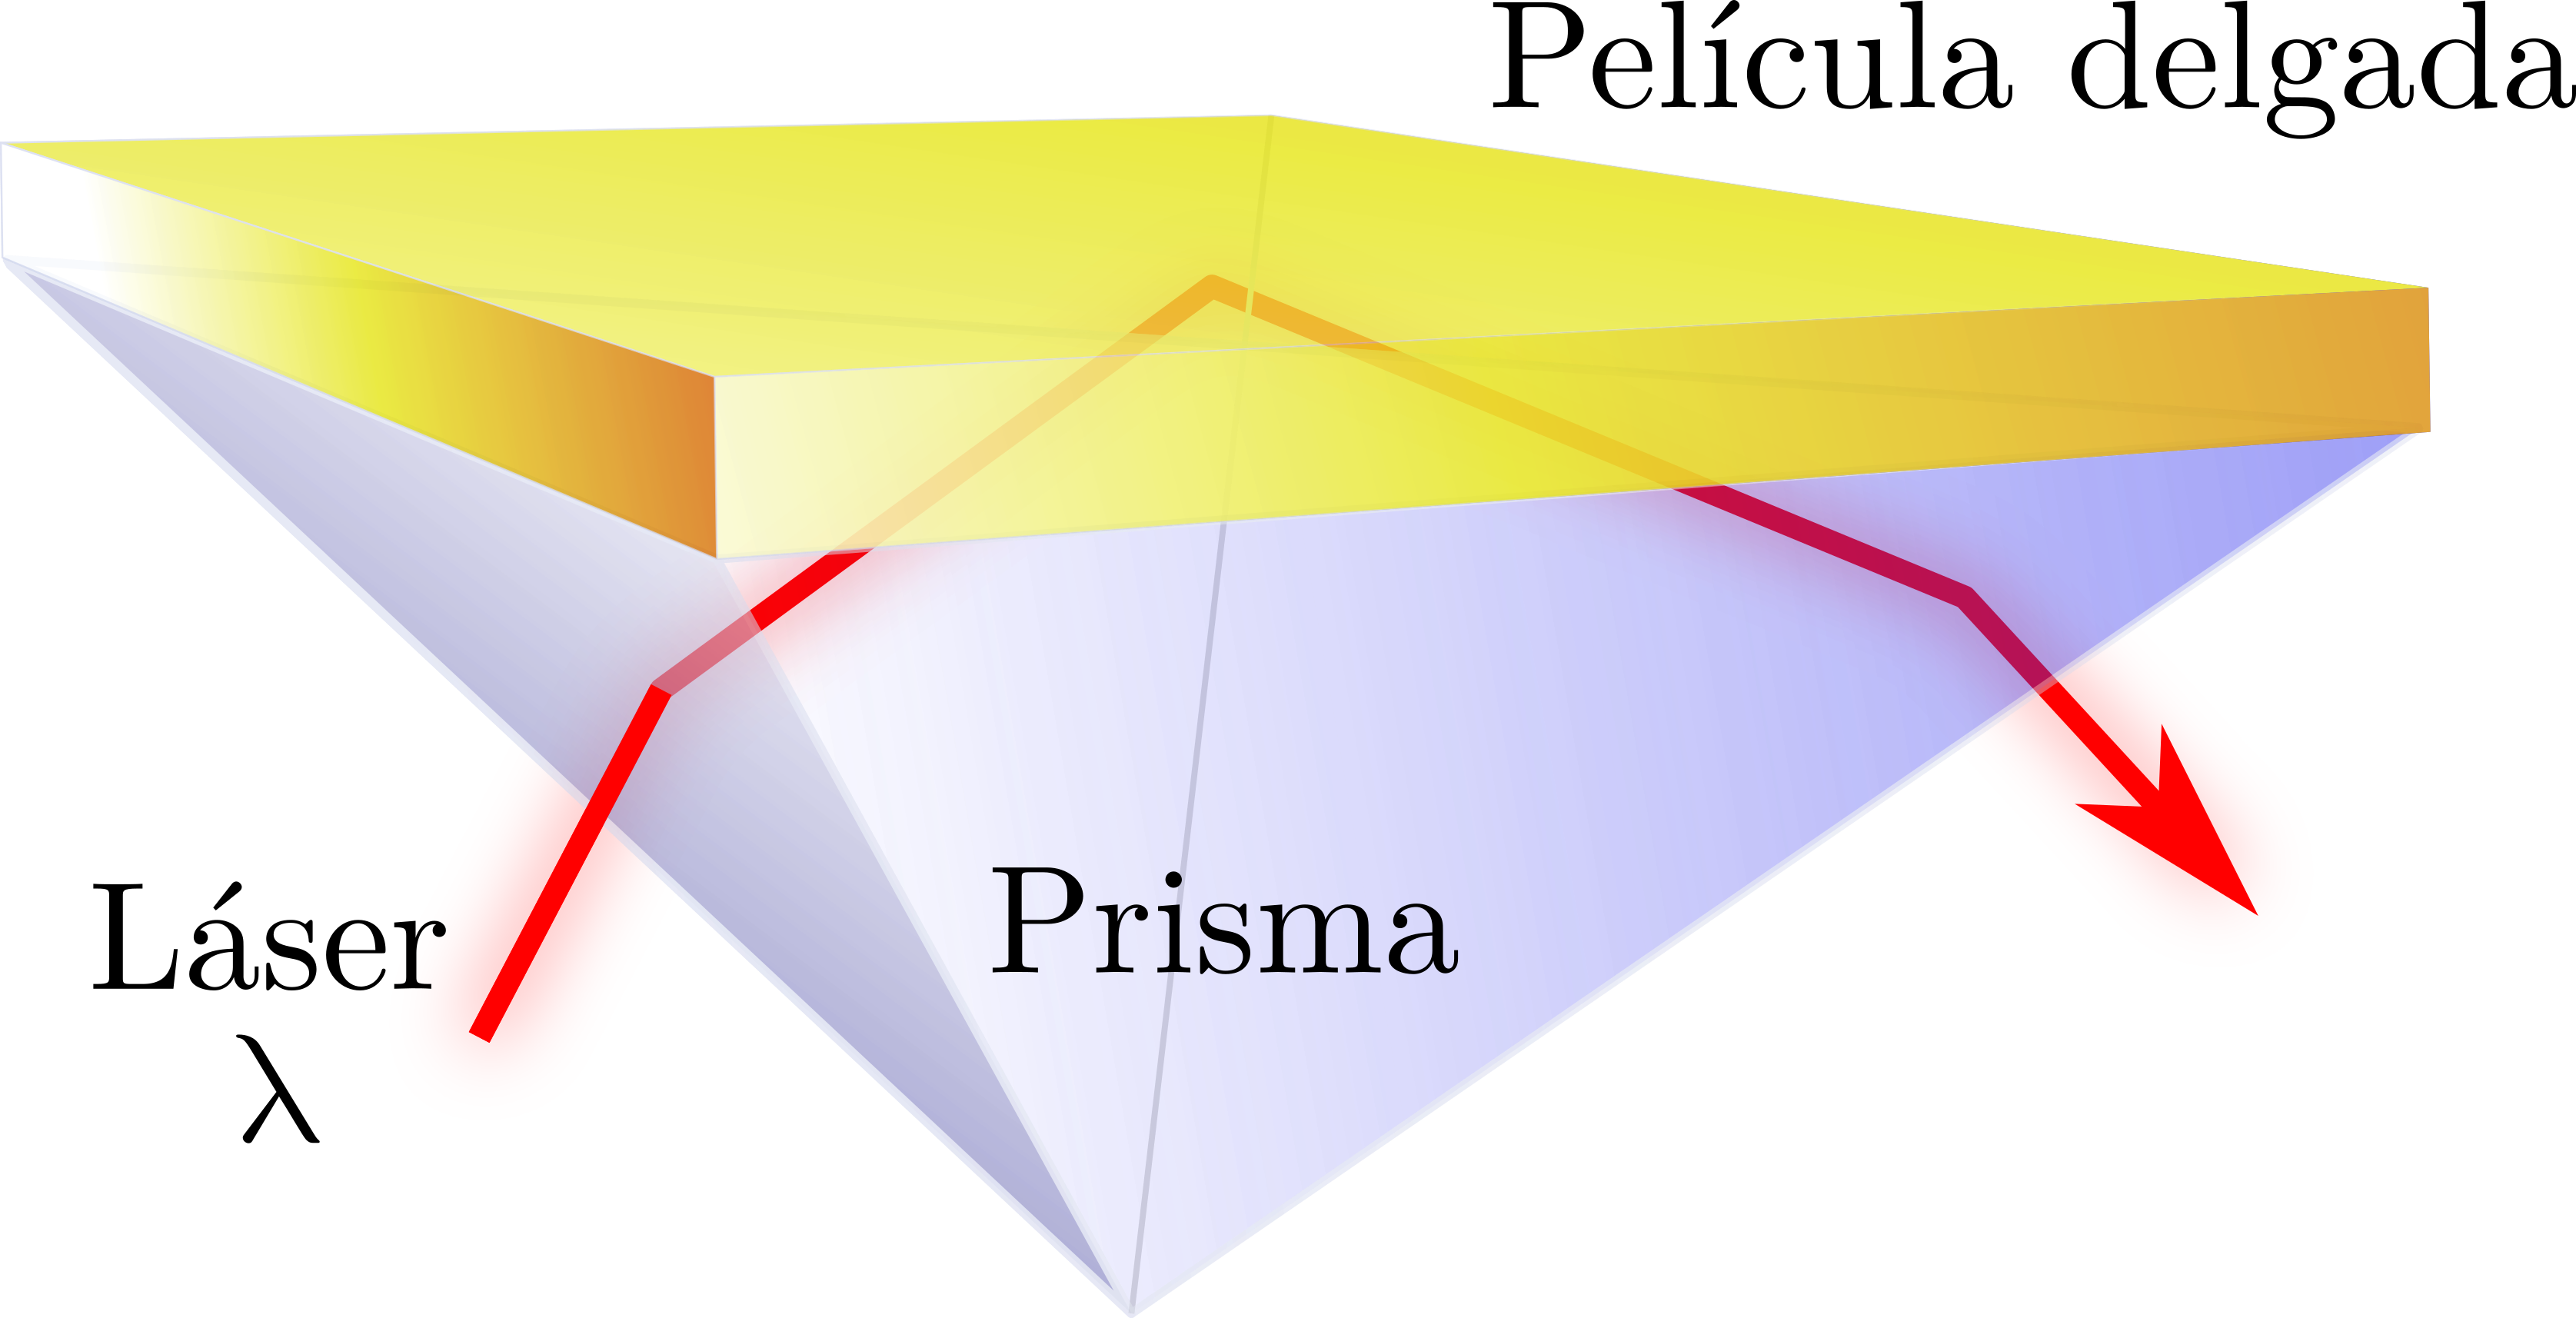
\includegraphics[scale=.225]{0-4-Introduccion/figs/SPP-3D.png}
		\end{subfigure}
	\begin{subfigure}{.05\textwidth}\vspace{-3.5cm}\caption{}\label{sfig:ATRNP}	\end{subfigure}
	\begin{subfigure}{.43\textwidth}  
		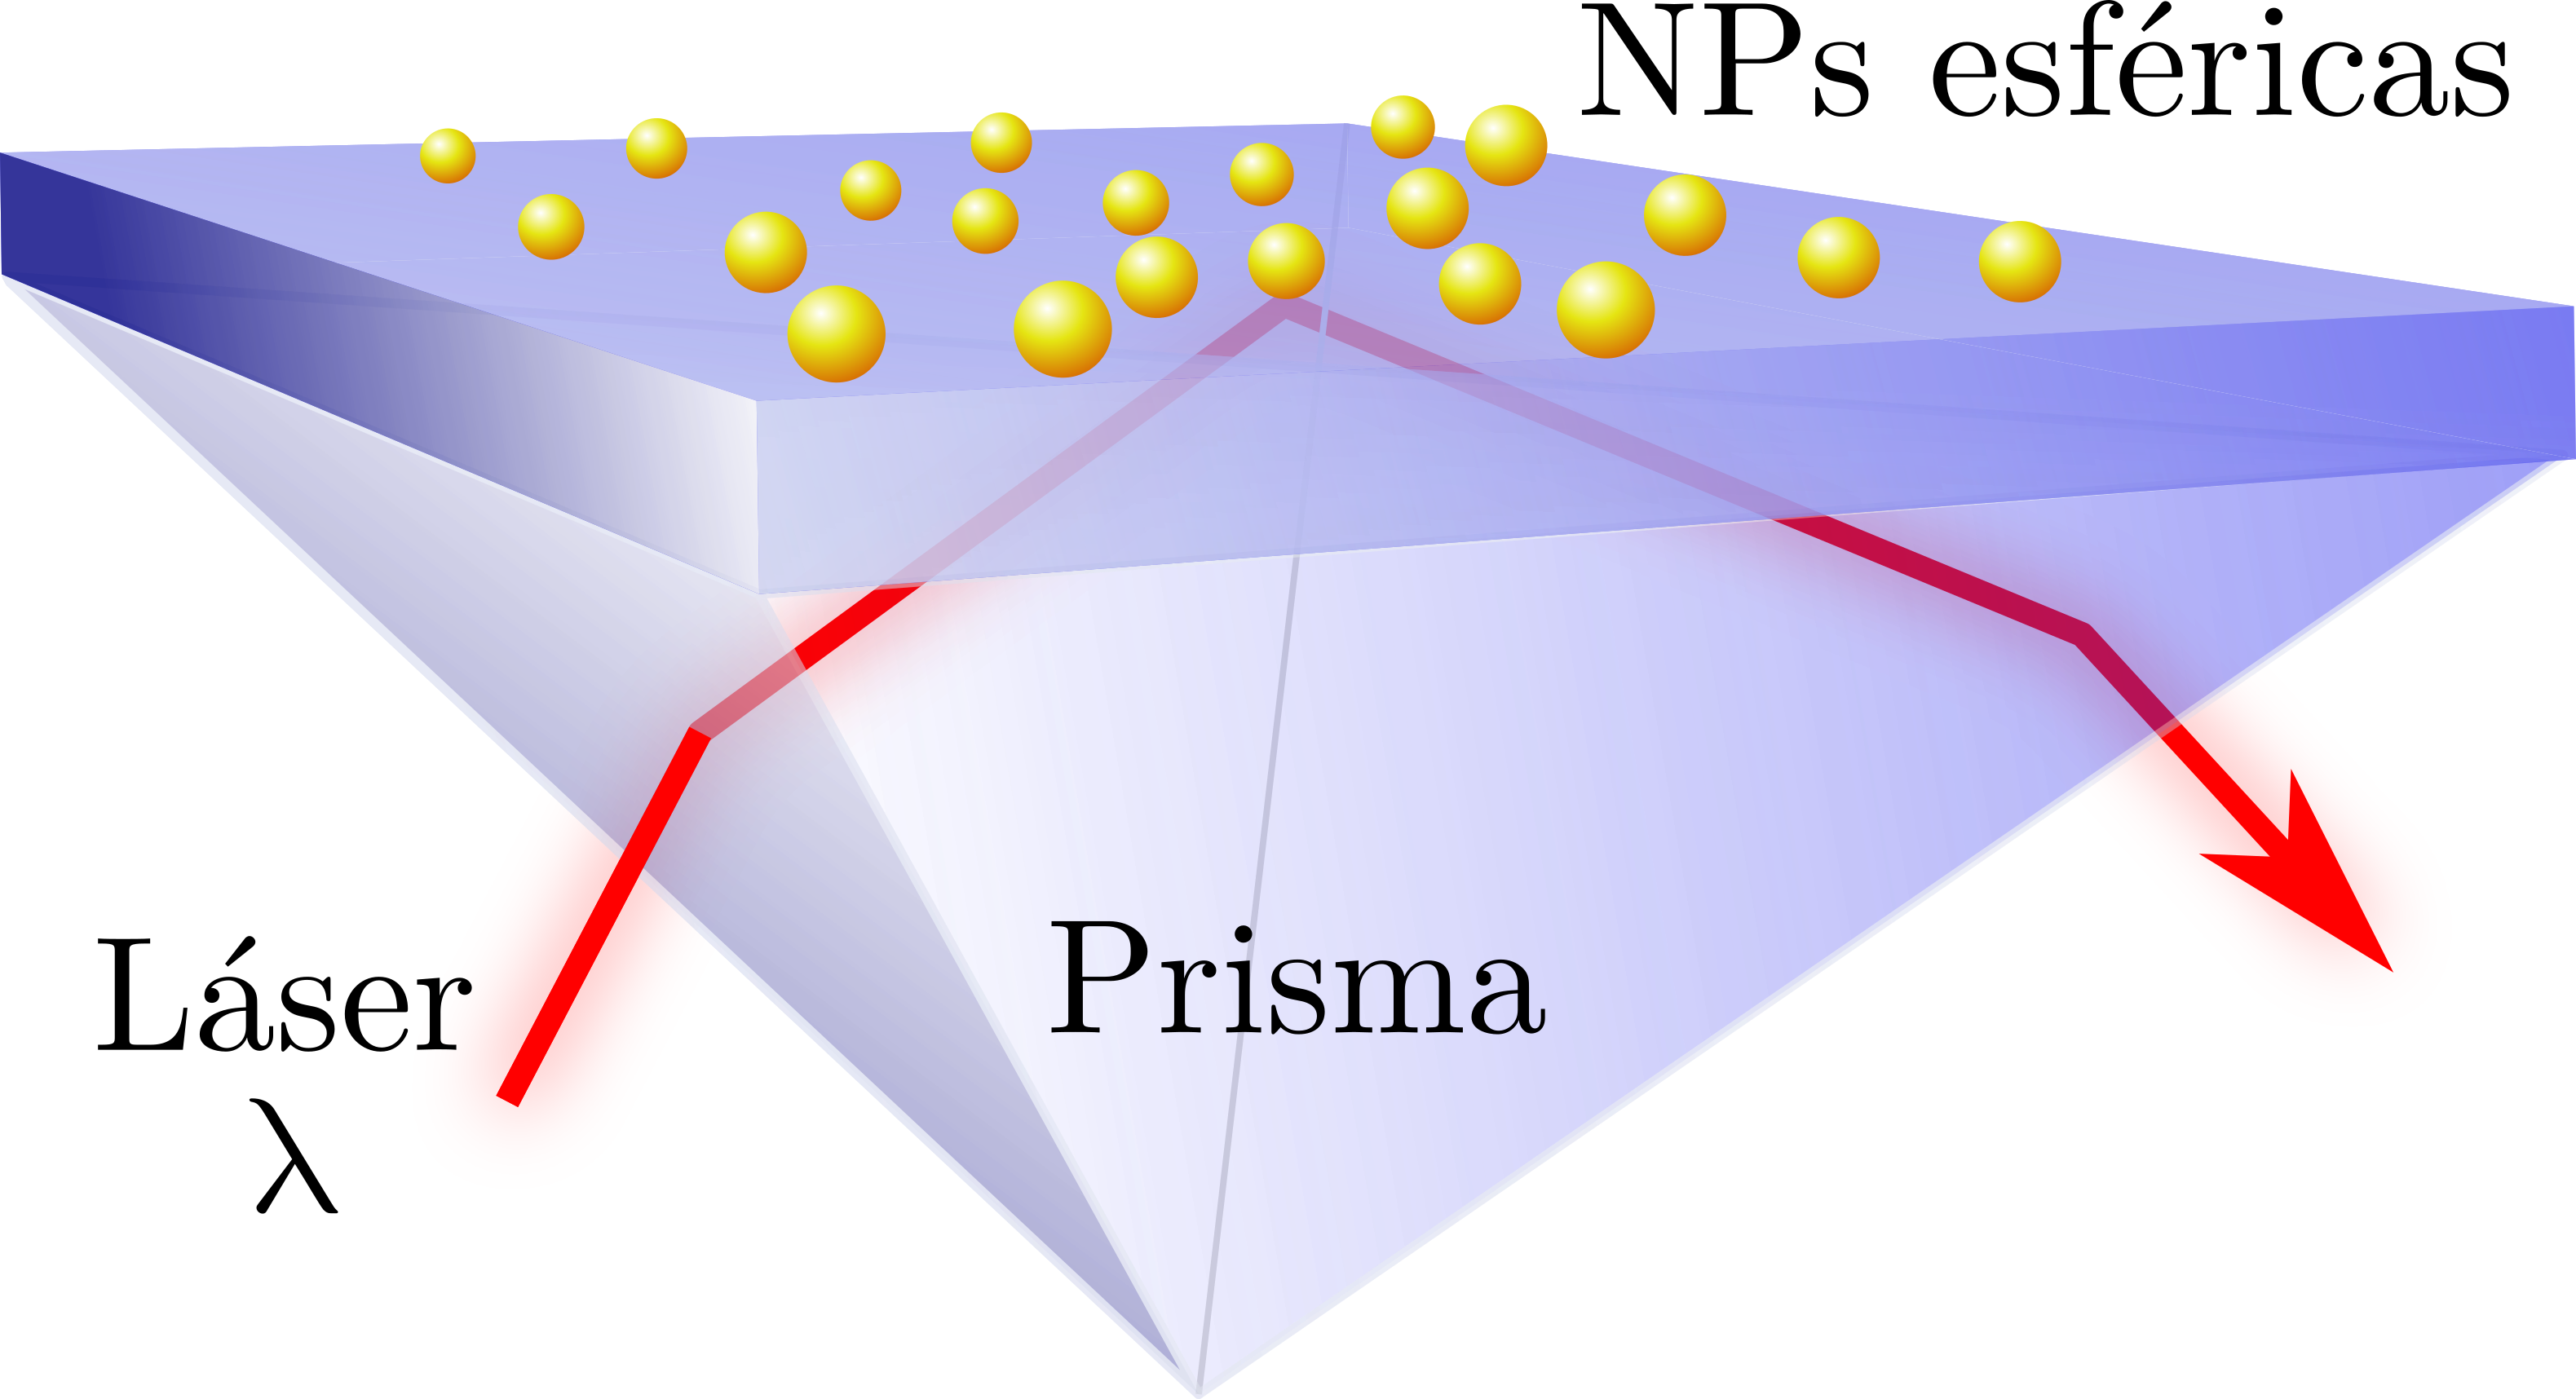
\includegraphics[scale=.225]{0-4-Introduccion/figs/NPs-3D.png}
	\end{subfigure} 
	\caption{ Iluminación de \textbf{a)} una película delgada y \textbf{b)} un arreglo de NPs esf\'ericas desordenadas por un haz óptico de longitud de onda $\lambda$, en configuraci\'on ATR.}	\label{fig:ATR1}	
	\end{figure}	
	
En el 2009 se public\'o un art\'iculo \cite{kabashin2009plasmonic} en el que se propone un sistema bidimensional de NPs cilíndricas de oro, localizadas periódicamente, para la mejora de la resoluci\'on  en el biosensado [ver Fig. \ref{sfig:Nanocilindros}]; las dimensiones de los nanocilindros y el parámetro de red del arreglo son menores que la longitud de onda con la que se ilumina el arreglo \cite{kabashin2009plasmonic}.  En el artículo se reportó un modo plasmónico distinto a los modos de las NPs individuales, que permite el sensado del índice de refracción de la matriz y se le denominó \textit{modo guiado} \cite{kabashin2009plasmonic}.  En el 2018 se publicó que este modo es una respuesta colectiva del arreglo periódico \cite{danilov2018ultra} y que depende del parámetro de red; en este artículo se le identificó como una \emph{resonancia de red de superficie plasmónica} (Plasmonic Surface Lattice Resonance, PSLR), las cuales ocurren cuando un rayo que se refracta por la estructura periódica excita una LSPR en los elementos de la estructura \cite{vakevainen2013plasmonic}; las PSLR dependen del  ángulo de incidencia y de la periodicidad del arreglo \cite{danilov2018ultra} y pueden acoplarse con la matriz o con el sustrato. En la Fig. \ref{sfig:DipATR} se reproducen las gráficas (extraídas de \cite{kabashin2009plasmonic}) de la reflectancia como función de la longitud de onda, para el arreglo mostrado en la Fig.  \ref{sfig:Nanocilindros}, en donde se consideró un sustrato de vidrio ($n=1.5$) y una matriz de aire ($n=1$), así como una monocapa de nanocilindros de $360$ nm de largo, $25$ nm de diámetro, con una separación entre ellos de $60$ nm. La respuesta EM del arreglo de nanocilindros   fue calculada al considerar a los cilindros como nanoesferoides y emplear una modificación del modelo de Maxwell Garnett \cite{atkinson2006anisotropic} ---que es una teoría de medio efectivo\footnote{Proceso de homogenización en donde se sustituye el medio heterogéneo por un medio continuo equivalente.  Este proceso se basa en la respuesta promedio del medio original cuando la longitud de onda de la luz incidente es grande en comparación a las dimensiones del sistema \cite{sihvola1999mixing}.}--- para la función dieléctrica efectiva de la monocapa $\varepsilon(\omega) = n^2 (\omega)$. En la Fig. \ref{sfig:k(w)Kobashin} se grafica la relación de dispersión  (energía como función de la  proyección perpendicular al sustrato del vector de onda) de la PSLR (puntos blancos), mientras que en la Fig.  \ref{sfig:dLambda} se grafican los resultados experimentales del corrimiento de la PSLR al cambiar el índice de refracción de la matriz (reproducida de \cite{danilov2018ultra}).

	\begin{figure}[h!]\centering
		\begin{subfigure}{.01\linewidth}\caption{ }\label{sfig:Nanocilindros} \vspace{5cm}	\end{subfigure}  
		\begin{subfigure}{.45\linewidth}\hspace*{-3em}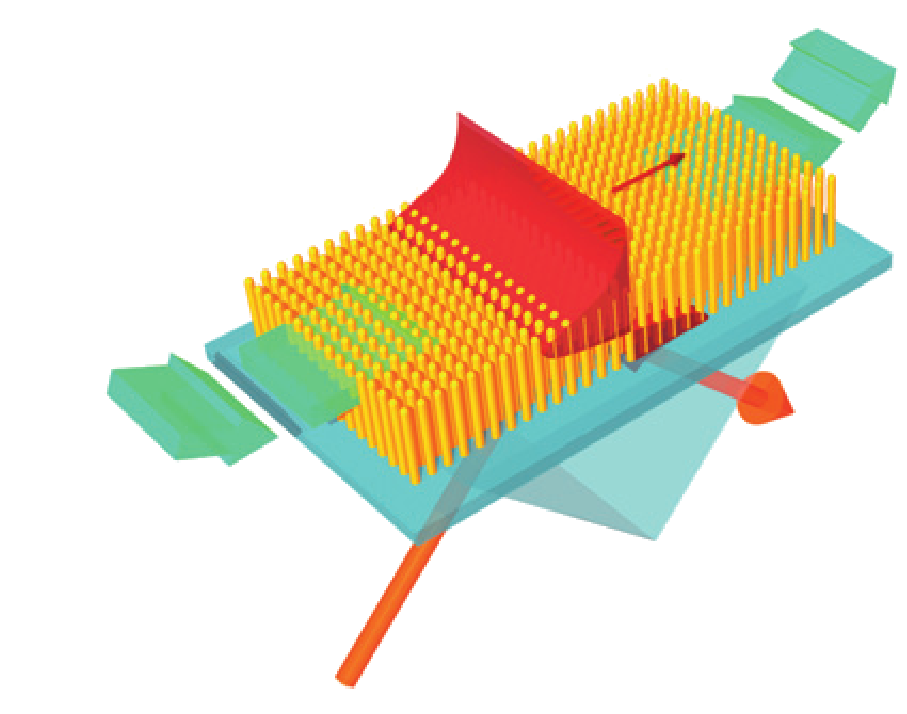
\includegraphics[scale=1]{0-4-Introduccion/figs/nanorods.png}\end{subfigure}
\begin{subfigure}{.01\linewidth}\caption{ }\label{sfig:DipATR}\vspace{4.75cm}\end{subfigure}  
		\begin{subfigure}{.45\linewidth}\hspace*{-1em}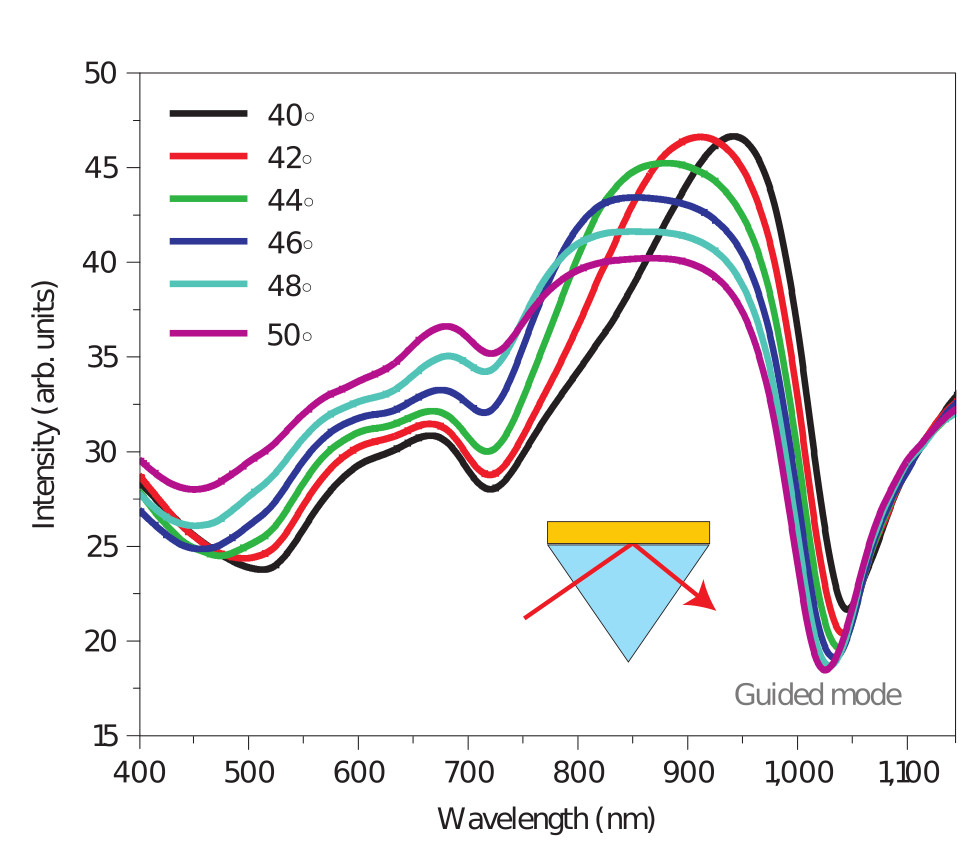
\includegraphics[scale=.9]{0-4-Introduccion/figs/reflectancia.png}\end{subfigure}\\
\begin{subfigure}{.01\linewidth}\caption{ }\label{sfig:k(w)Kobashin} \vspace{5cm}	\end{subfigure} 
		\begin{subfigure}{.45\linewidth}\hspace{1em}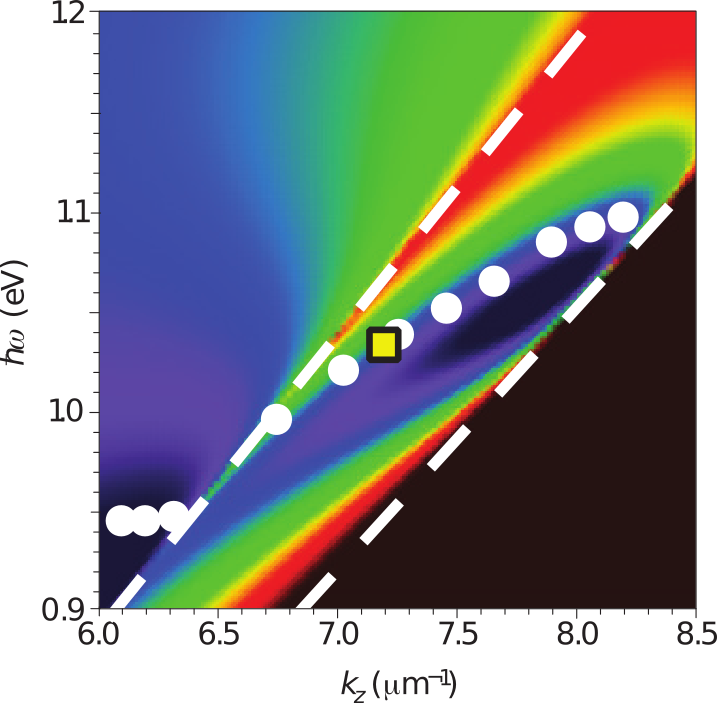
\includegraphics[scale=1]{0-4-Introduccion/figs/dispersion.png}\end{subfigure}	
\begin{subfigure}{.01\linewidth}\caption{ }\label{sfig:dLambda}\vspace{4.75cm}\end{subfigure}  
		\begin{subfigure}{.45\linewidth}\hspace*{-.5em}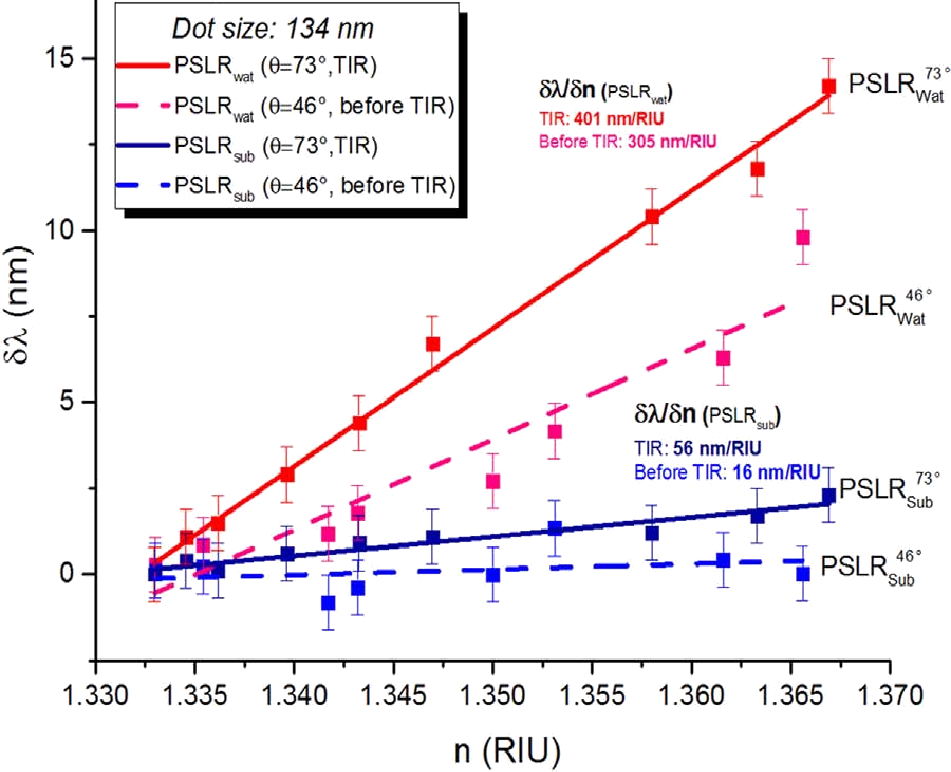
\includegraphics[scale=.9]{0-4-Introduccion/figs/sensibilidad.png}\end{subfigure}		
		\caption{\textbf{a)} Esquema de  un arreglo periódico cuadrado de nanocilindros de oro ---extraído de  \cite{kabashin2009plasmonic}---. \textbf{b)} Cálculos de la reflectancia ---extraídos de  \cite{kabashin2009plasmonic}--- como función de la longitud de onda $\lambda$, para distintos ángulos de incidencia, y \textbf{c)} de la relación de dispersión ---extraída de  \cite{kabashin2009plasmonic}---, considerando nanocilindros inmersos en una matriz de aire ($n=1$), sobre un sustrato de vidrio ($n=1.5$), de $360$ nm de largo, $25$ nm de diámetro y una separación de $60$ nm entre ellos. En \textbf{d)} se grafican los resultados experimentales ---extraídos de  \cite{danilov2018ultra}--- del corrimiento de las PSLR excitadas para un arreglo de nanocilindros inmersos en agua y soportados por un sustrato de vidrio para un ángulo de incidencia de $46^\circ$ y $73^\circ$; para este caso se emplearon cilindros de altura de $90$ nm, de diámetro de $134$ nm y una separación de $320$ nm. Las mediciones se realizaron cuando las oscilaciones del plasmón se acoplan con la matriz (PSLR$_{H_2{O}}$) y con el sustrato (PSLR$_{sus}$).}\label{fig:GraphsPapersNANOCILINDROS}
	\end{figure}

Los cálculos de la reflectancia en ATR [Fig. \ref{sfig:DipATR}], muestran las resonancias plasmónicas típicas de NPs individuales para cilindros (modo longitudinal alrededor de $720$ nm y el transversal alrededor de $500$ nm) y adicional a ellas, se observa la PSLR alrededor de los $1,050$ nm. La PSLR, al excitarse a energías menores del modo longitudinal, no puede corresponder a una resonancia de NP individual y por tanto debe corresponder a un modo colectivo. En la Fig.  \ref{sfig:k(w)Kobashin} se grafica la relación de dispersión de dicho modo, donde los puntos blancos corresponden a los mínimos en la reflectancia alrededor de $1,050$ nm de la Fig.  \ref{sfig:DipATR} de la PSLR.  Las líneas punteadas en la Fig.   \ref{sfig:k(w)Kobashin} corresponden a los ángulos críticos de las interfaces del medio efectivo simulado con el aire (línea superior izquierda) y con el sustrato (línea inferior derecha); la región oscura debajo de la línea punteada inferior derecha representa las combinaciones de energía y vector de onda sin sentido físico\footnote{La proyección del vector de onda perpendicular a la interfaz está dada por $k_z = (\omega / c)n_m\cos\theta_i$, donde $\omega$ y $\theta_i$ son la frecuencia angular y el ángulo de incidencia de la onda plana incidente, respectivamente. La combinación de $\hbar\omega$ y $k_z$ en la región negra de la Fig. \ref{sfig:k(w)Kobashin} corresponde a valores donde $\cos\theta_i>1$, dando como resultado un ángulo complejo de incidencia, por lo que no tiene sentido físico.}.  En la Fig.  \ref{sfig:dLambda} se muestra el corrimiento de la longitud de onda de excitación $\delta\lambda$ de las PSLRs como función del índice de refracción de la matriz $n$ ---medido en unidades de índice de refracción (Refractive Index Units, RIU)--- cuando un haz de luz que incide a $46^\circ$ (líneas punteadas) y  a $73^\circ$ (líneas sólidas) se difracta por la matriz de agua (líneas roja y magenta) y por el sustrato de vidrio (líneas azul y morado). Dentro de la gráfica se muestran los valores de la sensibilidad $\delta \lambda/\delta n$ para cada caso.  

%\section*{Planteamiento del problema}

Los biosensores basados es nanoestructuras periódicas ordenadas, como el de nanocilindros mostrado en la Fig. \ref{sfig:Nanocilindros}, pueden ser sintonizados a una longitud de onda particular al ajustar el parámetro de red del arreglo, permitiendo optimizar la medición del sensor para cada tipo de muestra, además de ser compatibles con equipos comerciales actuales \cite{kabashin2009plasmonic}.  Sin embargo, la fabricaci\'on de arreglos ordenados de NPs presenta una complicaci\'on t\'ecnica de alto costo y largo tiempo de fabricación \cite{estevez2014trends}, por lo que en esta tesis se propone el uso de un arreglo bidimensional desordenado de NPs esféricas que presente una respuesta colectiva semejante a la reportada en \cite{kabashin2009plasmonic} y \cite{danilov2018ultra}. Se ha observado que la respuesta colectiva en un arreglo desordenado también es sintonizable según las propiedades de las NPs empleadas, por lo que su uso en sensado no sólo cuenta con las ventajas de los sensores propuestos en \cite{kabashin2009plasmonic} y \cite{danilov2018ultra}, sino también una reducción en los precios y tiempos de fabricación. 

%\section*{Metodología}
Para  caracterizar la respuesta óptica de un arreglo bidimensional desordenado de NPs esféricas plasmónicas se emplea el modelo de esparcimiento coherente (Coherent Scattering Model, CSM) \cite{reyes2018analytical}, el cual proporciona expresiones analíticas para los coeficientes de amplitud de reflexión y de transmisión para una monocapa de NPs esféricas, idénticas, y desordenadas.  Las expresiones  dadas por el CSM dependen de las componentes de la matriz de esparcimiento que aparece en la solución de Mie ---que resuelve los campos EMs esparcidos por una esfera iluminada por una onda plana monocromática \cite{bohren1998absorption}---, así como la respuesta EM del material con que están hechas las partículas esféricas de la monocapa: la función dieléctrica $\varepsilon(\omega)$.  Para caracterizar una excitación equivalente a la PSLR estudiada en \cite{kabashin2009plasmonic} y \cite{danilov2018ultra}, es decir, una respuesta colectiva apta para el biosensado, se calcula la reflectancia y transmitancia del sistema monocapa mediante los coeficientes de amplitud de reflexión y transmisión del CSM. 
 
Adicional a la caracterización de la respuesta óptica de una monocapa desordenada de NPs esféricas e idénticas dada por el CSM, se realiza una comparación entre ésta y la respuesta óptica de los biosensores comerciales basados en SPPs. La comparación se realiza mediante un análisis de sensibilidad (el corrimiento de la longitud de onda de la resonancia respecto al cambio del índice de refracción de la matriz $\delta\lambda_{res}/\delta n$) y de la \emph{figura de mérito} (Figure Of Merit, FoM) de bulto $\textit{FoM}_B$ ---definida como $(\delta\lambda_{res}/\delta n)/\Gamma$, con $\Gamma$ la anchura a media altura (Full Width at Half Maximum, FWHM)---, como se  efectúa en \cite{svedendahl2009refractometric}, donde se compara experimentalmente la respuesta óptica de una monocapa desordenada de nanodiscos (NDs)  de oro [ver Fig. \ref{sfig:NanoDisks}] con la de una película continua de oro. Los NDs empleados en \cite{svedendahl2009refractometric} son nanocilindros de $30$ nm de altura y  $120$ nm de diámetro\footnote{En \cite{svedendahl2009refractometric} no se da información sobre la fracción de cubierta ni de la distancia mínima promedio entre NDs.}, mientras que el grosor de la película continua es de $50$ nm: estos parámetros sintonizan la LSPR de los ND y el SPP a $700$ nm, considerando $\theta_i=70^\circ$. En la Fig. \ref{sfig:TNanoD} se grafica la longitud de onda de resonancia  $\lambda_{res}$ del arreglo desordenado de NDs, que coincide con la LSPR de los nanocilindros individuales, como función del ángulo de incidencia $\theta_i$; los valores de $\lambda_{res}$ corresponden a los mínimos de la transmitancia graficada en el recuadro dentro de la Fig. \ref{sfig:TNanoD}. En la Fig. \ref{sfig:resumenNDs} \textbf{i)} se grafican la reflectancia y la transmitancia  en una configuración de iluminación directa del arreglo desordenado de NDs, mientras que en la Fig. \ref{sfig:resumenNDs} \textbf{ii)} se grafica la reflectancia, en configuración ATR, para la película continua de oro, en ambos caso se considera una matriz de agua ($n=1.33$) y de agua con distintas concentraciones de etilenglicol. Finalmente, en la Fig. \ref{sfig:resumenNDs} \textbf{iii)} se grafica el corrimiento de la resonancia $\delta\lambda_{res}$ como función del índice de refracción de la matriz; la sensibilidad tanto del SPP como la LSPR de los NDs se muestran dentro de la gráfica. A partir de la Fig. \ref{sfig:resumenNDs} se concluye en \cite{svedendahl2009refractometric} que la sensibilidad del SPP ($3,300$ nm~\mbox{RIU$^{-1}$}) es mayor a la del arreglo desordenado de NDs ($178$ nm~\mbox{RIU$^{-1}$}), lo cual también ocurre con las FoM: para el SPP se obtiene que $\textit{FoM}_{B,\textit{SPP}}\approx 57 \mbox{ RIU$^{-1}$}$, mientras que para los ND $\textit{FoM}_{B,\textit{ND}}\approx 2\mbox{ RIU$^{-1}$}$. Los resultados reportados en \cite{svedendahl2009refractometric} para la sensibilidad y la $\textit{FoM}_B$ son consistentes con lo reportado en la literatura \cite{brian2009sensitivity,cahill1997surface}.
 
\begin{figure}[t!]\centering
\begin{minipage}[c]{.48\linewidth}
		\begin{subfigure}{.01\linewidth}\caption{ }\label{sfig:NanoDisks} \vspace{4.cm}	\end{subfigure}  
		\begin{subfigure}{.98\linewidth}\hspace*{3em}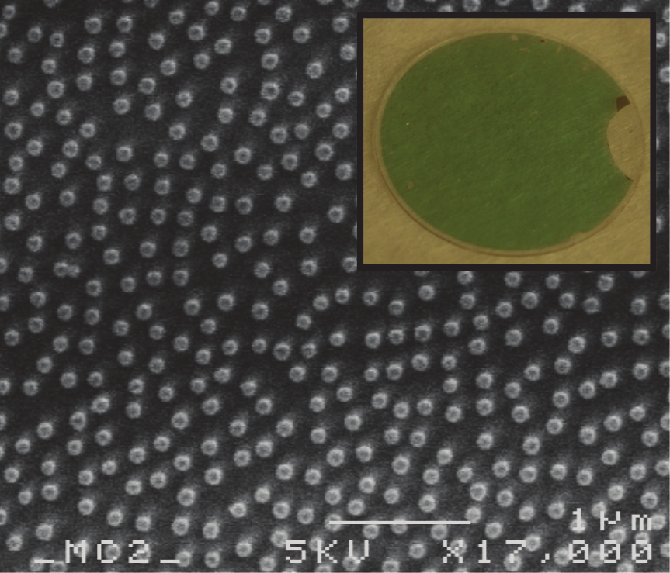
\includegraphics[scale=1.]{0-4-Introduccion/figs/nanoDisk.png}\end{subfigure}\\
\noindent \begin{subfigure}{.01\linewidth}\caption{ }\label{sfig:TNanoD}\vspace{3.5cm}\end{subfigure}  
		\begin{subfigure}{.98\linewidth}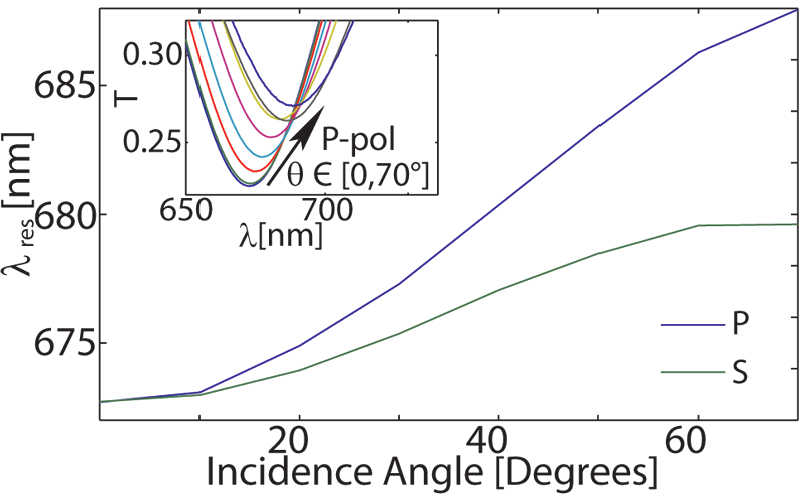
\includegraphics[scale=1.1,trim={0 0 0 -1em},clip]{0-4-Introduccion/figs/TransmitanciaND.png}\end{subfigure}
\end{minipage}		
		\begin{subfigure}{.01\linewidth}\caption{ }\label{sfig:resumenNDs} \vspace{9cm}	\end{subfigure} 
		\begin{subfigure}{.48\linewidth}\hspace{.5em}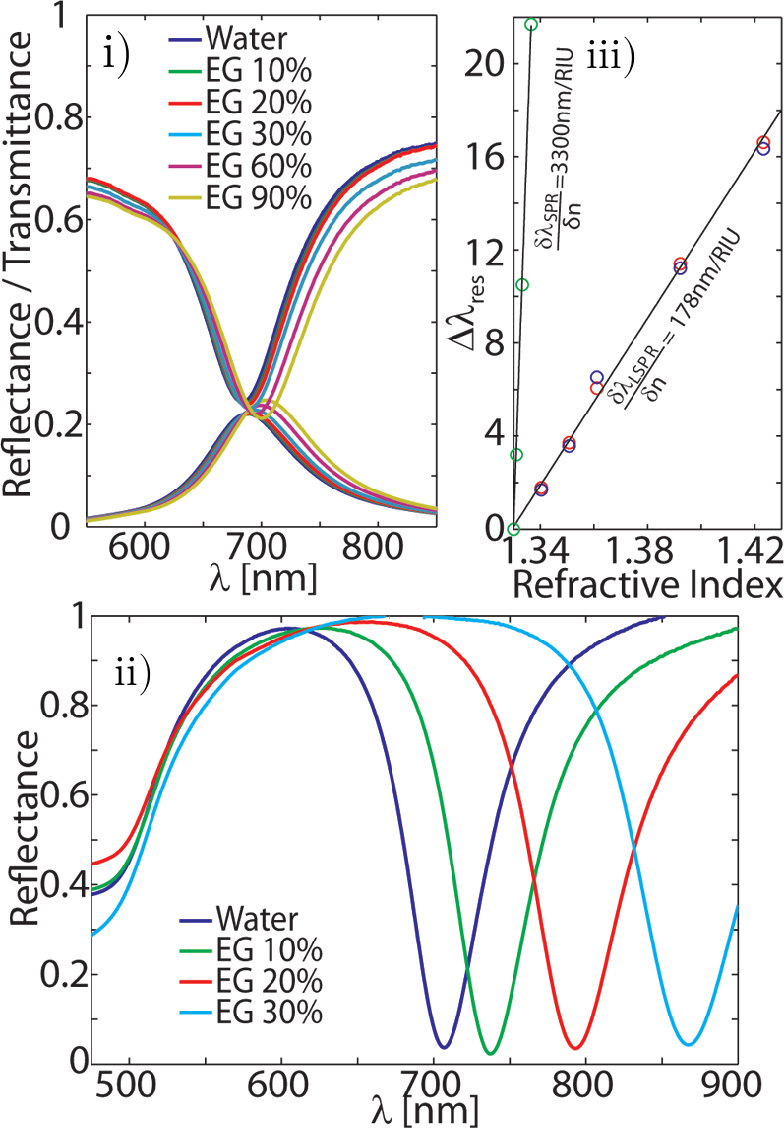
\includegraphics[scale=1.05]{0-4-Introduccion/figs/resumenND.png}\end{subfigure}		
		\caption{ \textbf{a)} Micrografía de electrones de barrido de la muestra del arreglo desordenado de NDs ---nanocilindros de $30$ nm de altura y  $120$ nm de diámetro--- de oro sobre vidrio. El recuadro interior muestra una fotografía de la muestra con un sustrato de $2.5$ cm de diámetro. \textbf{b)} Gráfica de la longitud de onda de resonancia $\lambda_{res}$ del arreglo desordenado de NDs como función del ángulo de incidencia para ambas polarizaciones: \emph{s} y \emph{p}. Los valores de $\lambda_{res}$ corresponden a los mínimos de la transmitancia graficada dentro del recuadro. \textbf{c)} Gráfica \textbf{i)} de la transmitancia y reflectancia del arreglo de NDs en iluminación directa y \textbf{ii)} de la reflectancia de una película delgada de oro de $50$ nm de grosor en una configuración ATR como función de la longitud de onda $\lambda$, considerando una matriz de agua ($n=1.33$) y de agua con distintas concentraciones  de etilenglicol; \textbf{iii)} corrimiento de $\lambda_{res}$ presente en la película delgada y en el arreglo de NDs; el valor de la sensibilidad de cada arreglo se encuentra dentro de la gráfica. Todas las gráficas fueron extraídas de \cite{svedendahl2009refractometric}.}\label{fig:GraphsPapersNANODISKS}
	\end{figure} 
 
El objetivo de esta tesis de licenciatura es caracterizar la respuesta EM de una monocapa desordenada de NPs esféricas idénticas soportada por un sustrato, calculando la reflectacia y transmitancia de forma analítica por el formalismo del CSM (considerando monocapas formadas por NPs de oro y de plata), y compararla tanto con la de una película continua de $50$ nm de grosor (sistema empleado en biosensores comerciales) \cite{svedendahl2009refractometric}, como con la de una monocapa de nanocilindros ordenados \cite{kabashin2009plasmonic,danilov2018ultra} y con la de una monocapa de nanodiscos desordenados \cite{svedendahl2009refractometric}, y evaluar si el sistema de NPs esféricas desordenadas es apto para el biosensado.

Para determinar si una monocapa desordenada de nanopartículas esféricas puede ser empleada como biosensor, se realizaron cálculos de la reflectancia en ATR para una monocapa de NPs embebidas en agua y soportadas por un sustrato de vidrio, considerando que la función dieléctrica de las NPs en la monocapa está dada por el modelo de Drude-Sommerfeld. Se caracterizó un modo plasmónico distinto a las SPRs de partículas individuales mediante variaciones del radio de las NPs y de la fracción de cubierta de las monocapa. Es decir, primero se estudió el supuesto modo plasmónico colectivo para una monocapa de NPs ideales, y posteriormente se estudiaron monocapas con NPs de materiales reales: oro y plata. Mediante la caracterización, variando nuevamente el radio de las NPs de la monocapa y la fracción de cubierta de ésta, se determinaron los parámetros óptimos para que las monocapas de NPs de oro y de plata sean propuestas como biosensores. Finalmente, se comparó la sensibilidad del supuesto modo plasmónico colectivo ante cambios en el índice de refracción de la matriz donde están embebidas las NPs con la sensibilidad del SPP excitado en una película continua de oro de $50$ nm (sensores comerciales) y con propuestas de arreglos nanoestructurados para el biosensado publicados en \cite{kabashin2009plasmonic,danilov2018ultra,svedendahl2009refractometric}; asimismo se calcularon las FoM de bulto para el supuesto modo plasmónico colectivo y para el SPP considerado tanto oro como plata para las NPs en la monocapa y para la película continua.

Esta tesis está dividida en tres partes: Teoría (capítulo \ref{chapter:Teoria}), Respuesta óptica de una monocapa desordenada de nanopartículas esféricas (capítulo \ref{chapter:Resultados}) y Conclusiones. En el capítulo \ref{chapter:Teoria}, se presentan en la sección \ref{section:NocionesBasicas} la solución tipo ondas planas de las ecuaciones de Maxwell y las ecuaciones de Fresnel para describir el comportamiento de una onda plana monocromática al incidir sobre una superficie plana entre dos medio materiales lineales, homogéneos e isótropos, mientras que en la sección \ref{section:Mie} se estudia la solución de Mie, que resuelve las ecuaciones de Maxwell para una partícula esférica, empleando la matriz de esparcimiento que relaciona los campos EMs esparcidos por la esfera con los campos EMs incidentes, explicando el problema de absorción y esparcimiento de luz por una partícula esférica de material y tamaño arbitrario. En la sección \ref{section:RespuestaEM} se estudia la respuesta EM de materiales plasmónicos en bulto y a escala nanométrica: en la subsección \ref{ssection:Drude} se presenta el modelo de Drude-Sommerfeld (respuesta EM de un gas de electrones libres) para la función dieléctrica, mientras que en la sección \ref{ssection:CorreccionTamano} se presenta un método para determinar los parámetros del modelo de Drude-Sommerfeld que ajustan a los datos experimentales de la función dieléctrica del oro y de la plata, así como una corrección por tamaño de la función dieléctrica para NPs esféricas; asimismo, en la sección \ref{ssection:Plasmones} se presentan los plasmones, que son oscilaciones colectivas resultado del acoplamiento entre una onda plana y los electrones libres de algún material. En la  sección \ref{section:CSM} se estudia el CSM, que proporciona expresiones analíticas para los  coeficientes de amplitud de reflexión y de transmisión de una monocapa desordenada de NPs esféricas e idénticas, suspendida en el espacio libre (sección \ref{ssection:FSM}) y  soportada por un sustrato (sección \ref{ssection:CSMATR}), cuando una onda plana monocromática incide sobre la monocapa. Posteriormente, en el capítulo \ref{chapter:Resultados}, se presentan en la sección \ref{section:Drude} los resultados de la reflectancia de una monocapa de NPs con una función dieléctrica tipo Drude, suspendida en el espacio libre (subsección \ref{ssection:DrudeFSM}) y soportada por un sustrato e iluminada en una configuración ATR (subsección \ref{ssection:DrudeATR}). En la sección \ref{section:AuAg} se presentan los resultados de la reflectancia en una configuración ATR de un monocapa de NPs de oro y de plata y en la sección \ref{section:sensLambda} se realiza un análisis de sensibilidad para una monocapa de NPs esféricas de oro y se compara con la de una película continua de oro $50$ nm de grosor y con la propuestas de sistemas nanoestructurados. Por último, se escriben las conclusiones, con base en los resultados del capítulo \ref{chapter:Resultados}, para el posible empleo de una monocapa de NPs de oro y de plata como biosensor, así como trabajo a futuro.
            
\chapter{Teoría}

 En este capítulo se estudia la interacción de la luz con la materia, caracterizada por una función dieléctrica dependiente de la frecuencia, que se modifica según el tamaño y la geometría del objeto. En la primera sección se presentan la  solución de ondas planas a las ecuaciones de Maxwell y las condiciones que se imponen a los campos electromagnéticos (EMs) al propagarse a través de un medio homogéneo, lineal e isótropo, y al cruzar una interfaz arbitraria a otro medio con las mismas características, así como el caso particular de la reflexión y transmisión de una onda plana al cruzar una interfaz plana, que deviene en las fórmulas de Fresnel. En la segunda sección se presenta la solución de Mie, que consiste en la solución al problema de absorción y esparcimiento de luz debido a una partícula esférica de tamaño y material arbitrario al ser iluminada por una onda plana y monocromática, dando como resultado los campos EMs esparcidos por la partícula. En la tercera sección se presenta el modelo de Drude-Sommerfeld como respuesta EMs de materiales plasmónicos mediante la función dieléctrica, así como un método para ajustar las mediciones experimentales de la función dieléctrica y poder hacer la corrección de tamaño para partículas esféricas \emph{pequeñas}; asimismo se definen los plasmones ---acoplamiento de la luz con los electrones libres de un material--- al considerar materiales cuya respuesta EM es descrita por el modelo de Drude-Sommerfeld, así como el caso para materiales más realistas. Finalmente, en la cuarta sección, se presenta la respuesta EM de una monocapa de partículas esféricas idénticas, descrita por el modelo de esparcimiento coherente (Coherent Scattering Model, CSM) en donde se calculan los coeficientes de amplitud de reflexión y transmisión para un sistema que considere una monocapa de NPs esféricas idénticas, inmersa en un medio dieléctrico (denominado matriz) y soportada por un sustrato dieléctrico.

\section{Ecuaciones de Maxwell y fórmulas de Fresnel}

Las ecuaciones de Maxwell en su forma diferencial están dadas por las expresiones   \cite{griffiths2013electrodynamics}  \index{Maxwell!ecuaciones de} \vspace*{-.75em}
%
	\begin{subequations} \label{eqs:Maxwell}
	\begin{tcolorbox}[title = Ecuaciones de Maxwell en el sistema internacional de unidades,
	ams align, breakable]
	\nabla \cdot\vb{E} &= \frac{\rho_{tot}}{\varepsilon_0}, &\mbox{(Ley de Gauss eléctrica)}  
	\label{seq:GE} \\
	\nabla \cdot\vb{B} &= 0,						&\mbox{(Ley de Gauss magnética)}   
	\label{seq:GM} \\
	\nabla \times\vb{E} &= -\pdv{\vb{B}}{t}, 	&\mbox{(Ley de Faraday-Lenz)}		
	\label{seq:FL}\\
	\nabla \times\vb{B} &= \mu_0 \vb{J}_{tot} +\varepsilon_0\mu_0 \pdv{\vb{E}}{t}, &
	\mbox{(Ley de Ampère-Maxwell)} \label{seq:AM}
	\end{tcolorbox}\end{subequations}\vspace*{-.75em}\noindent
%
donde $\vb{E}$ es el campo eléctrico y $\vb{B}$, el campo magnético; $\rho_{tot}$ es la densidad volumétrica de carga total  y $\vb{J}_{tot}$, la densidad volumétrica de corriente total; $\varepsilon_0$ es la permitividad eléctrica del vacío y $\mu_0$, la permeabilidad magnética del vacío.

Al desacoplar las ecuaciones de Maxwell, los campos EMs obedecen la ecuación de onda \cite{hecht1998optics}, \index{Ecuación!de onda} que al emplear la transformada Fourier\footnote{\setstretch{1.0} $\mathcal{F}[f(\vb{r},\omega)] = \int_{-\infty}^\infty f(\vb{r},t) e^{i(\vb{k}\cdot\vb{r} -\omega t)} dt$, con $\vb{k}$ una función de $\omega$. La transformada de Fourier inversa es entonces $\mathcal{F}^{-1}[f(\vb{r},t)] =\frac{1}{2\pi} \int_{-\infty}^\infty f(\vb{r},\omega) e^{i(\vb{k}\cdot\vb{r} -\omega t)} d\omega$.\index{Fourier!transformada de}} y considerar una región del espacio sin fuentes ($\rho_{tot}=0$ y $\vb{J}_{tot}=\vb{0}$), se obtiene la ecuación de Helmholtz \index{Ecuación!de Helmholtz} para $\vb{E}$ y $\vb{B}$ \cite{griffiths2013electrodynamics}

	\begin{subequations}\eqhalf{\nabla^2\vb{E} + k^2 \vb{E}=\vb{0},}
	\eqhalf{\nabla^2\vb{B} + k^2 \vb{B}=\vb{0}.}\end{subequations}\vspace*{-1em}

\noindent Una de las soluciones a la ecuación de Helmholtz para los campos EMs son las ondas planas, es decir, que los campos EMs son de la forma \cite{jackson1999electrodynamics} \index{Maxwell!ecuaciones de!solución de ondas 
planas a las}\index{Onda!plana}\index{Onda!plana!en la base cartesiana canónica}

	\begin{subequations}\eqhalf{\vb{E}(\vb{r},t) =\vb{E_0}e^{i(\vb{k}\cdot\vb{r} -\omega t)},}
	\eqhalf{\vb{B}(\vb{r}, t) =\vb{B_0}e^{i(\vb{k}\cdot\vb{r} -\omega t),}}	
	\label{eqs:ondasPlanas}\end{subequations}\vspace*{-1em}
		
\noindent en donde  $\vb{E_0}$ y $\vb{B_0}$ representan las amplitudes de los campos EMs, $\vb{k}$ es el vector de onda y $\omega$ es la frecuencia angular; la triada de vectores \{$\vb{k},\, \vb{E},\, \vb{B}$\} constituye una base ortogonal derecha en el vacío \cite{griffiths2013electrodynamics}. Para un medio material caracterizado por una función dieléctrica $\varepsilon(\omega)$ y una permeabilidad magnética $\mu$, se define el índice de refracción del medio $n(\omega)$ como \index{Índice de refracción}\index{Índice de refracción|seealso{Función dieléctrica}}\index{Función dieléctrica}\vspace*{-.75em}
%
	\begin{tcolorbox}[title = Índice de refracción, ams align]
	n(\omega) = \sqrt{\frac{\mu\varepsilon(\omega)}{\varepsilon_0 \mu_0}}.
		\label{eq:indice} 
	\end{tcolorbox}\vspace*{-.75em}\noindent
%
Tanto $n(\omega)$, como $\varepsilon(\omega)$ y $\mu$ se determinan de forma experimental y son, en general, cantidades complejas. Para que las ondas planas sean solución de las ecuaciones de Maxwell, se impone la relación de dispersión, que relaciona a  la magnitud del vector de onda $k$ con la frecuencia angular $\omega$ a obedecer la expresión \vspace*{-.75em}\index{Relación de dispersión}\index{Relación de dispersión!de una onda plana}
%
	\begin{tcolorbox}[title = Relación de dispersión, ams align]
	k(\omega) = \frac{\omega}{c}n(\omega)
	\label{eq:dispersion}
	\end{tcolorbox}\vspace*{-.75em}\noindent
%
en donde  $c=\sqrt{1/\varepsilon_0\mu_0}$ es la velocidad de la luz.

A partir de las ecuaciones de Maxwell se construye el teorema de conservación de la energía \cite{griffiths2013electrodynamics}, escrito en términos del vector de Poynting $\vb{S}$\index{Poynting!vector de}, que representa el flujo de energía EM por unidad de tiempo y unidad de área. Al considerar campos EMs de la forma de ondas planas [Ec. \eqref{eqs:ondasPlanas}], el vector de Poynting está dado por \cite{hecht1998optics}\vspace*{-.75em}
%
	\begin{tcolorbox}[title = Vector de Poynting, ams align]
	\vb{S} = \vb{E}\times\vb{H}^*,  \label{eq:Poynting}
	\end{tcolorbox} \vspace*{-.75em}\noindent
%
en donde $\vb{H}=\vb{B}/\mu$ es el campo H y $*$ corresponde a la operación complejo conjugado.

Las ecuaciones de Maxwell imponen condiciones a la frontera sobre los campos EMs cuando estos cruzan la frontera entre dos medios distintos, denominada interfaz. En la Fig. \ref{fig:GaussAmpere} se muestra la interfaz entre dos medios arbitrarios caracterizados por la función dieléctrica $\varepsilon_i$ y la permeabilidad magnética $\mu_i$, con $i = 1,\,2$ dependiendo del medio. Para deducir las condiciones a la frontera de los campos EMs sobre la interfaz, con vector normal $\vu{u}$, se evalúan los campos EMs en un cilindro con caras de área $A$ y altura $\delta$ [ver Fig. \ref{sfig:GaussPillbox}], así como  en un circuito de largo $l$ y altura $\delta$ [ver Fig. \ref{sfig:AmperianLoop}]. Al considerar el límite $\delta \to 0$, evaluando los campos EMs sobre la interfaz, la ausencia de fuentas externas ($\sigma_{ext} = 0$ y $\vb{K}_{ext} = \vb{0}$) y que los medios que conforman a la interfaz son lineales, homogéneos e isótropos, los campos EMs obedecen las  expresiones \cite{griffiths2013electrodynamics}:\vspace*{-.75em}\index{Electromagnéticos!campos!condiciones a la frontera de los}
%
	\begin{subequations}
	\begin{tcolorbox}[title = Condiciones de frontera de los campos EMs sin fuentes externas]
	\eqhalf{\varepsilon_1 E^\perp_1 - \varepsilon_2 E^\perp_2 = 0, \label{seq:Eperp}}
	\eqhalf{\vb{E}_1^\parallel -\vb{E}_2^\parallel = \vb{0},\label{seq:Epara}}\vspace*{.5em}
	\eqhalf{B_1^{\perp} - B_2^{\perp} = 0, \label{seq:Bperp} }
	\eqhalf{\frac{\vb{B}^\parallel_1}{\mu_1} - \frac{\vb{B}^\parallel_2}{\mu_2} =\vb{0}.\label{seq:Bpara}} 
	\end{tcolorbox} \label{eqs:CFrontera}	\end{subequations}\vspace*{-.75em}\noindent
	%
donde $\perp$ corresponde a la componente perpendicular a la interfaz y $\parallel$, a la paralela.
%
	\begin{figure}[h!]\centering
	\begin{subfigure}{.05\textwidth}\vspace{-3cm}\caption{}\label{sfig:GaussPillbox}	\end{subfigure}
	\begin{subfigure}{.43\textwidth} \hspace*{-1cm}
\begin{tikzpicture}[scale=1]
%\draw (3.46,1.9) circle(2pt);ESTA ES LAREFERENCIA PARA ANTES DE MOVER LAS COSAS

%%%%%%%%%%%%%%%%%%%%%%%%%%%%%%%%%%%%%%%%%%%%%%%% 	SUPERFICIE
\shadedraw[	top color =lblue,				%%%%	Color de arriba
			bottom color =lblue,				%%%%	Color de abajo
			middle color = bone, 			%%	Color de en medio
			shading angle = -22]			%%%%	Ángulo de gradiente
			
(-1,1) ..controls (2, 0) and (3,3.5) .. (4.5,3.5) %	Aquí se dan las lineas
-- (7,3.2) .. controls (5,3) and (4,-.5) .. (2.5,.5)%	A .. ctrls P and Q.. B 
--(-1,1);								%%%%%%%%%	P y Q jalan la linea de A a B
\node[color = black] at (3,.6) { $\sigma_{tot}$};
\node  at (0,1.2) {\small Medio 1};
\node at (0,.3) {\small Medio 2};

%%%%%%%%%%%%%%%%%%%%%%%%%%%%%%%%%%%%%%%%%%%%%%%%%%%%%%%%%	PILL-BOX
\fill[dgreen, opacity = .3]						%%%%%%%%	Cara del cilindro
 (3.46-.7,2.05) arc(180: 0: .7 and .2)			%%%%%%%% 	se pone el principio pero es
-- (3.46+.7,1.75) arc(0: -180: .7 and .2)		%%%%%%%		lo ultimo que puedo escribir
-- (3.46-.7,2.05);

\draw[black](3.46,2.05) circle (.7 and .2)		%%%%%%		Centro y radios de curvatura
(4.1,2.15)node[above]{ $A$};	%%%%		Etiqueta del área
\fill[dgreen, opacity = .1] (3.46,2.05) circle (.7 and .2); 

\draw[black](3.46,1.9)  circle (.7 and .2);
\fill[dgreen,opacity = .1](3.46,1.9)  circle (.7 and .2);

\draw[densely dotted, black](3.46,1.75)  circle (.7 and .2);
\fill[dgreen,opacity = .1](3.46,1.75)  circle (.7 and .2);

\draw[black, line width = .2mm]						%%%%%%	Lineas que faltó llenar
(3.46-.7,2.05) -- (3.46-.7,1.9)		(3.46+.7,2.05) -- (3.46+.7,1.9);
\draw[densely dotted, black, line width = .2mm]
(3.46-.7,1.9) -- (3.46-.7,1.75)		(3.46+.7,1.9) -- (3.46+.7,1.75);
 
  
%%%%%%%%%%%%%%%%%%%%%%%%%%%%%%%%%%%%%%%%%%%%%%%%%%%%%%%%%%%%	VECTOR NORMAL (Perp)
%\draw[ -latex ,line width=.2mm, black]	
% (3.46,2.05)--(3.46,2.6+.1);	%%%%	Se toma un punto medio y se desplaza para dar profundidad
%\node[color = black, right] at (3.46-.1,2.6+.2) { $\vb{a}_\perp$};%	Se etiqueta la flecha

\draw[ -latex ,line width=.2mm, black]	
 (3.46,2.05)--(3.46,2.6+.1);	%%%%	Se toma un punto medio y se desplaza para dar profundidad
\node[color = black, right] at (3.46-.1,2.6+.2) { $\vu{u}$};%	Se etiqueta la flecha

%%%%%%%%%%%%%%%%%%%%%%%%%%%%%%%%%%%%%%%%%%%%%%%%%%%%%%%%%%%%	VECTOR NORMAL (Paralelo)
%\draw[-latex ,line width=.2mm, black]	
% (3.46-.7+.3, 1.9-.15)-- (3.46-.7-.1,1.95-.4);	
%\node[color = black, left] at (3.46-.1,1.95-.6) { $\vb{a}_\parallel$};%	Se etiqueta la flecha

%%%%%%%%%%%%%%%%%%%%%%%%%%%%%%%%%%%%%%%%%%%%%%%%%%%%%%%%%	LINEA DE ALTURA
\draw[|-, line width=.2mm,black]
(3.46+.7+.15,2.05) -- (3.46+.7+.15, 1.9);
\draw[-|, densely dotted, line width=.2mm,black]
(3.46+.7+.15,1.9) -- (3.46+.7+.15,1.7);
\node[color = black, right] at (3.46+.7+.15,1.9) { $\delta$};
\end{tikzpicture}	
	\end{subfigure}
	\begin{subfigure}{.05\textwidth}\vspace{-3cm}\caption{}\label{sfig:AmperianLoop}\end{subfigure}
	\begin{subfigure}{.43\textwidth}  \hspace*{-1cm}
\begin{tikzpicture}[scale=1]
%--------------------------------------------------- 	SUPERFICIE

\shadedraw[	top color =lblue,				%		Color de arriba
			bottom color =lblue,				%		Color de abajo
			middle color = bone, 			%		Color de en medio
			shading angle = -18]			%		Ángulo de gradiente
			
	(-1,1) ..controls (2, 0) and (3,3.5) .. (4.5,3.5) %	Aquí se dan las lineas
	-- (7,3.2) .. controls (5,3) and (4,-.5) .. (2.5,.5)%	A .. ctrls P and Q.. B 
	--(-1,1);								%%%%%%%%%	P y Q jalan la linea de A a B

\node[color = black] at (3,.7) { $\vb{K}_{tot}$};
\node  at (0,1.2) {\small Medio 1};
\node at (0,.3) {\small Medio 2};
\draw[- latex, thick, shift={(-.2,.15)}]  (2.4,.78)  -- (1.4,.9) ;  
\draw[- latex, thick, shift={(-.2,.15)}]  (2.7,.88)  -- (1.7,1) ; 
\draw[- latex, thick, shift={(-.2,.15)}]  (3,.98)  -- (2,1.1) ; 

%---------------------------------------------------	CIRCUITO
\draw[densely dotted, line width=.2mm,black, reverse directed] 
(3.0,1.4)-- (3.92,2.4)
		-- (3.92,2.1)
		-- (3.0,1.1)
		-- (3.0,1.4);
\draw[line width=.2mm, black, directed] 
(3.0,1.4)--(3.92,2.4)		 
 		-- (3.92,2.7)		
 		-- (3.0,1.7) 
 		-- (3.0,1.4);
 							%%%%%%%%%	Estos ultimos son para colorear el circuitp
\fill[dgreen,opacity = .3] (3.0,1.4)--(3.92,2.4)-- (3.92,2.7)-- (3.0,1.7)-- (3.0,1.4);
\fill[dgreen,opacity = .2](3.0,1.1)--(3.92,2.1)-- (3.92,2.4)-- (3.0,1.4)-- (3.0,1.1);
 
%---------------------------------------------------	VECTOR NORMAL
\draw[ - latex ,line width=.2mm, black]	
 (3.46,1.9)--(3.46,2.6);	%%%%	Se toma un punto medio y se desplaza para dar profundidad
\path (3.5,2.5) node[color = black, above]{ $\vu{u}$};%	Se etiqueta la flecha

%---------------------------------------------------      LINEA DE LONGITUD
\draw[|-|,line width=.2mm,black] (3.08+.1,1.1-.1)--(4+.1,2.1-.1);%		Se escogieron puntos arbitrarios
\path (3.34+.4 ,1.8-.4) node[color = black]{ $l$}  ;%	Se toma el punto medio y se traslada

%---------------------------------------------------	LINEA DE ALTURA
\draw[|-, densely dotted, line width=.2mm,black] (3.92+.2,2.1+.1)--(3.92+.2,2.4+.1);
\draw[-|, line width=.2mm,black] (3.92+.2,2.4+.1)--(3.92+.2,2.7+.1);
\path (3.92+.2,2.4+.1) node[color = black, right]{ $ \delta$};
\end{tikzpicture}
	\end{subfigure} \vspace*{-.7cm}
	\caption{Esquema de una interfaz entre dos medios distintos y arbitrarios con {\bf a)} una densidad de carga superficial $\sigma_{tot}$ y {\bf b)} una densidad de corriente superficial $\vb{K}_{tot}$. Los campos EMs son evaluados en \textbf{a)} en el cilindro de área $A$ y altura $\delta \to 0$ y en \textbf{b)} en el circuito de largo $l$ y altura $\delta\to 0$. En ambas figuras el vector normal a la superficie es $\vu{u}.$}	\label{fig:GaussAmpere}	
	\end{figure}	
				
Cuando una onda plana [Ec. \eqref{eqs:ondasPlanas}] incide sobre la interfaz entre dos medios lineales, homogéneos e isótropos, ésta se descompone en una onda plana reflejada y una transmitida. Al describir el medio de incidencia y de transmisión por su índice de refracción $n_i$ y $n_t$, respectivamente, e imponer las condiciones a la frontera del los campos EMs [Ecs. \eqref{eqs:CFrontera}], válidas para todo tiempo y todo punto en la interfaz, las fases de las tres ondas son iguales, por lo que se cumple \vspace*{-.75em} \index{Ley!de la reflexión}\index{Ley!de Snell}
%
	\begin{tcolorbox}[title = Ley de la reflexión y ley de Snell ]
	\eqhalf{\theta_i = \theta_r  \label{eq:LeyReflexion}}
	\eqhalf{ n_i \sin\theta_i = n_t \sin\theta_t,\label{eq:LeySnell}}
	\end{tcolorbox}	 \vspace*{-.75em}\noindent
%
en donde $\theta_i$ es el ángulo de incidencia; $\theta_r$, el de reflexión y $\theta_t$, el de transmisión; los tres medidos respecto la dirección normal a la interfaz. La Ec. \eqref{eq:LeyReflexion} es la llamada ley de la reflexión mientras que la Ec. \eqref{eq:LeySnell} es conocida como la ley de Snell\footnote{La ley fue nombrada así debido al físico holandés Willebroerd Snellius, aunque investigaciones más recientes indican que el registro más antiguo de esta ley (correctamente formulada) fue en el año 984 en el libro \emph{On the Burning Instruments} del matemático persa Ibn Sahl \cite{kwan2002really}.} y éstas determinan la dirección de propagación de las ondas planas reflejada y el transmitida.

Los coeficientes de amplitud de reflexión $r$ y de transmisión $t$ se definen como el cociente de las amplitudes del campo eléctrico reflejado $E^r$, o transmitido $E^t$, entre el campo eléctrico incidente $E^i$ \index{Fresnel!ecuaciones de}. El valor de los coeficientes de amplitud $r$ y $t$ depende de la polarización del campo eléctrico incidente, es decir, de la dirección en la que $\vb{E}^i$ oscila respecto al plano definido por el vector normal a la interfaz y la dirección de propagación de la onda plana incidente, denominado plano de incidencia\index{Plano!de incidencia}. En la Fig. \ref{fig:Polarizaciones} se muestra una onda plana que se propaga en el medio de incidencia (con índice de refracción $n_i$) en la dirección $\vb{k}^i$, e incide sobre la interfaz a un ángulo $\theta_i$ respecto al vector normal a la interfaz. La onda plana se refleja con un ángulo $\theta_r = \theta_i$ y se propaga en una dirección $\vb{k}^r$, y se refracta en un ángulo $\theta_t$, dado por la Ec. \eqref{eq:LeySnell}, y se propaga en una dirección $\vb{k}^t$. En la Fig. \ref{sfig:Pols} el campo eléctrico oscila en dirección perpendicular al plano de incidencia, por lo que se le denomina polarización \emph{s} (del alemán \emph{senkrecht}), mientras que en la Fig. \ref{sfig:Polp} el campo eléctrico oscila paralelo al plano de incidencia, por lo que se le denomina polarización \emph{p} (del alemán \emph{parallel}).\index{Fresnel!coeficientes de amplitud de ($r,t$)}
 \index{Polarización!de una onda plana}\index{Polarización!respecto al plano de incidencia!paralela (\emph{p})}\index{Polarización!respecto al plano de incidencia!perpendicular (\emph{s})}
%
	\begin{figure}[h!]\centering
	\begin{subfigure}{.05\textwidth}\vspace{-4.5cm}\caption{}\label{sfig:Pols}\end{subfigure}
	\begin{subfigure}{.43\textwidth} \hspace*{-1cm}
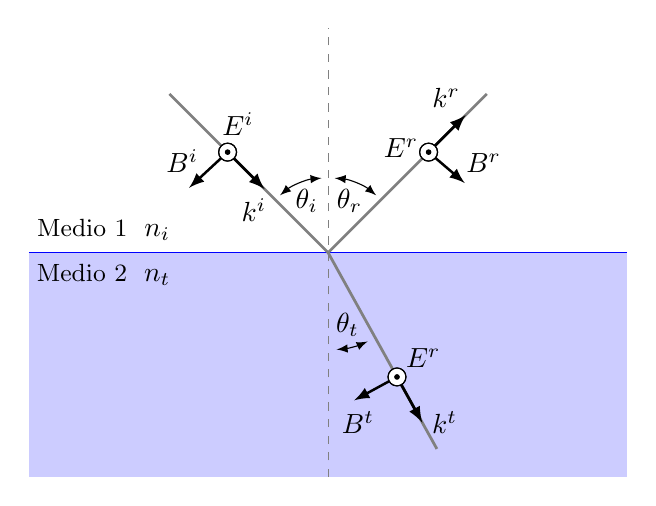
\begin{tikzpicture}[scale=.95]

%-------------------------------------------- Incidence media
\fill[blue!20] (-4,-3) rectangle (4,0);
% Interface
\draw[blue,line width=.5pt](-4,0)--(4,0); %%..5pt, interface]
% Vertical dashed line
\draw[dashed,gray,](0,-3)--(0,3);
% Media names
\node at (-3,.3) {{\small Medio 1} $\; n_i$}; 
\node at (-3,-.3) {{\small Medio 2} $\; n_t$};

%--------------------------------------------  Incident Wave
\draw[gray, line width=1pt](0:0cm)--(135:3cm);  % Light trajectory
\path (0,0)++(112.5:.75cm)node{$\theta_i$};       % Angle
\draw[latex-latex](95:1.cm)arc(95:130:1.cm);
 
    \draw[-latex,line width=1pt](135:1.9cm)--(135:1.2cm);    %Wave vector
    \path (0,0)++(141:0.9cm)node[left]{$\vb{k}^i$};     %Wave vector label
    
    \draw[-latex,line width=.9pt](135:1.9cm)--(155:2.05cm);  %B vector
    \path (0,0)++(148:2.3cm)node{$\vb{B}^i$}; 
    
    \path (0,0)++(125:2.1cm)node{$\vb{E}^i$};       % E vector
    
    \draw [fill= white](135:1.9cm)circle (0.12cm); % Vector perp. to surface
    \draw [black](135:1.9cm)circle (0.12cm);
    \filldraw[fill=black](135:1.9cm) circle(0.03cm); %%
    
%--------------------------------------------  Reflected Wave
\draw[gray,line width=1pt](0:0cm)--(45:3cm);  % Light trajectory
\path (0,0)++(67.5:.75cm)node{$\theta_r$};       % Angle
\draw[latex-latex](85:1.cm)arc(85:50:1.cm);
 
    \draw[-latex,line width=1pt](45:1.9cm)--(45:2.6cm);    %Wave vector
    \path (0,0)++(47.5:2.8cm)node[left]{$\vb{k}^r$};     %Wave vector label
    
    \draw[-latex,line width=.9pt](45:1.9cm)--(27:2.05cm);  %B vector
    \path (0,0)++(30:2.4cm)node{$\vb{B}^r$}; 
    
    \path (0,0)++(55:1.7cm)node{$\vb{E}^r$};       % E vector
    
    \draw [fill= white](45:1.9cm)circle (0.12cm); % Vector perp. to surface
    \draw [black](45:1.9cm)circle (0.12cm);
    \filldraw[fill=black](45:1.9cm) circle(0.03cm); %%

%--------------------------------------------  Transmitted Wave
\draw[gray,line width=1pt](0:0cm)--(-61:3cm);  % Light trajectory
\path (0,0)++(-75:1cm)node{$\theta_t$};       % Angle
\draw[latex-latex](-85:1.3cm)arc(-85:-66:1.3cm);
 
    \draw[-latex,line width=1pt](-61:1.9cm)--(-61:2.6cm);    %Wave vector
    \path (0,0)++(-61:2.6cm)node[right]{$\vb{k}^t$};     %Wave vector label

    \draw[-latex,line width=.9pt](-61:1.9cm)--(-80:2.005cm);  %B vector
    \path (0,0)++(-80:2.3cm)node{$\vb{B}^t$}; 
    
    \path (0,0)++(-48:1.9cm)node{$\vb{E}^r$};       % E vector
    
    \draw [fill= white](-61:1.9cm)circle (0.12cm); % Vector perp. to surface
    \draw [black](-61:1.9cm)circle (0.12cm);
    \filldraw[fill=black](-61:1.9cm) circle(0.03cm); %%     
 
\end{tikzpicture}
	\end{subfigure}
	\begin{subfigure}{.05\textwidth}\vspace{-4.5cm}\caption{}\label{sfig:Polp}	\end{subfigure}
	\begin{subfigure}{.43\textwidth}  \hspace*{-1cm}
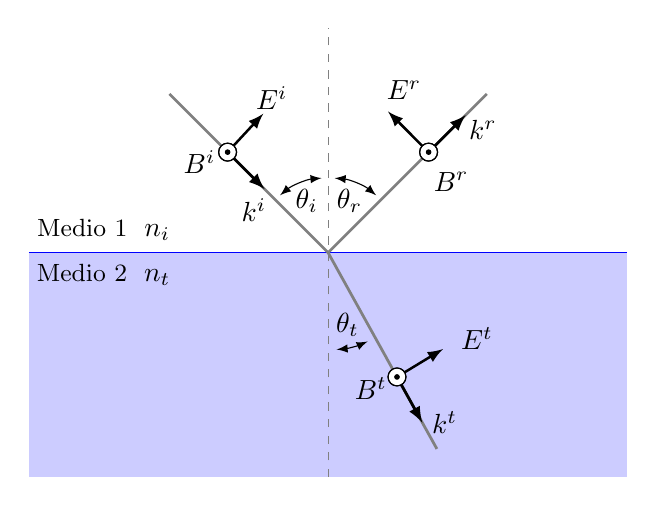
\begin{tikzpicture}[scale=.95]
%-------------------------------------------- Incidence media
\fill[blue!20] (-4,-3) rectangle (4,0);
% Interface
\draw[blue,line width=.5pt](-4,0)--(4,0); %%..5pt, interface]
% Vertical dashed line
\draw[dashed,gray,](0,-3)--(0,3);
% Media names
\node at (-3,.3) {{\small Medio 1} $\; n_i$}; 
\node at (-3,-.3) {{\small Medio 2} $\; n_t$};

%--------------------------------------------  Incident Wave
\draw[gray, line width=1pt](0:0cm)--(135:3cm);  % Light trajectory
\path (0,0)++(112.5:.75cm)node{$\theta_i$};       % Angle
\draw[latex-latex](95:1.cm)arc(95:130:1.cm);
 
    \draw[-latex,line width=1pt](135:1.9cm)--(135:1.2cm);    %Wave vector
    \path (0,0)++(141:0.9cm)node[left]{$\vb{k}^i$};     %Wave vector label
    
    \draw[-latex,line width=.9pt](135:1.9cm)--(115:2.05cm);  %E vector
    \path (0,0)++(110:2.2cm)node{$\vb{E}^i$}; 
%    \draw[-latex,line width=.9pt, red]((135:1.9cm)--(117:1.55cm); 

    
    \path (0,0)++(145:2.1cm)node{$\vb{B}^i$};       % B vector
    
    \draw [fill= white](135:1.9cm)circle (0.12cm);
    \draw [black](135:1.9cm)circle (0.12cm);
    \filldraw[fill=black](135:1.9cm) circle(0.03cm); %%    
    
    
%    \draw[line width=.6pt] (135:1.9cm)   % Esto esra paea hacer el vector salir de la hoja
%                         +(-135:.12cm) -- +(45:.12cm)
%                         +(-45:.12cm) -- +(135:.12cm);    
   
    
%--------------------------------------------  Reflected Wave
\draw[gray,line width=1pt](0:0cm)--(45:3cm);  % Light trajectory
\path (0,0)++(67.5:.75cm)node{$\theta_r$};       % Angle
\draw[latex-latex](85:1.cm)arc(85:50:1.cm);
 
    \draw[-latex,line width=1pt](45:1.9cm)--(45:2.6cm);    %Wave vector
    \path (0,0)++(43:2.4cm)node[right]{$\vb{k}^r$};     %Wave vector label
    
    \draw[-latex,line width=.9pt](45:1.9cm)--(67:2.05cm);  %E vector
    \path (0,0)++(65:2.4cm)node{$\vb{E}^r$};
  %  \draw[-latex,line width=.9pt, red](45:1.9cm)--(59:1.55cm); 
   % \draw[dashed,red,line width=.9pt](59:1.55cm)--(67:2.05cm);
    
    \path (0,0)++(30:1.9cm)node{$\vb{B}^r$};       % B vector
    
    \draw [fill= white](45:1.9cm)circle (0.12cm);
    \draw [black](45:1.9cm)circle (0.12cm);
    \filldraw[fill=black](45:1.9cm) circle(0.03cm); %%  


%--------------------------------------------  Transmitted Wave
\draw[gray,line width=1pt](0:0cm)--(-61:3cm);  % Light trajectory
\path (0,0)++(-75:1cm)node{$\theta_t$};       % Angle
\draw[latex-latex](-85:1.3cm)arc(-85:-66:1.3cm);
 
    \draw[-latex,line width=1pt](-61:1.9cm)--(-61:2.6cm);    %Wave vector
    \path (0,0)++(-61:2.6cm)node[right]{$\vb{k}^t$};     %Wave vector label
 
    \draw[-latex,line width=.9pt](-61:1.9cm)--(-40:2.005cm);  %E vector
%      \draw[-latex,line width=.9pt, red](-61:1.9cm)--(-45:2.3cm); 
    \path (0,0)++(-30:2.3cm)node{$\vb{E}^t$}; 
    
    \path (0,0)++(-72.5:1.9cm)node{$\vb{B}^t$};       % B vector
    
    \draw [fill= white](-61:1.9cm)circle (0.12cm);
    \draw [black](-61:1.9cm)circle (0.12cm);
    \filldraw[fill=black](-61:1.9cm) circle(0.03cm); %% 
\end{tikzpicture}
	\end{subfigure} 
	\caption{ Esquema de una onda plana en polarización \textbf{a)} \emph{s} y \textbf{b)} \emph{p} que se propaga en una dirección $\vb{k}^i$ e incide con un ángulo de incidencia $\theta_i$ sobre una interfaz plana entre dos medio lineales, homogéneos e isótropos, donde el medio de incidencia tiene un índice de refracción $n_i$ y el de transmisión $n_t$. El vector de onda reflejado forma un ángulo $\theta_r=\theta_i$ con la dirección normal a la intrfaz, dado por la ley de reflexión [Ec. \eqref{eq:LeyReflexion}] y el vector de onda transmitido se propaga con un ángulo $\theta_t$ dado por la ley de Snell [Ec. \eqref{eq:LeySnell}]. En el esquema se asume que la orientación de los campos EMs incidentes  ($\vb{E}^i,\,\vb{B}^i$) se preserva en los campos EMs reflejados ($\vb{E}^r,\,\vb{B}^r$) y transmitidos ($\vb{E}^t,\,\vb{B}^t$), es decir, que no hay un cambio de fase de los campos EMs al interactuar con la interfaz.}	\label{fig:Polarizaciones}	
	\end{figure}	
%

En polarización \emph{s} el campo eléctrico es perpendicular al plano de incidencia y paralelo a la interfaz por lo que, mediante la Ec. \eqref{seq:Epara}, $E^i + E^r = E^t$, en donde se asume que la orientación del campo eléctrico incidente se preserva tras la reflexión y la transmisión, como se observa en la Fig. \ref{sfig:Pols}. Al emplear la continuidad de la componente paralela a la interfaz de $\vb{B}/\mu$ [Ec. \eqref{seq:Bpara}], la relación $E = (c/n) B$, la ley de la reflexión [Ec. \eqref{eq:LeyReflexion}] y de Snell [Ec. \eqref{eq:LeySnell}], así como considerar medios no magnéticos ($\mu=\mu_0$), se obtienen los coeficientes de amplitud $r$ y $t$ para  polarización \emph{s}, dados por \cite{hecht1998optics}\vspace{-.5em}
%
	\begin{tcolorbox}[title = Coeficientes de amplitud para polarización \emph{s} ]
	\vspace*{-1em}	
	\eqhalf{r_s =
		\frac{n_i\cos\theta_i-\sqrt{n_t^2-n_i^2\sin ^2\theta_i}}
 			{n_i \cos\theta_i + \sqrt{ n_t^2-n_i^2\sin ^2\theta_i}}, 
 			\label{eq:rs}}
	\eqhalf{ t_s =
		\frac{2n_i\cos\theta_i}
 			{n_i\cos\theta_i + \sqrt{ n_t^2-n_i^2\sin ^2\theta_i}}.
 			\label{eq:ts}}
	\end{tcolorbox}	 \vspace*{-.75em}\noindent
%
Para polarización \emph{p} el campo eléctrico es paralelo al plano de incidencia, y por tanto tiene una componente paralela y una perpendicular a la interfaz, como se observa en la Fig. \ref{sfig:Polp}. Las condiciones a la frontera de los campos EM [Ec. \eqref{seq:Epara}] imponen que $E^i\cos\theta_i-E^r\cos\theta_r = E^t \cos\theta_t$. Al asumir que los campos EMs reflejado y transmitido no tienen una fase respecto a los campos EMs incidentes, y al emplear las Ecs. \eqref{seq:Bpara},  \eqref{eq:LeyReflexion} y  \eqref{eq:LeySnell}, así como la relación $E = (c/n) B$ y considerar medios no magnéticos, se calculan los  coeficientes de amplitud $r$ y $t$ para  polarización \emph{p} dados por \cite{hecht1998optics}\vspace*{-.75em}
%
	\begin{tcolorbox}[title = Coeficientes de amplitud para polarización \emph{p} ]
	\vspace*{-1em}
	\eqhalf{ r_p =
				\frac{n_t^2\cos\theta_i -n_i\sqrt{n_t^2-n_i^2\sin^2\theta_i}}
 				{n_t^2\cos\theta_i +n_i\sqrt{n_t^2-n_i^2\sin^2\theta_i}}, \label{eq:rp}}
	\eqhalf{ t_p =
				\frac{ 2 n_i n_t \cos\theta_i}
 				{n_t^2\cos \theta_i+n_i\sqrt{n_t^2-n_i^2\sin^2\theta_i}}.
 				\label{eq:tp}}
	\end{tcolorbox}	\vspace*{-.75em}\noindent
%
Dado que los coeficientes  de amplitud dependen de los índices de refracción de los medios que conforman la interfaz, es posible hacer la distinción entre dos casos al analizar el término dentro de la raíz cuadrada en las Ecs. \eqref{eq:rs}--\eqref{eq:tp}: incidencia externa ($n_t>n_i$) e incidencia interna ($n_t<n_i$). En la Fig. \ref{fig:coefAmp} se grafican los coeficientes de amplitud $r$ (líneas continuas) y $t$ (líneas discontinuas) en función del ángulo de incidencia $\theta_i$ para una interfaz entre aire ($n= 1$) y un medio con un índice de refracción $n = 1.5$, en configuración de incidencia externa [Fig. \ref{sfig:coefExt}] e interna [Fig. \ref{sfig:coefInt}] para ambas polarizaciones, en donde las líneas azules corresponden a la polarización \emph{s} y las rojas a \emph{p}. PAra el caso de incidencia interna $n_t<n_i$ los coeficientes de amplitud son cantidades complejas, por lo que se grafica tanto su parte real como la imaginaria en la Fig. \ref{sfig:coefInt}.\index{Incidencia!interna}\index{Incidencia!externa}
%
\begin{figure}[h!]\centering\hspace*{-1.5em}
	\begin{subfigure}{.05\textwidth}\vspace{-4.5cm}\caption{}\label{sfig:coefExt}\end{subfigure}
	\begin{subfigure}{.43\textwidth} \hspace*{-.8cm}
	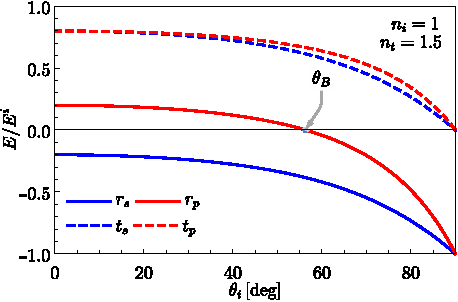
\includegraphics[scale=1]{1-Teoria/figs/1-1-ampCoefExt}
	\end{subfigure}
	\begin{subfigure}{.05\textwidth}\vspace{-4.5cm}\caption{}\label{sfig:coefInt}\end{subfigure}
	\begin{subfigure}{.43\textwidth} \hspace*{-.9cm}
	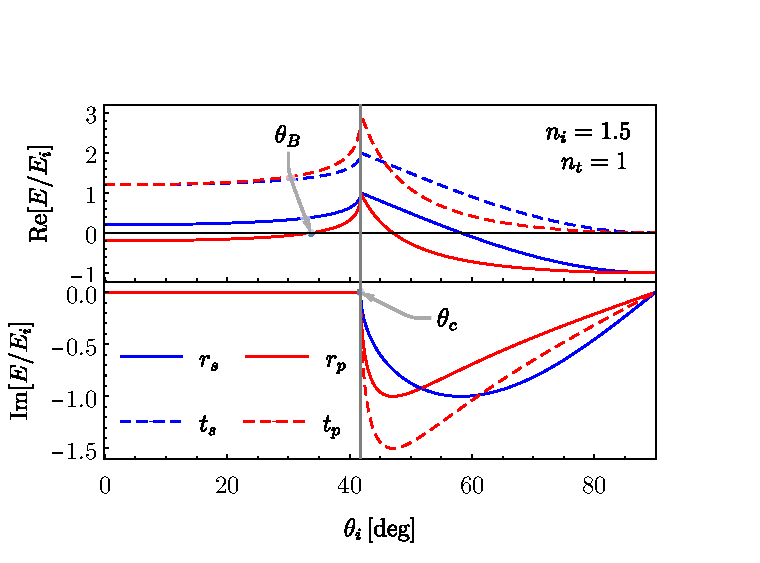
\includegraphics[scale=1]{1-Teoria/figs/1-1-ampCoefInt}
	\end{subfigure}\vspace*{-.7em}
	\caption{ Coeficientes de amplitud $r$ (líneas continuas) y $t$ (líneas discontinuas), en función del ángulo de incidencia $\theta_i$, en configuración de incidencia \textbf{a)} externa e \textbf{b)} interna para una interfaz entre  aire ($n=1$) y un medio con índice de refracción $n = 1.5$. Los cálculos para polarización  \emph{s} se muestran  en azul y  para \emph{p} en rojo; en el caso de incidencia interna, los coeficientes de amplitud son cantidades complejas y se grafica tanto su parte real, como la imaginaria. Se indica la posición tanto el ángulo de Brewster $\theta_B$ como el ángulo crítico $\theta_c$ mediante las flechas grises.}	\label{fig:coefAmp}	
	\end{figure}	

En la Fig. \ref{fig:coefAmp}, se muestran dos valores partículares para el ángulo de incidencia. Uno de ellos es el  ángulo Brewster $\theta_B$, valor al que el coeficiente de amplitud de reflexión $r_p$ [Ec. \eqref{eq:rp}] es igual a cero. El ángulo de Brewster está dado por \cite{hecht1998optics}\index{Ángulo!de Brewster} \index{Brewster!ángulo de}
%
	\begin{align}
	\tan\theta_B = \frac{n_t}{n_i},
	\label{eq:Brewster}
	\end{align}
%	
tanto para incidencia externa [Fig. \ref{sfig:coefExt}], donde $\theta_B \approx 56^\circ$, como para interna [Fig. \ref{sfig:coefInt}], donde $\theta_B \approx 33^\circ$. El cambio de signo del coeficiente de reflexión $r_p$ para $\theta_i>\theta_B$ corresponde a un cambio de fase de $\pi$ radianes del campo eléctrico reflejado respecto al campo eléctrico incidente. De la Ec. \eqref{eq:Brewster} se deduce que el ángulo de Brewster de incidencia externa $\theta_B^{ext}$ es complementario al de incidencia interna $\theta_B^{int}$, es decir, $\theta_B^{ext}+\theta_B^{int} = 90^\circ$, como se observa en las gráficas de la Fig. \ref{fig:coefAmp}. Un segundo valor particular para el ángulo de incidencia es el ángulo crítico $\theta_c$, el cual se observa sólo en incidencia interna ($n_i>n_t$)  y  cumple la expresión \cite{hecht1998optics}\index{Ángulo!crítico|see {Incidencia interna}}\index{Ángulo!crítico}
% 
	\begin{align}
	\sin\theta_c = \frac{n_t}{n_i}.
	\label{eq:Criticp}
	\end{align}
%
Al evaluar los coeficientes de amplitud  [Ecs. \eqref{eq:rs}--\eqref{eq:tp}] en ángulo mayores a $\theta_c$, estos son cantidades complejas. Adicionalmente, al sustituir la Ec. \eqref{eq:Criticp} en la ley de Snell [Ec. \eqref{eq:LeySnell}] se obtiene que $\theta_t = 90^\circ$, por lo que para $\theta_i>\theta_c$ toda la luz se refleja (nada se transmite), es decir, se está en el régimen de \emph{reflexión total interna} \index{Reflexión total!interna}. En la Fig. \ref{sfig:coefInt} se observa que los coeficientes de amplitud son máximos en $\theta_c \approx 41^\circ$ sin embargo, para $\theta_i>\theta_c$, los coeficientes de amplitud  [Ecs. \eqref{eq:rs}--\eqref{eq:tp}] son cantidades complejas, lo que indica que los campos eléctricos reflejado y transmitido tienen un desfase, distinto de $\pi$ radianes, respecto al campo eléctrico incidente.  

Para corroborar que toda la luz es reflejada en incidencia interna para $\theta_i>\theta_c$ se considera la conservación de la energía transportada por los campos EMs al cruzar la interfaz. Al calcular el promedio temporal\footnote{El promedio temporal del vector de Poynting es $\langle\vb{S}\rangle_t = (1/\tau)\int_t^{t+\tau}\vb{S}(t')dt'$, y para campos EMs tipo ondas planas es $\langle\vb{S}\rangle_t = (1/2) \Re[\vb{E}\times\qty(\vb{B}/\mu)^*]$ \cite{jackson1999electrodynamics}.\index{Poynting!vector de!promedio temporal del}}, del vector de Poynting [Ec. (\ref{eq:Poynting})], se obtiene la irradiancia $I$ \cite{hecht1998optics}, dada por
	\begin{align}
	I = \langle S \rangle_t = \frac{nc\varepsilon_0}{2} EE^*,
	\label{eq:Irr}
	\end{align}
que corresponde a la energía promedio por unidad de tiempo y unidad de área  transportada por los campos EMs en la dirección $\vu{k}$ \cite{griffiths2013electrodynamics}. Para calcular la potencia $P$, definida como energía por unidad de tiempo, transportada por los campos EMs al cruzar la interfaz se multiplica la Ec. \eqref{eq:Irr} por la sección transversal de un haz de luz. En la Fig. \ref{fig:hazcircular} se muestran las secciones transversales de un haz  que incide a un ángulo $\theta_i$ sobre la interfaz entre dos medios con índice de refracción $n_i$ y $n_t$, respectivamente. Cuando el haz se refleja, a un ángulo $\theta_r=\theta_i$, y se refracta a un ángulo $\theta_t$, la sección transversal del haz cambia. Si el área de los haces justo en la interfaz es $A$, mediante la ley de la reflexión [Ec. \eqref{eq:LeyReflexion}] y la ley de Snell [Ec. \eqref{eq:LeySnell}], la sección transversal del haz incidente y el reflejado  es $A\cos\theta_i$, mientras que la del haz transmitido es $A\cos\theta_t$. Al emplear la Ec. \eqref{eq:Irr} y multiplicarla por el área de cada uno de los tres haces mostrados en la Fig. \ref{fig:hazcircular}, se obtiene que la energía por unidad de tiempo transportada por cada haz de luz es
	\begin{align*}
	P = I A \cos\theta = \frac{n c \varepsilon_0}{2}  EE^* \cos\theta,
	\end{align*}
en donde el ángulo $\theta$ e índice de refracción $n$ toman los valores de $\theta_i$ y $n_i$ para el haz incidente y el reflejado, mientras que  toma los valores de $\theta_t$ y  $n_t$ para el haz transmitido. Cuando se normaliza la energía por unidad de tiempo transportada por el haz reflejado y por el haz transmitido, entre la del haz incidente se obtienen las expresiones de la reflectancia $R$ y la transmitancia $T$ \cite{hecht1998optics} \vspace{-.5em} \index{Fresnel!Reflectancia ($R$)}\index{Fresnel!Transmitancia ($T$)}
	\begin{tcolorbox}[title = Reflectancia y transmitancia]
	\eqhalf{ R =  r r^*, \label{eq:R}}
	\eqhalf{ T = \frac{n_t\cos\theta_i}{n_i \cos\theta_t} t t^*,\label{eq:T}}
	\end{tcolorbox}\vspace*{-.75em}\noindent	
en donde $r$ es el coeficiente de amplitud de reflexión y $t$ el de transmisión, dados por las Ecs. \eqref{eq:rs}--\eqref{eq:tp}.

	\begin{figure}[t]\centering
\begin{tikzpicture}[scale=.7]
%\draw (3.46,1.9) circle(2pt);ESTA ES LAREFERENCIA PARA ANTES DE MOVER LAS COSAS

%---------------------------------------------------------------------------------------- SUPERFICIE
\fill[blue!20]			
(-5,-1) -- (-3,2) 
-- (3,2) -- (5,-1)
--(-5,-1);						

\draw[dashed,gray](0,-4)--(0,5);  %---------------------------------------------------- Vertical dashed line

\node at (-4,-.5) {Medio 1 $\; n_i$}; %-------------------------------------------------- media names
\node at (-4,-1.5) {Medio 2 $\; n_t$};

%---------------------------------------------------------------------------------------- SPOT INTERFAZ
\fill[lgreen, opacity= .75] (0,.5) circle (2 and .6); 
\draw[black](0,.5) circle (2 and .6)		% -------------------------------------------  Etiqueta área
			(0,.5)node[]{$A$};	
%------------------------------------------------------------- INCIDENTE
\path[shift = {(0,1.7)}] (0,0)++(112.5:1cm)node{$\theta_i$};   %---------- Angle
\draw[latex - latex,shift = {(0,2.1)}](-1,.5)arc(144.5:90:1.1cm);

\draw [-,shift = {(-2,.5)}, rotate = 55.5] (0,0) -- (0,3.2);%Cara del cilindro(Rota desde 90°)
\draw[-, shift = {(2,.5)},rotate = 55.5] (0,0) -- (0,6.3);

\draw[black, rotate = 50.75, shift = {(0,5)}](0,0) circle (1.145 and .3);% Tapa del cilidndro del del área
\node at (-5.1,3.5) { $A\cos\theta_i$};
\fill[lgreen, opacity= .5, rotate = 50.75, shift = {(0,5)}](0,0) circle (1.145 and .3);

%-------------------------------------------------------------- REFLEJADO
\path[shift = {(0,1.7)}] (0,0)++(67.5:1cm)node{$\theta_r$};   %------------- Angle
\draw[latex - latex ,shift = {(0,2.1)}](1,.5)arc(35:90:1.1cm);

\draw [-,shift = {(-2,.5)}, rotate = -55.5] (0,0) -- (0,6.3);  %- Cara del cilindro
\draw[-, shift = {(2,.5)},rotate = -55.5] (0,0) -- (0,3.2);

\draw[black, rotate = -50.75, shift = {(0,5)}](0,0) circle (1.145 and .3); %Tapa del cilidndro del del área
\node at (5.1,3.5) { $A\cos\theta_r$};
\fill[lgreen , opacity= .5, rotate = -50.75, shift = {(0,5)}](0,0) circle (1.145 and .3);

%----------------------------------------------------------------- TRANSMITIDO
\path  (0,0)++(275:4.1)node{$\theta_t$};    %------------------------- Angle
\draw[latex - latex](0,-3.5)arc(270:290:1.5cm);

\draw [-,shift = {(-2,.5)}, rotate = 33.5] (0,0) -- (0,-5);   %------------------------- Cara del cilindro
\draw[-, shift = {(2,.5)},rotate = 33.5] (0,0) -- (0,-3.1);

\draw[black, rotate = 29.2, shift = {(.5,-3.6)}](0,0) circle (1.675 and .3);		%-------- Tapa del cilidndro del del área
\node at (3.5,-3.5) {$A\cos\theta_t$};
\fill[lgreen, opacity= .5,  rotate = 29.2, shift = {(.5,-3.6)}](0,0) circle (1.675 and .3);

\end{tikzpicture}
	\caption{Sección transversal de un haz de luz incidiendo en una interfaz entre dos medio lineales, homogéneos e isótropos con índices de refracción $n_i$ y $n_t$. El haz incide sobre la interfaz a un ángulo de $\theta_i$, se refleja con un ángulo $\theta_r$ y se transmite a un ángulo $\theta_t$, calculados mediante las leyes de la reflexión y de Snell, respectivamente. El área del haz sobre la interfaz es $A$, mientras que en los haces, al propagarse, es $A\cos\theta$, en donde $\theta$ es el ángulo de propagación respectivo para cada haz.} \label{fig:hazcircular}
	\end{figure}

En la Fig. \ref{fig:frsnel} se grafican la reflectancia (líneas continuas) y transmitancia (líneas discontinuas) en función del ángulo de incidencia $\theta_i$, para la polarización \emph{s} (en azul) y \emph{p} (en rojo), de un haz de luz que incide en la interfaz entre aire ($n=1$) y un medio con índice de refracción $n=1.5$, para una configuración de incidencia externa [Fig. \ref{sfig:frsnelExt}] e incidencia interna [Fig. \ref{sfig:frsenlInt}]. En la Fig. \ref{fig:frsnel} se observa que $R_p=0$ para el ángulo de Brewster, tanto para incidencia interna como externa. Asimismo, se aprecia que la relación $R+T=1$ se cumple para todo ángulo de incidencia y en particular para $\theta_i>\theta_c$ se cumple que $R_p = R_s = 1$ y que $T_s = T_p = 0$. La relación $R+T=1$ es válida ya que se consideraron medios materiales sin absorción. En general, la función dieléctrica ($\sqrt{\epsilon}=n^2$ para medios no magnéticos) es compleja, donde la parte su parte imaginaria   $\Im[\varepsilon]$ se asocia con la absorción de energía por el material \cite{ibach2003solid}. Cuando la luz se propaga a través de algún medio absorbente, se cumple en general 
	\begin{align*}
	R + T + A = 1,
	\end{align*}
en donde el término $A$ es la energía absorbida por el material, relativa a la energía del haz incidente.\index{Función dieléctrica!Absorción}
%
\begin{figure}[t!]\centering\hspace*{-1.5em}
	\begin{subfigure}{.05\textwidth}\vspace{-4.5cm}\caption{}\label{sfig:frsnelExt}\end{subfigure}
	\begin{subfigure}{.43\textwidth} \hspace*{-.7cm}
	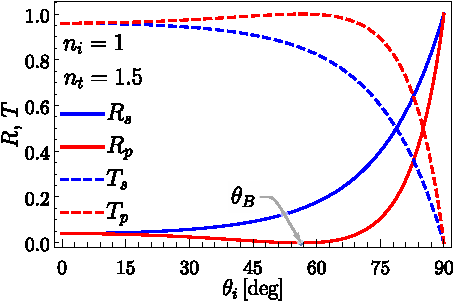
\includegraphics[scale=1]{1-Teoria/figs/1-2-FrsnelExt}
	\end{subfigure}
	\begin{subfigure}{.05\textwidth}\vspace{-4.5cm}\caption{}\label{sfig:frsenlInt}\end{subfigure}
	\begin{subfigure}{.43\textwidth} \hspace*{-.7cm}
	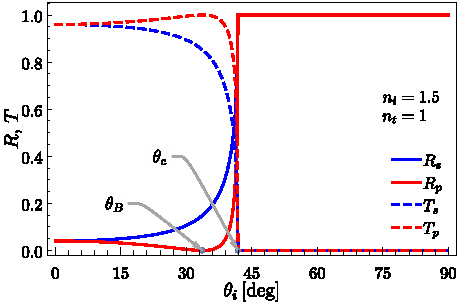
\includegraphics[scale=1]{1-Teoria/figs/1-2-FrsnelInt}
	\end{subfigure}\vspace*{-.7em}
	\caption{  Reflectancia (líneas continuas) y transmitancia (líneas discontinuas), en función del ángulo de incidencia $\theta_i$, en configuración de incidencia \textbf{a)} externa e \textbf{b)} interna para una interfaz entre  aire ($n=1$) y un medio con índice de refracción $n = 1.5$. Los cálculos para polarización  \emph{s} se muestran  en azul y  para \emph{p} en rojo. Se indica la posición tanto el ángulo de Brewster $\theta_B$, como el ángulo crítico $\theta_c$ mediante las flechas grises.}	\label{fig:frsnel}	
	\end{figure}	
%
	% !TeX root = ../tesis.tex

\section{Solución de Mie}
\label{section:Mie}

\index{Mie!solución de}\index{Esparcimiento! de luz|see{Mie}}
El problema de absorción y esparcimiento de luz por una partícula esférica de tamaño arbitrario fue resuelto por el físico alemán Gustav Mie en 1908 \cite{mie1908metallosung}. La solución de Mie consiste en expandir una onda plana monocromática, que ilumina a una esfera de tamaño y material arbitrario, en una base de armónicos esféricos vectoriales que representan una base ortogonal, cuyos elementos satisfacen las ecuaciones de Maxwell \cite{bohren1998absorption}. Al considerar las condiciones de contorno que satisfacen los campos EMs sobre la superficie de la esfera, se escriben los campos EMs dentro de la partícula y los campos esparcidos por ésta como una serie de armónicos esféricos vectoriales, cuyos coeficientes corresponden a una expansión multipolar y son conocidos como los coeficientes de Mie \cite{bohren1998absorption}. A pesar de que existen publicaciones previas a la de Mie en donde  el problema de la absorción y esparcimiento de luz es tratado de forma semejante, el trabajo de Mie destacó debido al desarrollo de relaciones recursivas que facilitan el cálculo numérico y a que discute la convergencia de los resultados \cite{horvath2009historic}. El desarrollo de una solución apta para el cálculo numérico permitió que en el artículo de Mie se describieran diez propiedades de la luz al interactuar con suspensiones diluidas de partículas esféricas \cite{mie1908metallosung}, lo que contribuyó al impacto de su solución sobre el trabajo de otros autores \cite{horvath2009historic}. El desarrollo de la solución de Mie descrito en esta sección se basa principalmente en \cite{bohren1998absorption}.

	\begin{figure}[h!]\centering
	\tdplotsetmaincoords{60}{110}
	\pgfmathsetmacro{\rvec}{1. 3}
	\pgfmathsetmacro{\thetavec}{30}
	\pgfmathsetmacro{\varphivec}{60}
\begin{tikzpicture}[scale=3.5,tdplot_main_coords]
%draw the NP
	\draw[tdplot_screen_coords,ball color=yellow, opacity = 1] (0,0,0) circle (.05);
	\draw[tdplot_screen_coords, color=yellow, opacity = 1] (0,0,0) circle (.05);


%set up some coordinates 
	\coordinate (O) at (0,0,0);

%determine a coordinate (P) using (r,\theta,\varphi) coordinates.   This command
%also determines (Pxy), (Pxz), and (Pyz): the xy-, xz-, and yz-projections
%of the point (P). 
%syntax: \tdplotsetcoord{Coordinate name without parentheses}{r}{\theta}{\varphi}
	\tdplotsetcoord{P}{\rvec}{\thetavec}{\varphivec}

%draw figure contents
%--------------------
%draw the main coordinate system axes
	\draw[thick,- latex] (0,0,0) -- (1. 5,0,0) node[anchor=north east]{$x$};
	\draw[thick,- latex] (0,0,0) -- (0,1. 5,0) node[anchor=north west]{$y$};
	\draw[thick,- latex] (0,0,0) -- (0,0,1. 5) node[anchor=south]{$z$};

%draw the main cartesian vector system 
	\draw[thick,- latex, blue] (0,0,0) -- (1,0,0) node[anchor= south east]{$\vu{e}_x$};
	\draw[thick,- latex, blue] (0,0,0) -- (0,1,0) node[anchor=north west]{$\vu{e}_y$};
	\draw[thick,- latex, blue] (0,0,0) -- (0,0,1) node[anchor= east]{$\vu{e}_z$};

%draw a vector from origin to point (P) 
	\draw[thick,color=green, - latex] (O) -- (P);
	\node at (1,. 5,1. 1) {\color{green} $\vb{r}$};

%draw projection on xy plane, and a connecting line
	\draw[dashed, color=green] (O) -- (Pxy);
	\draw[dashed, color=green] (P) -- (Pxy);
	\fill[green, opacity = .3] (O) --(Pxy)-- (P)--(O);
	\draw[- latex, tdplot_screen_coords,green](.42,.2)--(.8,.2);
	\node[tdplot_screen_coords] at (1.35,.2) {\color{green}\small Plano de esparcimiento};


%draw the angle \varphi, and label it
	%syntax: \tdplotdrawarc[coordinate frame, draw options]{center point}{r}{angle}{label options}{label}
	\tdplotdrawarc[- latex]{(O)}{0. 5}{0}{\varphivec}{anchor=south}{$\varphi$}


%set the rotated coordinate system so the x'-y' plane lies within the
	%"theta plane" of the main coordinate system
	%syntax: \tdplotsetthetaplanecoords{\varphi}
	\tdplotsetthetaplanecoords{\varphivec}

%draw theta arc and label, using rotated coordinate system
	\tdplotdrawarc[tdplot_rotated_coords, - latex]{(0,0,0)}{0. 45}{0}{\thetavec}{anchor=north}{$\theta$}

%draw some dashed arcs, demonstrating direct arc drawing
	\draw[dashed,tdplot_rotated_coords] (\rvec,0,0) arc (0:90:\rvec);
	\draw[dashed] (\rvec,0,0) arc (0:90:\rvec);

%set the rotated coordinate definition within display using a translation
%coordinate and Euler angles in the "z(\alpha)y(\beta)z(\gamma)" euler rotation convention
%syntax: \tdplotsetrotatedcoords{\alpha}{\beta}{\gamma}
	\tdplotsetrotatedcoords{\varphivec}{\thetavec}{0}

%translate the rotated coordinate system
%syntax: \tdplotsetrotatedcoordsorigin{point}
	\tdplotsetrotatedcoordsorigin{(P)}

%use the tdplot_rotated_coords style to work in the rotated, translated coordinate frame
	\draw[thick,tdplot_rotated_coords,- latex, purple] (0,0,0) -- (. 3,0,0) node[anchor=north west]{{\color{black}$\vu{e}_\theta,$}$\vu{e}_{\parallel}^s$};
	\draw[thick,tdplot_rotated_coords,- latex,black] (0,0,0) -- (0,. 3,0) node[anchor=west]{$\vu{e}_\varphi$};
	\draw[thick,tdplot_rotated_coords,- latex,purple] (0,0,0) -- (0,-. 3,0) node[anchor= north west]{$\vu{e}_{\perp}^s$};
	\draw[thick,tdplot_rotated_coords,- latex] (0,0,0) -- (0,0,. 3) node[anchor=south]{$\vu{e}_r$ };



%set the rotated coordinate definition within display using a translation
%coordinate and Euler angles in the "z(\alpha)y(\beta)z(\gamma)" euler rotation convention
%syntax: \tdplotsetrotatedcoords{\alpha}{\beta}{\gamma}
	\tdplotsetrotatedcoords{\varphivec}{0}{0}

%translate the rotated coordinate system
%syntax: \tdplotsetrotatedcoordsorigin{point}
	\tdplotsetrotatedcoordsorigin{(Pxy)}

	\draw[thick,tdplot_rotated_coords,- latex, purple] (0,0,0) -- (. 3,0,0) node[anchor= west]{$\vu{e}_{\parallel}^i$};
	\draw[thick,tdplot_rotated_coords,- latex, blue] (0,0,0) -- (0,0,. 3) node[anchor= west]{$\vu{e}_z$};	
	\draw[thick,tdplot_rotated_coords,- latex, purple] (0,0,0) -- (0,-. 3,0) node[anchor= north west]{$\vu{e}_{\perp}^i$};



% Plane Wave
	\foreach \i in {-7,...,-2}{
		\draw[thick,tdplot_screen_coords,red, - latex] (\i/10,0,0)--(\i/10,1,0);}
	\node[tdplot_screen_coords] at (-4.5/10,1.1,0){\color{red}$\vb{k}_i$};
	\node[tdplot_screen_coords] at (-4.5/10,-.1,0){\small \color{red}Haz incidente};
\end{tikzpicture}
%
\caption{Diagrama del plano de esparcimiento (en verde) definido por el vector $\vb{r}$, posición donde se evalúan los campos EMs, y el vector $\vu{e}_z$, cuando una onda plana monocromática propagándose en dirección $z$ (en rojo) ilumina a una partícula arbitraria.  La base cartesiana para vectores se muestra en azul, mientras que la base esférica se muestra en negro.  Las direcciones paralelas $\parallel$ y perpendiculares $\perp$ al plano de incidencia  para el campo eléctrico incidente, denotado por el subíndice $i$ y el esparcido, denotado por el subíndice $s$, se muestran en morado; el haz incidente se muestra en rojo.}\label{fig:PlanoEsparcimiento}
	\end{figure}	

Para  el estudio del esparcimiento por una partícula arbitraria inmersa en un medio con índice de refracción $n_m$, denominado  matriz, se considera que la partícula es iluminada por una onda plana monocromática con una longitud de onda $\lambda$, cuya dirección de propagación define la dirección $z$, es decir,
	\begin{align}
	\vb{E}^i = (E_x^i \vu{e}_x + E_y^i \vu{e}_y)e^{i(k z - \omega t)},
	\label{eq:Exyi}
	\end{align}
donde $k = 2\pi n_m /\lambda$ es el número de onda. En la Fig.  \ref{fig:PlanoEsparcimiento} se muestra  una partícula localizada en el origen,  iluminada por una onda plana monocromática [Ec. \eqref{eq:Exyi}] que se propaga en la dirección $z$. De forma análoga al plano de incidencia, se construye el plano de esparcimiento (en verde en la Fig. \ref{fig:PlanoEsparcimiento}), con el vector de la dirección de esparcimiento $\vu{e}_r$ y la dirección del haz incidente $\vu{e}_z$, que define las componentes ortogonales $\perp$ y paralelas $\parallel$ de los campos EMs, así como su polarización. \index{Plano!de esparcimiento} \index{Polarización!respecto al plano de esparcimiento} Los vectores unitarios perpendicular y paralelo al plano de esparcimiento de la onda incidente, $\vu{e}_{\perp}^i$  y $\vu{e}_{\parallel}^i$, respectivamente, y de los campos EMs esparcidos $\vu{e}_{\perp}^s$ y $\vu{e}_{\parallel}^s$ están dados por%
\begin{subequations} \index{Polarización!respecto al plano de esparcimiento!paralela ($\parallel$)}\index{Polarización!respecto al plano de esparcimiento!perpendicular ($\perp$)}\vspace*{-1em}

	\eqhalf{\vu{e}_{\perp}^i =-\, \hat{e}_\varphi  = \sin\varphi\,\vu{e}_x - \cos\varphi\,\vu{e}_y,}	
	\eqhalf{\vu{e}_{\parallel}^i = \cos\varphi\,\vu{e}_x + \sin\varphi\,\vu{e}_y,}	
	\label{eqs:vecInc}\end{subequations}	\begin{subequations}
	\eqhalf{\vu{e}_{\perp}^s= - \, \vu{e}_\varphi,}	
	\eqhalf{\vu{e}_{\parallel}^s = \vu{e}_\theta.}	
	\label{eqs:vecScat}\end{subequations}\vspace*{-1em}

\noindent Al despejar $\vu{e}_x$ y $\vu{e}_y$  de las Ecs. \eqref{eqs:vecInc} y reescribirlos en la base de los vectores unitarios en la dirección perpendicular y normal al plano de esparcimiento, como $\vu{e}_x = \sin\varphi\,\vu{e}_{\perp}^i + \cos\varphi\,\vu{e}_{\parallel}^i$ y $\vu{e}_y = - \cos\varphi \,\vu{e}_{\perp}^i + \sin\varphi\,\vu{e}_{\parallel}^i$, se obtiene que el campo eléctrico incidente $\vb{E}^i$ [Ec. \eqref{eq:Exyi}] se puede escribir como
\begin{align}
\vb{E}^i = [(\cos\varphi E_{x}^i + \sin\varphi E_{y}^i)\vu{e}_{\perp}^i +
			 (\sin\varphi E_{x}^i - \cos\varphi E_{y}^i)\vu{e}_{\parallel}^i]
			 e^{ikz}
			 = E_{\perp}^i  \vu{e}_{\perp}^i + E_{\parallel}^i\vu{e}_{\parallel}^i,
		\label{eq:EIncidente}
\end{align}
en donde se omite el término de la fase temporal $e^{-i\omega t}$ y la fase espacial $e^{ikz}$ se incluye en los coficientes $E_\perp^i$ y $E_\parallel^i$. Adicionalmente, al considerar para el campo eléctrico esparcido  únicamente los términos que corresponden al campo lejano, es decir, el término con componentes transversales, que decae como $r^{-1}$ y cumple con la relación $kr\ll 1$, el campo esparcido $\vb{E}^s$ puede escribirse como \cite{bohren1998absorption}\index{Electromagnéticos!campos!lejano} \vspace*{-1em}
	\begin{align}
	\vb{E}^s \propto \frac{e^{ikr}}{-ikr}\vb{E_0^s}
			=  \frac{e^{ikr}}{-ikr}
			\qty( E_{\perp}^s  \vu{e}_{\perp}^s + E_{\parallel}^s \vu{e}_{\parallel}^s), \label{eq:ELejano}
	\end{align}
en donde  $\vb{E_0^s}$ es la amplitud del campo esparcido,  $ E_{\perp}^s$ y  $ E_{\parallel}^s$ sus componentes en la base de los vectores paralelo y perpendicular al plano de esparcimiento [Ec. \eqref{eqs:vecScat}]. Asimismo, es posible relacionar al campo eléctrico esparcido $\vb{E}^s$ por una partícula localizada en el centro de coordenadas  [Ec. \eqref{eq:ELejano}] con el  campo eléctrico incidente $\vb{E}^i$ [Ec. \eqref{eq:EIncidente}],  mediante el operador de esparcimiento de campo lejano  $\mathbb{F}(\vu{k}^i,\vu{k}^s)$ \index{Electromagnéticos!campos!operador de campo lejano} \cite{tsang2000scattering}
	\begin{align}
	\vb{E}^s = \frac{e^{i\vb{k}^s\cdot\vb{r}}}{r}\mathbb{F}(\vu{k}^i,\vu{k}^s)\vb{E}^i,
	\label{eq:FarFieldDyadic}
	\end{align}
donde $\mathbb{F}$ depende de la dirección de la onda plana incidente $\vu{k}^i$ y de la dirección del campo eléctrico esparcido $\vu{k}^s$. Al considerar la forma asintótica del campo eléctrico esparcido [Ec. \eqref{eq:ELejano}] y su relación con el campo eléctrico incidente [Ec. \eqref{eq:FarFieldDyadic}], se pueden relacionar las componentes perpendiculares del campo esparcido y el campo incidente de una onda plana en la base de los vectores perpendiculares y paralelos al plano de incidencia mediante la matriz de esparcimiento $\mathbb{S}$ \index{Esparcimiento!matriz de} \cite{bohren1998absorption} \vspace*{-1em}
	\begin{align}
	\mqty(E_{\parallel}^s\\E_{\perp}^s) = 
		\frac{e^{ik(r-z)}}{-ikr} \mqty(S_2&S_3\\S_4&S_1)
	\mqty(E_{\parallel}^i\\E_{\perp}^i),\label{eq:MEsparcimientoGral}
	\end{align}
en donde $S_j = S_j(\theta,\varphi)$, con $j=1,2,3$ y $4$, son funciones complejas, además de que las componentes de la matriz de esparcimiento en la Ec. \eqref{eq:MEsparcimientoGral} dependen en general de la geometría de la partícula iluminada por la onda plana.

	\subsection{Solución a la ecuación de onda con simetría esférica}


Las ecuaciones de Maxwell, al considerar una región del espacio sin fuentes y campos EMs armónicos en el tiempo, se reescriben como \cite{jackson1999electrodynamics} \index{Maxwell!ecuaciones de!transformada de Fourier de las}

	\begin{subequations}
	\eqhalf{\nabla\cdot \vb{E} = 0, }
	\eqhalf{\nabla\cdot \vb{H} = 0,}
	\eqhalf{\nabla \times \vb{E} = i\omega\mu \vb{H}, \label{seq:FLArm}}
	\eqhalf{\nabla\times\vb{H} = - i \omega\varepsilon(\omega) \vb{E}, }	
	\label{eqs:MaxwellArm}
	\end{subequations} \vspace*{-1em}
	
\noindent	
en donde $\vb{H} = \vb{B}/\mu$ es el campo H, y tanto la función dieléctrica $\varepsilon(\omega)$ como la permeabilidad magnética $\mu$ del material son funciones continuas. Al desacoplar las ecuaciones de Maxwell, se concluye que los campos EMs son soluciones a la ecuación de Helmholtz vectorial  [Ecs. \eqref{eq:Helmholtz}] \cite{jackson1999electrodynamics}\index{Ecuación!de Helmholtz}

	\eqhalf{\nabla^2 \vb{E}+ k^2 \vb{E} = \vb{0}, \notag}
	\eqhalf{\nabla^2 \vb{H}+ k^2 \vb{H} = \vb{0},\notag}
	 \vspace*{-1em}

\noindent	
en donde $k = n k_0$ es la magnitud del vector de onda, $n$ es el índice de refracción en la región del espacio donde se evalúan los campos EMs [Ec. \eqref{eq:indice}] y $k_0 = \omega / c$ es la relación de dispersión en el vacío [Ec. \eqref{eq:dispersion}].

Se propone un campo vectorial $\vb{M}$ tal que \cite{bohren1998absorption}
	\begin{align}
	\vb{M} &= \nabla \times \left(\vb{r} \psi\right),
	\label{eq:MrotCPsi}
	\end{align}
donde $\psi$ es una función escalar y $\vb{r}$ el vector de posición; dado que $\vb{M}$ es el rotacional de  $\vb{r}\psi$, se cumple que $\nabla\cdot \vb{M} = \vb{0}$, y que $\vb{M}$ y $\vb{r}$ son vectores perpendiculares\footnote{Empleando la convención de la suma de Einstein y con $\epsilon_{ijk}$ el símbolo de  Levi-Civita:\\ $M_i = [\nabla\times(\vb{r}\psi)]_i =  \epsilon_{ijk}\partial_j(r_k\psi) =\psi\epsilon_{ijk}\partial_j(r_k) -\epsilon_{ikj}r_k\partial_j\psi  =\psi[\nabla\times\vb{r}]_i - [\vb{r}\times\nabla\psi]_i = - [\vb{r}\times\nabla\psi]_i$.}. La  ecuación de Helmholtz para $\vb{M}$, dado que el operador laplaciano y el rotacional conmutan\footnote{ Para un campo vectorial arbitrario $\vb{A}$ se cumple que $\nabla^2\vb{A} = \nabla(\nabla\cdot\vb{A}) - \nabla\times(\nabla\times\vb{A})$, por lo que el rotacional del laplaciano de $\vb{A}$ es $ \nabla\times( \nabla^2\vb{A})=\nabla\times[\nabla(\nabla\cdot\vb{A})  ]-  \nabla\times[\nabla\times(\nabla\times \vb{A})] = -  \nabla\times[\nabla\times(\nabla\times \vb{A})] $ pues el rotacional del gradiente de cualquier función es nulo. Además, al sustituir $\vb{A}\to \nabla\times\vb{A}$ en la expresión del laplaciano de $\vb{A}$ y  considerando que la divergencia del rotacional de cualquier función es nulo, se obtiene que $\nabla^2(\nabla\times\vb{A})=\nabla[\nabla\cdot(\nabla\times\vb{A})  ]-  \nabla\times[\nabla\times(\nabla\times \vb{A})] = -  \nabla\times[\nabla\times(\nabla\times \vb{A})] $. Por tanto, $\nabla^2$ y $\nabla\times$ son operadores que conmutan.}, es
	\begin{align*}
	\nabla^2 \vb{M} + k^2 \vb{M} = \nabla\times \left[ \nabla^2\left(\vb{r} \psi\right)  
											+ k^2  \left(\vb{r} \psi\right) \right],
	\end{align*}
y como se cumple que\footnote{$[\nabla^2 (\vb{r}\psi)]_i = \partial^2_{jj}(r_i\psi)= \partial_j [\partial_j(r_i)\psi+r_i\partial_j\psi] =\partial_{jj}{r_i} + 2 \partial_jr_i\partial_j\psi+r_i\partial^2_{jj}\psi$, donde $\partial_j r_i = \delta_{ij}$ con $\delta_{ij}$ la delta de Kronecker,\index{Kronecker!delta de} por lo que se cumple que $[\nabla^2 (\vb{r}\psi)]_i = 2\partial_i\psi+r_i\partial_{jj}\psi = 2[\nabla\psi]_i + [\vb{r}\nabla^2\psi]_i$.}  $\nabla^2 (\vb{r}\psi)=2\nabla\psi+\vb{r}\nabla^2\psi$ y que $\nabla\times(\nabla \psi)=0$, la ecuación de Helmholtz para $\vb{M}$ puede reescribirse como
	\begin{align}
	\nabla^2 \vb{M} + k^2\vb{M}  = \nabla\times\left[\vb{r}\left( \nabla^2\psi+k^2\psi \right) \right].
	\end{align}
Adicional a $\vb{M}$, se define el vector $\vb{N}$ como \cite{bohren1998absorption} 
	\begin{align}
	\vb{N} = \frac{\nabla\times \vb{M}}{k}, \label{eq:NrotM/k}
	\end{align}
cuyo laplaciano es $\nabla^2 \vb{N} = \nabla^2( \nabla\times \vb{M} /k) =  \nabla\times (\nabla^2\vb{M} /k) $, y por tanto la ecuación de Helmholtz para $\vb{N}$ es
%	
	\begin{align*}
	\nabla^2 \vb{N} + k^2 \vb{N} =  \nabla\times \left( \frac{\nabla^2 \vb{M}}{k} \right) + k \nabla\times \vb{M} 
		 = \frac{1}{k} \nabla\times \left( \nabla^2 \vb{M} + k^2  \vb{M} \right).
	\end{align*}\noindent
%
Los campos $\vb{M}$ y $\vb{N}$ cumplen con la  ecuación de Helmholtz vectorial [Ecs. \eqref{eq:Helmholtz}] si, y sólo si, la función escalar $\psi$ cumple con la ecuación de Helmholtz escalar $\nabla^2 \psi + k^2 \psi = 0$. Si este es el caso, entonces, el rotacional de $\vb{N}$ está dado por
%
	\begin{align}
	\nabla\times \vb{N} &= \nabla\times \qty(\frac{\nabla\times \vb{M}}{k})  
						= \frac{\nabla\qty(\nabla\cdot\vb{M})-\nabla^2\vb{M}}{k}
						= - \frac{\nabla^2 \vb{M}}{k}
						= \frac{k^2 \vb{M}}{k}
						= k \vb{M}.\label{eq:rotN}
	\end{align}\noindent
%
Los campos vectoriales $\vb{M}$ y $\vb{N}$ son conocidos como los \emph{armónicos esféricos vectoriales}\index{Armónicos esféricos vectoriales}, $\psi$ como su función generadora y $\vb{r}$ como el vector de guía o vector piloto \cite{bohren1998absorption}. Los armónicos esféricos vectoriales $\vb{M}$ y $\vb{N}$  cumplen con tener divergencia nula y que el rotacional de uno es proporcional al otro [Ecs. \eqref{eq:NrotM/k} y \eqref{eq:rotN}], es decir, que cumplen con las ecuaciones de Maxwell [Ecs. \eqref{eqs:MaxwellArm}] siempre que se cumpla que\index{Armónicos esféricos vectoriales!función generadora de los}\vspace*{-.75em}
%
	\begin{tcolorbox}[title = $\mathbf{\psi}$: Función generadora de los armónicos esféricos vectoriales, ams align ]
	\nabla^2 \psi + k^2 \psi  = 0.\label{eq:AV_psi}
	\end{tcolorbox}
%

Cuando se considera una partícula esférica de radio $a$ e índice de refracción $n_p$, inmersa en un medio denominado matriz con índice de refracción $n_m$ (ver Fig. \ref{fig:EsferaA}), iluminada por una onda plana monocromática propagándose a lo largo del eje $z$, es conveniente emplear coordenadas esféricas $(r, \theta, \varphi)$, en las que la función generadora de los armónicos esféricos vectoriales debe cumplir con la ecuación \index{Armónicos esféricos vectoriales!función generadora de los}
%
	\begin{align}
	\frac{1}{r^2} \pdv{r}\qty(r^2\pdv{\psi}{r})+ 
	\frac{1}{r^2\sin\theta}\pdv{\theta}\qty(\sin\theta\pdv{\psi}{\theta})
	 + \frac{1}{r^2\sin^2\theta}\pdv[2]{\psi}{\varphi} + k^2 \psi =0. \label{eq:AEV_psi}
	\end{align}
%
Al resolver la Ec. \eqref{eq:AEV_psi} es posible construir un conjunto de funciones linealmente independientes que sean una base para los campos EMs incidente, esparcido y dentro de la esfera, lo que permite determinar, mediante las condiciones a la frontera de los campos EMs, la forma de la matriz de esparcimiento [Ec. \eqref{eq:MEsparcimientoGral}].

	\begin{figure}[h!]\centering
	%set the plot display orientation
	%synatax: \tdplotsetdisplay{\theta_d}{\varphi_d}
		\tdplotsetmaincoords{60}{110}
	%define polar coordinates for some vector
	%TODO: look into using 3d spherical coordinate system
		\pgfmathsetmacro{\rvec}{1. 3}
		\pgfmathsetmacro{\thetavec}{30}
		\pgfmathsetmacro{\varphivec}{60}	
\begin{tikzpicture}[scale=4,tdplot_main_coords]

%set up some coordinates 
	\coordinate (O) at (0,0,0);

%determine a coordinate (P) using (r,\theta,\varphi) coordinates.   This command
%also determines (Pxy), (Pxz), and (Pyz): the xy-, xz-, and yz-projections
%of the point (P). 
%syntax: \tdplotsetcoord{Coordinate name without parentheses}{r}{\theta}{\varphi}
	\tdplotsetcoord{P}{\rvec}{\thetavec}{\varphivec}

%draw figure contents
%--------------------

%Draw the NP
	\draw[tdplot_screen_coords,ball color=yellow, opacity = 1] (O) circle (. 25);
	\draw[tdplot_screen_coords, color=yellow, opacity = 1] (O) circle (. 25);
	\draw[color=blue, -, thick] (0,0,0) -- (. 18,-. 18,. 18);	
	\node at (. 09,-. 09,. 15){\color{blue} $a$};
	\node at (. 25,-. 25,-. 05){$n_m$};
	\node at (. 01,-. 18,-. 1){$n_p$};		
	
%draw the main coordinate system axes
	\draw[thick,- latex] (0,0,0) -- (. 8,0,0) node[anchor=north east]{$x$};
	\draw[thick,- latex] (0,0,0) -- (0,. 8,0) node[anchor=north west]{$y$};
	\draw[thick,- latex] (0,0,0) -- (0,0,. 8) node[anchor=south]{$z$};

%draw a vector from origin to point (P) 
	\draw[thick,color=green, - latex] (O) -- (P);
	\node at (1,. 6,1. 2) {\color{green} $\vb{r}$};
	
%draw projection on xy plane, and a connecting line
	\draw[dashed, color=green] (O) -- (Pxy);
	\draw[dashed, color=green] (P) -- (Pxy);
%	\fill[green, opacity = . 3] (O) --(Pxy)-- (P)--(O);	

%draw the angle \varphi, and label it
	%syntax: \tdplotdrawarc[coordinate frame, draw options]{center point}{r}{angle}{label options}{label}
	\tdplotdrawarc[- latex]{(O)}{0. 6}{0}{\varphivec}{anchor=north}{$\varphi$}


%set the rotated coordinate system so the x'-y' plane lies within the
	%"theta plane" of the main coordinate system
	%syntax: \tdplotsetthetaplanecoords{\varphi}
	\tdplotsetthetaplanecoords{\varphivec}

%draw theta arc and label, using rotated coordinate system
	\tdplotdrawarc[tdplot_rotated_coords, - latex]{(0,0,0)}{0. 6}{0}{\thetavec}{anchor=north east}{$\theta$}

% Plane Wave
	\foreach \i in {-3,...,3}{
		\draw[thick,tdplot_screen_coords,red, - latex] (-.8+\i/10,-.3,0)--(-.8+\i/10,.7,0);}
	\node[tdplot_screen_coords] at (-8/10,+.8,0){\color{red}$\vb{k}_i$};
	\node[tdplot_screen_coords] at (-8/10,-.4,0){\small \color{red}Haz incidente};
\end{tikzpicture}	
		\caption{ Esfera de radio $a$ e ínidce de refracción $n_p$, inmersa en una matriz con índice $n_m$. La esfera es iluminada por una onda plana monocromática con vector de onda $\vb{k}_i$, que se propaga en la dirección $\hat{e}_z$.}\label{fig:EsferaA}
	\end{figure}	
	
Para resolver la Ec. \eqref{eq:AEV_psi} se emplea el método de separación de variables, proponiendo como solución $\psi= R(r)\Theta(\theta) \Phi(\varphi)$. Para que $\psi$ sea solución a la Ec.  \eqref{eq:AEV_psi}, las funciones $R(r),\, \Theta(\theta), \mbox{ y } \Phi(\varphi)$ deben cumplir las siguientes ecuaciones diferenciales \cite{bohren1998absorption}
	\begin{align}
	\frac{1}{\Phi}\dv[2]{\psi}{\varphi} &+ m^2 \Phi =0, \label{eq:Phi}\\
	\frac{1}{\sin\theta}\dv{\theta}\qty(\sin\theta\dv{\Theta}{\theta}) &+ 	\qty[\ell(\ell+1)- \frac{m^2}{\sin^2\theta}]\Theta =0,\label{eq:Theta}\\
	\dv{r}\qty(r^2\dv{R}{r}) &+ \qty[ k^2 r^2 - \ell (\ell +1)] R =0, 	\label{eq:Req}
	\end{align}
en donde tanto $\ell$  como $m$ son constantes que se determinan mediante las condiciones impuestas a $\psi$. Dado que $\psi$ debe ser una función con periodicidad $2\pi$ en $\varphi$, es decir que $\psi(\varphi) = \psi(\varphi+2\pi)$, las soluciones linealmente independientes de la Ec. \eqref{eq:Phi} son \index{Armónicos esféricos vectoriales!función generadora!solución azimutal de la}

	\begin{subequations}
	\eqhalf{\Phi_e(\varphi) = \cos(m\varphi),}
	\eqhalf{\Phi_o(\varphi) = \sin(m\varphi),}
	\label{eq:SinCos} 
	\end{subequations} \vspace{-1em}
	
\noindent con $m$ un número natural (incluido el cero) y donde los subíndices $e$ y $o$ hacen referencia a que son funciones pares (\emph{even}, $e$) e impares (\emph{odd}, $o$), respectivamente. Las funciones $\sin(m\varphi)$ y $\cos(m\varphi)$ obedecen las siguientes relaciones de ortogonalidad
 	\begin{subequations}
	\begin{align}
	\int_0^{2\pi} \sin(m\varphi) &\cos(m' \varphi) \dd\varphi = 0 \qquad \forall\, m,m',\label{seq:ortSinCos}\\
	\int_0^{2\pi} \sin(m\varphi) \sin(m'\varphi)\dd\varphi &=  \int_0^{2\pi} \cos(m\varphi) \cos(m'\varphi)\dd\varphi  = \delta_{m,m'}\frac{\pi}{2},\label{seq:ortCos2}
	\end{align}\label{eq:ortSinCos}
 	\end{subequations}
en donde $\delta_{m,m'}$ es la delta de Kronecker.\index{Kronecker!delta de}\index{Ortogonalidad!seno y coseno, relaciones de}

Al realizar el cambio de variable $\mu = \cos\theta$ en la Ec. \eqref{eq:Theta}, ésta se reescribe como
	\begin{align*}
	\qty(1-\mu^2) \dv[2]{\Theta}{\mu} - 2 \mu \dv{\Theta}{\mu} + \qty[\ell(\ell+1)-\frac{m^2}{(1-\mu^2)}]\Theta= 0,
	\end{align*}\index{Armónicos esféricos vectoriales!función generadora, de los!solución polar de la}\index{Ecuación!asociada de Legendre}\index{Legendre!ecuación asociada de}
\hspace{-.5em}cuyas soluciones son	las \emph{funciones asociadas de Legendre} $P_\ell^m(\cos\theta)$ de grado $\ell$ y orden $m$  \cite{arfken2001methods}, imponiendo que $\ell = m, m+1,m+2,\ldots$ para  que la Ec. \eqref{eq:Theta} sea finita en $\theta = 0$ y $\theta = \pi$. Las funciones asociadas de Legendre cumplen con la relación de ortogonalidad 
	\begin{align}
	\int_{-1}^1P_\ell^m(\mu) P_{\ell'}^md\mu = \delta_{\ell,\ell'}\frac{2}{2\ell+1}\frac{(\ell+m)!}{(\ell-m)!}.
	\label{eq:ortLegendre}
	\end{align}\index{Legendre!polinomios de}\index{Legendre!funciones asociadas de}\index{Ortogonalidad!funciones asociadas de Legrende, relaciones de}\index{Legendre!funciones asociadas de!relaciones de ortogonalidad de las}
\hspace{-.5em}Asimismo, las funciones asociadas de Legendre se reducen a los polinomios de Legendre cuando $m=0$, además de que las funciones asociadas y los polinomios de Legendre se relacionan mediante la siguiente identidad  \cite{arfken2001methods}
	\begin{align}
	P_\ell^m (\mu) = (1-\mu^2)^{m/2}\dv[m]{P_\ell(\mu)}{\mu},
	\label{eq:Legendre}
	\end{align}
de donde se deduce  que $P_\ell^m(\pm 1)=0$ para toda $m$ distinta de cero.

Para resolver la Ec. \eqref{eq:Req} se emplea el cambio de variable $\rho = k r$ y se define la función $Z =R\sqrt{\rho}$, por lo que la ecuación radial se reescribe como \index{Armónicos esféricos vectoriales!función generadora, de los!solución radial de la}\index{Ecuación!esférica de Bessel}\index{Bessel!ecuación esférica de}
	\begin{align}
	\rho \dv{\rho}\qty(\rho\dv{Z}{\rho})+\qty[\rho^2-\qty(\ell+\frac12)^2] Z = 0,
	\label{eq:rho}
	\end{align}
cuyas soluciones son las \emph{funciones esféricas de Bessel} $j_\ell$ y $y_\ell$, o cualquier combinación lineal de ellas, por lo que de forma general las soluciones de la Ec. \eqref{eq:rho} son \cite{arfken2001methods} \index{Bessel!funciones esféricas de}

	\begin{subequations}
	\eqhalf{j_\ell (\rho) = \sqrt{\frac{\pi}{2\rho}} J_{\ell+1/2}(\rho), \label{eqs:jn}}
	\eqhalf{y_\ell (\rho) = \sqrt{\frac{\pi}{2\rho}} Y_{\ell+1/2}(\rho), \label{eqs:yn}}
	\eqhalf{h_\ell^{(1)} (\rho) = j_\ell(\rho) + i y_\ell(\rho), \label{eqs:h1}}
	\eqhalf{h_\ell^{(2)} (\rho) =  j_\ell(\rho) - i y_\ell(\rho), \label{eqs:h2}}
	\label{eq:SphBessel}
	\end{subequations}

\noindent	
en donde $J_\ell$ y $Y_\ell$ son las \emph{funciones de Bessel del primer y segundo tipo}, respectivamente, y $h_\ell$ son las \emph{funciones esféricas de Bessel del tercer tipo}, también denominadas como \emph{funciones esféricas de Hankel}. Todas las funciones esféricas de Bessel $z_\ell$ ---donde $z_\ell$ es cualquier función de las Ecs. \eqref{eq:SphBessel}--- pueden ser calculadas mediante relaciones de recurrencia\footnote{Todas las funciones esféricas de Bessel cumplen \cite{arfken2001methods}: $	z_{\ell-1}(\rho) + z_{\ell+1}(\rho) =(2\ell+1)z_\ell(\rho)/\rho$ y $(2\ell + 1) \dv*{z_\ell(\rho)}{\rho} = \ell z_{\ell-1}(\rho) - (\ell+1)z_{\ell+1}(\rho)$, con  $j_0(\rho) = \sin\rho / \rho$ y $j_1(\rho) = \sin\rho / \rho^2- \cos\rho/\rho$, $y_0(\rho) = -\cos\rho/\rho$ y $y_1(\rho) = -\cos\rho/\rho^2-\sin\rho/\rho$.\index{Bessel!funciones esféricas de!relaciones de recurrencia de las}}  \cite{arfken2001methods}\index{Hankel!funciones esféricas de}\index{Hankel|see{Bessel}}.

Dado que las soluciones para la ecuación azimutal son las Ecs. \eqref{eq:SinCos}, para la polar, Ec. \eqref{eq:Legendre} y para la radial, Ecs. \eqref{eq:SphBessel}, las funciones generadoras de los armónicos esféricos vectoriales son\index{Armónicos esféricos vectoriales!función generadora, de los!solución general}\begin{subequations}\vspace*{-2em}

	\eqhalf{\psi_{em\ell} = \cos(m\varphi) P_\ell^m( \cos \theta) z_\ell(k r),}
	\eqhalf{\psi_{om\ell} = \sin(m\varphi) P_\ell^m( \cos \theta) z_\ell(k r).}
	\label{eq:psieo}	\end{subequations}\vspace*{-.5em}

\noindent Al emplear las Ecs. \eqref{eq:psieo} en la Ec. \eqref{eq:MrotCPsi} se obtiene como resultado $\vb{M}_{em\ell}$ y $\vb{M}_{om\ell}$, dados por las expresiones \vspace{-.5em}
	\begin{subequations}
	\begin{tcolorbox}[title = Armónicos esféricos vectoriales $\vb{M}_{em\ell}$ y $\vb{M}_{om\ell}$, ams align ]
	\vb{M}_{em\ell} = &-m\sin(m\varphi)z_\ell(kr) \frac{P_\ell^m(\cos\theta)}{\sin\theta}\,\vu{e}_\theta
					-\cos(m\theta)z_\ell(kr) \dv{P_\ell^m(\cos\theta)}{\theta}(\cos\theta)\,\vu{e}_\varphi,\label{seq:Meml} \\
	\vb{M}_{om\ell} = & m\cos(m\varphi)z_\ell(kr) \frac{P_\ell^m(\cos\theta)}{\sin\theta}\,\vu{e}_\theta
					-\sin(m\theta)z_\ell(kr) \dv{P_\ell^m(\cos\theta)}{\theta}(\cos\theta)\,\vu{e}_\varphi.	\label{seq:Moml}				
	\end{tcolorbox}\vspace*{-.75em} \noindent
%
Para el cálculo de $\vb{N}_{em\ell}$ y $\vb{N}_{om\ell}$ se sustituyen las Ecs. \eqref{seq:Meml} y \eqref{seq:Moml} en la Ec. \eqref{eq:NrotM/k}. Para simplificar las expresiones de las componentes radiales de  $\vb{N}_{em\ell}$ y $\vb{N}_{om\ell}$, se agrupan los términos que dependen de $\varphi$ y $kr$ y, dado que las funciones asociadas de Legendre cumplen con la relación 
\begin{align*}
-\ell(\ell+1) P_\ell^m (\cos\theta)= \frac{1}{\sin\theta}\dv{\theta}\qty(\sin\theta\dv{P_\ell^m(\cos\theta)}{\theta}) - \frac{m^2}{\sin^2\theta}P_\ell^m(\cos\theta),
\end{align*}
que es una consecuencia de la Ec. \eqref{eq:Theta}, las expresiones de $\vb{N}_{em\ell}$ y $\vb{N}_{om\ell}$ son \index{Armónicos esféricos vectoriales!$\vb{M}$ y $\vb{N}$} \vspace*{-.75em}
%
	\begin{tcolorbox}[title = Armónicos esféricos vectoriales $\vb{N}_{em\ell}$ y $\vb{N}_{om\ell}$, ams align, breakable ]
	\vb{N}_{em\ell} =&\cos(m\varphi) \frac{z_\ell(kr)}{kr} \ell(\ell+1)P_\ell^m(\cos\theta)\,\vu{e}_r\notag\\
	&+ \cos(m\varphi)  \frac{1}{kr} \dv{(kr)}\qty\Big[kr\, z_\ell(kr)] \dv{P_\ell^m(\cos\theta)}{\theta}(\cos\theta)\,\vu{e}_\theta
	 \label{seq:Neml} \\
		&- m \sin(m\varphi) \frac{1}{kr} \dv{(kr)}\qty\Big[kr\, z_\ell(kr)] \frac{P_\ell^m(\cos\theta)}{\sin\theta}
		 \,\vu{e}_\varphi, \notag\\			
	\vb{N}_{om\ell} =&\sin(m\varphi)\frac{z_\ell(kr)}{kr} \ell(\ell+1)P_\ell^m(\cos\theta)\,\vu{e}_r \notag\\
	&+ \sin(m\varphi)  \frac{1}{kr} \dv{(kr)}\qty\Big[kr\, z_\ell(kr)] \dv{P_\ell^m(\cos\theta)}{\theta}(\cos\theta) \,\vu{e}_\theta
	 \label{seq:Noml} \\
		&+ m \cos(m\varphi) \frac{1}{kr} \dv{(kr)}\qty\Big[kr\, z_\ell(kr)] \frac{P_\ell^m(\cos\theta)}{\sin\theta}
		\, \vu{e}_\varphi. \notag							
	\end{tcolorbox}\label{eq:AEV}
	\end{subequations}\vspace*{-.75em} \noindent
%
Los armónicos esféricos vectoriales son solución a la ecuación de Helmholtz, por lo que cualquier solución de los campos EMs transversales puede escribirse como una serie en términos de las Ecs. \eqref{eq:AEV}. 

Para resolver el problema de los campos EMs esparcidos por una partícula esférica, esto es, determinar las componentes de la matriz de esparcimiento $\mathbb{S}$ de la Ec. \eqref{eq:MEsparcimientoGral}, se expande una onda plana monocromática $\vb{E}^i$ en la base de los armónicos esféricos vectoriales, haciendo uso de sus condiciones de ortogonalidad, calculadas a partir de la relaciones de ortogonalidad de las Ecs. \eqref{eq:ortSinCos} y \eqref{eq:ortLegendre}, dando como resultado que los armónicos esféricos vectoriales son ortogonales cuando tienen paridad distinta y cuando se realiza el producto interior entre $\vb{M}$ y $\vb{N}$, es decir \index{Armónicos esféricos vectoriales!relaciones de ortogonalidad de los}\index{Ortogonalidad!armónicos esféricos vectoriales, relaciones de}\vspace{-.5em}
%
	\begin{tcolorbox}[ ams align ]
		\langle\vb{M}_{em\ell}, \vb{M}_{om'\ell'} \rangle_{\theta,\varphi} =
		\langle\vb{N}_{em\ell}, \vb{N}_{om'\ell'} \rangle_{\theta,\varphi} = 0
		&\qquad \forall\,  m,m',\ell, \ell',\\
		\langle\vb{M}_{om\ell}, \vb{N}_{em'\ell'} \rangle_{\theta,\varphi} = 
		\langle\vb{M}_{om\ell}, \vb{N}_{om'\ell'} \rangle_{\theta,\varphi} = 	
		\langle\vb{M}_{em\ell}, \vb{N}_{em'\ell'} \rangle_{\theta,\varphi} = 0
		&\qquad \forall\,  m,m',\ell, \ell',	\\
		\langle\vb{M}_{em\ell},  \vb{N}_{om\ell'} \rangle_{\theta,\varphi} =
		\langle\vb{M}_{om\ell},  \vb{N}_{em\ell'} \rangle_{\theta,\varphi} = 0	
		&\qquad \forall\, \ell, \ell'\, m,
	\end{tcolorbox}\vspace{-.5em}\noindent
%
en donde se definió el producto interior $\langle \vb{A},\vb{B} \rangle_{\theta,\varphi}$ como 
%
	\begin{align*}
	\langle \vb{A},\vb{B} \rangle_{\theta,\varphi} 
	\equiv 
	\int_0^{2\pi}\int_0^\pi \vb{A}\cdot\vb{B} \sin\theta \dd\theta \dd\varphi.
	\end{align*}
%
De igual manera, cuando se realiza el producto interior con elementos de los armónicos esféricos vectoriales de la misma paridad, y considerando las combinaciones de  $\langle \vb{M},\vb{M}\rangle_{\theta,\varphi}$ y $\langle \vb{N},\vb{N}\rangle_{\theta,\varphi}$,  se obtienen las siguientes relaciones \vspace{-.5em}
	\begin{tcolorbox}[ ams align ]
	\!\!	\langle\vb{M}_{em\ell},  \vb{M}_{em\ell'} \rangle_{\theta,\varphi} = 
		&\langle\vb{M}_{om\ell},  \vb{M}_{om\ell'} \rangle_{\theta,\varphi} 
			=\delta_{\ell,\ell'}\pi z_\ell (\rho)^2
			\frac{\ell(\ell+1)}{2\ell+1}\frac{(\ell+m)!}{(\ell-m)!}
		\quad \forall\, \ell, \ell',\, m, \label{eq:MM} \\
	\!\!	\langle\vb{N}_{em\ell},  \vb{N}_{em\ell'} \rangle_{\theta,\varphi} = 
		&\langle\vb{N}_{om\ell},  \vb{N}_{om\ell'} \rangle_{\theta,\varphi}
		 \label{eq:NN}\\
			=&\delta_{\ell,\ell'}\pi\frac{\ell(\ell+1)}{2\ell+1}
			\frac{(\ell+m)!}{(\ell-m)!}
			\left\{ \qty[\frac{z_\ell(\rho)}{\rho}]^2 \ell(\ell+1)+
			 \qty[\frac{1}{\rho}\dv{[\rho z_\ell (\rho)]}{\rho}]^2  \right\}
		\quad \forall\, \ell, \ell',\, m.	\notag
	\end{tcolorbox}\vspace{-.5em}\noindent
%
Al considerar una onda plana monocromática con longitud de onda $\lambda$, polarizada en la dirección $\vu{e}_x$, y caracterizada por el campo eléctrico $\vb{E}^i$ propagándose en la dirección $\vu{e}_z$, en una matriz con función dieléctrica $\varepsilon_m$, permeabilidad magnética $\mu_m$ y por tanto índice de refracción $n_m = \sqrt{\varepsilon_m\mu_m / \varepsilon_0\mu_0}$ (ver Fig. \ref{fig:EsferaA}), en la base de los vectores ortonormales polares canónicos, así como en la base de los armónicos esféricos vectoriales [Ecs. \eqref{eq:AEV}], se obtiene \index{Onda!plana!en la base esférica canónica}
	\begin{align*}
\vb{E}^i = & E_0 e^{ik_mr\cos\theta} \qty(\sin\theta\cos\varphi \vu{e}_r + 
								\cos\theta\cos\varphi\vu{e}_\theta-\sin\varphi\vu{e}_\varphi)\notag\\
	 =& \sum_{m=0}^\infty\sum_{\ell=m}^\infty \qty[ B_{em\ell}\vb{M}_{em\ell} 
	 	+ B_{om\ell}\vb{M}_{om\ell} +A_{em\ell}\vb{N}_{em\ell} + A_{om\ell}\vb{N}_{om\ell}],
	\end{align*}
donde se omite la dependencia temporal $e^{-i\omega t}$. El término $E_0$ es la magnitud del campo eléctrico, \mbox{$k_m=2\pi n_m/\lambda$} es el número de onda,  y  $B_{em\ell},\, B_{om\ell},\, A_{em\ell}$ y $ A_{om\ell}$ son los coeficientes en la expansión de armónicos esféricos vectoriales de la onda plana, que se determinan a partir de las Ecs. \eqref{eq:MM} y \eqref{eq:NN}. Los únicos elementos de los armónicos esféricos vectoriales con componente radial son $\vb{N}_{em\ell}$ y $\vb{N}_{om\ell}$; dado que la componente radial de la onda plana es proporcional a $\cos\varphi$ en la base canónica, los únicos términos de $\vb{N}_{em\ell}$ y $\vb{N}_{om\ell}$ que contribuyen al valor de $\vb{E}^i$ son los términos pares ($\vb{M}_{em\ell}$) y con $m=1$, es decir que $A_{om\ell}=0$ para todo $\ell$, y $A_{em\ell}=0$ para $\ell\neq 1$. Asimismo, por la dependencia con $\sin\varphi$ en la componente  $\vu{e}_\varphi$, $B_{em\ell}=0$ pues $\vb{M}_{em\ell}$ es proporcional a $\cos\varphi$ en dicha entrada. Puesto que la onda plana es finita en todo el espacio, se elige $z_\ell = j_\ell$\footnote{La función esférica de Bessel $y_\ell(\rho)$ diverge cuando $\rho = 0$, por lo que los campos EMs en el origen, que se elige como el centro de la partícula, divergirían.}, denotado en los armónicos esféricos vectoriales con el superíndice $(1)$.\index{Armónicos esféricos vectoriales!$\vb{M}^{(1)}$ y $\vb{N}^{(1)}$} Entonces, la onda plana en la base de los armónicos esféricos vectoriales se escribe como 
	\begin{align*}
	\vb{E}^i = \sum_{\ell=1}^\infty \qty[B_{o1\ell}\vb{M}_{o1\ell}^{(1)} + A_{e1\ell}\vb{N}_{e1\ell}^{(1)}],
	\end{align*}
con $B_{o1\ell} = \langle \vb{E}^i, \vb{M}_{o1\ell}^{(1)}  \rangle_{\theta,\varphi} / \langle \vb{M}_{o1\ell}^{(1)} ,\vb{M}_{o1\ell}^{(1)} \rangle_{\theta,\varphi}$ y $ A_{e1\ell} = \langle \vb{E}^i, \vb{N}_{e1\ell}^{(1)} \rangle_{\theta,\varphi} / \langle \vb{N}_{e1\ell}^{(1)},\vb{N}_{e1\ell}^{(1)} \rangle_{\theta,\varphi}$. Al emplear las Ecs. \eqref{eq:MM} y \eqref{eq:NN} con $m=1$, las condiciones de ortogonalidad de los armónicos esféricos vectoriales, y la ley de Faraday-Lenz [Ec. \eqref{seq:FLArm}], se calcula la expresión de los campos EMs de la onda plana incidente en una base esférica, dada por \index{Onda!plana!en la base de los armónicos esféricos vectoriales}\index{Armónicos esféricos vectoriales!expansión de una onda plana en la base de los}\vspace*{-.5em}

	\begin{subequations}
	\eqhalf{\vb{E}^i = \sum_{\ell =1}^\infty  E_\ell\qty(\vb{M}_{o1\ell}^{(1)}-i\vb{N}_{e1\ell}^{(1)}),\label{eqs:EiAEV}}
	\eqhalf{\vspace*{1em}\vb{H}^i =\frac{-k_m}{\omega\mu_m} \sum_{\ell =1}^\infty E_\ell\qty(\vb{M}_{e1\ell}^{(1)}+i\vb{N}_{o1\ell}^{(1)}),\label{eqs:HiAEV}}
	\label{eq:EHiAEV}		
	\end{subequations}
	
\vspace*{-1em}\noindent
con $E_\ell = E_0 i^\ell (2\ell+1)/[\ell(\ell+1)]$.

Para calcular los campos EMs esparcidos ($\vb{E}^s,\,\vb{H}^s$) y los campos EMs dentro de la partícula esférica ($\vb{E}^p,\,\vb{H}^p$), se emplean las condiciones a la frontera de los campos EMs [Ecs. \eqref{eqs:CFrontera}], en donde las componentes paralelas de los campos EMs a la interfaz son continuas\footnote{Considerando que no hay densidades superficiales de carga ni de corriente externas sobre la superficie de la partícula.}, es decir \index{Electromagnéticos!campos!condiciones a la frontera de una esfera de los}
	\begin{align}
	\qty(\vb{E}^i+\vb{E}^s -\vb{E}^p)\times\vu{e}_r =
	\qty(\vb{H}^i+\vb{H}^s -\vb{H}^p)\times\vu{e}_r = \vb{0}.
	\label{eq:CFEsfera}
	\end{align}
De las Ecs. \eqref{eq:EHiAEV} y de las condiciones a la frontera [Ec. \eqref{eq:CFEsfera}], se deduce que en la expansión de los campos EMs esparcidos e  internos, los coeficientes para $m\neq 1$ son nulos. Para que los campos EMs dentro de la partícula ($\vb{E}^p,\,\vb{H}^p$), caracterizada por la función dieléctrica $\varepsilon_p$, permeabilidad magnética $\mu_p$ e índice de refracción $n_p = \sqrt{\varepsilon_p\mu_p/\varepsilon_0\mu_0}$, sea finita en el origen, que coincide con el centro de la partícula, se emplea como solución a la ecuación de radial las funciones $j_\ell(k_p r)$, con $k_p = 2\pi n_p /\lambda$ el número de onda dentro de la partícula esférica. Las expresiones para los campos EMs  en esta región son \index{Mie!solución de!campos electromagnéticos dentro de una partícula esférica} \vspace*{-1em}
	
	\begin{subequations}
	\eqhalf{\vb{E}^p = \sum_{\ell =1}^\infty E_\ell \qty(c_\ell \vb{M}_{o1\ell}^{(1)}-i d_\ell\vb{N}_{e1\ell}^{(1)}),	\label{eqs:EpAEV}}
	\eqhalf{\vb{H}^p = \frac{-k_p}{\omega\mu_p} \sum_{\ell =1}^\infty E_\ell\qty(d_\ell\vb{M}_{e1\ell}^{(1)}+i c_\ell\vb{N}_{o1\ell}^{(1)}).\label{eqs:HpAEV}}
	\label{eq:EHpAEV}		
	\end{subequations}

\vspace*{-1em}\noindent
Para los campos esparcidos ($\vb{E}^s,\,\vb{H}^s$) ---definidos fuera de la partícula--- las funciones $j_\ell$ y $y_\ell$ no tienen puntos indeterminados, por lo que se emplean para la parte radial las funciones esféricas de Hankel $h_\ell^{(1)}$ y $h_\ell^{(2)}$, que en su límite asintótico ($\ell^2\ll kr$), son \cite{bohren1998absorption}\index{Hankel!funciones esféricas de!límite asintótico de las}\index{Onda!esférica}

	\eqhalf{h_\ell^{(1)}(k_m r) \approx -i^\ell \frac{e^{ik_m r}}{ik_m r},\notag}
	\eqhalf{h_\ell^{(2)}(k_m r) \approx -i^\ell \frac{e^{-ik_m r}}{ik_m r},\notag}	

\vspace*{-1em}\noindent
por lo que $h_\ell^{(1)}$ corresponde a una onda esférica saliente y $h_\ell^{(2)}$ a una entrante. Dado que el campo esparcido es una onda saliente, se emplea $h_\ell^{(1)}$ como solución radial a la función generadora de los armónicos esféricos vectoriales. Entonces, los campos EMs esparcidos $(\vb{E}^s,\vb{H}^s)$ son \index{Mie!solución de!campos electromagnéticos esparcidos por una partícula esférica}
	\begin{subequations}
	\eqhalf{\vb{E}^s = \sum_{\ell =1}^\infty E_\ell \qty(i a_\ell \vb{N}_{e1\ell}^{(3)}- b_\ell\vb{M}_{o1\ell}^{(3)}),
		\label{eqs:EsAEV}}
	\eqhalf{\vb{H}^s = \frac{k}{\omega\mu} \sum_{\ell =1}^\infty E_\ell\qty(ib_\ell\vb{N}_{o1\ell}^{(3)}+a_\ell\vb{M}_{e1\ell}^{(3)}),
		\label{eqs:HsAEV}}	
	\label{eq:EHsAEV}		
	\end{subequations}
		
\noindent
en donde se denota mediante el superíndice $(3)$ que se emplean las funciones esféricas de Hankel $h_\ell^{(1)}$ para la solución radial\index{Armónicos esféricos vectoriales!$\vb{M}^{(3)}$ y $\vb{N}^{(3)}$}. Para expresar la dependencia angular polar en los armónicos esféricos vectoriales [Ecs. \eqref{eq:AEV}], se definen las funciones   $\pi_\ell$ y $\tau_\ell$ como  \index{Legendre!funciones asociadas de!funciones $\pi_\ell$ y $\tau_\ell$} \vspace*{-.5em}

	\begin{subequations}
	\eqhalf{\pi_\ell(\cos\theta)= \frac{P_\ell^1(\cos\theta)}{\sin\theta},
		\label{eqs:pi}}
	\eqhalf{\tau_\ell(\cos\theta) = \dv{P_\ell^1(\cos\theta)}{\theta}.
		\label{eqs:tau}}	
	\label{eq:pitau}		
	\end{subequations}\vspace*{-1em}

\noindent Las relaciones de recurrencia de las funciones asociadas de Legendre \cite{arfken2001methods} permiten expresar a  $\pi_\ell$ y $\tau_\ell$ como  \cite{bohren1998absorption}  \index{Legendre!funciones asociadas de!relaciones de recurrencia de las} \vspace*{-.5em}

	\eqhalf{\pi_\ell(\mu) = \frac{2\ell-1}{\ell-1} \mu \pi_{\ell-1}(\mu) - \frac{\ell}{\ell-1}\pi_{\ell-2}(\mu),
		\notag}
	\eqhalf{\tau_\ell(\mu) = \ell \mu\pi_\ell(\mu) - (\ell+1)\pi_{\ell-1}(\mu),
		\notag}	\vspace*{-.5em}

\noindent en donde se empleó el cambio de variable $\mu = \cos\theta$ y se define   $\pi_0 =0 $ y $\pi_1 = 1$.  La función $\pi_\ell$ tiene la paridad de $\ell-1$, mientras que $\tau_\ell$ tiene la paridad de $\ell$ y, a pesar de no ser orotogonales, sí lo es la suma aritmética de ellas, es decir \cite{bohren1998absorption}\index{Ortogonalidad!funciones $\pi_\ell$ y $\tau_\ell$, relaciones de}\index{Legendre!funciones asociadas de!funciones $\pi_\ell$ y $\tau_\ell$, ortogonalidad}
%
	\begin{align}
	\int_{-1}^{1}[\tau_\ell(\mu)+\pi_\ell(\mu)]
	[\tau_{\ell'}(\mu)+\pi_{\ell'}(\mu)]\dd\mu =
	\int_{-1}^{1}[\tau_\ell(\mu)-\pi_\ell(\mu)]
	[\tau_{\ell'}(\mu)-\pi_{\ell'}(\mu)]\dd\mu 	
	= 0, \qquad \ell\neq \ell'. 
	\label{eq:ortTauPi}
	\end{align}
%
Para determinar los coeficientes $a_\ell,b_\ell,c_\ell$ y $d_\ell$ de las Ecs. \eqref{eq:EHpAEV} y \eqref{eq:EHsAEV} se emplean las condiciones a la frontera [Ec. \eqref{eq:CFEsfera}], por lo que se deben de satisfacer las siguientes ecuaciones \index{Electromagnéticos!campos!condiciones a la frontera de una esfera de los}

	\eqhalf{E_\theta^i + E_\theta^s = E_\theta^p,\notag}
	\eqhalf{E_\varphi^i + E_\varphi^s = E_\varphi^p,\notag}
	\eqhalf{H_\theta^i + H_\theta^s = H_\theta^p,\notag}
	\eqhalf{H_\varphi^i + H_\varphi^s = H_\varphi^p,\notag}\vspace*{-1em}

\noindent en $r =a$, que es la superficie de la partícula esférica. Al emplear la ortogonalidad de las funciones $\sin\varphi$ y $\cos\varphi$ [Ec. \eqref{eq:ortSinCos}], reescribir los armónicos esféricos vectoriales [Ecs. \eqref{eq:AEV}] en términos de $\pi_\ell$ y $\tau_\ell$ y emplear la ortogonalidad de $\tau_\ell\pm\pi_\ell$ [Ec. \eqref{eq:ortTauPi}], junto con las expresiones de los campos EMs de la onda plana incidente [Ecs. \eqref{eq:EHiAEV}], de los campos EMs dentro de la partícula [Ecs. \eqref{eq:EHpAEV}] y los campos EMs esparcidos [Ecs. \eqref{eq:EHsAEV}], se obtiene el siguiente sistema de ecuaciones
%
	\begin{align*}
	j_\ell(Nx)c_\ell + h_\ell^{(1)}(x)b_\ell &= j_\ell(x),\\
	\mu_m\qty[Nj_\ell(Nx)]'c_\ell + \mu_p [xh_\ell^{(1)}(x)]'b_\ell &= \mu_p [xj_\ell(x)]',\\
	\mu_m N j_\ell(Nx)d_\ell +\mu_p h_\ell^{(1)}(x)a_\ell &=\mu_p j_\ell(x),\\
	\qty[Nj_\ell(Nx)]'d_\ell + N [xh_\ell^{(1)}(x)]'a_\ell &= N [xj_\ell(x)]',
	\end{align*}
%
en donde $'$ denota la derivada respecto al argumento de las funciones de Bessel, $x = k_m a = 2 \pi n_m a /\lambda$ es el parámetro de tamaño y $N = n_p / n_m$ es el índice de refracción relativo entre la partícula y la matriz. Al determinar los coeficientes $a_\ell$ y $b_\ell$, se obtiene una expresión analítica para los campos EMs esparcidos, por lo que es posible determinar las componentes de la matriz de esparcimiento $\mathbb{S}$ en la Ec. \eqref{eq:MEsparcimientoGral}. La solución para los coeficientes $a_\ell$ y $b_\ell$, los coeficientes de los campos EMs esparcidos\footnote{Las expresiones de los coeficientes para los campos EMs dentro de la partícula esférica [Ecs. \eqref{eq:EHpAEV}] son \index{Mie!solución de!campos electromagnéticos dentro de una partícula esférica}
%
	\begin{align*}
	c_\ell = \frac{\mu_p j_\ell(x)[xh_\ell^{(1)}(x)]' - \mu_p h_\ell^{(1)}(x) [xj_\ell(x)]'}
				{\mu_pj_\ell(Nx) [xh_\ell^{(1)}(x)]'-\mu_m h_\ell^{(1)}(x) [N x j_\ell(Nx)]' },
	\qquad	
	d_\ell = \frac{\mu_p N j_\ell(x)[xh_\ell^{(1)}(x)]' - \mu_p N h_\ell^{(1)}(x) [xj_\ell(x)]'}
				{\mu_m N^2 j_\ell(Nx) [xh_\ell^{(1)}(x)]'-\mu_p h_\ell^{(1)}(x) [N x j_\ell(Nx)]' }.
	\end{align*}}, son \index{Mie!solución de!campos electromagnéticos esparcidos por una partícula esférica}
	\begin{subequations}\begin{align}
	a_\ell &= \frac{\mu_m N^2 j_\ell(Nx)[xj_\ell(x)]' - \mu_p j_\ell(x) [Nxj_\ell(x)]'}
				{\mu_mN^2j_\ell(Nx) [xh_\ell^{(1)}(x)]'-\mu_p h_\ell^{(1)}(x) [N x j_\ell(Nx)]' },
	\label{eq:a_ellFULL}\\
	b_\ell &= \frac{\mu_p N j_\ell(Nx)[xj_\ell(x)]' - \mu_m j_\ell(x) [Nxj_\ell(x)]'}
				{\mu_p j_\ell(Nx) [xh_\ell^{(1)}(x)]'-\mu_m h_\ell^{(1)}(x) [N x j_\ell(Nx)]' },
	\label{eq:b_ellFULL}			
	\end{align}\label{eq:MieCoefScattFULL}\end{subequations}
%
sin embargo, para el caso en el que la partícula esférica no es magnéntica, $n_p = \sqrt{\varepsilon_p/\varepsilon_0}$, y tampoco lo es la matriz $n_m =\sqrt{\varepsilon_m/\varepsilon_0}$, las Ecs. \eqref{eq:MieCoefScattFULL} se reducen a \index{Mie!coeficientes de}\begin{subequations}\vspace*{-.75em}
%
	\begin{tcolorbox}[title = Coeficientes de Mie, ams align, breakable ]
	a_\ell &= \frac{N\psi_\ell(Nx)\psi_\ell'(x)-\psi_\ell(x)\psi_\ell' (Nx)}
				{N\psi_\ell(Nx)\xi_\ell'(x)-\xi_\ell(x)\psi_\ell'(Nx)},
				\label{eqs:a_ell}\\
	b_\ell &= \frac{\psi_\ell(Nx)\psi_\ell'(x)-N\psi_\ell(x)\psi_\ell' (Nx)}
			{\psi_\ell(Nx)\xi_\ell'(x)-N\xi_\ell(x)\psi_\ell'(Nx)},
			 \label{eqs:b_ell}	 
	\end{tcolorbox}\label{eq:MieCoef}	\end{subequations}\vspace*{-.75em}\noindent
%
en donde $\psi_\ell(\rho) = \rho j_\ell(\rho)$ y $\xi_\ell(\rho) = \rho h_\ell^{(1)}(\rho)$  son las funciones de Riccati-Bessel \cite{bohren1998absorption,arfken2001methods}\index{Bessel!funciones de Riccati-Bessel}\index{Hankel!funciones de Riccati-Bessel}\index{Riccati-Bessel!funciones de}. Los armónicos esféricos vectoriales representan una expansión multipolar del campo eléctrico esparcido por una partícula esférica y los coeficientes de Mie [Ec.  \eqref{eq:MieCoef}] modulan la contribución al campo total esparcido de cada término:  $a_\ell$, los multipolos eléctricos; $b_\ell$, los magnéticos \cite{kreibig1995clusters}\index{Mie!expansión multipolar}. En la Fig. \ref{fig:Multipolos} se muestran las primeras cuatro contribuciones multipolares del campo eléctrico esparcido\footnote{En el artículo original de Mie (ref. \cite{mie1908metallosung}) se les denomina a la contribuciones multipolares como ondas parciales.} $\vb{E}^s$ [Ec. \eqref{eqs:EsAEV}], considerando únicamente las componentes transversales a una  superficie esférica y concéntrica a la partícula esparcidora. 
%	\begin{figure}[h]\centering
%		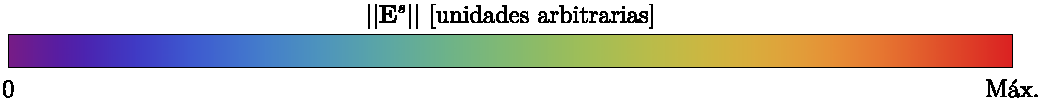
\includegraphics[scale=.85]{1-Teoria/figs/EsNorm.pdf}\\
%		\hspace{-4em}
%		\begin{subfigure}{.05\linewidth}\vspace{-3.25cm}\label{figs:ElectricMultipoles} \caption{ } \end{subfigure}
%		\hspace{-3em}
%		\begin{subfigure}{.9\linewidth}
%		\animategraphics[loop, autoplay,scale=.25]{10}{1-Teoria/figs/Ne11/Ne11_crop-}{0}{62}%
%		\animategraphics[loop, autoplay,scale=.25]{10}{1-Teoria/figs/Ne12/Ne12_crop-}{0}{62}%
%		\animategraphics[loop, autoplay,scale=.25]{10}{1-Teoria/figs/Ne13/Ne13_crop-}{0}{62}%
%		\animategraphics[loop, autoplay,scale=.25]{10}{1-Teoria/figs/Ne14/Ne14_crop-}{0}{62}
%		\end{subfigure}\\
%		\hspace{-4em}	
%		\begin{subfigure}{.05\linewidth}\vspace{-3.25cm}\label{figs:MagneticMultipoles} \caption{ } \end{subfigure}
%		\hspace{-3em}
%		\begin{subfigure}{.9\linewidth}			
%		\animategraphics[loop, autoplay,scale=.25]{10}{1-Teoria/figs/Mo11/Mo11_crop-}{0}{62}%
%		\animategraphics[loop, autoplay,scale=.25]{10}{1-Teoria/figs/Mo12/Mo12_crop-}{0}{62}%
%		\animategraphics[loop, autoplay,scale=.25]{10}{1-Teoria/figs/Mo13/Mo13_crop-}{0}{62}%
%		\animategraphics[loop, autoplay,scale=.25]{10}{1-Teoria/figs/Mo14/Mo14_crop-}{0}{62}%
%		\end{subfigure}
%		\caption{Contribuciones multipolares \textbf{a)} eléctricas $a_\ell$ y \textbf{b)} magnéticas $b_\ell$ de orden $\ell = 1,2,3$ y $4$ del campo esparcido $\vb{E}^s$ por una partícula esférica, evaluadas en una superficie matemática esférica y concéntrica a la partícula que radía los campos EMs, en donde el plano de la página corresponde al plano de oscilación del campo eléctrico incidente $\vb{E}^i$. En las gráficas presentadas, el color rojo corresponde a los valores máximos del campo eléctrico, mientras que los azules son los puntos menos intensos, donde se presentan los nodos en la superficie esférica.}
%		\label{fig:Multipolos}
%	\end{figure}
%	\begin{figure}[h!]\centering
%		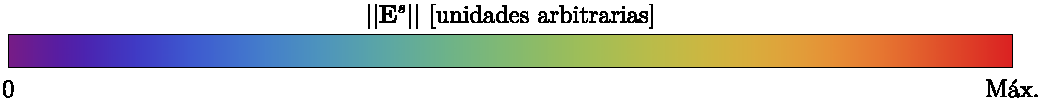
\includegraphics[scale=.85]{1-Teoria/figs/EsNorm.pdf}\\
%		\hspace{-4em}
%		\begin{subfigure}{.05\linewidth}\vspace{-3.25cm}\label{figs:ElectricMultipoles} \caption{ } \end{subfigure}
%		\hspace{-3em}
%		\begin{subfigure}{.9\linewidth}
%			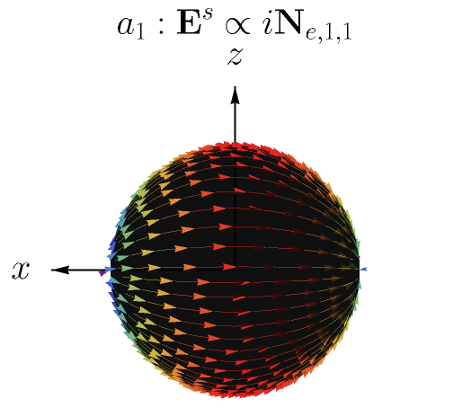
\includegraphics[scale=.25]{1-Teoria/figs/Ne11_static_crop.png}%
%			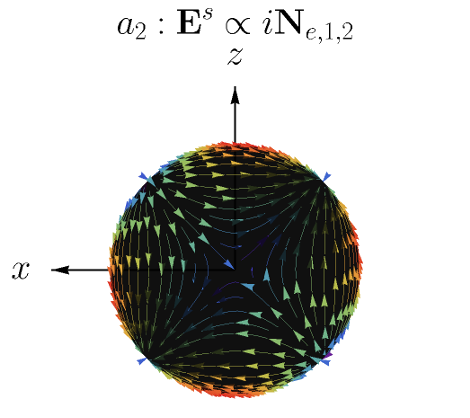
\includegraphics[scale=.25]{1-Teoria/figs/Ne12_static_crop.png}%
%			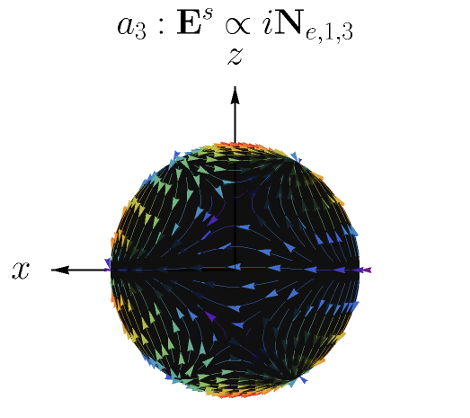
\includegraphics[scale=.25]{1-Teoria/figs/Ne13_static_crop.png}%
%			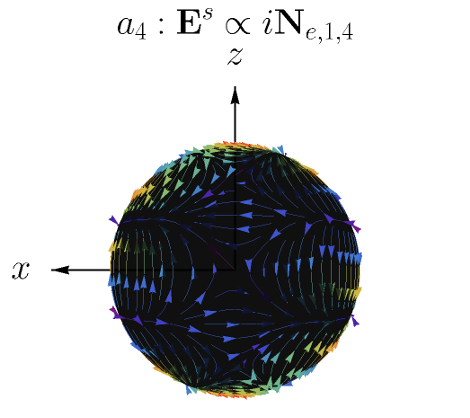
\includegraphics[scale=.25]{1-Teoria/figs/Ne14_static_crop.png}%
%		\end{subfigure}\\
%		\hspace{-4em}	
%		\begin{subfigure}{.05\linewidth}\vspace{-3.25cm}\label{figs:MagneticMultipoles} \caption{ } \end{subfigure}
%		\hspace{-3em}
%		\begin{subfigure}{.9\linewidth}			
%		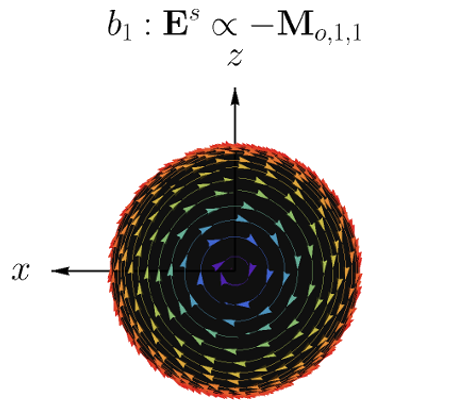
\includegraphics[scale=.25]{1-Teoria/figs/Mo11_static_crop.png}%
%		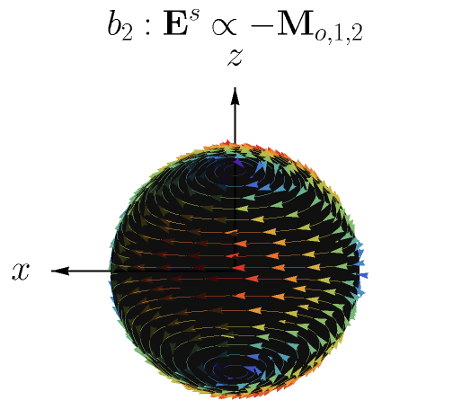
\includegraphics[scale=.25]{1-Teoria/figs/Mo12_static_crop.png}%
%		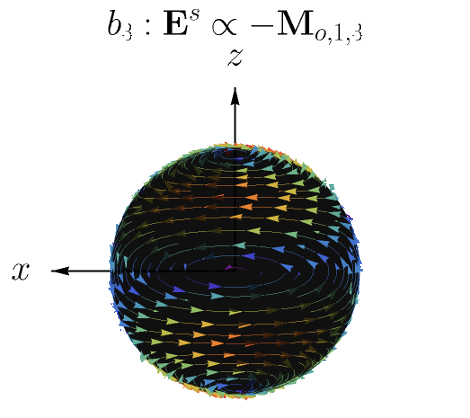
\includegraphics[scale=.25]{1-Teoria/figs/Mo13_static_crop.png}%
%		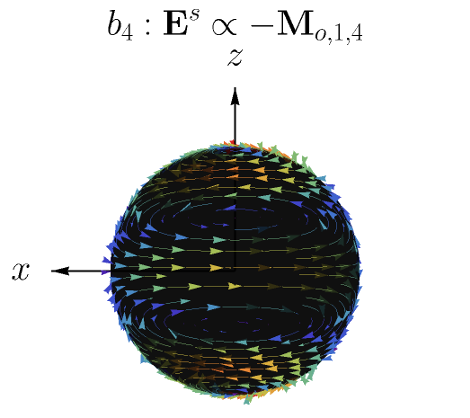
\includegraphics[scale=.25]{1-Teoria/figs/Mo14_static_crop.png}%
%		\end{subfigure}
%		\caption{Contribuciones multipolares \textbf{a)} eléctricas $a_\ell$ y \textbf{b)} magnéticas $b_\ell$ de orden $\ell = 1,2,3$ y $4$ del campo esparcido $\vb{E}^s$ por una partícula esférica, evaluadas en una superficie matemática esférica y concéntrica a la partícula que radia los campos EMs, en donde el plano de la página corresponde al plano de oscilación del campo eléctrico incidente $\vb{E}^i$. En las gráficas presentadas, el color rojo corresponde a los valores máximos del campo eléctrico, mientras que los azules son los puntos menos intensos, donde se presentan los nodos ($\vb{E}^s\approx \vb{0}$) en la superficie esférica.}
%		\label{fig:Multipolos}
%	\end{figure}
	\begin{figure}[h!]\centering
		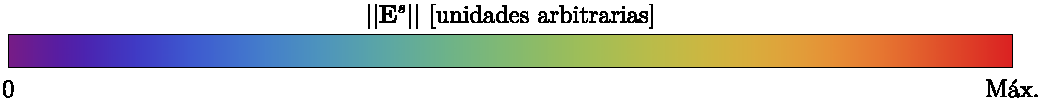
\includegraphics[scale=.85]{1-Teoria/figs/EsNorm.pdf}\\
		\hspace{-3em}
		\begin{subfigure}{.05\linewidth}\vspace{-3.25cm}\label{figs:ElectricMultipoles} \caption{ } \end{subfigure}
		\hspace{-3em}
		\begin{subfigure}{.9\linewidth}
			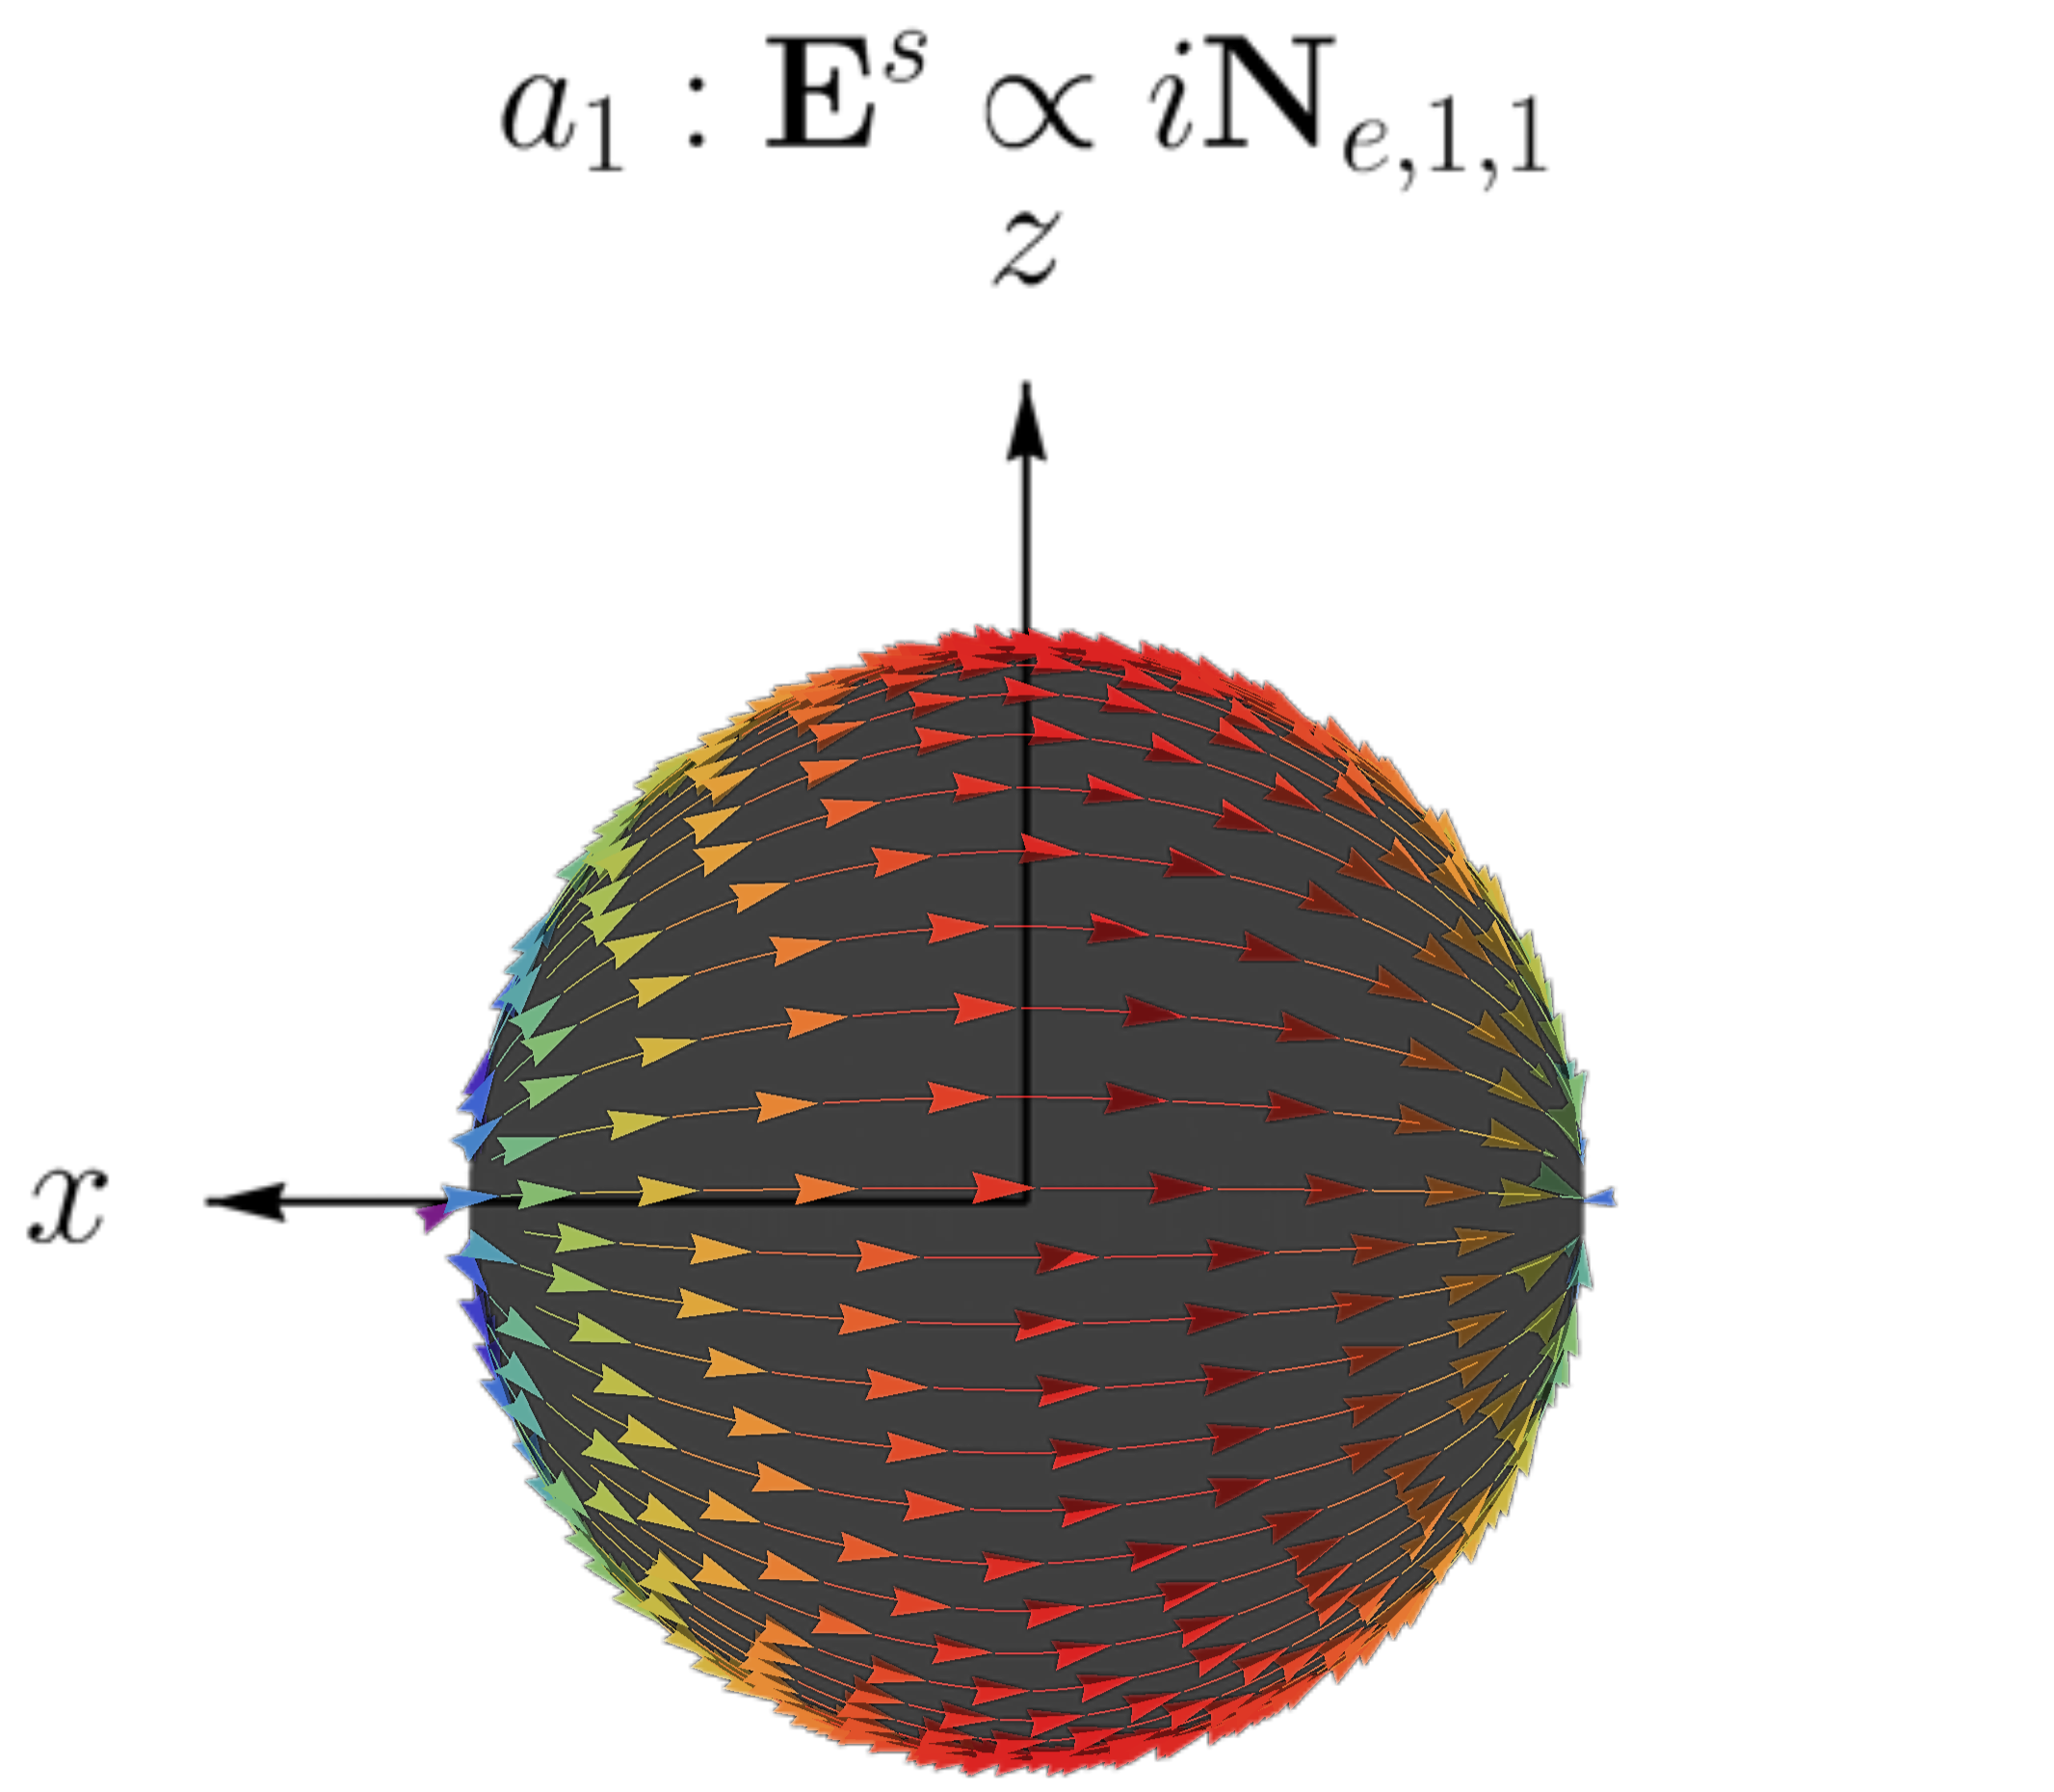
\includegraphics[scale=.25, trim={00 00 80 00}, clip]{1-Teoria/figs/Ne11_static.png}%
			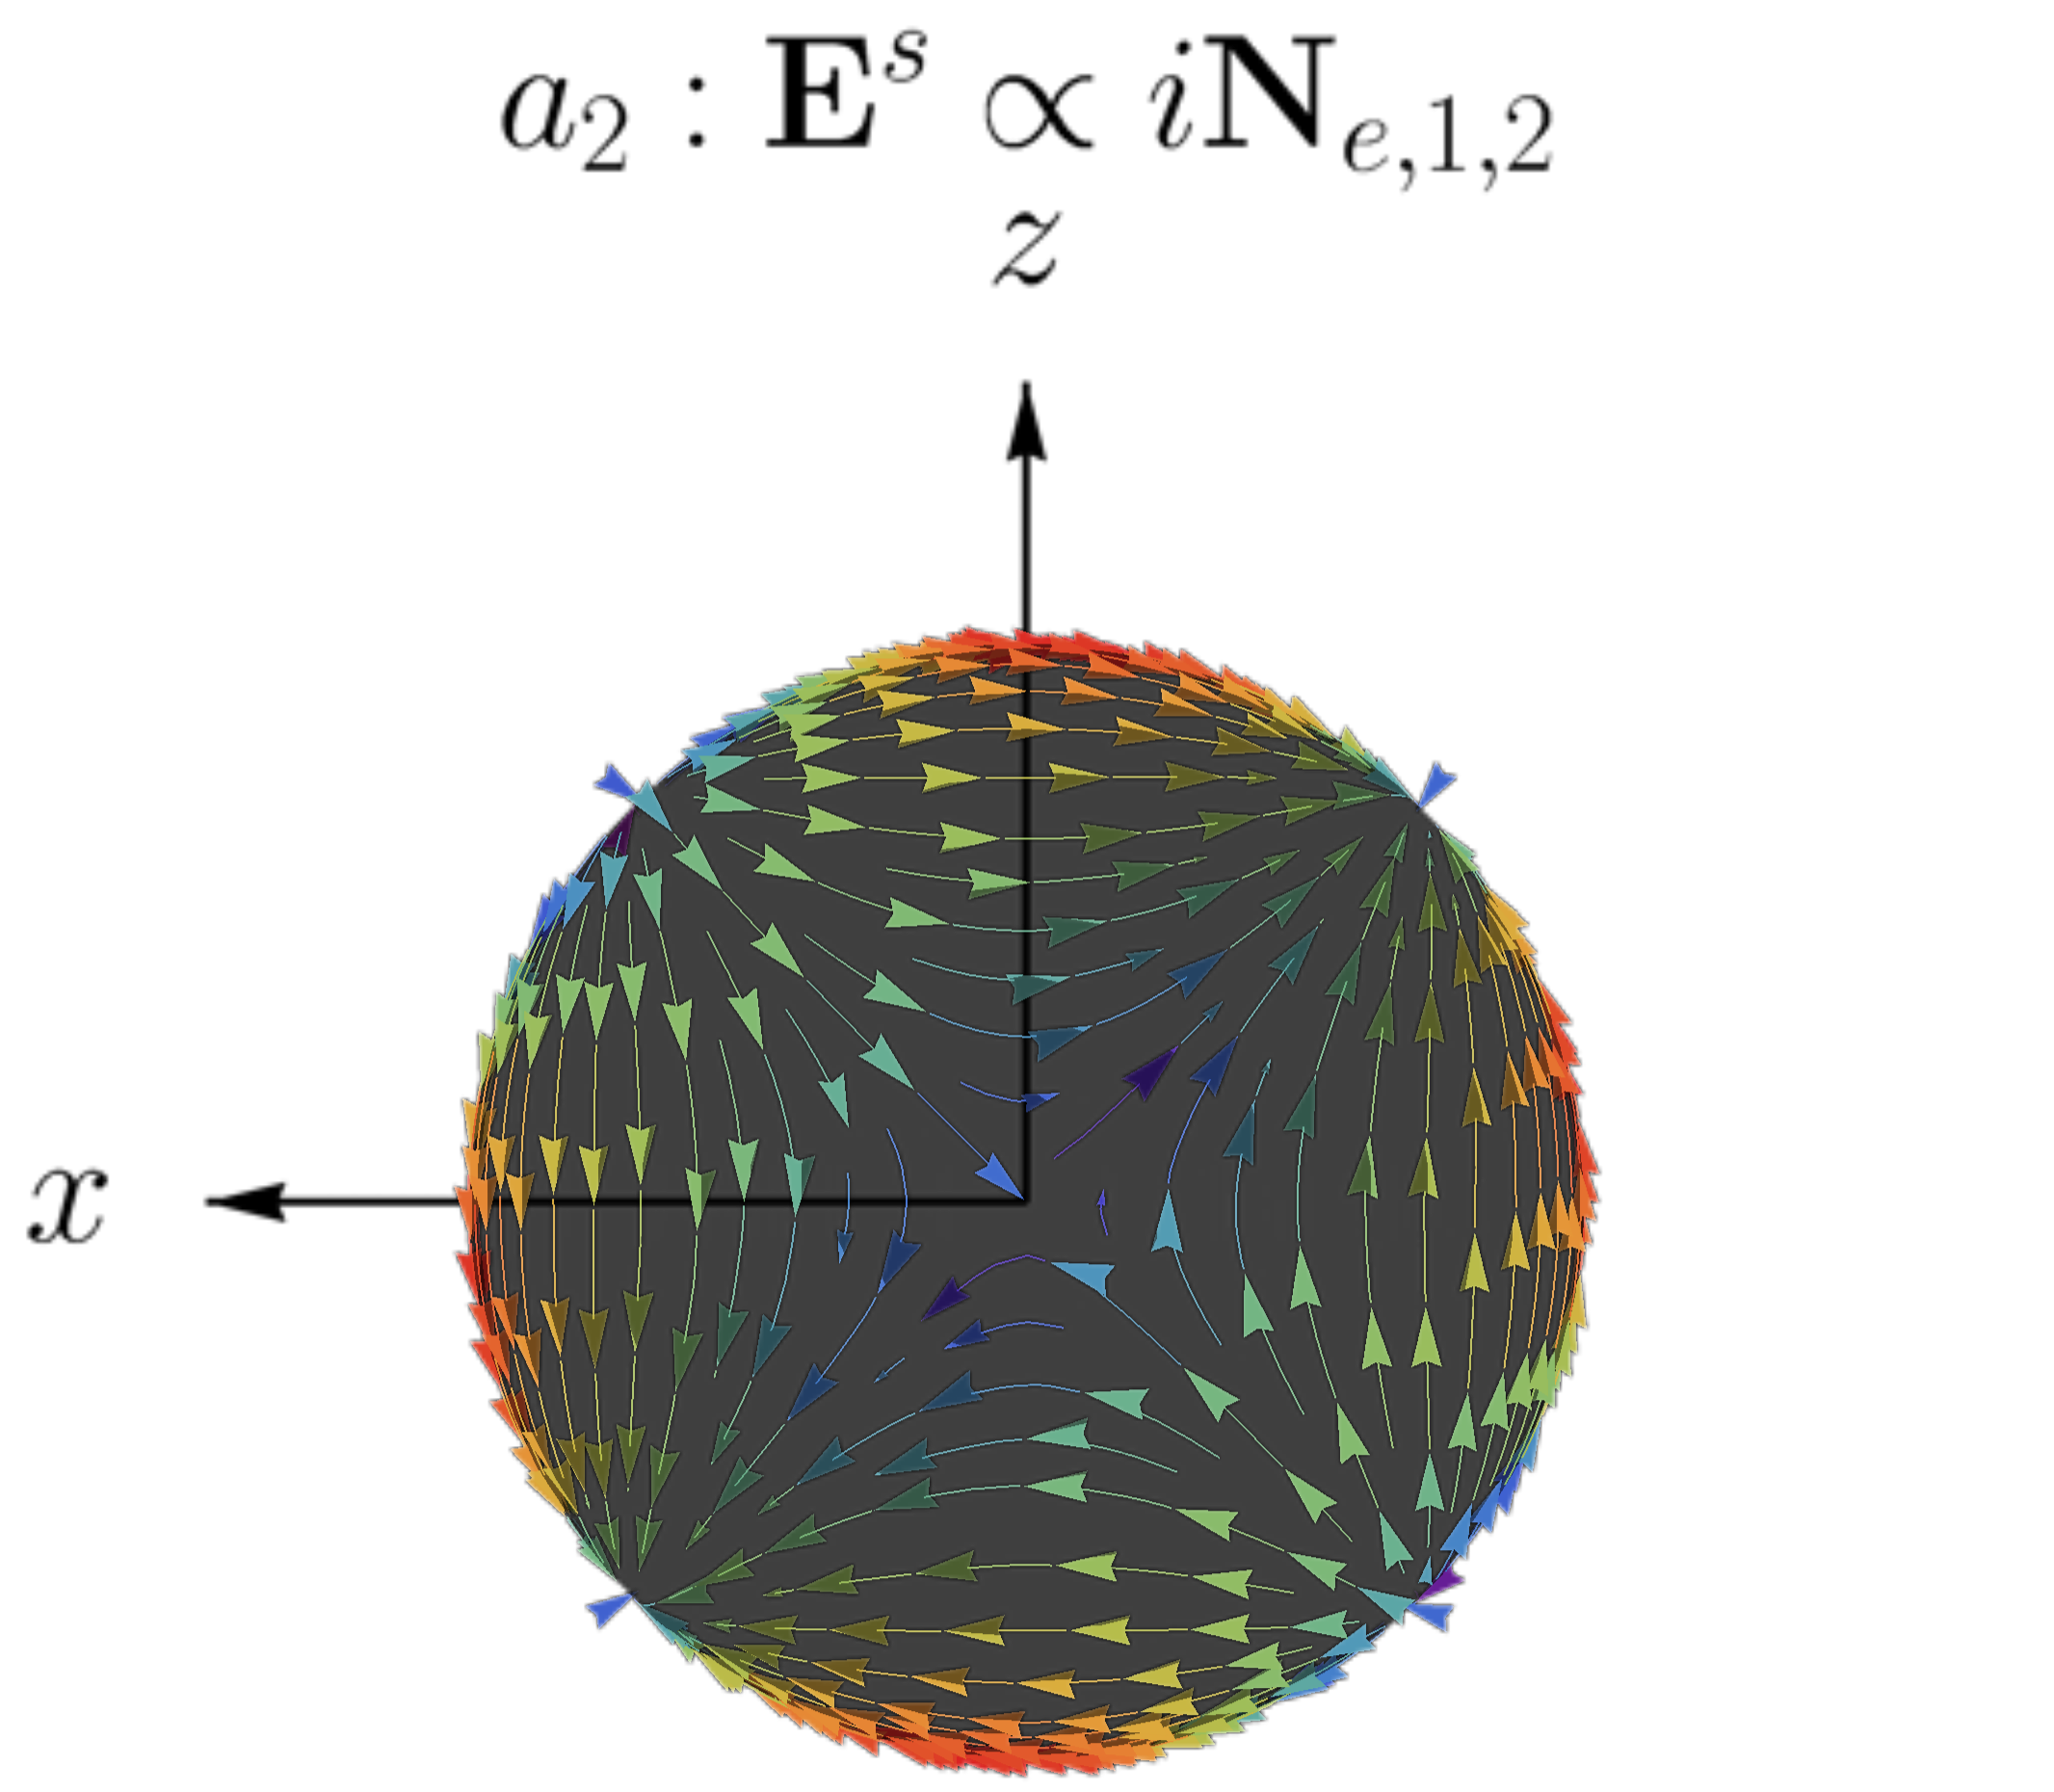
\includegraphics[scale=.25, trim={00 00 80 00}, clip]{1-Teoria/figs/Ne12_static.png}%
			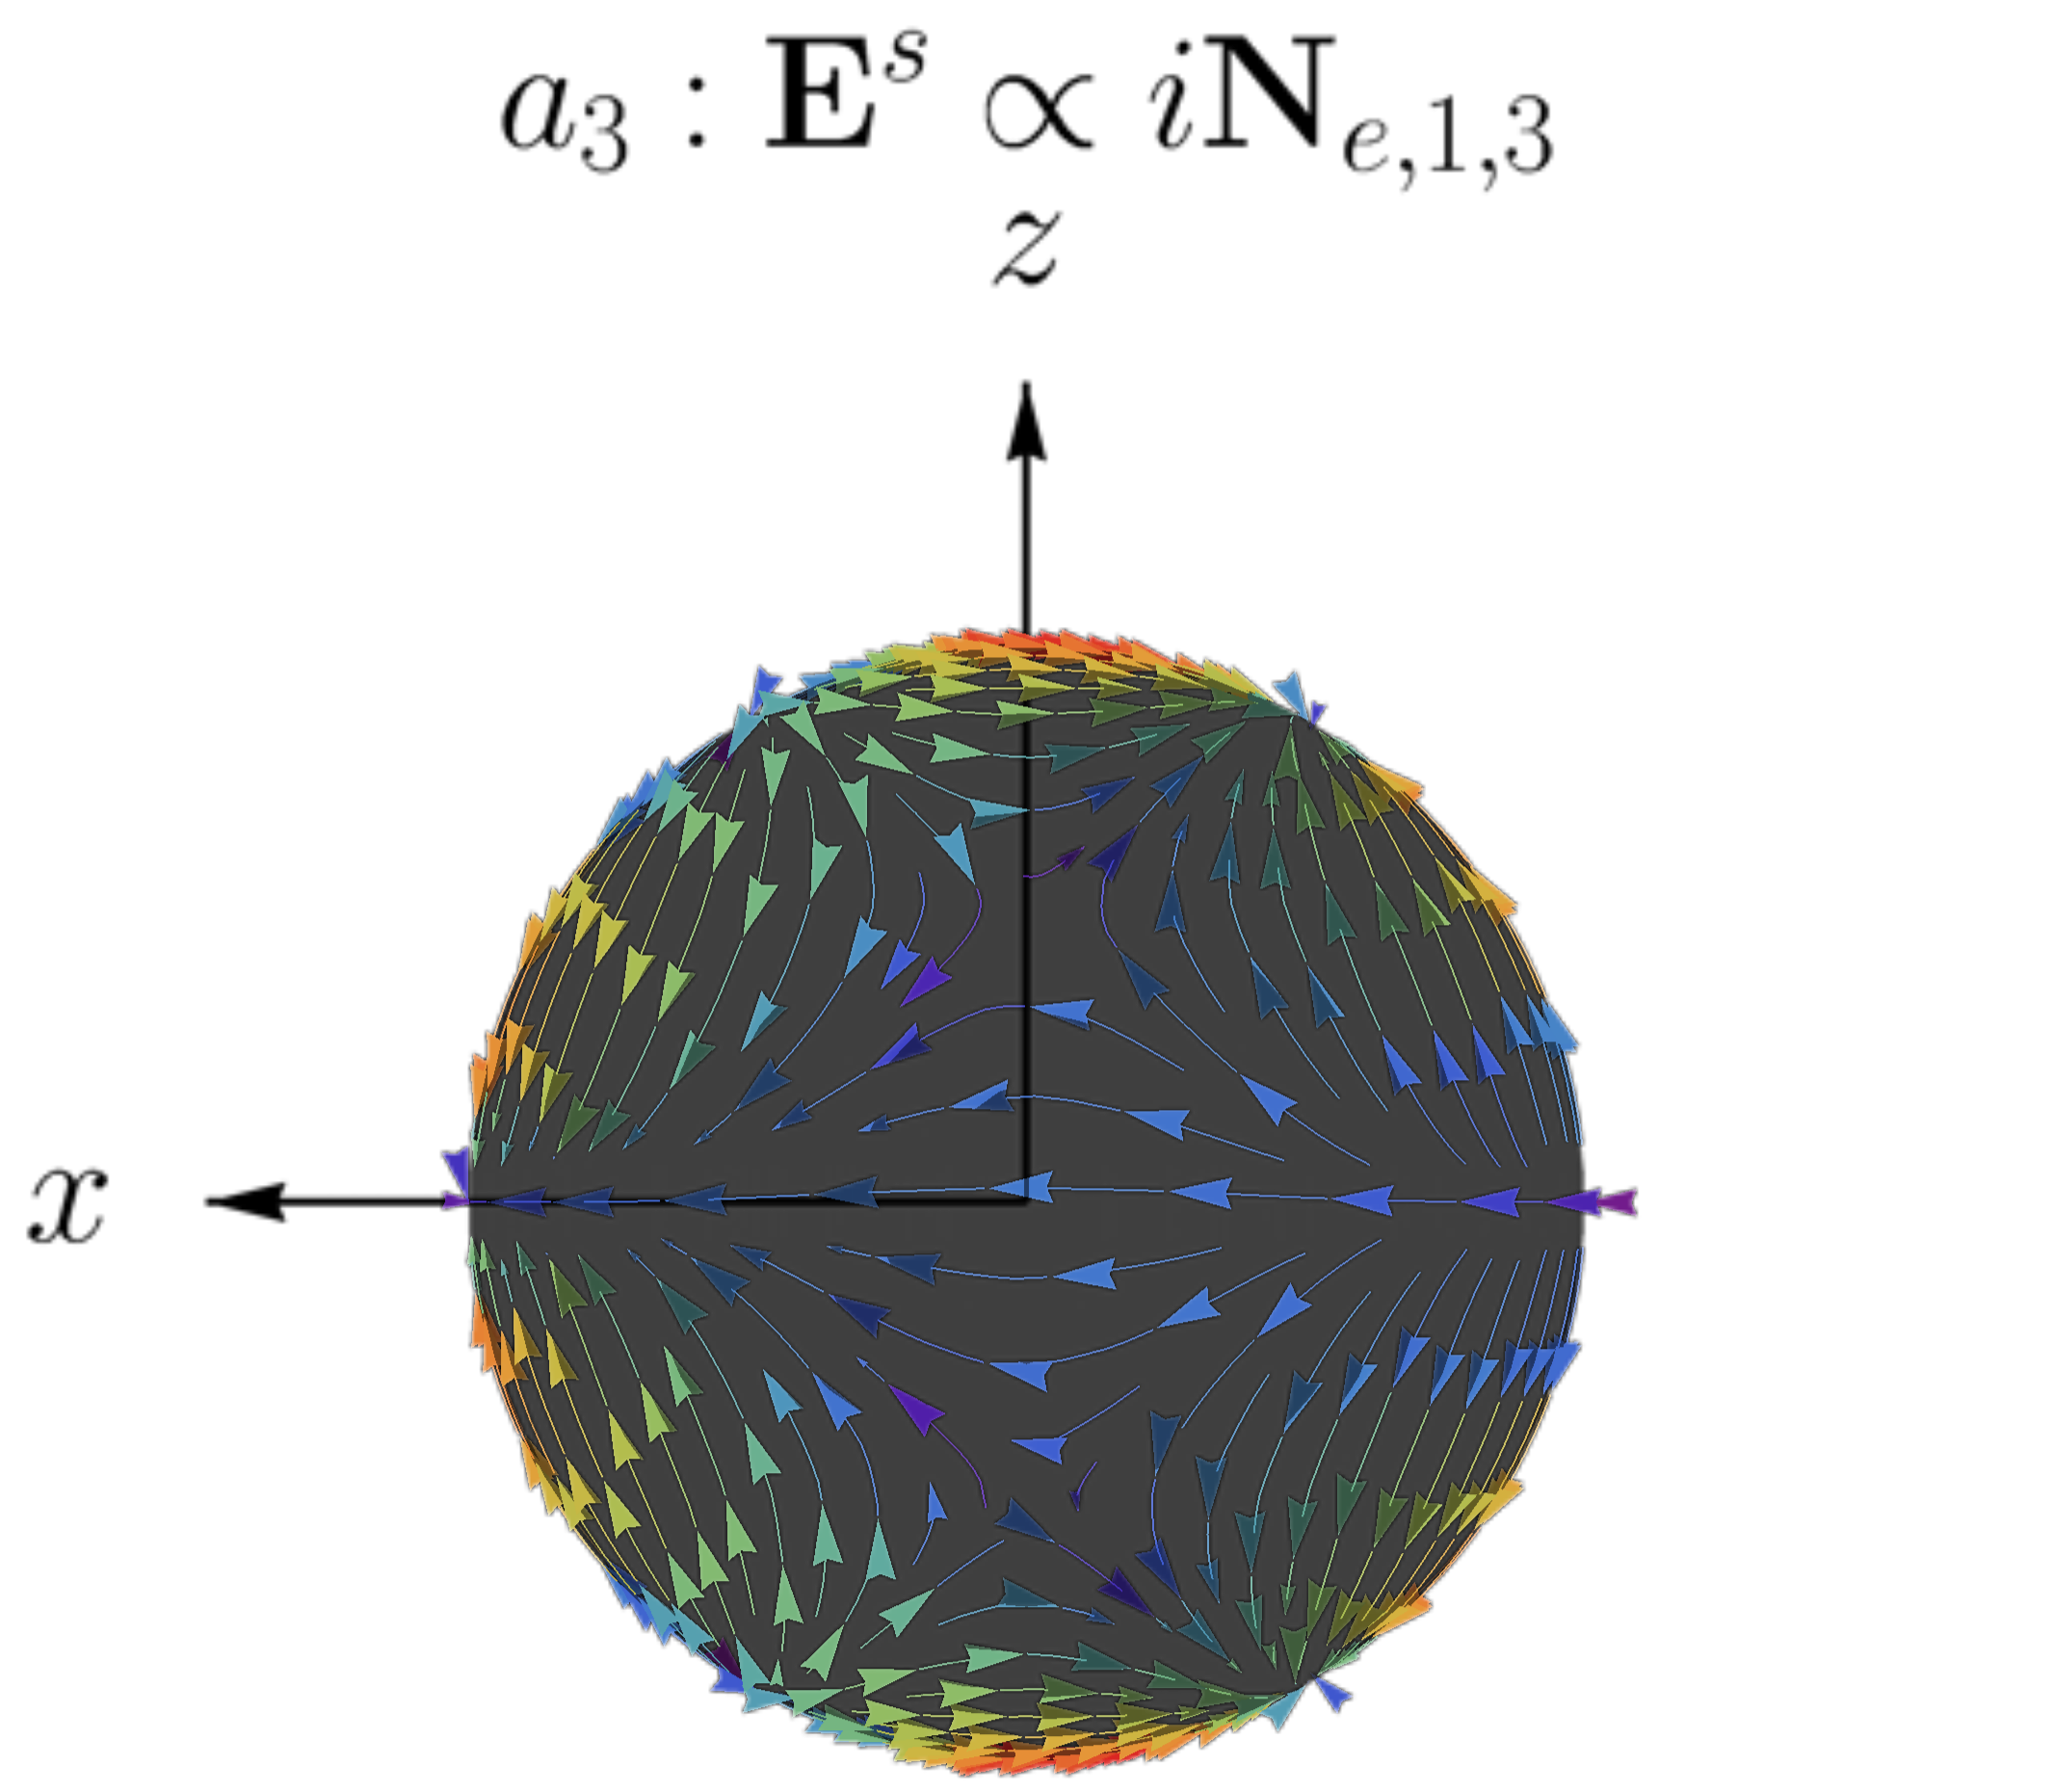
\includegraphics[scale=.25, trim={00 00 80 00}, clip]{1-Teoria/figs/Ne13_static.png}%
			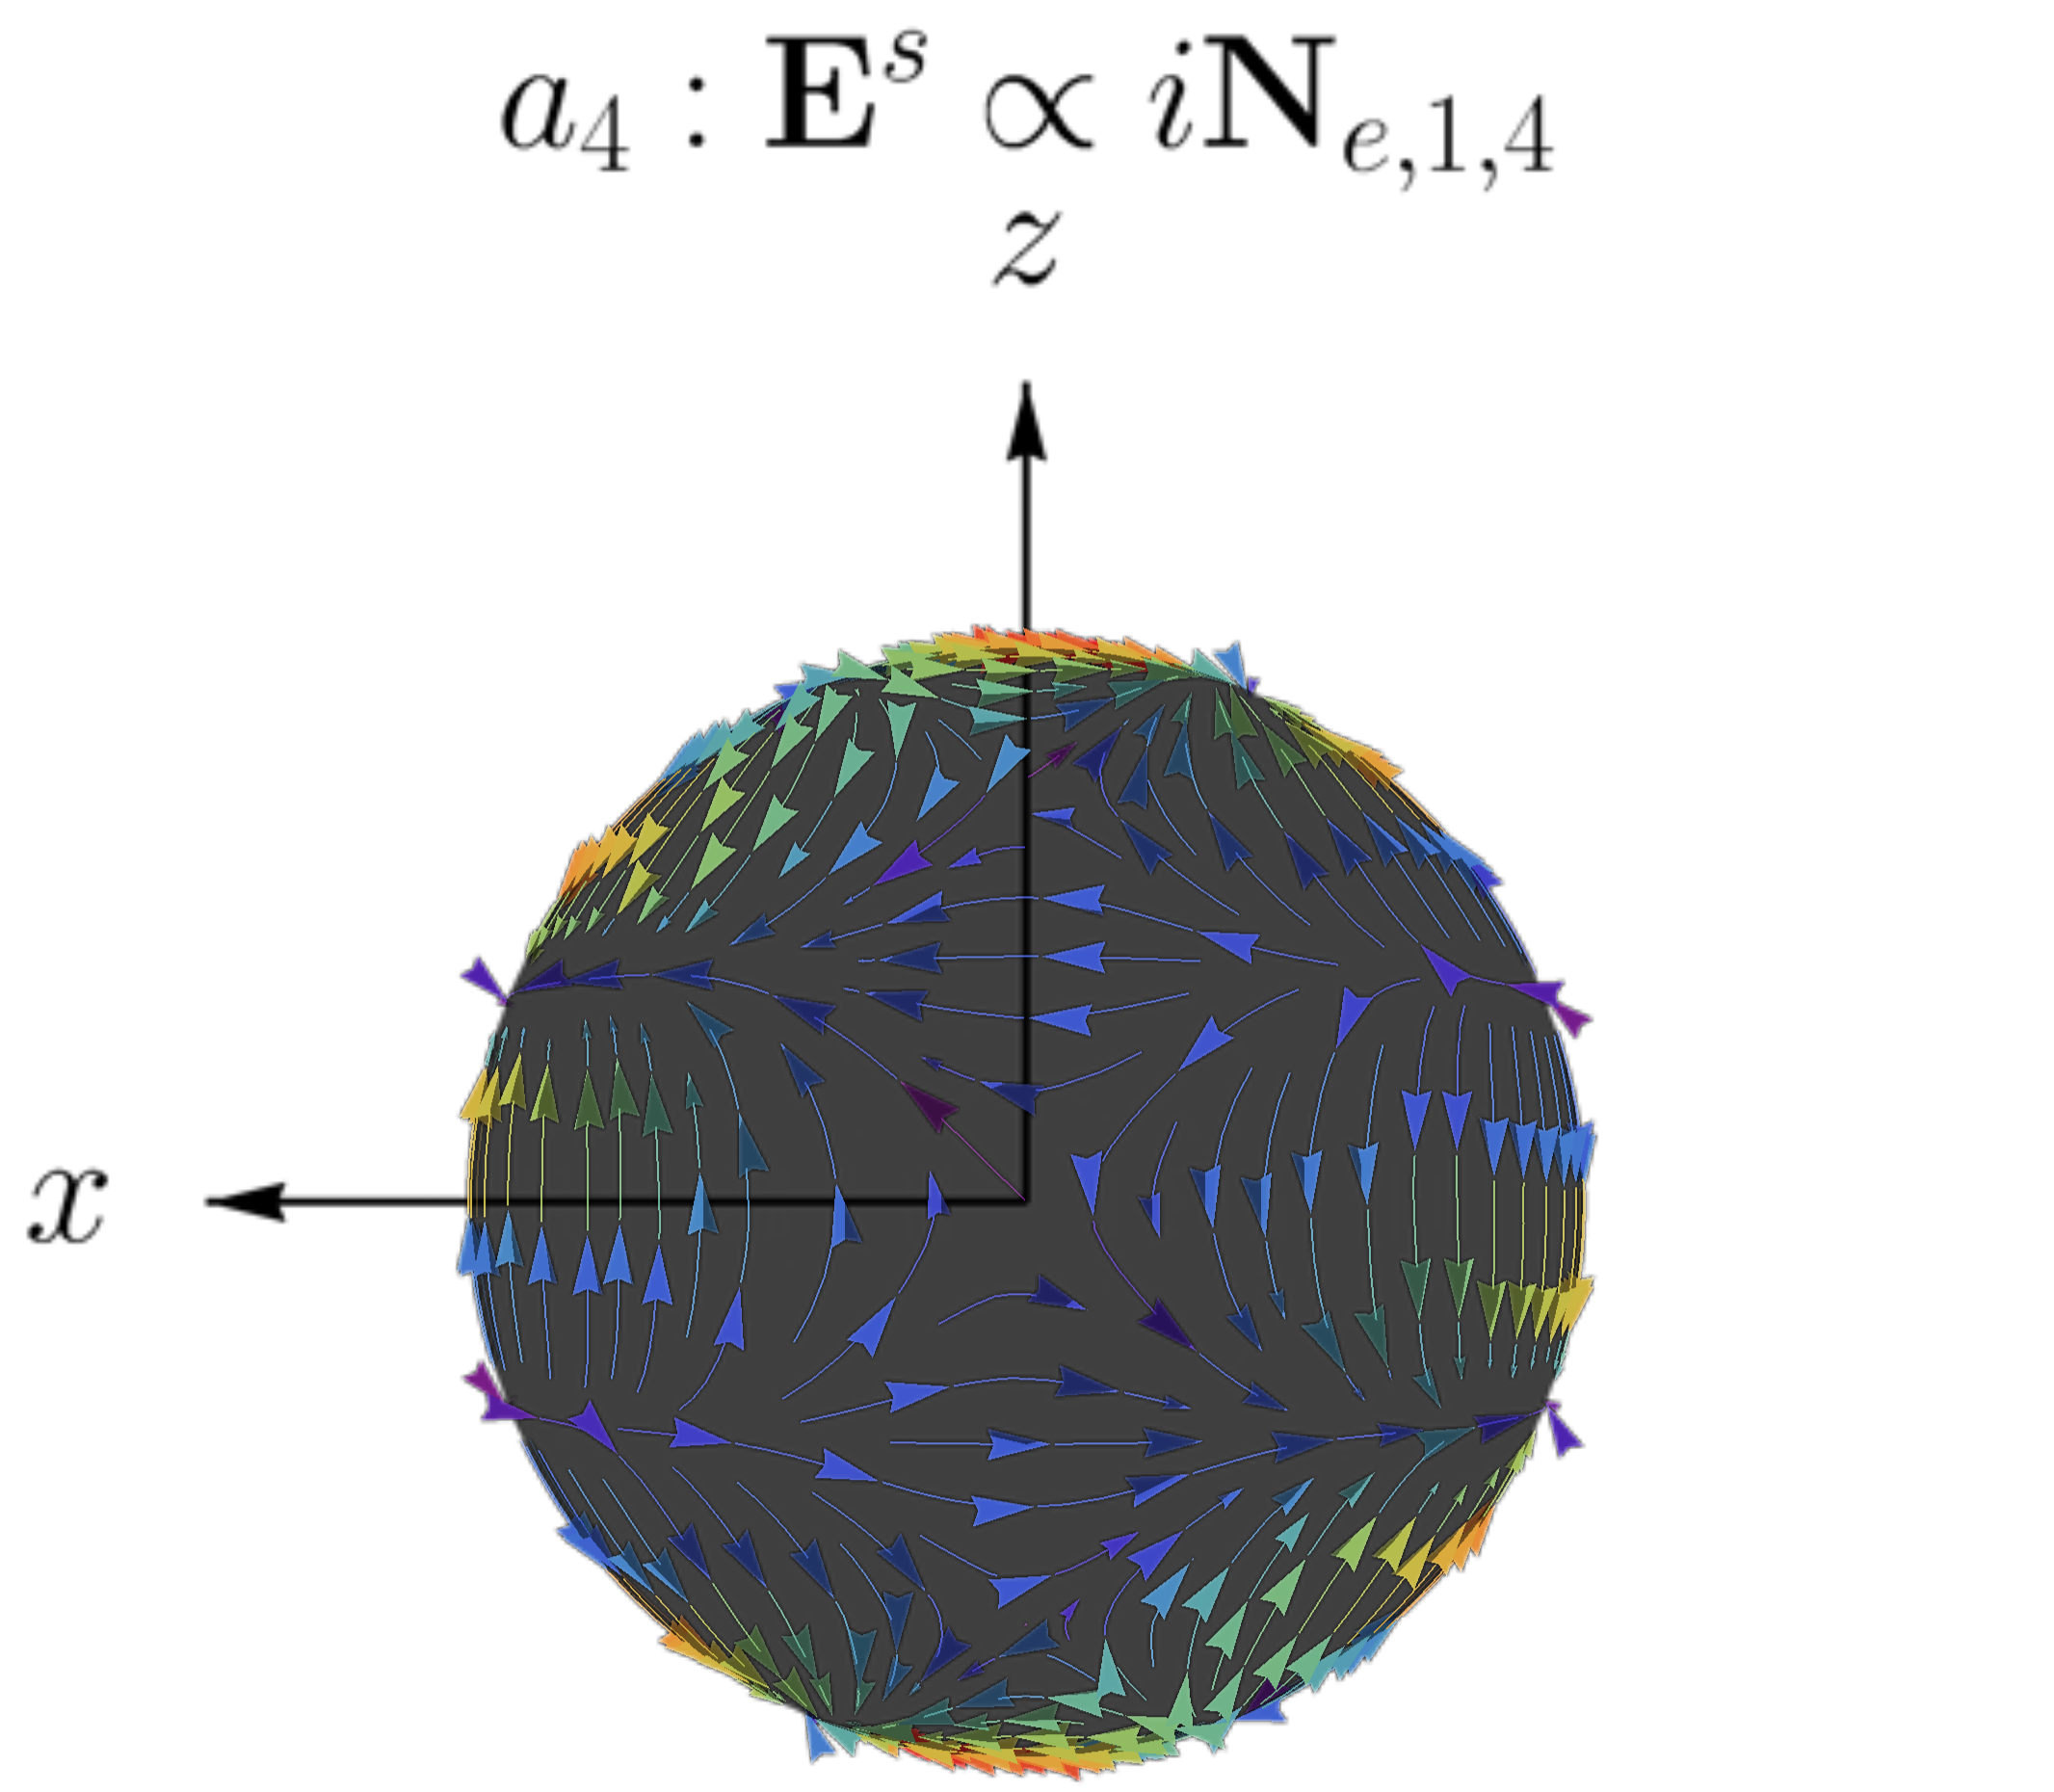
\includegraphics[scale=.25, trim={00 00 80 00}, clip]{1-Teoria/figs/Ne14_static.png}%
		\end{subfigure}\\
		\hspace{-3em}	
		\begin{subfigure}{.05\linewidth}\vspace{-3.25cm}\label{figs:MagneticMultipoles} \caption{ } \end{subfigure}
		\hspace{-3em}
		\begin{subfigure}{.9\linewidth}			
		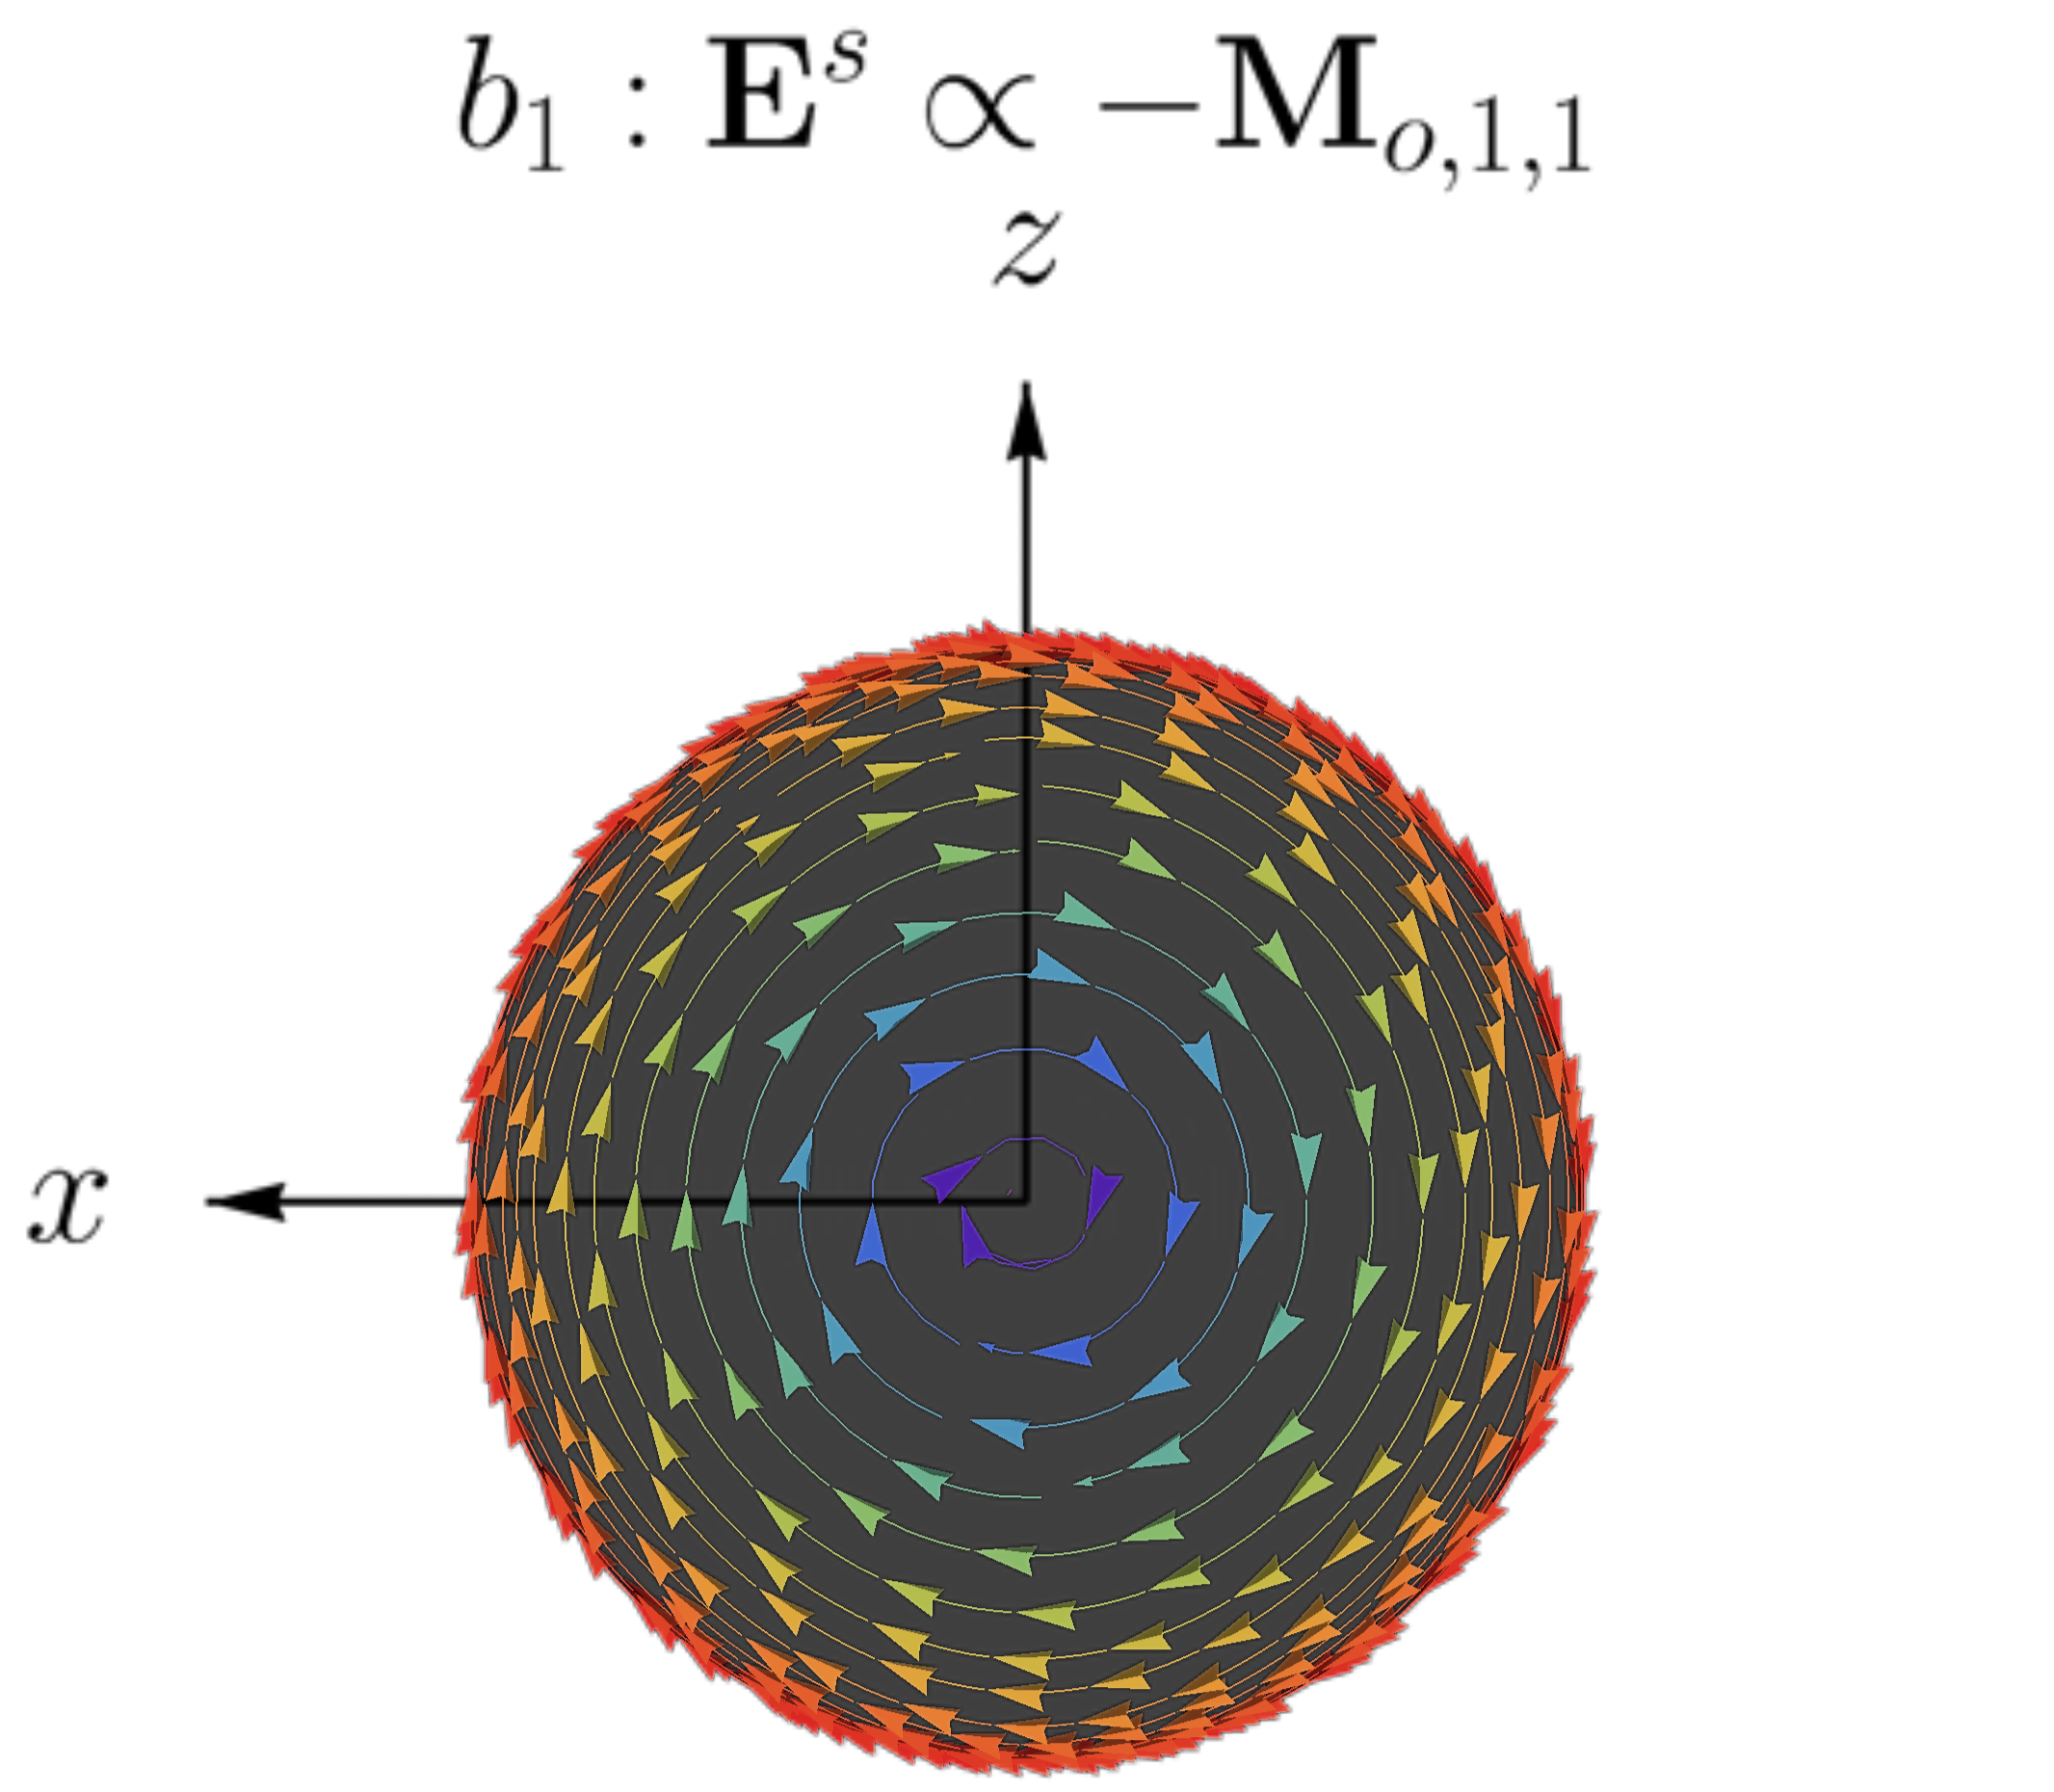
\includegraphics[scale=.25,trim={00 00 80 00}, clip]{1-Teoria/figs/Mo11_static.png}%
		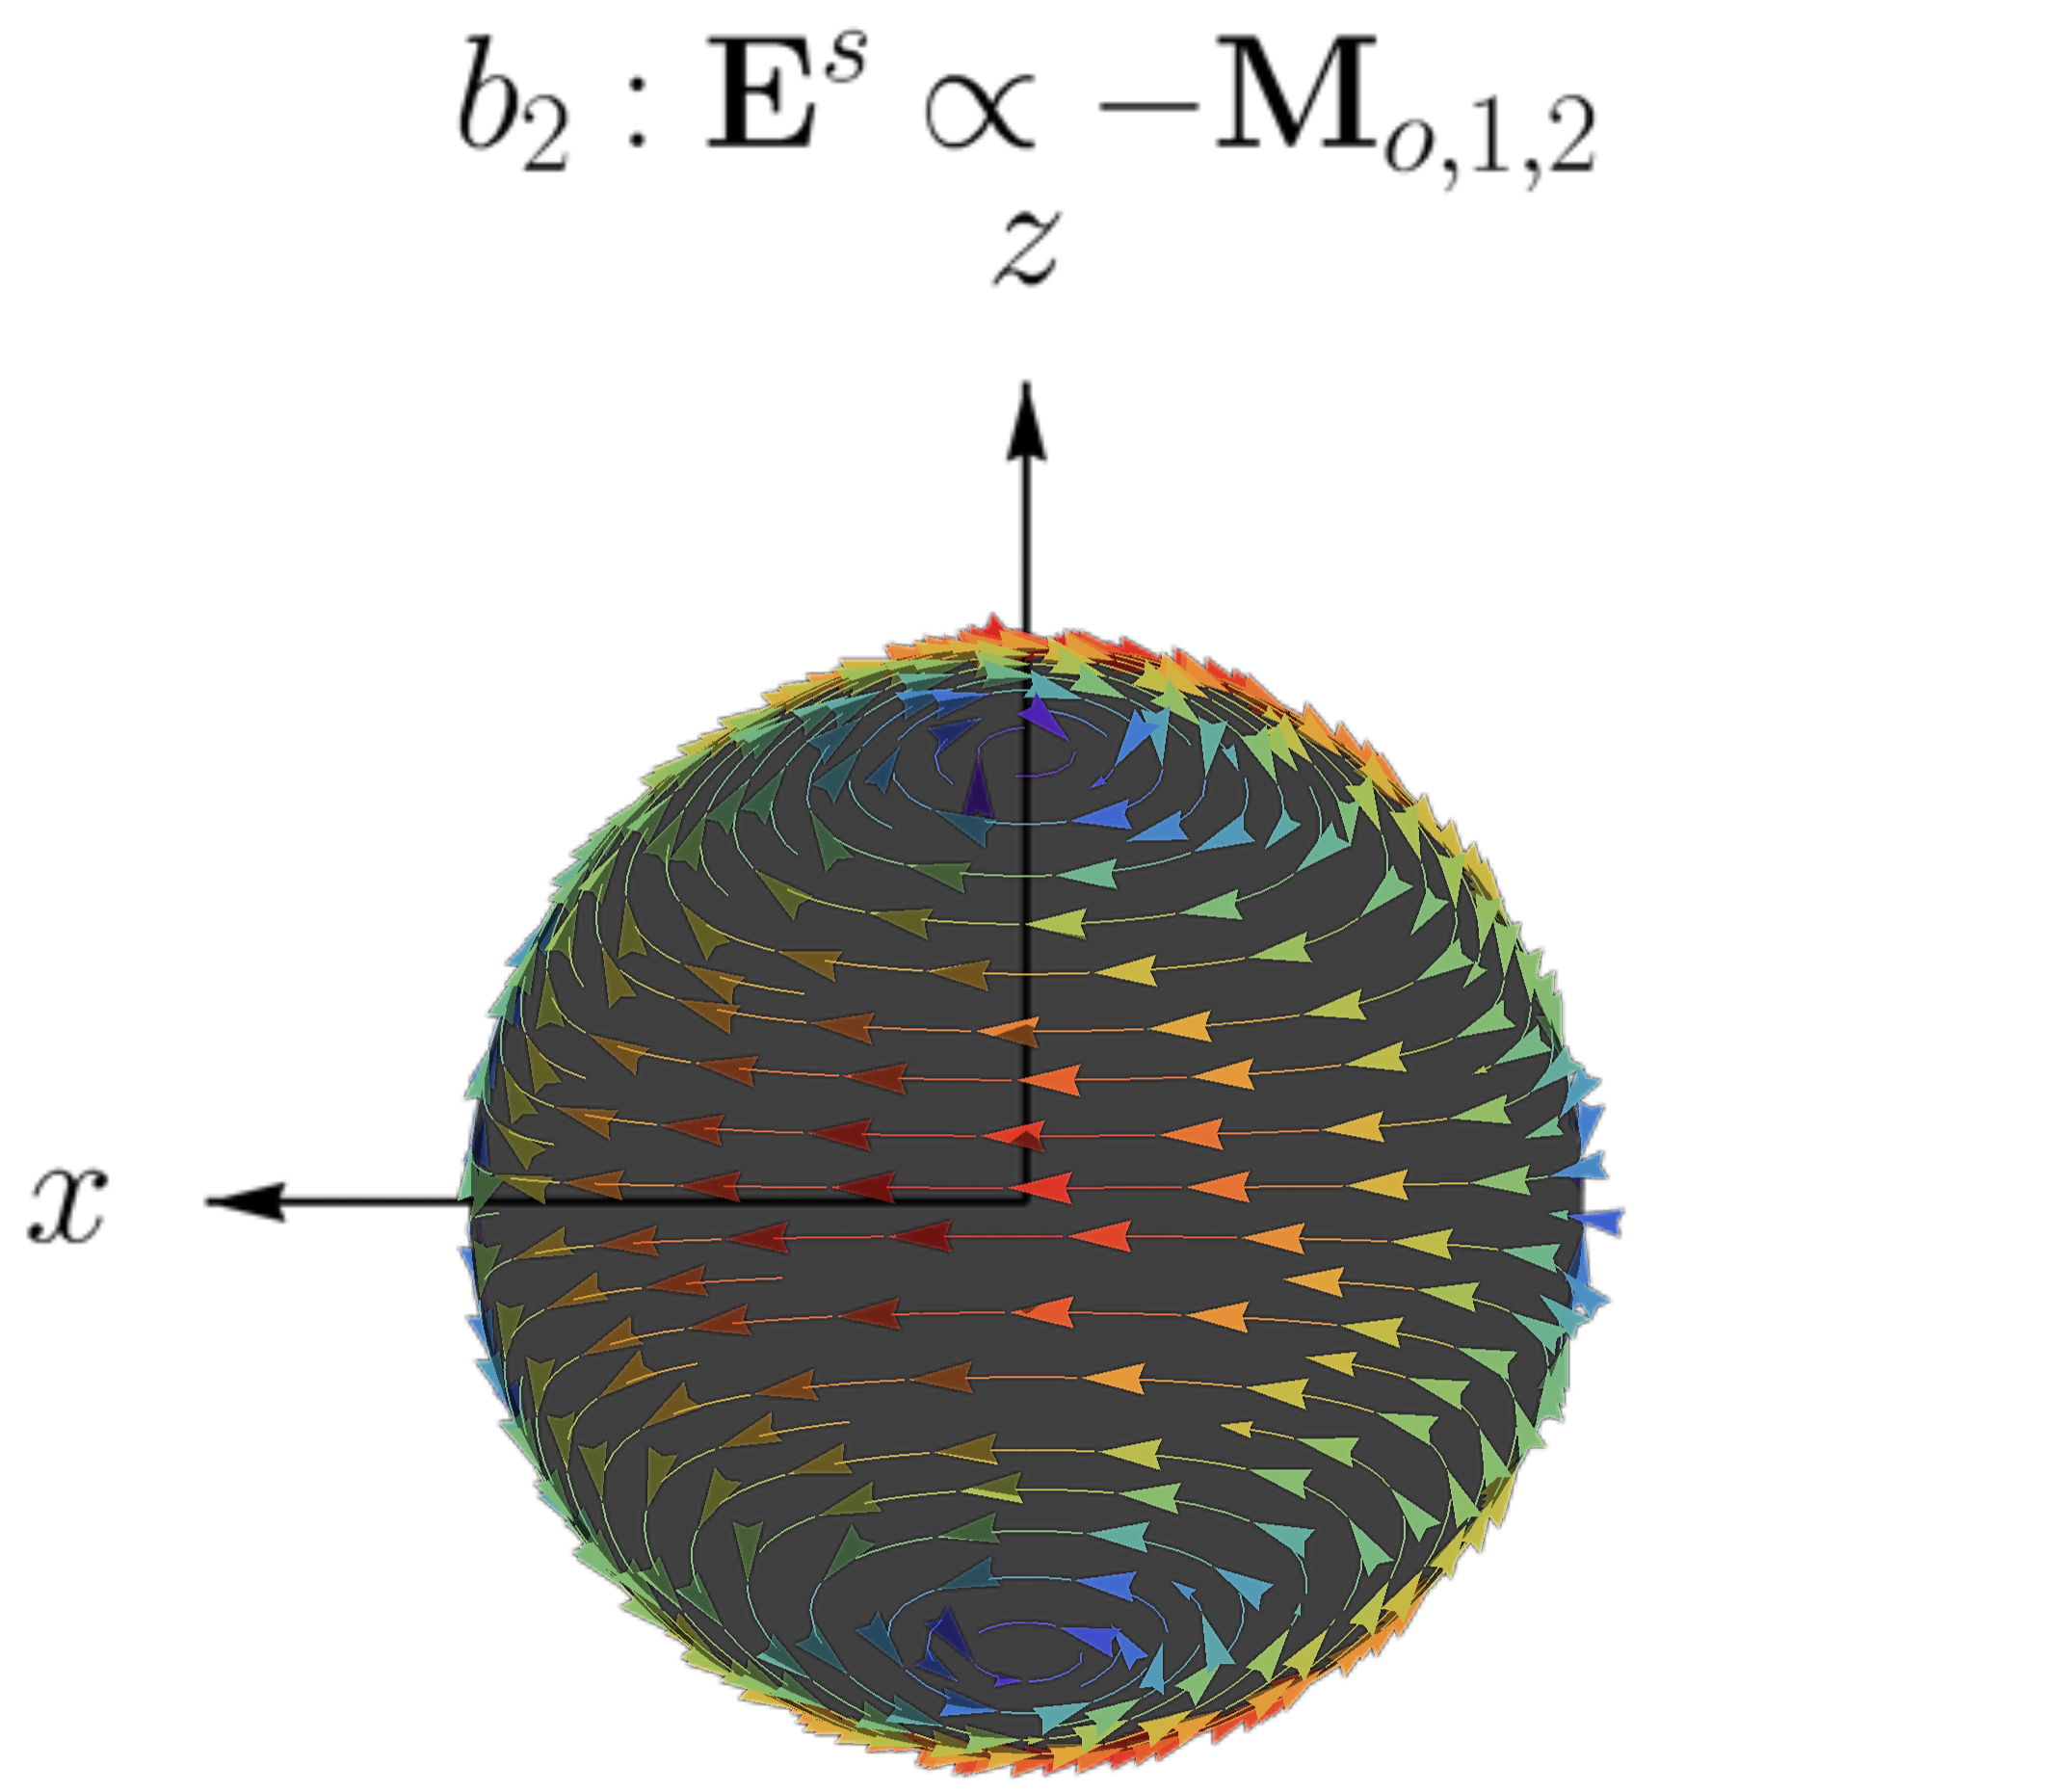
\includegraphics[scale=.25,trim={00 00 80 00}, clip]{1-Teoria/figs/Mo12_static.png}%
		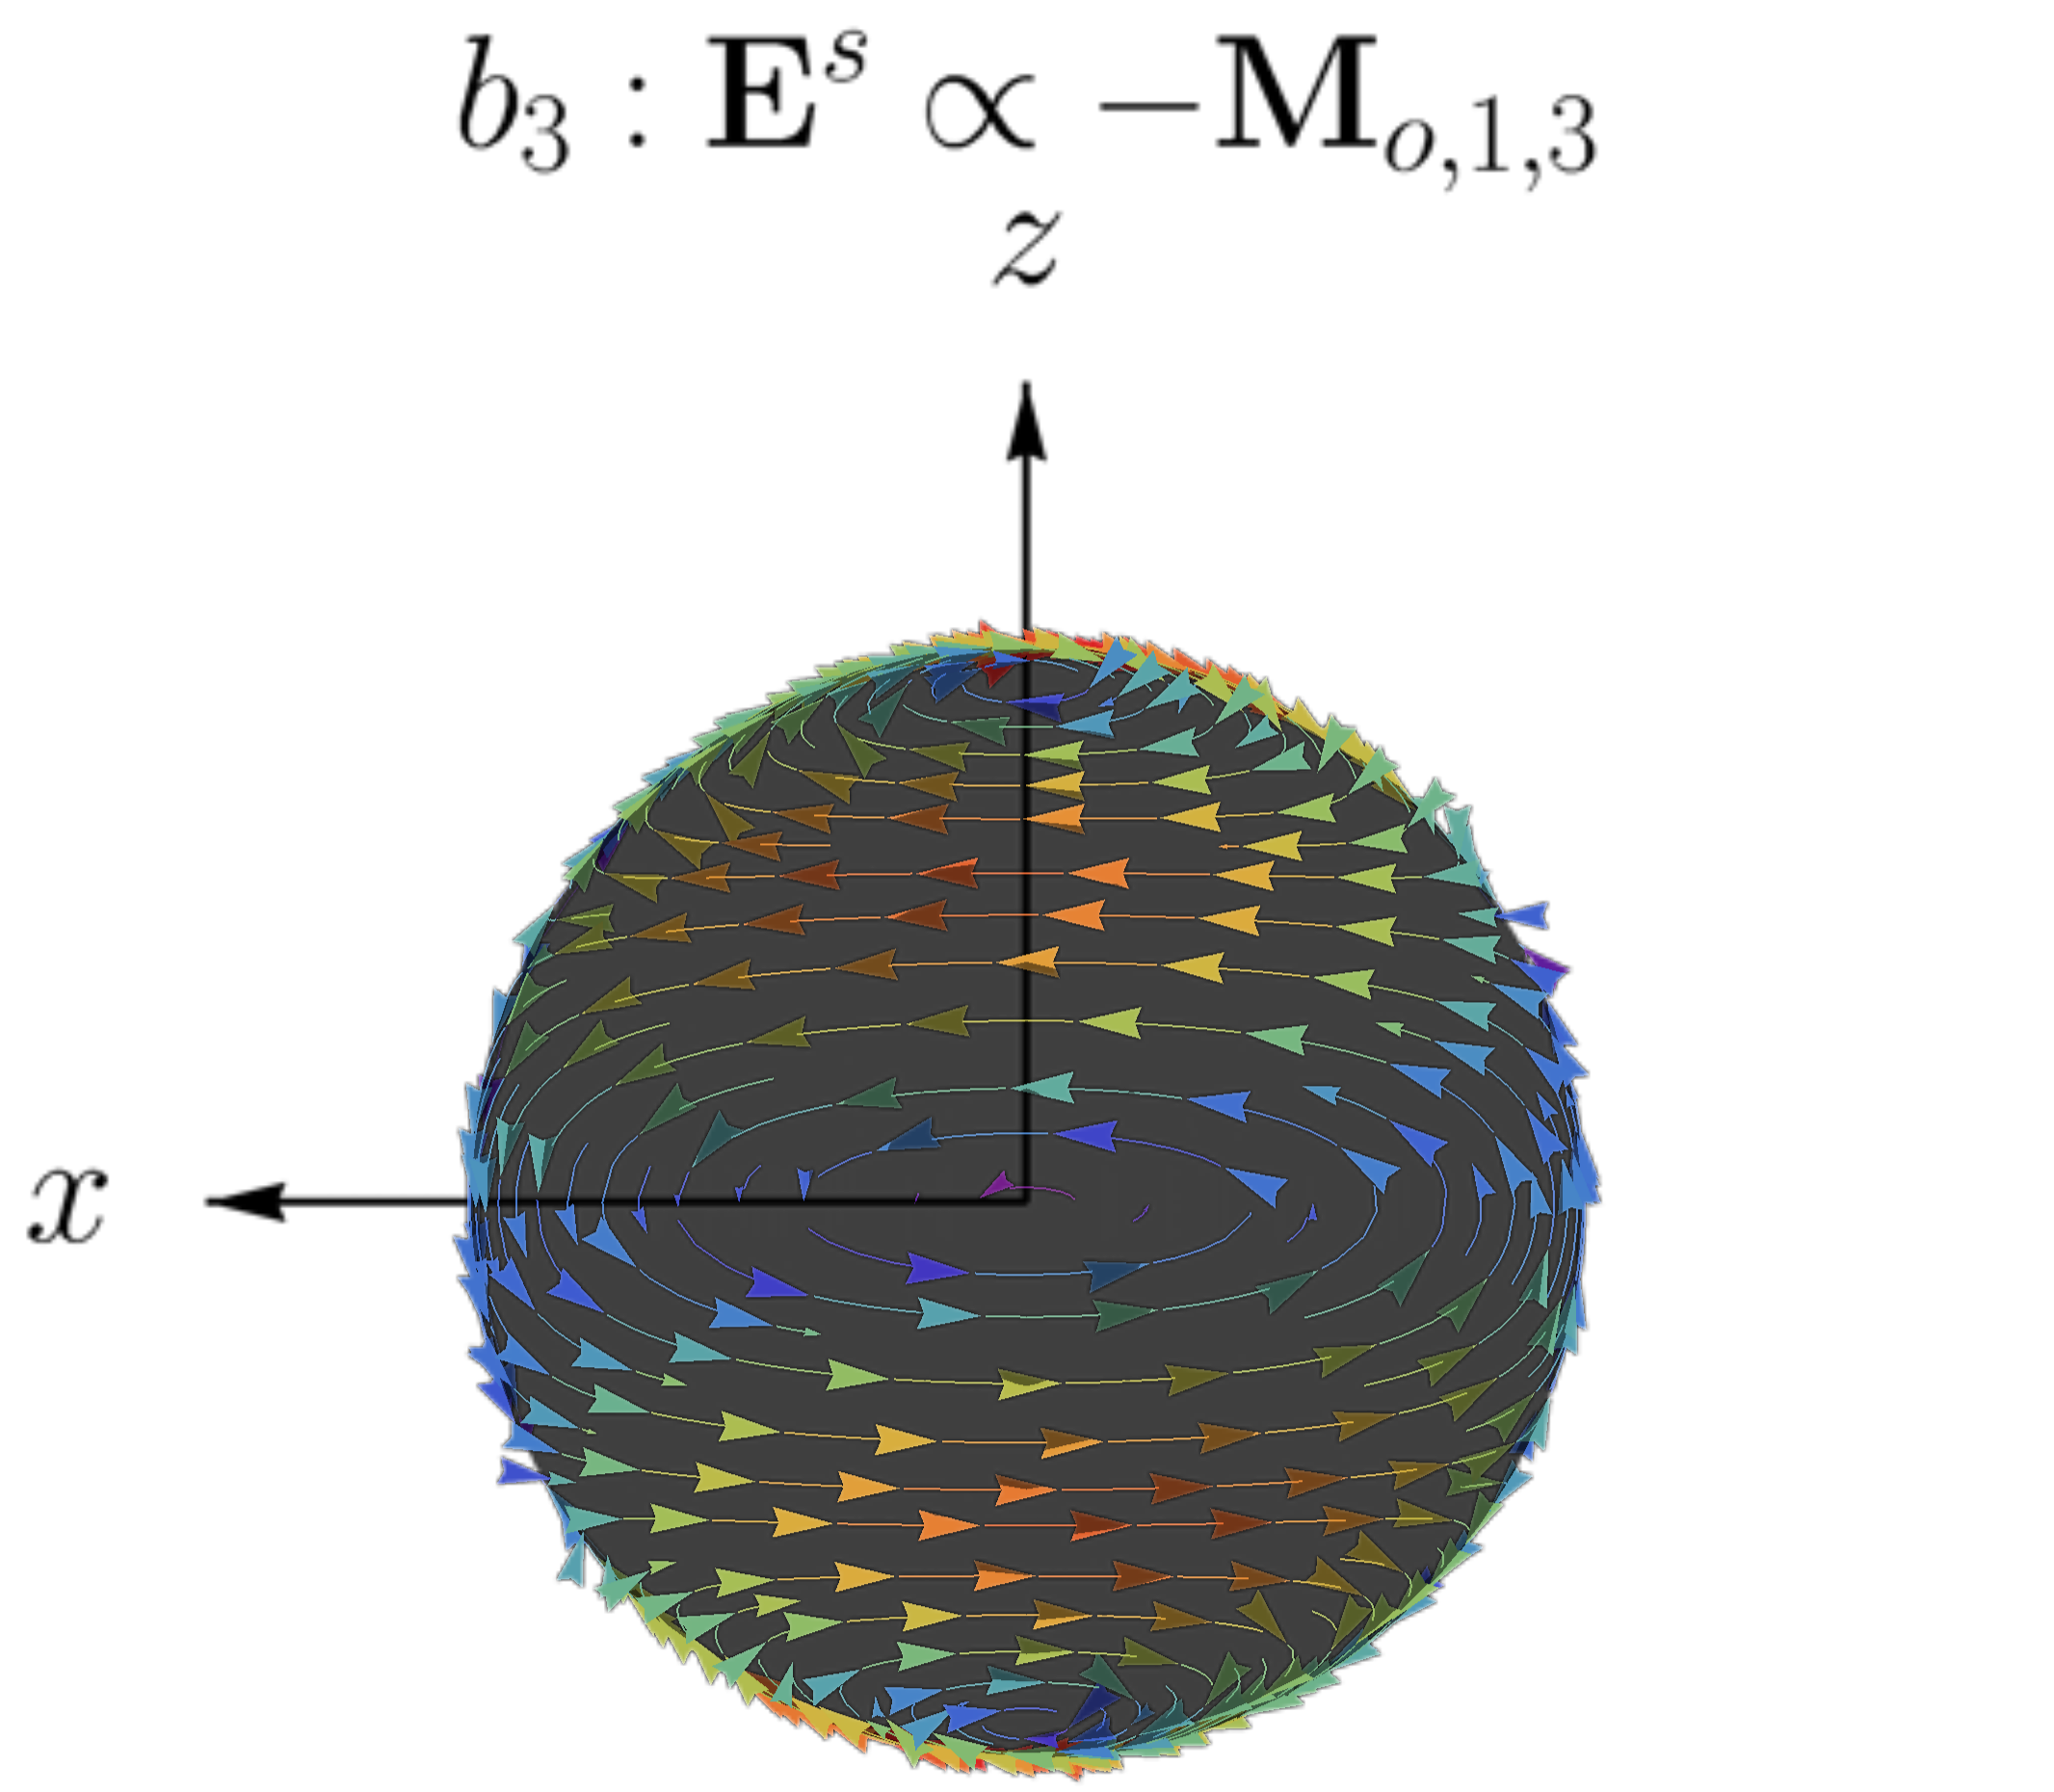
\includegraphics[scale=.25,trim={00 00 80 00}, clip]{1-Teoria/figs/Mo13_static.png}%
		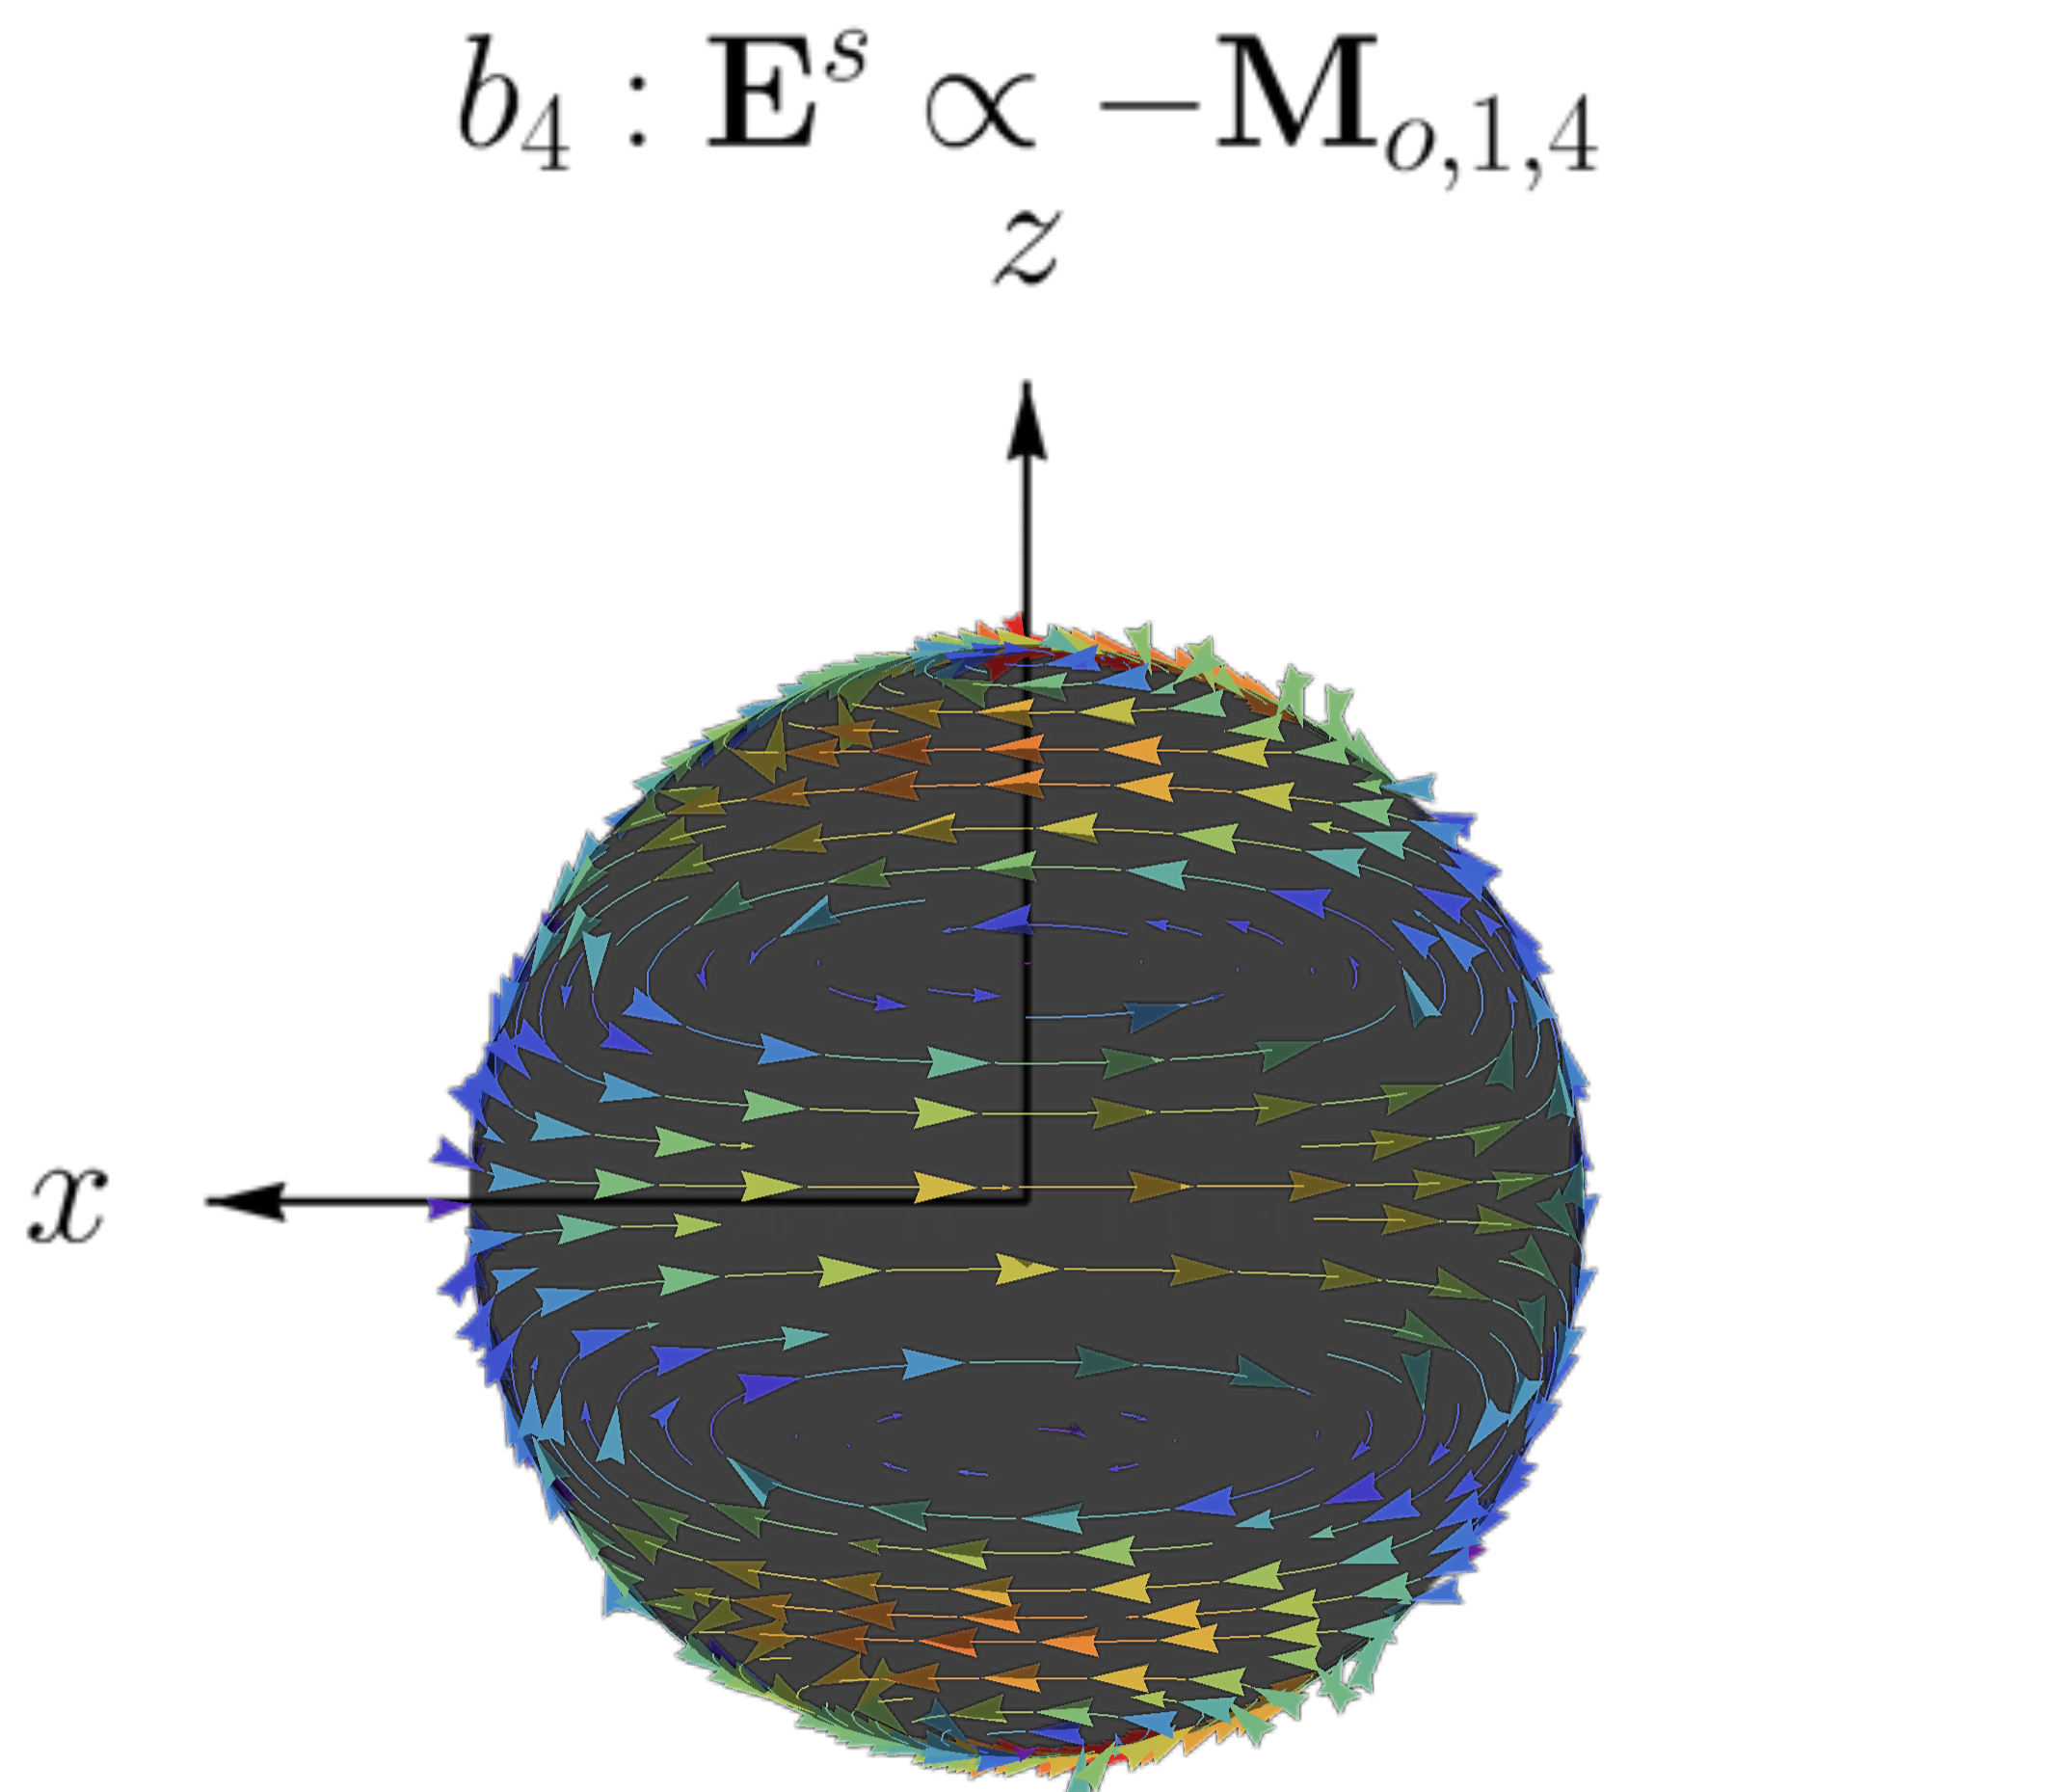
\includegraphics[scale=.25,trim={00 00 80 00}, clip]{1-Teoria/figs/Mo14_static.png}%
		\end{subfigure}
		\caption{Contribuciones multipolares \textbf{a)} eléctricas $a_\ell$ y \textbf{b)} magnéticas $b_\ell$ de orden $\ell = 1,2,3$ y $4$ del campo esparcido $\vb{E}^s$ por una partícula esférica, evaluadas en una superficie matemática esférica y concéntrica a la partícula que radia los campos EMs, en donde el plano de la página corresponde al plano de oscilación del campo eléctrico incidente $\vb{E}^i$. En las gráficas, el color rojo corresponde a los valores máximos del campo eléctrico, mientras que los azules son los puntos menos intensos, donde se presentan los nodos ($\vb{E}^s\approx \vb{0}$) en la superficie esférica.}
		\label{fig:Multipolos}
	\end{figure}

Los campos EMs esparcidos [Ecs. \eqref{eq:EHsAEV}] se calcularon al considerar una onda plana monocromática incidente $\vb{E}^i$ polarizada en la dirección $\vu{e}_x$. Sin embargo, debido a la simetría de la esfera, una onda plana polarizada en la dirección $\vu{e}_y$ se describe mediante la transformación $\varphi\to\varphi+\pi/2$, por lo que los campos EMs esparcidos y dentro de la esfera se calculan mediante el mismo procedimiento \cite{bohren1998absorption}. Entonces, cualquier cantidad relacionada con la absorción y esparcimiento de una esfera se puede calcular mediante los coeficientes de Mie [Ecs. \eqref{eq:MieCoef}]. En particular, para determinar la matriz de esparcimiento $\mathbb{S}$ se relaciona el campo eléctrico esparcido en el límite de campo lejano\index{Electromagnéticos!campos!lejano}, en donde al emplear las funciones de Riccati-Bessel, y sus derivadas, en el límite asintótico\footnote{\index{Riccati-Bessel!funciones de!límite asintótico de las}\index{Hankel!funciones esféricas de!límite asintótico de las}En el límite $\ell^2 \ll \rho$, se cumple que $h_\ell^{(1)}(\rho)\approx (-i)^\ell e^{i\rho}/i\rho$ y $\dv*{h_\ell^{(1)}}{\rho} = (-i)^\ell e^{i\rho}/\rho$. Por lo tanto,  $\xi(\rho)\approx (-i)^\ell e^{i\rho}/i$ y $\dv*{\xi}{\rho} = (-i)^\ell e^{i\rho}(1/i\rho + 1)$.} $\ell^2 \ll kr$, las componentes radiales de los campos EMs decaen como $(k_mr)^{-2}$, por lo que son despreciables. Al escribir los armónicos esféricos vectoriales [Ecs. \eqref{eq:AEV}] en términos de $\pi_\ell$, $\tau_\ell$ y de las funciones de Riccati--Bessel $\psi$ y $\xi$ en el límite asintótico, despreciando los términos proporcionales a $(k_mr)^{-1}$, el campo eléctrico esparcido en la componente paralela y perpendicular al plano de esparcimiento (ver Fig. \ref{fig:PlanoEsparcimiento}) es
%
	\begin{subequations}
	\begin{align}
	E_\theta^s \vu{e}_\parallel^s &=\frac{\cos\varphi}{k_mr}
								\sum_\ell^\infty E_0i^\ell\frac{2\ell+1}{\ell(\ell+1)}
						(i a_\ell\xi_\ell'\tau_\ell-b_\ell\xi_\ell\pi_\ell)\vu{e}_\theta\notag\\
			&\approx E_0\cos\varphi\frac{e^{ik_mr}}{-ik_mr}\sum_\ell^\infty\frac{2\ell+1}{\ell(\ell+1)}
				( a_\ell \tau_\ell + b_\ell\pi_\ell )\vu{e}_\theta ,
				\label{seq:EsFF}\\
		E_\varphi^s \vu{e}_\perp^s &= \frac{\sin\varphi}{k_mr}
							\sum_\ell^\infty E_0i^\ell\frac{2\ell+1}{\ell(\ell+1)}						
							(-ia_\ell\xi_\ell'\pi_\ell+b_\ell\xi_\ell\tau_\ell)\vu{e}_\varphi \notag\\
			&\approx E_0\sin\varphi\frac{e^{ik_mr}}{-ik_mr}\sum_\ell^\infty\frac{2\ell+1}{\ell(\ell+1)}
			(a_\ell\pi_\ell+b_\ell\tau_\ell)(-\vu{e}_\varphi), \label{seq:HsFF}
	\end{align}\label{eq:EHsFF}
	\end{subequations}\noindent
%
\hspace*{-.675em} donde $\vu{e}_\parallel^s =\vu{e}_\theta$ y $\vu{e}_\perp^s=-\vu{e}_\varphi$. Al emplear la Ec. \eqref{eq:EIncidente} para reescribir a la onda plana incidente $\vb{E}^i$ [Ec. \eqref{eqs:EiAEV}] en la base de $\{\vu{e}_\parallel^i,\vu{e}_\perp^i\}$ [Ec. \eqref{eqs:vecInc}], se determina la forma explícita de la matriz de esparcimiento para una partícula esférica:\vspace*{-.75em} \index{Mie!matriz de esparcimiento de}\index{Esparcimiento!de Mie, matriz de}
%
	\begin{tcolorbox}[title = Matriz de esparcimiento de Mie,  breakable ]
	\begin{align}
	\mqty(E_{\parallel}^s\\E_{\perp}^s)  =  
		\frac{e^{ik_m(r-z)}}{-ik_mr} \mqty(S_2 (\theta) & 0\\ 0 & S_1 (\theta))
	\mqty(E_{\parallel}^i\\E_{\perp}^i),	
	\label{eq:MieMatrix}
	\end{align}
	donde $E^i_\parallel=E_0\cos\varphi$, $E^i_\perp = E_0\sin\varphi$ y \begin{subequations}\\
	\eqhalf{	S_1 (\theta) = \sum_\ell^\infty\frac{2\ell+1}{\ell(\ell+1)}(a_\ell\pi_\ell+b_\ell\tau_\ell),
				\label{eqs:S_1}}
	\eqhalf{	S_2 (\theta) = \sum_\ell^\infty\frac{2\ell+1}{\ell(\ell+1)}( a_\ell \tau_\ell + b_\ell\pi_\ell ).
			 \label{eqs:S_2}	}
	\label{eq:MatrixElements}	\end{subequations}
	\end{tcolorbox}\vspace*{-.75em}\noindent


	% !TeX root = ../tesis.tex

\section{Respuesta electromagnética de materiales plasmónicos}
\label{section:RespuestaEM}

En el artículo original de Mie \cite{mie1908metallosung} se emplea la solución a los campos EMs esparcidos para describir las propiedad ópticas de suspensiones coloidales de partículas esféricas de oro\index{Mie!solución de}. En sus cálculos, Mie asumió que la  respuesta electromagnética del oro en bulto, dada por los datos experimentales de la función dieléctrica $\varepsilon(\omega)$,\index{Función dieléctrica} era válida también para nanopartículas (NPs) cuyo radio fuera un orden de magnitud menor al de la longitud de onda de la luz que ilumina a la NP \cite{horvath2009historic}. A pesar de que la suposición de Mie es válida para los cálculos que publicó \cite{horvath2009historic}, en general la respuesta electromagnética de los materiales depende de sus dimensiones y a la nanoescala los efectos de superficie cobran relevancia respecto a los de bulto\footnote{Una diferencia en la respuesta EM de bulto respecto a la de NPs ocurre cuando el camino libre medio de los electrones libres de algún metal es mayor que las dimensiones de la NP \cite{noguez2007surface}.} \cite{noguez2007surface,mendoza2014determination}, por lo que la función dieléctrica de bulto debe corregirse para NPs. Para su corrección, se asume que a la función dieléctrica contribuye tanto la respuesta de los electrones de conducción del material mediante  $\varepsilon^{intra}(\omega) $, correspondiente a las transiciones electrónicas intrabanda, como la de los electrones ligados mediante $\varepsilon^{inter}(\omega) $, correspondiente a las transiciones electrónicas interbanda\index{Función dieléctrica!interbanda}\index{Función dieléctrica!intrabanda} \cite{noguez2007surface}, es decir
%
	\begin{align*}
	\varepsilon^B_{exp}(\omega) = \varepsilon^{intra}(\omega) + \varepsilon^{inter}(\omega),
	\end{align*}
%
en donde $\varepsilon^B_{exp}(\omega)$ es la función dieléctrica de bulto, que se determina de forma experimental \cite{johnson1972constants}. Es posible considerar los efectos de tamaño en $\varepsilon^{intra}(\omega)$ empleando el modelo de Drude-Sommerfeld, el cual describe la función dieléctrica de un material en bulto con electrones de conducción a partir de asumir un gas de electrones libres \cite{gross2014festkorperphysik}. Al corregir el modelo de Drude-Sommerferd considerando los efectos de tamaño de la NP e introducir esta corrección en los datos experimentales del bulto, se construye una función dieléctrica apta para NPs y el cálculo de sus propiedades ópticas mediante la solución de Mie.\index{Drude-Sommerfeld!modelo de}

\subsection{Modelo de Drude-Sommerfeld}
\label{ssection:Drude}

 Para describir la contribución de los electrones de conducción en la respuesta EM del material $\varepsilon^{intra}(\omega)$ se emplea el modelo de Drude-Sommerfeld que, desde un enfoque clásico, es la solución a la ecuación de movimiento de los electrones libres en un material ante la presencia de un campo eléctrico externo oscilante \cite{gross2014festkorperphysik}. El efecto de un campo eléctrico externo $\vb{E}$ sobre los electrones libres de un material es un cambio en su posición, por lo que aparecen momentos dipolares $\vb{p}=q_e\vb{r}$; con $q_e$ la carga del electrón y $\vb{r}$ su desplazamiento.  El efecto neto en el material es una polarización $\vb{P} = n_v \vb{p}$, donde $n_v$ es la densidad volumétrica electrónica \cite{novotny2006principles}.  La respuesta óptica del material dada por el modelo de Drude-Sommerfeld, caracterizada por la función dieléctrica $\varepsilon_D(\omega)$, depende de $\vb{E}$ y $\vb{P}$ como \index{Electrón!libre}
%
	\begin{align}
	\vb{P} = n_v q_e \vb{r} =\varepsilon_0\qty(\frac{\varepsilon_D(\omega)}{\varepsilon_0}-1)\vb{E},
	\label{eq:PolarizationDrude}
	\end{align}
%
donde se asume que la polarización ocurre en la dirección del campo eléctrico \cite{novotny2006principles}. Si el material se encuentra ante la presencia de un campo eléctrico oscilante de la forma $\vb{E_0} e^{-i\omega t}$, la ecuación de movimiento que obedece un electrón libre del material es \cite{kreibig1995clusters,gross2014festkorperphysik}\index{Drude-Sommerfeld!modelo de!ecuación de movimiento}\index{Ecuación!de movimiento de un electrón libre}\index{Ecuación!de movimiento de un electrón libre|seealso{Drude-Sommerfeld}}
%
	\begin{align}
	m_e^* \pdv[2]{\vb{r}}{t} +  \gamma \pdv{\vb{r}}{t} = q_e\vb{E_0}e^{-i\omega t},
	\label{eq:movementDrude}
	\end{align}
%
donde $m_e^*$ es \index{Electrón!masa efectiva del}la masa efectiva del electrón\footnote{La masa efectiva es el resultado de la interacción de un electrón con el potencial de la red cristalina que conforma al material, con los fonones de la red y con otros electrones en la red \cite{gross2014festkorperphysik}. } \cite{gross2014festkorperphysik} y $\gamma$ es la \emph{constante fenomenológica de amortiguamiento} \cite{kreibig1995clusters}, que es el inverso del tiempo promedio entre eventos de colisiones  de los electrones \cite{novotny2006principles,gross2014festkorperphysik}.  Al multiplicar la Ec.  \eqref{eq:movementDrude} por $n_v q_e$, resolverla con el \emph{Ansatz} $\vb{r} = \vb{r_0}e^{-i\omega t}$ y compararla con la Ec.  \eqref{eq:PolarizationDrude}, se obtiene la función dieléctrica tipo Drude \cite{novotny2006principles,gross2014festkorperphysik}:\index{Drude-Sommerfeld!modelo de}\index{Drude-Sommerfeld!modelo de!frecuencia de plasma ($\omega_p$)}\index{Función dieléctrica!tipo Drude}  \vspace*{-.75em}
%
	\begin{tcolorbox}[title = Modelo de Drude-Sommerfeld, breakable ]
	\eqhalf{\frac{\varepsilon_D(\omega)}{\varepsilon_0}= 1 - \frac{\omega_p^2}{\omega(\omega+i\gamma)},
	\label{eq:Drude}}
	\eqhalf{	\omega_p =\sqrt{ \frac{n_v q_e^2}{m_e^* \varepsilon_0}},
	\label{eq:wp}}
	\end{tcolorbox}\vspace*{-.75em}\noindent
%
con $\omega_p$ la frecuencia de plasma. La constante fenomenológica $\gamma$ depende de las dimensiones y geometría del material, por ejemplo, para un material en bulto se emplea  $\gamma_B$ dada por \cite{kreibig1995clusters} \index{Drude-Sommerfeld!modelo de!constante fenomenológica de amortiguamiento ($\gamma$)}\index{Drude-Sommerfeld!modelo de!constante fenomenológica de amortiguamiento ($\gamma$)!de bulto ($\gamma_B$)}
%
	\begin{align}
	\gamma_B = \frac{v_F}{L},
			 \label{eq:gammaInf}	
	\end{align}
%
donde $v_F$ es la velocidad de Fermi\footnote{\index{Fermi!velocidad de}En un sistema con $N$ electrones, que obedecen el principio  de exclusión de Pauli, la energía de Fermi $E_F$ es la que corresponde al nivel energético ocupado con mayor energía, y está dada por $E_F = (\hbar^2/2m_e^*)k_F^2$, con $k_F$ la norma del vector de onda de Fermi \cite{gross2014festkorperphysik}.  Puesto que la velocidad de Fermi es $v_F = p_F/m_e^* = \hbar k_F / m$ y que para un gas de electrones libres $k_F=(3\pi n_v)^{1/3}$, se obtiene que para metales como el oro, plata o cobre,  $v_F\approx 10^{15}$ nm s$^{-1}$ \cite{gross2014festkorperphysik,ashcroft1976solid}. } del material a una temperatura dada y $L$ es el camino libre medio, que representa la distancia promedio que recorren los electrones entre eventos de colisiones \cite{gross2014festkorperphysik}.  

La frecuencia de plasma $\omega_p$ en el modelo de Drude-Sommerfeld delimita regímenes donde el material plasmónico se comporta como un metal o como un dieléctrico \cite{trugler2011properties}.  En la Fig.  \ref{fig:Drude} se grafican las funciones dieléctricas (gráfica interna) y los índices de refracción  (gráfica principal) modelados por una función tipo Drude [Ec. \eqref{eq:Drude}] con $\hbar\omega_p=4. 3$ eV [Fig.  \ref{sfig:Drude4eV}] y $\hbar\omega_p=10$ eV [Fig.  \ref{sfig:Drude10eV}], y $\hbar\gamma=0. 15$ eV.  En estas gráficas se observa que $\Re[\varepsilon(\omega)]<0$ para $\omega<\omega_p$, por lo que al sustituir el índice de refracción en la expresión de una onda plana propagante se obtiene una onda evanescente, es decir, la onda plana no penetra el material y es reflejada: el material presenta una respuesta metálica.  Para $\omega>\omega_p$ se cumple que $\Re[\varepsilon(\omega)]>0$ y $\Im[\varepsilon(\omega)]\approx 0$, por lo que el material, en dicho régimen, se comporta como un  material transparente. \index{Onda!evanescente}

	\begin{figure}[h!]\centering\hspace*{-1.5em}
	\begin{subfigure}{.01\linewidth}\caption{}\label{sfig:Drude4eV}\vspace{3.75cm}\end{subfigure}
	\begin{subfigure}{.45\linewidth}\hspace*{-1em}
	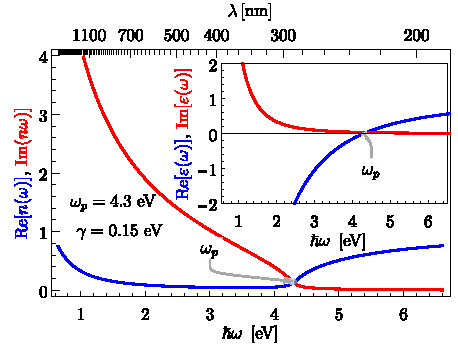
\includegraphics[scale=1]{1-Teoria/figs/1-4-varepsn4eV.pdf}
	\end{subfigure}\hspace*{.5em}
	\begin{subfigure}{.01\linewidth}\caption{}\label{sfig:Drude10eV}\vspace{3.75cm}\end{subfigure}
	\begin{subfigure}{.45\linewidth}\hspace*{-1em}
	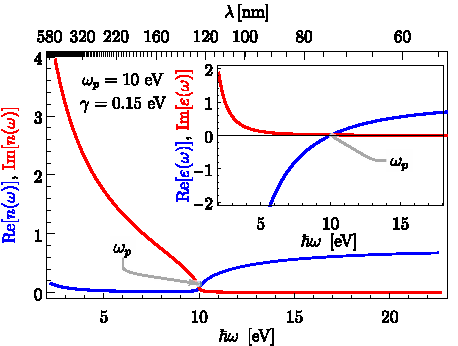
\includegraphics[scale=1 ]{1-Teoria/figs/1-4-varepsn10eV.pdf}
	\end{subfigure}\vspace*{-.7em}
	\caption{ Índice de refracción (gráfica externa) y función dieléctrica (gráfica interna) del modelo de Drude-Sommerfeld para las frecuencias de plasma \textbf{a)} $\hbar\omega_p=4. 3$ eV y \textbf{b)} $\hbar\omega_p=10$ eV; ambos casos con $\hbar\gamma=0. 15$ eV, como función de la energía.  En el marco superior se observa su dependencia con la longitud de onda $\lambda$. }\label{fig:Drude}
	\end{figure}	

\subsection{Corrección por tamaño para partículas esféricas}
\label{ssection:CorreccionTamano}

La corrección de la función dieléctrica para NPs esféricas a partir de la función dieléctrica de bulto $\varepsilon_B^{exp}(\omega)$, obtenida mediante métodos experimentales, consiste en la modificación de la constante fenomenológica de amortiguamiento en el modelo de Drude-Sommerfeld\footnote{También es posible hacer una corrección de tamaño en la contribución interbanda de la función dieléctrica considerando la densidad de estados. Sin embargo, para los datos experimentales de \cite{johnson1972constants}, esta corrección para partículas esféricas es apreciable para NPs con radios menores a $2$ nm \cite{mendoza2014determination}.}, dado que ésta depende del camino libre medio de los electrones $L$ y debe modificarse cuando el radio de las NPs $a$ es menor a $L$ \cite{kreibig1995clusters}. Por ejemplo, para metales típicos  como el oro y la plata, a frecuencias del espectro visible y a una temperatura de $273$ K, el camino libre medio de los electrones libres para el oro y la plata es  de $56$ nm  y $42$ nm, respectivamente\footnote{Cálculos a partir de los datos obtenidos de las tablas 1.3 y 2.1 de \cite{ashcroft1976solid}, donde $v_F^{Au} = 1.40\times 10^{15}$ nm s$^{-1}$ y $v_F^{Ag}=1.39\times 10^{15}$ nm s$^{-1}$.\index{Fermi!velocidad de}}, por lo que para NPs de oro o plata con radios menores a $60$ nm se hace una corrección de la constante fenomenológica para materiales de bulto. La corrección de $\gamma_B $ para una partícula esférica de radio $a$ se calcula al considerar el camino libre medio efectivo de los electrones, proporcional al radio de la partícula, obteniedo así un término de amortiguamiento adicional al de bulto y que es aditivo a éste \cite{kreibig1995clusters}, es decir,\index{Drude-Sommerfeld!modelo de!constante fenomenológica de amortiguamiento ($\gamma$)!para esferas ($\gamma_a$)}
%
	\begin{align*}
	 \gamma = \gamma_B+ \gamma_a = v_F \qty(\frac{1}{L}+\frac{A}{a}). 
	\end{align*}
%
donde $A$ es un parámetro del orden de la unidad \cite{noguez2007surface,mendoza2014determination} y depende de la teoría con la que se calcule el camino libro medio efectivo \cite{kreibig1995clusters}.  Entonces, para NPs esféricas modeladas por una función dieléctrica tipo Drude [Ec.  \eqref{eq:Drude}] se emplea  la corrección por tamaño de la función dieléctrica dada por \index{Función dieléctrica!para partículas esféricas, corrección por tamaño de la}
%
	\begin{align}
	\frac{\varepsilon(\omega)}{\varepsilon_0} = \frac{\varepsilon_B^{exp}(\omega)}{\varepsilon_0}
						 - \qty( 1 - \frac{\omega_p^2}{\omega(\omega+i\gamma_B)}) 
						 + \qty( 1 - \frac{\omega_p^2}{\omega[\omega+i(\gamma_B + Av_F/a)]}),
			\label{eq:sizeCorrection}
	\end{align}
%
en donde se resta la contribución del material de bulto  a la función dieléctrica experimental $ \varepsilon_B^{exp}(\omega)$ y se introduce la función dieléctrica con la corrección $\gamma = \gamma_B+\gamma_a$. Para realizar este proceso se calculan los parámetros $\omega_p$ y $\gamma_B$ que mejor ajusten el modelo de Drude-Sommerfeld a los datos experimentales, sin embargo, la función dieléctrica experimental del material $\varepsilon_B^{exp}(\omega)$ depende del método de fabricación de la muestra y del sustrato sobre el que está depositada \cite{svetovoy2008optical,raja2019dielectric}. En el cálculo de $\omega_p$ y $\gamma_B$ se debe considerar que el comportamiento tipo Drude es válido para el límite $\omega\to 0$ (caso estático), por lo que el ajuste debe hacerse hasta una cierta frecuencia de corte en la que el modelo de Drude aún sea válido \cite{mendoza2014determination}, y la elección de la frecuencia de corte para el ajuste modifica el resultado de los parámetros de Drude.

Para determinar los parámetros $\omega_p$ y $\gamma$ del modelo de Drude [Ec. \eqref{eq:Drude}] se emplea el método propuesto en \cite{mendoza2014determination}, donde se construyen dos relaciones lineales entre $\varepsilon'(\omega) = \Re[\varepsilon_D(\omega)/\varepsilon_0]$ y $\varepsilon''(\omega)=\Im[\varepsilon_D(\omega)/\varepsilon_0]$. Las partes real e imaginaria de la Ec. \eqref{eq:Drude} son%  \vspace*{-1em}

	\begin{subequations}\eqhalf{\varepsilon' =
		 1 - \frac{\omega_p^2 \omega^2}{\omega^4 + (\omega\gamma)^2},
		 \label{eqs:ReDrude}}
	\eqhalf{\varepsilon'' =
		 \frac{\omega_p^2  (\omega\gamma)}{\omega^4 + (\omega\gamma)^2},
		 \label{eqs:ImDrude}
			}\end{subequations} 
			
\noindent		
donde no se escribe la dependencia en $\omega$ de $\varepsilon'$ y $\varepsilon''$ para hacer más claro el siguiente procedimiento. Dado que $1-\varepsilon' = \omega_p^2\omega^2 / [\omega^4 + (\omega\gamma)^2]$, al calcular  $(1-\varepsilon')\gamma/\omega$ y sustituir con la Ec. \eqref{eqs:ImDrude} se obtiene que $	( 1-\varepsilon') (\gamma/\omega)=\varepsilon''$, por lo que se cumple la relación
%
	\begin{align}
	\omega\varepsilon''= \gamma( 1-\varepsilon'). \label{eq:gammaAjuste}
	\end{align}
%
Asimismo, al calcular la suma del cuadrado de $1-\varepsilon'$ y el cuadrado de $\varepsilon''$ se obtiene
%
	\begin{align*}
	( 1-\varepsilon') ^2 + (\varepsilon'')^2 
					=\frac{\omega_p^4 \omega^4}{[\omega^4 + (\omega\gamma)^2]^2}+
									\frac{\omega_p^4 (\omega\gamma)^2}{[\omega^4 + (\omega\gamma)^2]^2}
					= \frac{\omega_p^4[\omega^4 + (\omega\gamma)^2]}{[\omega^4 + (\omega\gamma)^2]^2}
					= \frac{\omega_p^4}{\omega^4 + (\omega\gamma)^2},
		\end{align*}
%
y al multiplicar ambos lados de la ecuación por $\omega^2$	 y sustituir con la Ec. \eqref{eqs:ReDrude} se obtiene
%
	\begin{align}
	\omega^2\qty[( 1-\varepsilon') ^2 + (\varepsilon'')^2 ]  
						= \omega_p^2( 1-\varepsilon').
	\label{eq:omegaAjuste}
	\end{align}
%
Es decir, al graficar el lado izquierdo de las Ecs. \eqref{eq:gammaAjuste} y \eqref{eq:omegaAjuste} como función de $ 1-\varepsilon'$ se obtienen dos funciones lineales sin ordenada al origen por lo que, al emplear los valores experimentales de la función dieléctrica, cuando estos no correspondan a una recta que cruza por el origen, la función dieléctrica deja de ser descrita por el modelo de Drude. Asimismo, es posible determinar los parámetros $\omega_p$ y $\gamma$ de la función dieléctrica empleando los valores de la parte real y la parte imaginaria de $\varepsilon(\omega)/\varepsilon_0$.

En la Fig.  \ref{fig:FitDrude} se muestran las gráficas de las Ecs. \eqref{eq:gammaAjuste} en rojo y \eqref{eq:omegaAjuste} en azul, donde se emplearon los datos experimentales para la función dieléctrica del oro [Fig. \ref{sfig:FitDrudeAu}] y la plata [\ref{sfig:FitDrudeAg}] obtenidos de \cite{johnson1972constants}. Para ambos materiales, el modelo de Drude-Sommerfeld describe los datos experimentales para $\hbar\omega<1.76$ eV (delimitado por la línea vertical gris); los datos considerados para el ajuste se muestran como anillos, el resto como discos. Mediante un ajuste de los datos experimentales, se determinó que para el oro $\hbar\omega_p=(8.70\pm 0.02)$ eV y $\hbar\gamma = (8.29\pm 0.08)\times 10^{-2}$ eV, mientras que para la plata $\hbar\omega_p=(9.05\pm 0.02)$ eV y $\hbar\gamma = (2.04\pm 0.08)\times 10^{-2}$ eV.

	\begin{figure}[h!]\centering\hspace*{-1.5em}
	\begin{subfigure}{.01\linewidth}\caption{}\label{sfig:FitDrudeAu}\vspace{3.75cm}\end{subfigure}
	\begin{subfigure}{.45\linewidth}\hspace*{-1.3em}
	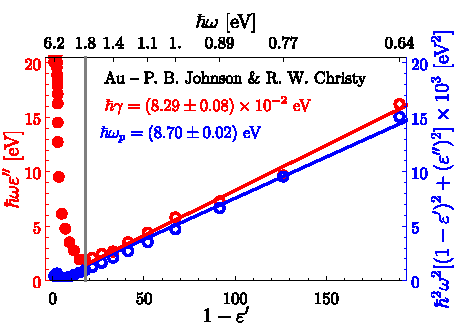
\includegraphics[scale=1]{1-Teoria/figs/1-4-DrudeFit_Au.pdf}
	\end{subfigure}
	\begin{subfigure}{.01\linewidth}\caption{}\label{sfig:FitDrudeAg}\vspace{3.75cm}\end{subfigure}
	\begin{subfigure}{.45\linewidth}\hspace*{-1em}
	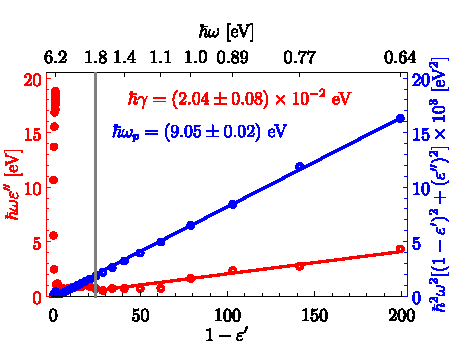
\includegraphics[scale=1]{1-Teoria/figs/1-4-DrudeFit_Ag.pdf}
	\end{subfigure}\vspace*{-.7em}
	\caption{ Determinación de los parámetros $\hbar\gamma$ (rojo) y $\hbar\omega_p$ (azul) mediante las Ecs. \eqref{eq:gammaAjuste} y \eqref{eq:omegaAjuste}, respectivamente, para los datos experimentales de la función dieléctrica \textbf{a)} del oro y \textbf{b)} la plata obtenidos de \cite{johnson1972constants}; la dependencia en la energía $\hbar\omega$ se muestra en la escala superior. Los anillos corresponden a datos considerados para el ajuste al modelo de Drude-Sommerfeld, mientras que los discos corresponden a los datos de contribuciones no plasmónicas; la división entre ambos regímenes corresponde a la línea vertical gris que para ambos casos se encuentra en $\hbar\omega\approx 1.76$ eV.}\label{fig:FitDrude}
	\end{figure}	

%	\begin{figure}[h!]\centering\hspace*{-1.5em}
%	\begin{subfigure}{.01\linewidth}\caption{}\label{sfig:sizeAu}\vspace{3.75cm}\end{subfigure}
%	\begin{subfigure}{.45\linewidth}\hspace*{-1.3em}
%	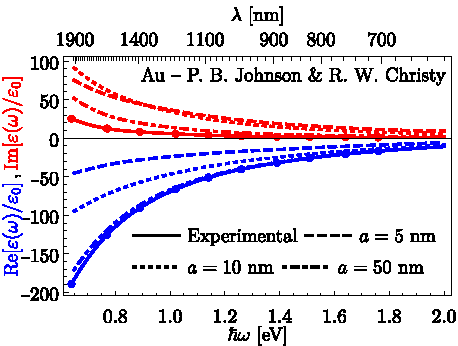
\includegraphics[scale=1]{1-Teoria/figs/1-4-sizeAuSmall.pdf}
%	\end{subfigure}
%	\begin{subfigure}{.01\linewidth}\caption{}\label{sfig:sizeAg}\vspace{3.75cm}\end{subfigure}
%	\begin{subfigure}{.45\linewidth}\hspace*{-1em}
%	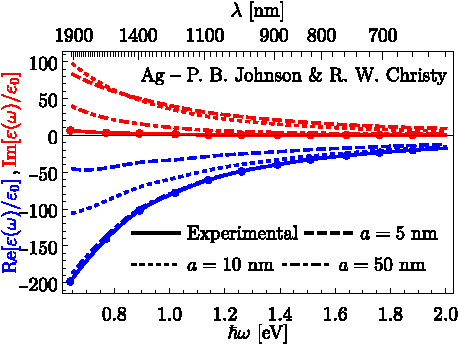
\includegraphics[scale=1]{1-Teoria/figs/1-4-sizeAgSmall.pdf}
%	\end{subfigure}\vspace*{-.7em}
%	\caption{ Comparación de la función dieléctrica como función de la energía $\hbar\omega$ para el\textbf{a)}  oro y \textbf{b)} la plata en bulto (líneas continuas) y para NPs esféricas de radio $a=5$ nm (líneas discontinuas), $a=10$ nm (líneas punteadas) y $a=50$ nm (líneas punto punteadas). La dependencia de la función dieléctrica con la longitud de onda $\lambda$ se muestra en el marco superior.}\label{fig:sizeCorrection}
%	\end{figure}	

%
%
%	\begin{figure}[h!]\centering
%	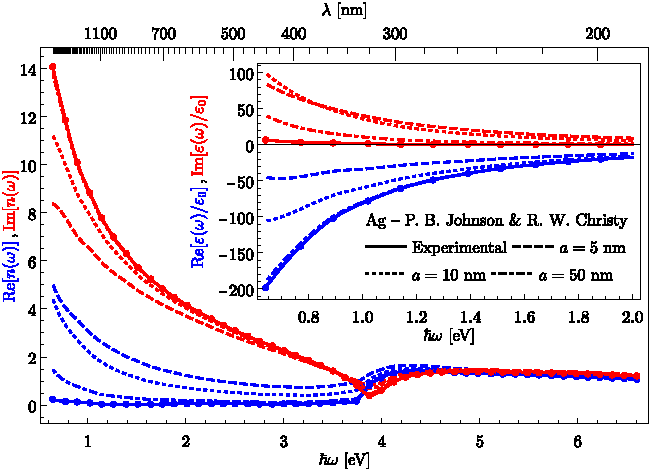
\includegraphics[scale=1]{1-Teoria/figs/0-sizeAgBig.pdf}
%    \vspace*{-1em}
%	\caption{ Comparación del índice de refracción (gráfica principal) y la función dieléctrica (gráfica secundaria) como función de la energía $\hbar\omega$ para el oro en bulto (líneas continuas) y para NPs esféricas de radio $a=5$ nm (líneas discontinuas), $a=10$ nm (líneas punteadas) y $a=50$ nm (líneas punto punteadas). La dependencia de la función dieléctrica con la longitud de onda $\lambda$ se muestra en el marco superior.}
%	\end{figure}		
%	
%	
%	\begin{figure}[h!]\centering
%	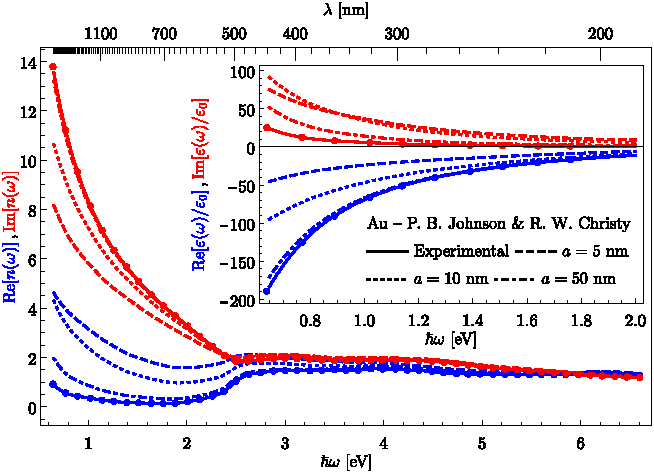
\includegraphics[scale=1]{1-Teoria/figs/0-sizeAuBig.pdf}
%    \vspace*{-1em}
%	\caption{Comparación del índice de refracción (gráfica principal) y la función dieléctrica (gráfica secundaria) como función de la energía $\hbar\omega$ para la plata en bulto (líneas continuas) y para NPs esféricas de radio $a=5$ nm (líneas discontinuas), $a=10$ nm (líneas punteadas) y $a=50$ nm (líneas punto punteadas). La dependencia de la función dieléctrica con la longitud de onda $\lambda$ se muestra en el marco superior.}
%	\end{figure}		

En la Fig.  \ref{fig:sizeCorrection} se muestra la correción por tamaño de la función dieléctrica del oro [Fig. \ref{sfig:sizeAu}] y la plata [Fig.  \ref{sfig:sizeAg}] para partículas esféricas, considerando $A=1$ en la Ec. \eqref{eq:sizeCorrection} \cite{noguez2007surface}. Tanto para el oro como para la plata, la función dieléctrica de bulto, experimental, corresponde a las líneas continuas y los puntos a sus valores experimentales; la función dieléctrica para NPs esféricas de radio $a=5$ nm corresponde a las líneas discontinuas; para $a=10$ nm, líneas punteadas; y para $a=50$ nm, líneas punto-discontinuas. Asimismo, para ambos materiales, la función dieléctrica para NPs se asemeja a la de bulto para energías $\hbar\omega>2$ eV. Sin embargo, para $\hbar\omega<2$ eV, los efectos de tamaño son apreciables y más significativos mientras menor sea el radio de las NPs, como se observa tanto  en la parte real (líneas azules) como en la imaginaria (líneas rojas) de la función dieléctrica, o con mayor claridad en las ampliaciones de la Fig. \ref{fig:sizeCorrection}, donde se muestra el comportamiento de la función dieléctrica del oro y de la plata en el espectro visible para distintos radios de NPs.\index{Función dieléctrica!del oro}\index{Función dieléctrica!de la plata}

	\begin{figure}[h!]\centering\hspace*{-1.5em}
	\begin{subfigure}{.01\linewidth}\caption{}\label{sfig:sizeAu}\vspace{7cm}\end{subfigure}
	\begin{subfigure}{.7\linewidth}\hspace*{-1em}
	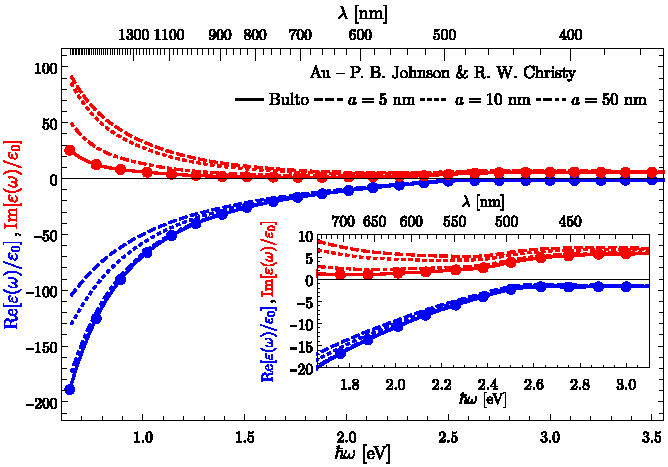
\includegraphics[scale=1]{1-Teoria/figs/0-sizeAuEpsilon.pdf}
	\end{subfigure}\\ \hspace*{-1.5em}
	\begin{subfigure}{.01\linewidth}\caption{}\label{sfig:sizeAg}\vspace{7cm}\end{subfigure}
	\begin{subfigure}{.7\linewidth}\hspace*{-1em}
	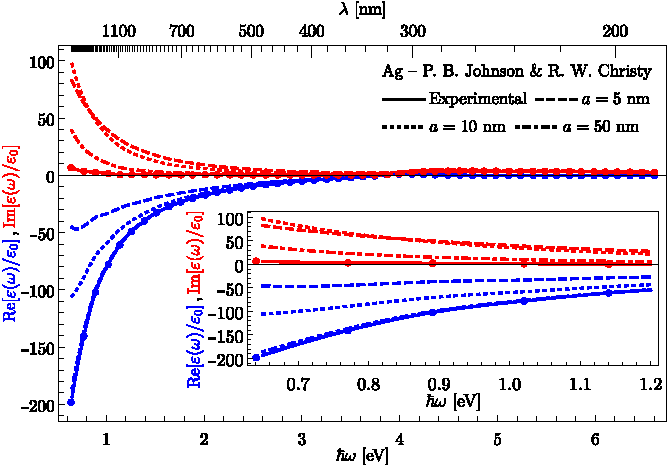
\includegraphics[scale=1]{1-Teoria/figs/0-sizeAgEpsilon.pdf}
	\end{subfigure}\vspace*{-.7em}
	\caption{Comparación de la función dieléctrica (parte real en azul e imaginaria en rojo) como función de la energía $\hbar\omega$ para \textbf{a)} el oro y \textbf{b)} la plata en bulto (líneas continuas) y para NPs esféricas de radio $a=5$ nm (líneas discontinuas), $a=10$ nm (líneas punteadas) y $a=50$ nm (líneas punto-discontinuas). La dependencia de la función dieléctrica con la longitud de onda $\lambda$ se muestra en la escala superior. Los datos experimentales para la función dieléctrica de bulto fueron tomados de \cite{johnson1972constants}, y se grafican como puntos en \textbf{a)} y en \textbf{b)}.}\label{fig:sizeCorrection}
	\end{figure}	

\subsection{Plasmones}
\label{ssection:Plasmones}

En la deducción de la función dieléctrica del modelo de Drude [Ec. \eqref{eq:Drude}] se resolvió la ecuación de movimiento de los electrones libres en un material ante la  presencia de un campo eléctrico oscilante en el tiempo. A las oscilaciones colectivas (modos propios) de los electrones libres debido al acoplamiento con la radiación EM se les denominan  plasmones, que pueden ocurrir en el bulto \cite{stockman2011nanoplasmonics}, o bien, sobre una superficie. A diferencia del plasmón de volumen, las resonancias plasmónicas de superficie (Surface Plasmon Resonances, SPRs) pueden clasificarse en modos propagantes y localizados. Cuando un plasmón se propaga a lo largo de una interfaz plana entre un medio diel\'ectrico y uno met\'alico, se le denomina  \emph{plasm\'on-polarit\'on de superficie} (Surface Plasmon Polariton, SPP) \cite{maier2007plasmonics}.  Si el plasmón, en cambio, se encuentra en la superficie de una partícula  met\'alica, de tamaño finito, se le conoce como \emph{resonancia de plasm\'on de superficie localizado} (Localized Surface Plasmon Resonance, LSPR) \cite{maier2007plasmonics}.\index{Plasmón}\index{Plasmón!Polaritón de Superficie (SPP)}\index{Plasmón!de Superficie Localizado, Resonancia de (LSPR)}

Para determinar a qué frecuencias se excitan los plasmones de volumen se calcula el rotacional de la ley de Faraday-Lenz y se sustituye el rotacional del campo magnético con la ley de Ampère-Maxwell, y  tras calcular su transformada de Fourier el resultado es \cite{maier2007plasmonics}
%
	\begin{align*}
	\vb{k}(\vb{k}\cdot\vb{E})-k^2\vb{E} =
			 -\frac{\varepsilon(\omega)}{\varepsilon_0}
			 \frac{\omega^2}{c^2}\vb{E},
	\end{align*}
%
donde se hace la distinción entre los casos de ondas transversales ($\vb{k}\cdot\vb{E}=0$), obteniendo la relación de dispersión \index{Relación de dispersión}
%
	\begin{align*}
	k^2 = \frac{\varepsilon(\omega)}{\varepsilon_0}  \frac{\omega^2}{c^2},
	\tag{\ref{eq:dispersion} \emph{bis}}\label{eq:TMode}		
	\end{align*}
%
y los casos con ondas longitudinales ($\vb{k}\cdot\vb{E}=kE$), en donde
%
	\begin{align}
	\varepsilon(\omega) = 0.
	\label{eq:LMode}
	\end{align}
%
Para obtener la relación de dispersión de un plasmón de volumen, se sustituye la función dieléctrica del modelo de Drude-Sommerfeld [Ec. \eqref{eq:Drude}], considerando el límite $\gamma\to 0$, en las Ecs. \eqref{eq:TMode} y \eqref{eq:LMode}, dando como resultado\index{Relación de dispersión!del plasmón de volumen}\index{Plasmón! de volumen} \vspace*{-.75em}\begin{subequations}
%
	\begin{tcolorbox}[title = Relación de dispersión del plasmón de volumen,  breakable, ams align ]
%	\omega &=  \sqrt{(ck)^2+\omega_p^2}, & \mbox{(Modo transversal)}
	k^2 &= \frac{\omega^2-\omega_p^2}{c^2}, 	& \mbox{(Modo transversal)}\\
	\omega&=\omega_p.							& \mbox{(Modo longitudinal)}
	\label{eq:volumePlasmon}
	\end{tcolorbox}\end{subequations}\vspace*{-.75em}\noindent
%
Dado que el plasmón de volumen es un modo longitudinal no puede acoplarse a ondas EMs transversales \cite{maier2007plasmonics}. Por otro lado, el SPP sí responde a ondas EM transversales y su relación de dispersión se calcula al considerar la geometría presentada en la Fig. \ref{fig:SPP}, en donde un haz de luz incide sobre una interfaz plana entre un medio dieléctrico, con una función dieléctrica $\varepsilon_1(\omega)>0$ y uno metálico con $\varepsilon_2(\omega)$, es decir, que cumpla con que $\Re[\varepsilon_2(\omega)]<0$, que en el modelo de Drude-Sommerfeld [Ec. \eqref{eq:Drude}] basta con que $\omega<\omega_p$.

\begin{figure}[h!]\centering
	\begin{tikzpicture}[scale=1.2]
	%-------------------------------------------- Incidence media
\shadedraw[	top color = yellow,				%%%%	Color de arriba
			bottom color =yellow,				%%%%	Color de abajo
			middle color = white, 			%%	Color de en medio
			shading angle = 35]			%%%%	Ángulo de gradiente
		 (-4,-1) rectangle (4,0);
% Interface
\draw[yellow,line width=.5pt](-4,0)--(4,0)--(4,-1)--(-4,-1)--(-4,0); %%..5pt, interface]
% Media names
\node at (-2.75,.3) {Diel\'ectrico $\; \varepsilon_1(\omega)$}; 
\node at (-3,-.3) {Metal  $\; \varepsilon_2(\omega)$};
\node at (4.5,0) {$z=0$};

%-------------------------------------------- Laser beam outside
\draw[fill=red, opacity = 1,red](-2.25,2)--(-1.75,2)-- (0,.3)  %%% outside the metal
						--(1.75,2)--(2.25,2)
						--(.25,0)--(-.25,0)--(-2.25,2);																														
%--------------------------------------------  Incident Wave
\path (0,0)++(112.5:1cm)node{$\theta_i$};       % Angle
\draw[latex - latex](95:.75cm)arc(95:130:.75cm);
 
    \draw[- latex,line width=1pt](135:1.9cm)--(135:1.2cm);    %Wave vector
    \path (0,0)++(141:1.1cm)node[left]{$\vb{k}_i$};     %Wave vector label
    
%--------------------------------------------  Reflected Wave
\path (0,0)++(67.5:1cm)node{$\theta_r$};       % Angle
\draw[latex - latex](85:.75cm)arc(85:50:.75cm);
 
    \draw[- latex,line width=1pt](45:1.2cm)--(45:1.9cm);    %Wave vector
    \path (0,0)++(43:1.1cm)node[right]{$\vb{k}^r$};     %Wave vector label
  
%--------------------------------------------  Transmitted Wave & Skin depth
\draw[fill = red, opacity = .35] (-.25,0) ..controls (-.025,-.25) .. (0,-.75)
											..controls (.025,-.25) .. (.25,0);  %1st evanescent wave
\draw[fill = red, opacity = .35] (-.2,0) ..controls (-.075,-.125) .. (0.05,-.375)
											..controls (.075,-.125) .. (.3,0);  %2nd evanescent wave
\draw[fill = red, opacity = .35] (-.15,0) ..controls (-.025,-.0625) .. (0.1,-.1875)
											..controls (.175,-.0625) .. (.35,0);  %3rd evanescent wave
\draw[fill = red, opacity = .35] (-.1,0) ..controls (.025,-.03125) .. (0.15,-.09375)
											..controls (.225,-.03125) .. (.4,0);  %4th evanescent wave	

    \draw[- latex,line width=1pt](0,-.5)--(.9,-.5);    %Wave vector
    \node at (.6,-.8) {$\vb{k}_x$};
    
    \draw[|-|,line width=.2mm,black] (-.5,.0)--(-.5,-.75);%
    \node at (-1.25,-.4) {$\xi=\dfrac{1}{k_x}$};
%--------------------------------------------  Axes
\draw[latex - latex, line width =1pt] (0,2)node[left]{$z$}--(0,0) -- (2,0)node[right]{$x$};
\end{tikzpicture}
	\caption{ Esquema de una interfaz entre un medio dieléctrico ($z>0$) y uno metálico ($z<0$) sobre la que incide un haz de luz proveniente del medio dieléctrico; ambos  materiales son homogéneos, lineales e isótropos. La reflexión del haz de luz es total debido a la naturaleza metálica del material. Sin embargo, por las condiciones a la frontera de los campos EMs se presenta una onda evanescente en $z<0$ que se propaga en dirección de $\vb{k}_x$, paralela a la interfaz, y la longitud de penetración de la onda evanecente es $\xi=1/k_x$, con $k_x$ la magnitud de $\vb{k}_x$. }\label{fig:SPP}
	\end{figure}
	
En la Fig. \ref{fig:SPP} se observa que al incidir el haz de luz sobre la interfaz ($z=0$)  entre el medio dieléctrico ($z>0$) y el metálico ($z<0$), se presenta una onda evanescente en el medio metálico que se propaga en la dirección de $\vb{k}_x=k_x\vu{e}_x$, cuya amplitud decae exponencialmente en la dirección $\vu{e}_z$ y cuyo máximo valor $\xi=1/k_x$ es su longitud de penetración.\index{Plasmón!Polaritón de Superficie (SPP)!longitud de penetración ($\xi$)} Si se considera que una onda plana, con frecuencia $\omega$ y vector de onda $\vb{k}^i$, es la que incide sobre la interfaz, los campos EMs de la onda evanescente se proponen como \index{Onda!evanescente}

	\begin{subequations}\eqhalf{	\vb{E}(\vb{r},t) = \vb{E}(z)e^{ik_x x-\omega t },}
	\eqhalf{\vb{H}(\vb{r},t) = \vb{H}(z)e^{ik_x x-\omega t},}
	\label{eq:EHbetax}\end{subequations} \vspace*{-1em}
	
\noindent donde $\vb{E}(z>0)=\vb{E}_1$, con $E_1$ la magnitud del campo eléctrico dentro del dieléctrico, y $\vb{E}(z<0)=\vb{E}_2$ la magnitud del campo eléctrico en el medio metálico; lo análogo se cumple para el campo $\vb{H}$ y para la función dieléctrica $\varepsilon(z)$. La ecuación de Helmholtz [Ecs. \eqref{eq:Helmholtz}] para los campos EMs de las Ecs. \eqref{eq:EHbetax} son

	\begin{subequations}
	\eqhalf{	\pdv[2]{\vb{E}}{z} + \qty[k_0^2\frac{\varepsilon(z)}{\varepsilon_0} - k_x^2 ] \vb{E}= 0,\label{eq:helmE}}
	\eqhalf{\pdv[2]{\vb{H}}{z} + \qty[k_0^2\frac{\varepsilon(z)}{\varepsilon_0}  - k_x^2 ] \vb{H}= 0, \label{eq:helmH}}
	\end{subequations} 
	
\noindent con $k_0 = \omega/c$. Para el cálculo de la relación de dispersión del SPP, se considera que existe homogeneidad en la dirección $y$, y que la única dependencia en la variable $x$  es en el término de propagación, es decir, que $\partial/\partial x\to ik_x$. Bajo estas consideraciones, al desarrollar la ley de Faraday-Lenz y la ley de Ampère-Maxwell con las expresiones de las Ecs. \eqref{eq:EHbetax}, se obtiene el siguiente conjunto de ecuaciones \vspace*{-1em}

	\begin{subequations}
	\eqhalf{	\mqty(-\pdv*{E_y}{z} \\ \pdv*{E_x}{z}-ik_x E_z\\ik_x E_y)
				= i\omega\mu_0 \mqty(H_x\\H_y\\h_z),}
	\eqhalf{	\mqty(-\pdv*{H_y}{z} \\ \pdv*{H_x}{z}-ik_x H_z\\ik_x H_y)
				= i\omega\varepsilon(z) \mqty(E_x\\E_y\\E_z).}	
	\end{subequations}\noindent 

El SPP es sensible a la polarización de la onda plana incidente por lo que se consideran los casos de polarización \emph{s} y \emph{p}. En polarización \emph{s}, las componentes no nulas de los campos EMs son $E_y$, $H_z$ y $H_x$, por lo que se  cumplen las relaciones

	\begin{subequations}
	\eqhalf{	H_x =  \frac{i}{\omega \mu_0} \pdv{E_y}{z},\label{eq:Hx}}
	\eqhalf{H_z =  \frac{k_x}{\omega \mu_0} E_y, \label{eq:Hz}}	
	\label{eq:ondaS}	\end{subequations} \vspace*{-1em}

\noindent junto con la ecuación de Helmholtz para el campo eléctrico [Ec. \eqref{eq:helmE}] con  $\vb{E} = E_y\vu{e}_y$, cuya solución se propone como
%
	\begin{align}
	E_y(z) = \begin{dcases}
		E_1 e^{ik_x x} e^{-k_{1,z}z}, & z>0\\
		E_2 e^{ik_x x} e^{k_{2,z} z}, & z<0
		\end{dcases},\label{eq:AnsatzEy}
	\end{align}
%	
con $k_{j,z} = k_j\cos\theta_i$ y $k_j = k_0 \sqrt{\varepsilon_j(\omega)/\varepsilon_0}$, con $j = 1,2$; donde se escribe de forma explícita el comportamiento del decaimiento exponencial en la amplitud y se omite el término $e^{-i\omega t}$ por simplicidad. Al calcular el campo $\vb{H}$ con las Ecs. \eqref{eq:ondaS} y \eqref{eq:AnsatzEy}, se obtienen las expresiones 
	
	\eqhalf{	H_x(z) = \begin{dcases}
	-i \frac{E_1}{\omega\mu_0}k_{1,z} e^{ik_x x} e^{-k_{1,z} 	z}, & z>0\\
	i \frac{E_2}{\omega\mu_0}k_{2,z} e^{ik_x x} e^{k_{2,z} z}, & z<0
	\end{dcases},\notag}
	\eqhalf{	H_z(z) = \begin{dcases}
	\frac{E_1}{\omega\mu_0}k_x  e^{ik_x x} e^{k_{1,z} z} & z>0\\
	\frac{E_2 }{\omega\mu_0}k_x  e^{ik_x x} e^{k_{2,z}z} & z<0
	\end{dcases}.\notag}
	
\noindent   Las condiciones a la frontera impuestas en los campos EMs resultan en que las componentes paralelas a la interfaz del campo eléctrico, $E_y$, y del campo $\vb{H}$, $H_z$, sean continuas, por lo que $E_1 = E_2$. Adicionalmente, por la continuidad de la componente paralela a la interfaz del  campo $\vb{H}$, $H_x$, se concluye que en $z=0$
%
	\begin{align}
	E_1\qty(k_{1,z}+k_{2,z})= 0. \label{eq:condS}
	\end{align}
%
Por el \emph{Ansatz} propuesto en la Ec. \eqref{eq:AnsatzEy}, para que la onda evanescente esté confinada a la interfaz se debe cumplir que $k_{j,z}<0$, por tanto la Ec. \eqref{eq:condS} se satisface sólo si $E_1 = E_2 = 0$, es decir  que no existe un acoplamiento entre los electrones libres del metal en la interfaz plana y la onda EM incidente para polarización \emph{s}.

El cálculo de la relación de dispersión del SPP para polarización \emph{p} es análogo al cálculo con polarización \emph{s} al intercambiar el campo eléctrico por el campo $\vb{H}$ y al intercambiar la permeabilidad magnética por la función dieléctrica \cite{maier2007plasmonics}, es decir, $\vb{E}\leftrightarrow\vb{H}$ y $\varepsilon(z)\leftrightarrow\mu_0$. Al considerar las condiciones de continuidad del campo $\varepsilon(z)\vb{E}$ y el campo $\vb{H}$, se obtiene la expresión
%
	\begin{align*}
	\frac{E_1}{\omega}\qty( \frac{k_{1,z}}{\varepsilon_1}+  \frac{k_{2,z}}{\varepsilon_2} ) = 0,
	\end{align*}
%
de donde se obtiene que
%
	\begin{align}
	\frac{k_{1,z}}{k_{2,z}} = - \frac{\varepsilon_1}{\varepsilon_2}. \label{eq:condP}
	\end{align}
%
Asimismo, la ecuación de Helmholtz para el campo $\vb{H}$ [Ec. \eqref{eq:helmH}] impone que
%
	\begin{align}
	k_{j,z}^2 = k_x^2 - k_0^2 \frac{\varepsilon_j}{\varepsilon_0}.
	\label{eq:kdkm}
	\end{align}
%
Al elevar al cuadrado ambos lados de la Ec. \eqref{eq:condP}, sustituir $k_{j,z}^2$ con la Ec. \eqref{eq:kdkm}, y  despejar $k_x^2$  empleando la identidad de diferencia de cuadrados,  se calcula la relación de dispersión del SSP. Adicionalmente, como  $k_0^2 \varepsilon_j(\omega)= k_x^2 +k_{j,z}^2$, entonces \cite{maier2007plasmonics}\index{Plasmón!Polaritón de Superficie (SPP)}\index{Relación de dispersión!del SPP|see {Plasmón}}\vspace*{-.75em}\begin{subequations}
%
	\begin{tcolorbox}[title = Relación de dispersión del SPP, breakable ]
	\eqhalf{k_x^2 = \frac{k_0^2}{\varepsilon_0} \frac{\varepsilon_1 \varepsilon_2}{\varepsilon_1 + \varepsilon_2},
	\label{eqs:kx}}
	\eqhalf{	k_{j,z}^2 = \frac{k_0^2}{\varepsilon_0} \frac{\varepsilon_j^2}{\varepsilon_1 + \varepsilon_2},\label{eqs:kz}}
	
	con $j=1$ para el medio dieléctrico y $j=2$ para el medio metálico.
	\end{tcolorbox}\label{eq:SPPRelDiso}\end{subequations}\vspace*{-.75em}\noindent
%	
Para que se obtenga una onda evanescente en la interfaz (modo ligado), $k_x$ debe ser una cantidad real y $k_z$ una cantidad imaginaria \cite{novotny2006principles}, por lo que en la Ec. \eqref{eqs:kx} la suma y el producto de las funciones dieléctricas deben ser ambas positivas o ambas negativas y $\varepsilon_1+\varepsilon_2<0$ en la Ec. \eqref{eqs:kz} \cite{novotny2006principles}, dando como resultado que $\varepsilon_1\varepsilon_2<0$. Estas condiciones se satisfacen con la suposición inicial en la que $\varepsilon_1$ corresponda a la respuesta EM de un medio dieléctrico y $\varepsilon_2$ a la de un metal \cite{novotny2006principles,maier2007plasmonics}. La frecuencia de resonancia $\omega$ del SPP se obtiene maximizando las Ecs. \eqref{eq:SPPRelDiso}, es decir, cuando $\varepsilon_1(\omega)+\varepsilon_2(\omega)$ es mínima. Si se emplea el modelo de Drude-Sommerfeld [Ec. \eqref{eq:Drude}] en el límite $\gamma\to 0$ para $\varepsilon_2(\omega)$, entonces \cite{maier2007plasmonics}  \vspace*{-.75em}
	\begin{tcolorbox}[title =Frecuencia de resonancia del SPP, ams align,  breakable ]
	\omega = \frac{\omega_p}{\sqrt{1+\varepsilon_1/\varepsilon_0}}.
	\end{tcolorbox}\vspace*{-.75em}\noindent

La Fig. \ref{fig:Relaciones_de_dispersion} muestra la relación de dispersión como la dependencia de la frecuencia $\omega$ con la componente paralela del vector de onda $k_x$, respecto a una interfaz entre el vacío ($\varepsilon_1=\varepsilon_0$) y un material descrito por el modelo de Drude-Sommerfeld [Ec. \eqref{eq:Drude}], en el límite $\gamma\to 0$ para una onda plana monocromática propagándose en el vacío (línea continua negra), para el plasmón de volumen (línea continua roja) y para un SPP (línea continua azul). Las líneas discontinuas roja y azul corresponden a los valores $\omega=\omega_p$ y $\omega=\omega_p/\sqrt{2}$, respectivamente, que son las frecuencias que delimitan el régimen de modos radiativos ($\omega>\omega_p$), donde las dos componentes del vector de onda $\vb{k}$ son cantidades reales, y el régimen de modos ligados ($\omega<\omega_p/\sqrt{2}$), donde $k_x$ es una cantidad real pero la componente del vector de onda perpendicular a la interfaz $k_z$ es una cantidad imaginaria. La línea discontinua negra corresponden a la relación de dispersión de una onda plana monocromática propagándose  en un medio con $n=1.5$.\index{Relación de dispersión}

\begin{figure}[h!]\centering
	\begin{tikzpicture}
	\node[inner sep=0pt] at (0,0)
    {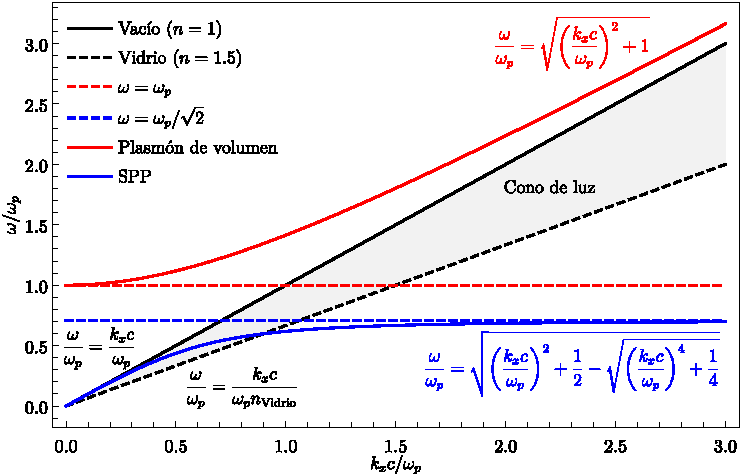
\includegraphics[scale=1]{1-Teoria/figs/1-4-RelacionDispersion.pdf}};
    \draw [thick, decorate, decoration={brace,amplitude=10pt,mirror}]
(6.5,-.8) -- (6.5,4.0);
\node at (8,2.5){\footnotesize Modo};
\node at (8,2.){\footnotesize radiativo};
\node at (8,1.5){\footnotesize $k_x\to\text{Real}$};
\node at (8,1.){\footnotesize $k_z\to\text{Real}$};
    \draw [thick, decorate, decoration={brace,amplitude=10pt,mirror}]
(6.5,-3.25) -- (6.5,-1.3);
\node at (8,-1.5){\footnotesize Modo};
\node at (8,-2.){\footnotesize ligado};
\node at (8,-2.5){\footnotesize $k_x\to\text{Real}$};
\node at (8,-3.){\footnotesize $k_z\to\text{Imaginario}$};
\end{tikzpicture}
\vspace*{-.5em}
	\caption{Relación de dispersión en términos de $\omega/\omega_p$ como función de $k_xc/\omega_p$ de una onda plana monocromática en vacío (línea sólida negra), del plasmón de volumen (línea sólida roja) y del SPP (línea sólida azul) para materiales con una función dieléctrica tipo Drude en el límite $\gamma\to 0$, considerando una interfaz entre estos materiales y el vacío ($\varepsilon_1 =\varepsilon_0$). El régimen de modos radiativos se encuentra en $\omega_p\leq\omega$ (igualdad denotada por la línea discontinua roja), donde $k_x$ y $k_z$ son cantidades reales; el régimen de modos ligados se encuentra en $\omega\leq\omega_p/\sqrt{2}$ (igualdad denotada por la línea discontinua azul), donde $k_x$ es una cantidad real pero $k_z$ es una cantidad imaginaria. Para excitar a un SPP es necesario cambiar el índice de refracción de la matriz, por ejemplo empleando un prisma para obtener una onda plana viajando en vidrio (línea punteada negra); la región sombreada delimita las frecuencias a las que el SPP puede excitarse.}
	\label{fig:Relaciones_de_dispersion}
	\end{figure}		

La relación dispersión de la onda plana monocromática propagándose en el vacío (línea continua negra en la Fig. \ref{fig:Relaciones_de_dispersion})  es igual a la del SPP (línea continua azul) para  $k_x=0$, por lo que no es posible excitar al SPP con este tipo de ondas \cite{trugler2011properties}. Sin embargo, un arreglo experimental que permite excitar al SPP sobre la interfaz entre un medio dieléctrico, con función dieléctrica $\varepsilon_1(\omega)$, y una película  metálica, caracterizada por $\varepsilon_2(\omega)$ y de grosor $d$, consiste en soportar la película metálica sobre un sustrato, con una función dieléctrica $\varepsilon_3(\omega)>\varepsilon_1(\omega)$, e iluminarla en una configuración de reflexión total atenuada (Attenuated Total Reflection, ATR) \cite{kabashin2009plasmonic,trugler2011properties}\index{Reflexión total!atenuada}, como se muestra en la Fig. \ref{sfig:ATR}. En este tipo de configuración se emplea el sustrato para generar una onda evanescente en la interfaz entre éste y la película metálica que logre penetrar hasta la interfaz entre la película metálica y el dieléctrico con $\varepsilon_1(\omega)$. Cuando una onda plana monocromática incide sobre la interfaz entre la película metálica y el sustrato, con un ángulo de incidencia mayor al ángulo crítico, se produce una onda evanescente que se propaga en la dirección $\vb{k}_x=k_x\vu{e}_x$ y si $\xi=1/k_x>d$, la onda evanescente penetra la interfaz entre la matriz y la película, excitando al SPP \cite{trugler2011properties}, representado por la línea naranja en la Fig. \ref{sfig:ATR}. En la Fig. \ref{sfig:SPP-R} se grafica la reflectancia $R$ como función del ángulo de incidencia $\theta_i$, de la longitud de onda $\lambda$ y la energía $\hbar\omega$ de la onda plana, cuando ésta se propaga a través del prisma, con $\varepsilon_3(\omega)/\varepsilon_0 = 1.5^2$, e incide sobre una película de oro de grosor $d=50$ nm que forma una interfaz con el vacío ($\varepsilon_1(\omega)/\varepsilon_0 = 1$). Para $\lambda<500$ nm la reflectancia es cercana a cero pues el oro se comporta como un dieléctrico, mientras que para $\lambda>500$ nm tiene una respuesta metálica por lo que la reflexión de luz aumenta; para $\theta_i>42^\circ$ la luz que incide sobre la placa metálica se refleja totalmente a excepción de una región resaltada por la línea punteada blanca, para la cual $R\approx 0$ en $\lambda>500$ nm, que  corresponde a las combinaciones de ángulo de incidencia y longitudes de onda ---equivalente a valores de $k_x$ y $\omega$, respectivamente--- a los que el SPP se propaga sobre la interfaz entre la película de oro y el vacío.
			
	\begin{figure}[h!]\centering
	\begin{subfigure}{.01\linewidth}\caption{}\label{sfig:ATR}\vspace{5cm}\end{subfigure}
	\begin{subfigure}{.45\linewidth}\hspace*{-1.5em}
		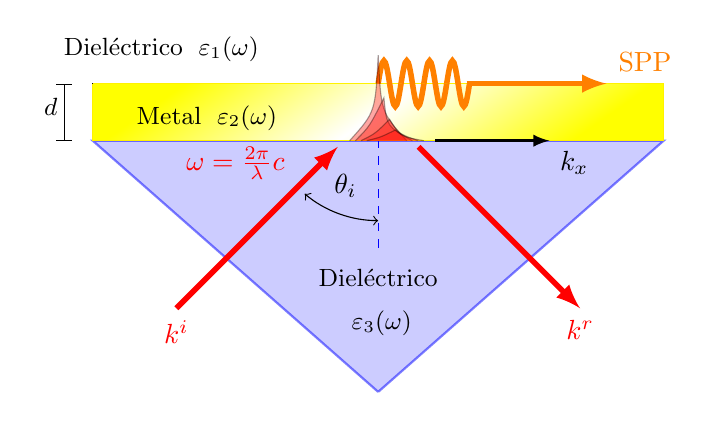
\begin{tikzpicture}[scale= 1.45]
	%-------------------------------------------- Incidence media
\def\a{.3}
\def\d{.3}
\def\dd{.2}
\def\l{2.5}
\def\ll{.05}

\fill[blue, opacity = .2] (0,-\l)--(\l,-\d)--(-\l,-\d);
\draw[blue, opacity = .5,thick] (0,-\l)--(\l,-\d)--(-\l,-\d)--(0,-\l);


\draw[|-|](-\l-.25,-\d)--(-\l-.25,+\dd);
\node at (-\l-.4,0) {\small $\;d$};
\draw[blue, dashed] (0,0)--(0,-\l*.5);

\path (0,0)++(-90-45*.5:\l*.3)node{$\theta_i$};       % Angle
\draw[<->](-90:\l*.4)arc(-90:-90-45*.89:\l*.4);

%\foreach \x in {-4,-2.9,-1,.1,1.2,2.4,3.8}{
%\fill[ball color=yellow, opacity=1] (\x,0) circle(\a);}

\shadedraw[	top color = yellow,				%%%%	Color de arriba
			bottom color =yellow,				%%%%	Color de abajo
			middle color = white, 			%%	Color de en medio
			shading angle = 35]			%%%%	Ángulo de gradiente
		 (-\l,-\d) rectangle (\l,\dd);
% Interface
\draw[yellow,line width=.5pt](-\l,\dd)--(\l,\dd)--(\l,-\d)--(-\l,-\d)--(-\l,\dd); %%..5pt, interface]

% Media names
\node at (0,-1.5) {\small Diel\'ectrico}; 
\node at (0,-1.9) {\small $\; \varepsilon_3(\omega)$}; 
\node at (-1.5,-.1) {\small Metal  $\; \varepsilon_2(\omega)$};
\node at (-1.9,.5) {\small Diel\'ectrico $\; \varepsilon_1(\omega)$}; 


\draw[latex -, thick, red, line width = 2](225:.5)--(225:2.5) node[anchor= north]{$\vb{k}^i$};
\node at (-1.25,-.5) {\color{red} $\omega =\frac{2\pi}{\lambda}c$};
\draw[- latex, thick, red, line width= 2](-45:.5)--(-45:2.5)node[anchor=north ]{$\vb{k}^r$};
\draw[- latex, thick,   line width = 1](.5,-\d)--(1.5,-\d) node[anchor= north west ]{$\vb{k}_x$};

\foreach \i in {0,4,8,12}{
\draw[thick, orange,line width = 2,] (\i*\ll,\dd) sin (\i*\ll+\ll,\dd*2) cos (\i*\ll+2*\ll,\dd) sin (\i*\ll+3*\ll,0) cos (\i*\ll+4*\ll,\dd);
}
\draw[- latex, thick, orange,  line width = 2](15.5*\ll,\dd)--(2,\dd) node[anchor= south west ]{SPP};



\draw[fill = red, opacity = .35] (-.25,-\d) ..controls (-.025,.25-\d) .. (0,.75-\d)
											..controls (.025,.25-\d) .. (.25,-\d);  %1st evanescent wave
\draw[fill = red, opacity = .35] (-.2,0-\d) ..controls (-.075,.125-\d) .. (0.05,.375-\d)
											..controls (.075,.125-\d) .. (.3,0-\d);  %2nd evanescent wave
\draw[fill = red, opacity = .35] (-.15,0-\d) ..controls (-.025,.0625-\d) .. (0.1,.1875-\d)
											..controls (.175,.0625-\d) .. (.35,0-\d);  %3rd evanescent wave
\draw[fill = red, opacity = .35] (-.1,0-\d) ..controls (.025,.03125-\d) .. (0.15,.09375-\d)
											..controls (.225,.03125-\d) .. (.4,0-\d);  %4th evanescent wave	


\end{tikzpicture}	
\end{subfigure}\hspace*{1em}
\begin{subfigure}{.01\linewidth}\caption{}\label{sfig:SPP-R}\vspace{5cm}\end{subfigure}
	\begin{subfigure}{.45\linewidth}\hspace*{-1em}
%	\includegraphics[scale=1]{1-Teoria/figs/SPP.png}%
%	\includegraphics[scale=1, trim={00 -30 00 00}, clip]{1-Teoria/figs/0-RBar_v}
%	
\begin{tikzpicture}
\node[inner sep=0pt] (graf) at (-.1,0){\includegraphics[scale=1]{1-Teoria/figs/SPP.png}};
\node[right, inner sep=0pt] (legend) at (2.75,.05) {\includegraphics[scale=1, trim={00 -15 00 00}, clip]{1-Teoria/figs/0-RBar_v}};
\end{tikzpicture}\vspace*{-.5em}	
	
	\end{subfigure}\hfill	\vspace*{-.5em}
	\caption{\textbf{a)} Esquema de una configuración ATR para la medición de la relación de dispersión del SPP mediante la reflectancia $R$ y \textbf{b)}  cálculo de la reflectancia al considerar una película de oro de grosor $d=50$ nm con una función dieléctrica $\varepsilon_2(\omega)$, dada por los datos experimentales de \cite{johnson1972constants}, inmersa en una matriz dieléctrica con $\varepsilon_1(\omega)/\varepsilon_0 = 1$ y sobre un prisma dieléctrico con $\varepsilon_3(\omega)/\varepsilon_0=1.5^2$. Cuando una onda plana monocromática con polarización \emph{p} incide sobre la interfaz entre el prisma y la película de oro a un ángulo mayor al crítico se produce una onda evanescente propagante en la dirección $\vb{k}_x=k_x\vu{e}_x$; si la longitud de penetración $1/k_x$ es mayor al grosor $d$ de la película metálica, es posible excitar al SPP sobre la interfaz entre el medio metálico y la matriz, como se observa en la Fig. \ref{fig:Relaciones_de_dispersion}. La línea punteada blanca en \textbf{b)} corresponden a la relación de dispersión del SPP propagándose sobre la interfaz entre el aire y una película metálica de oro.}\label{fig:ATR-SPP}
	\end{figure}			
		
Los SPPs son ondas electromagnéticas propagantes acopladas a los electrones libres de un metal sobre una interfaz plana e infinita entre el metal y un medio dieléctrico \cite{maier2007plasmonics}. Cuando la interfaz  entre el medio metálico y el dieléctrico tiene una área finita, como sucede con NPs, el resultado de la interacción entre una onda plana incidente y los electrones libres del metal es una excitación no propagante, también causada por el acoplamiento entre la radiación EM y los electrones libres, denominada resonancia de plasmón de superficie localizado (Localized Surface Plasmon Resonance, LSPR) \cite{maier2007plasmonics}\index{Plasmón!de superficie localizado, resonancia de (LSPR)}. La curvatura de las NPs tiene dos efectos en las LSPRs: la amplificación de los campos EMs dentro y fuera de la NP  (campo cercano) y la excitación de la LSPR con iluminación directa, es decir, sin emplear métodos como la iluminación en ATR \cite{maier2007plasmonics}.

En presencia de una NP esférica iluminada por una onda plana monocromática, los campos EMs fuera de la NP corresponden a la suma de los campos EMs de la onda plana incidente ($\vb{E}^i$, $\vb{H}^i$) y de los campos EMs esparcidos por la NP ($\vb{E}^s$, $\vb{H}^s$), por lo que el vector de Poynting [Ec. \eqref{eq:Poynting}], al considerar su promedio temporal, puede escribirse como \cite{bohren1998absorption}
%
\begin{align*}
\langle\vb{S}\rangle_t 
		= \underbrace{\frac12 \Re \qty(\vb{E}^i\times\vb{H}^{i*})}_{\text{\normalsize $\langle\vb{S}^i\rangle_t $}} + 
		\underbrace{\frac12 \Re \qty(\vb{E}^s\times\vb{H}^{s*})}_{\text{\normalsize $\langle\vb{S}^s\rangle_t $}}+
		\underbrace{	\frac12 \Re\qty(\vb{E}^i\times\vb{H}^{s*} + \vb{E}^s\times\vb{H}^{i*})}_{\text{\normalsize$\langle\vb{S}^{ext}\rangle_t $}},
\end{align*}
%
en donde $\vb{S}^i$ y $\vb{S}^s$ son los vectores de Poynting correspondientes a la onda plana incidente, con número de onda $k_m$ y cuyo campo eléctrico tiene amplitud $E_0$, y a los campos EMs esparcidos por la NP, respectivamente, y $\vb{S}^{ext}$ corresponde a los productos cruzados. La energía $W_{abs}$ trasportada por los campos EMs que es absorbida por la partícula se calcula al integrar $\langle\vb{S}\rangle_t$ sobre una esfera de radio $R$ concéntrica a la NP, cuyo radio sea mayor al radio de la NP, es decir,
%
\begin{equation}
W_{abs} = - \int_0^{2\pi}\int_0^{\pi}
		\qty(\langle\vb{S}^i\rangle_t +\langle\vb{S}^s\rangle_t 
				+\langle\vb{S}^{ext}\rangle_t )
		\cdot \vu{e}_r \,\dd a
		 = W_i-W_{sca}+W_{ext},
		 \label{eq:WaAll}
\end{equation}
%
donde $W_i = 0$, pues se asume que la matriz donde se encuentra inmersa la NP no es absorbente \cite{bohren1998absorption}. Como $W_{abs}$ es independiente de $R$, al suponer que tanto la matriz como la NP no son magnéticas, es posible emplear la solución de Mie para la expresión de $\vb{E}^s$ en el campo lejano dada por las Ecs. \eqref{eq:EHsFF} y a partir de éstas calcular $\vb{H}^s$ con ley de Faraday-Lenz [Ec. \eqref{seq:FLArm}], dando como resultado que $W_{sca}$ es \cite{bohren1998absorption}
%
 	\begin{equation}
W_{sca} = \frac{\pi\norm{E_0}^2}{\omega\mu_0 k_m}
		\sum_\ell^\infty (2\ell+1)\Re(-i\xi_\ell^*\xi_\ell')\qty(\abs{a_\ell}^2+\abs{b_\ell}^2),
	\label{eq:WsAll}
	\end{equation}
%
en donde $a_\ell$ y $b_\ell$ son los coeficientes de Mie [Ecs.  \eqref{eq:MieCoef}], $\xi_\ell(\rho) = \rho h_\ell^{(1)}(\rho)$ es una función de Riccati-Bessel, y donde además se emplearon las propiedades de ortogonalidad de las funciones $\sin\varphi$ y $\cos\varphi$ [Ec. \eqref{eq:ortSinCos}], de $\tau_\ell\pm\pi_\ell$ [Ec. \eqref{eq:ortTauPi}], junto con la relación \cite{bohren1998absorption}
%
	\begin{equation*}
	 \int_{-1}^{1}\qty[\pi_\ell(\mu)\pi_{\ell'}(\mu) + \tau_\ell(\mu)\tau_{\ell'}(\mu)]\dd\mu
 			= \delta_{\ell,\ell'} \frac{2\ell^2(\ell+1)^2}{2\ell+1}.
	 \end{equation*} 
%
Definiendo la función de Riccati-Bessel $\chi_\ell (\rho) = -\rho y_\ell(\rho)$, se reescribe $\xi_\ell$ como $\xi_\ell= \psi_\ell-i\chi_\ell$, con $\psi_\ell(\rho) = \rho j_\ell(\rho)$. Dado que se cumple que $\chi_\ell\psi_\ell'-\psi_\ell\chi_\ell = 1$ \cite{bohren1998absorption}, y como $\psi_\ell$ y $\chi_\ell$ son funciones reales con variables reales, se obtiene que \index{Riccati-Bessel!funciones de}
%
\begin{equation*}
\Re(-i\xi_\ell^*\xi_\ell')=\Re\qty[(\chi_\ell^*\psi_\ell'-\psi_\ell^*\chi_\ell')
						-i(\psi\ell^*\psi_\ell'-\chi_\ell^*\chi_\ell') ] 
						= (\chi_\ell^*\psi_\ell'-\psi_\ell^*\chi_\ell') 
						= \chi_\ell\psi_\ell'-\psi_\ell\chi_\ell = 1.
\end{equation*}
%
Al sustituir $\Re(-i\xi_\ell^*\xi_\ell') = 1$ en la Ec. \eqref{eq:WsAll}, la energía transportada por los campos EMs esparcidos, por unidad de tiempo, es
%
\begin{equation}
W_{sca} = \frac{\pi\norm{E_0}^2}{\omega\mu_0 k_m}
		\sum_\ell^\infty (2\ell+1) \sum_\ell^\infty\qty(\abs{a_\ell}^2+\abs{b_\ell}^2) = I_i \frac{2\pi}{k_m^2}  \sum_\ell (2\ell+1) \qty(\abs{a_\ell}^2+\abs{b_\ell}^2),
\end{equation}
%
en donde $I_i = \norm{\langle\vb{S}^i\rangle} = \norm{E_0}^2k_m/2\omega\mu_0$ es la irradiancia, o energía por unidad de tiempo y unidad de área, transportada por la onda plana monocromática incidente. Al escribir los campos EMs incidentes en términos de las funciones $\pi_\ell$ y $\tau_\ell$, se calcula $W_{ext}$ de forma análoga a $W_{sca}$, obteniéndose
%
\begin{equation}
W_{ext} = I_i \frac{2\pi}{k_m^2}  \sum_\ell^\infty (2\ell+1) \Re(a_\ell + b_\ell).
\end{equation}
%

De la Ec. \eqref{eq:WaAll}, empleando las expresiones de $W_{sca}$ y $W_{ext}$, es posible calcular la energía absorbida $W_{abs}$ por la NP. Al despejar $W_{ext}$ de la Ec. \eqref{eq:WaAll} se obtiene que $W_{ext} = W_{abs}+W_{sca}$, razón por la que $W_{ext}$ es la energía que se extingue  mediante la absorción y esparcimiento de luz por la NP. Al normalizar $W_{sca}$ y $W_{ext}$ por la irradiancia de la onda plana incidente $I_i$, se obtienen cantidades con unidades de área, que se conocen como secciones transversales de extinción $C_{ext}$, absorción  $C_{abs}$ y esparcimiento $C_{sca}$, que se relacionan como \index{Sección transversal|seealso{Eficiencia}}\index{Sección transversal!de extinción}\index{Sección transversal!de esparcimiento}\index{Sección transversal!de absorción}\index{Mie!coeficientes de}\vspace*{-.75em}
%
	\begin{tcolorbox}[title = {Secciones transversales de extinción, absorción y esparcimiento}, breakable ]
	\begin{equation}
	C_{ext} = C_{abs} + C_{sca},
	\end{equation}	
	\eqhalf{C_{sca} = \frac{2\pi}{k_m^2}  \sum_\ell (2\ell+1) \qty(\abs{a_\ell}^2+\abs{b_\ell}^2),
	\label{eq:Cabs}}
	\eqhalf{C_{ext} = \frac{2\pi}{k_m^2}  \sum_\ell^\infty (2\ell+1) \Re(a_\ell + b_\ell), \label{eq:Cext}}

	con $a_\ell$ y $b_\ell$, los coeficientes de Mie, dados por la Ec. \eqref{eq:MieCoef}.
	\end{tcolorbox}\vspace*{-.75em} \noindent
%
Para poder comparar la cantidad de luz extinguida por partículas esféricas de distintos radios, se emplean las eficiencias de absorción $Q_{abs}$, esparcimiento $Q_{sca}$ y extinción $Q_{ext}$, que se calculan a través de las secciones transversales de absorción $C_{abs}$, esparcimiento $C_{sca}$ y extinción $C_{ext}$ al normalizarlas por la sección transversal geométrica de cada partícula $\pi a^2$, dando como resultado\index{Eficiencia!de extinción}\index{Eficiencia!de absorción}\index{Eficiencia!de esparcimiento}\index{Eficiencia|seealso{Sección transversal}}
%
\begin{equation}
\frac{C_{ext}}{\pi a^2} = \frac{C_{ext}}{\pi a^2}  + \frac{C_{ext}}{\pi a^2} 
\;\longrightarrow\; 	Q_{ext} = Q_{abs} + Q_{sca}.
\end{equation}
%
Para una NP esférica, la eficiencia de extinción $Q_{ext}$, al igual que los campos EMs esparcidos [Ec. \eqref{eq:EHsFF}],  está en términos de una expansión multipolar modulada por los coeficientes $a_\ell$ y $b_\ell$ [Ecs.  \eqref{eq:MieCoef}], que dependen, entre otros parámetros, de $N$ que es el cociente del índice de refracción de la partícula $n_p(\omega)$ y el de la matriz $n_m(\omega)$.  De la Ec.  \eqref{eq:Cext} se observa que, para un multipolo $\ell$ fijo, la contribución de los campos EMs en la extinción de luz es máxima  cuando  el denominador de los coeficientes de Mie es mínimo \cite{novotny2006principles,maier2007plasmonics}.  Si se considera que la respuesta óptica de la partícula es 	$\varepsilon_p (\omega) = n_p^2 (\omega)$, y se mantienen constantes el radio $a$ de la NP, el índice de refracción $n_m$ de la matriz y la longitud de onda $\lambda$ de la onda plana incidente, entonces a la frecuencia $\omega_\ell = c (2\pi / \lambda_\ell)$, donde el denominador de las Ecs.  \eqref{eq:MieCoef} es mínimo, se le denomina \emph{frecuencia del modo normal} de orden $\ell$ \cite{bohren1998absorption,maciel2017momentum}. Por ejemplo, los modos normales eléctricos ocurren a las frecuencias en las que $a_\ell$ es máximo, es decir, cuando 
%
	\begin{align}
	\psi_\ell(Nx)\xi_\ell'(x)-N\xi_\ell(x)\psi_\ell'(Nx) = 0. 
	\label{eq:an_resonance}
	\end{align}
%
Al considerar el límite de partícula pequeña ($x = k_m a\ll 1$) para esferas inmersas en vacío ($n_m=1$), haciendo un desarrollo en serie de Taylor de las funciones esféricas de Bessel y Hankel alrededor del origen, a través de las funciones de Riccati-Bessel, y sustituyéndolas en la Ec.  \eqref{eq:an_resonance}, se obtiene que los modos normales eléctricos cumplen la relación \cite{maciel2017momentum}\index{Plasmón!de Superficie Localizado, Resonancia de (LSPR)!modos normales}
%
	\begin{align}
	\varepsilon_p(\omega_\ell) = - \frac{\ell+1}{\ell}.  
	\label{eq:NormalModes}
	\end{align}
%
Si se emplea la función dieléctrica del modelo de Drude-Sommerfeld [Ec.  \eqref{eq:Drude}] y se sustituye en la Ec.  \eqref{eq:NormalModes}, al despejar $\omega_\ell$ tras considerar además el límite $\gamma\to 0$ y de partícula pequeña, la expresión para la frecuencia de resonancia del  modo normal del multipolo $\ell$ es \cite{maciel2017momentum}\vspace*{-.75em}
%
\begin{tcolorbox}[title =Frecuencia de resonancia del LSP, ams align,  breakable ]
	\frac{\omega_\ell}{\omega_p} = \sqrt{ \frac{\ell}{2\ell+1}}. \label{eq:PPequeña}
	\end{tcolorbox}\vspace*{-.75em}\noindent
%
Adicionalmente, si se considera la contribución de todos los órdenes multipolares ($\ell\to \infty$), la mayor frecuencia de resonancia es $\omega_\infty = \omega_p/\sqrt{2}$, que corresponde a la SPR de una esfera de radio infinito, equivalente a un plano infinito.

Para partículas esféricas de radio arbitrario $a$ con una función dieléctrica dada por el modelo de Drude-Sommerfeld, la frecuencia de resonancia $\omega_\ell$ sufre un corrimiento al rojo debido al tiempo de acomplamiento $a/c$ entre la interacción EM de la esfera y  la densidad de carga inducida que corresponde al plasmón de superficie \cite{aizpurua1998coupling}.  En la Fig.  \ref{fig:NormalModes} se muestran las frecuencias de resonancia $\omega_\ell$ normalizadas respecto a la frecuencia de plasma $\omega_p$, como función del parámetro adimensional $a\omega_p / c$ para los multipolos $\ell = 1,\,2,\,3,\,4$ y $5$. El límite de partícula pequeña [Ec.  \eqref{eq:PPequeña}]	se recupera cuando  $a\to 0$ (lado izquierdo de la gráfica en la Fig.  \ref{fig:NormalModes}).  

	\begin{figure}[h!]\centering
		\includegraphics[scale=1.15]{1-Teoria/figs/1-4-DrudeMultipoles.pdf}\vspace*{-1em}
	\caption{Frecuencias de resonancia $\omega_\ell/\omega_p$ para una esfera con una función dieléctrica tipo Drude, como función del parámetro adimensional  $\omega_p a / c$, para los multipolos $\ell = 1,\,2,\,3,\,4$ y $5$. }
	\label{fig:NormalModes}
	\end{figure}		

Para una partícula esférica con una función dieléctrica arbitraria, los modos normales corresponden a las frecuencias en donde la sección transvesal de extinción es máxima para la contribución multipolar $\ell$ \cite{kreibig1995clusters}. En la Fig. \ref{fig:QextDrude} se grafica la eficiencia de extinción $Q_{ext}$ (línea continua azul) y la de esparcimiento $Q_{abs}$ (línea punteada azul) como función de la longitud de onda $\lambda$ y la energía $\hbar\omega$ para una partícula esférica de radio $a=30$ nm, inmersa en una matriz con índice de refracción $n_m=1.33$, con una función dieléctrica tipo Drude [Ec. \eqref{eq:Drude}] con parámetros $\hbar\omega_p=4.3$ eV y $\hbar\gamma = 0.15$ eV [ver Fig. \ref{sfig:Qext4-30}] y con $\hbar\omega_p=10$ eV y $\hbar\gamma = 0.15$ eV [ver Fig. \ref{sfig:Qext10-30}]. Para determinar los modos normales del campo eléctrico en la partícula se grafican en la Fig. \ref{fig:QextDrude}, adicionalmente, las contribuciones multipolares de las eficiencias de extinción $Q_{ext}^{(\ell)}$ para $\ell = 1,\,2$ y $3$, representadas por las líneas discontinuas verde, rosa y cian, respectivamente, en la escala vertical derecha. Cuando $\hbar\omega_p = 4.3$ eV, los modos normales, en términos de la longitud de onda, se excitan a $\lambda^{(1)}= 658$ nm, $\lambda^{(2)}= 561$ nm y $\lambda^{(3)}= 532 $ nm, mientras que para $\hbar\omega_p = 10$ eV se excitan a $\lambda^{(1)}= 342$ nm, $\lambda^{(2)}= 262$ nm y $\lambda^{(3)}= 238$ nm.

	\begin{figure}[h!]\centering\hspace*{-1.5em}
	\begin{subfigure}{.01\linewidth}\caption{}\label{sfig:Qext4-30}\vspace{3.75cm}\end{subfigure}
	\begin{subfigure}{.45\linewidth}\hspace*{-1.3em}
	\includegraphics[scale=1]{1-Teoria/figs/1-5-Drude4-ExtSca_30.pdf}
	\end{subfigure}\hspace*{.5em}
	\begin{subfigure}{.01\linewidth}\caption{}\label{sfig:Qext10-30}\vspace{3.75cm}\end{subfigure}
	\begin{subfigure}{.45\linewidth}\hspace*{-1em}
	\includegraphics[scale=1]{1-Teoria/figs/1-5-Drude10-ExtSca_30.pdf}
	\end{subfigure}\vspace*{-.7em}
	\caption{Eficiencias de extinción $Q_{ext}$ (línea continua azul) y esparcimiento $Q_{sca}$ (línea punteada azul) como función de la energía $\hbar\omega$ y de la longitud de onda $\lambda$ para una partícula esférica, de radio $a=30$ nm e inmersa en una matriz con índice de refracción $n_m=1.33$, con una función dieléctrica tipo Drude con los parámetros \textbf{a)} $\hbar\omega_p=4.3$ eV y $\hbar\gamma = 0.15$ eV y \textbf{b)} $\hbar\omega_p=10$ eV y $\hbar\gamma = 0.15$ eV; los resultados se obtuvieron al considerar la contribución de los primeros seis multipolos garantizando convergencia según el criterio de Wimcombe \cite{bohren1998absorption}. La contribución del multipolo $\ell$ en la eficiencia de extinción $Q_{ext}^{(\ell)}$ se grafica en escala logarítmica (eje vertical derecho) como función de la energía $\hbar\omega$ para localizar los modos normales. Se consideraron los modos dipolares ($\ell =1$), cuadrupolares ($\ell = 2$) y octopolares ($\ell = 3$), correspondientes a las líneas verdes, rosas y cian, respectivamente.  Cuando $\hbar\omega_p = 4.3$ eV, los modos normales, en términos de la longitud de onda, se excitan a $\lambda^{(1)}= 658$ nm, $\lambda^{(2)}= 561$ nm y $\lambda^{(3)}= 532 $ nm, mientras que para $\hbar\omega_p = 10$ eV se excitan a $\lambda^{(1)}= 342$ nm, $\lambda^{(2)}= 262$ nm y $\lambda^{(3)}= 238$ nm. Las flechas sólidas, punteadas y discontinuas son una ayuda visual para la lectura de la gráfica, indicando a qué escala corresponde cada tipo de línea.}
	\label{fig:QextDrude}
	\end{figure}	

Al considerar el caso con $\hbar\omega_p = 4.3$ eV, la extinción de luz a $1.9$ eV (modo dipolar) se debe no sólo al esparcimiento sino también a la absorción: un tercio de la extinción se debe al esparcimiento, y dos tercios a la absorción. De forma distinta, para $\hbar\omega_p = 10$ eV, el esparcimiento de luz predomina en el proceso de extinción de luz a $\hbar\omega= 3.6	$ eV (modo dipolar).













	\section{Modelo de esparcimiento coherente}

La solución de Mie en conjunto con la corrección por tamaño a la función dieléctrica para algún material, permite estudiar la respuesta electromagnética de una NP esférica individual y calcular las frecuencias de resonancia de los plasmones localizados de superficie (Localized Surface Plasmons Resonances, LSPRs), empleados por ejemplo en la espectroscopía \cite{novotny2006principles}, el sensado \cite{jain2008noble} y la litografía \cite{stockman2011nanoplasmonics}\index{Plasmón!de Superficie Localizado (LSP)!Resonancia de (LSPR)}. Sin embargo, no siempre es posible emplear la respuesta EM de una partícula individual para la descripción de un sistema compuesto de muchas partículas ---como una monocapa de NPs---, por lo que se han empleado diversos enfoques entre los que se encuentran la aproximación cuasiestática y las teorías de esparcimiento múltiple \cite{reyes2018analytical,pena-gomar2006coherent--garcia2012multiple}\index{Esparcimiento!Múltiple (MS)}. En el caso límite de partícula pequeña, donde el parámetro de tamaño $x=ka\ll 1$, con $k$ el número de onda dentro de la matriz donde se encuentran inmersas las NPs, suponiéndolas esféricas con un radio $a$, es posible emplear  la aproximación cuasiestática, que considera que sólo la excitación dipolar contribuye al campo total \cite{reyes2018analytical}. En particular,  bajo la aproximación cuasiestática, es posible desarrollar una teroía de medio efectivo para calcular la reflectancia de una monocapa de NPs \cite{pena-gomar2006coherent,barrera1991optical}. Sin embargo, cuando  el parámetro de tamaño es comparable o mayor a la unidad, una teoría de esparcimiento múltiple es necesaria, debido a la excitación de multipolos de ordenes mayores \cite{pena-gomar2006coherent}. El modelo de esparcimiento coherente (Coherent Scattering Model, CSM)\index{Esparcimiento!Coherente, Modelo de (CSM)} toma en cuenta la interacción de esparcidores ante la presencia de un campo eléctrico promedio; este enfoque además incluye la contribución del esparcimiento múltiple debido a la interacción entre las NPs \cite{reyes2018analytical}.
    
    El cálculo de las expresiones para la reflectancia y la transmitancia en el formalismo del CSM considera el campo eléctrico total esparcido por una monocapa de NPs. En general, éste puede descomponerse en una componente coherente ---respuesta promedio con una dirección de propagación bien definida--- y una componente difusa ---causada por las fluctuaciones y cuya propagación se da en todas las direcciones--- \cite{tsang2000scattering}, como se muestra en la Fig. \ref{fig:CSM-Slab}, en donde un arreglo desordenado de NPs inmersas en una matriz se ilumina con una onda plana monocoromática en la dirección $\vb{k}^i$, y en donde las flechas rojas corresponden a los vectores de onda del campo eléctrico esparcido por NPs en la dirección coherente, mientras que las flechas rosas corresponden a los vectores de onda del campo eléctrico esparcido difuso. Para definir los coeficientes de amplitud de reflexión $r$ y transmisión $t$ para una arreglo desordenado de NPs inmersas en una matriz, se toma en cuenta  únicamente la componente coherente al asumir que la cantidad de energía que porta la componente difusa es mucho menor que la que porta la coherente \cite{reyes2018analytical}. Para el cálculo de $r$ y $t$, primero se calculan los coeficientes de amplitud de reflexión y transmisión de una monocapa de NPs suspendida en el espacio libre (Free Standing Monolayer, FSM), es decir, inmersa en un medio dieléctrico denominado matriz, seguido del efecto de introducir una interfaz con un medio denominado sustrato. La reflectancia del sistema sustrato-monocapa-matriz se resuelve al considerar  múltiples reflexiones en la interfaz entre las superficies dadas por la interfaz sustrato-matriz y monocapa-matriz. 
 
\begin{figure}[h!]\centering
	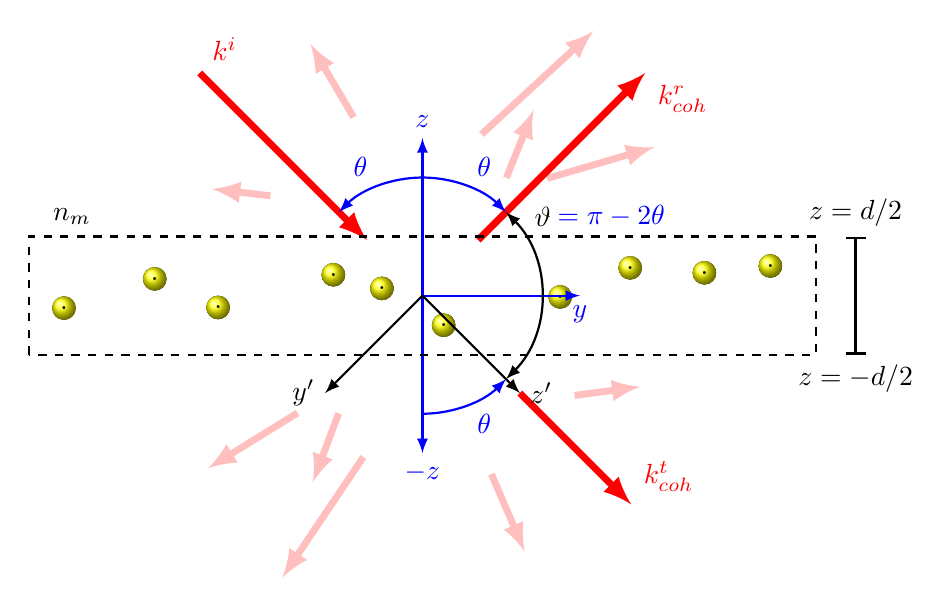
\begin{tikzpicture}[scale=1]
\def\a{.15}
\def\d{.75}
%----------------------NPs--------------
\foreach \y in {-4.5,-3.5,...,3.5,4.5}{
\fill[ball color=yellow, opacity=1] (\y+rand*.5,rand*.45) circle(\a) node[ ]{.};
}

%----------------------difussed scattered field--------------
\begin{scope}[opacity=.25, transparency group]
\foreach \s in {-1,1}{
	\draw[- latex, red, line width=2.5](0,\s*\d)++(25:\s*1.75)--(35+rand*5:\s*3.5);
	\draw[- latex, red, line width=2.5](0,\s*\d)++(35:\s*1.3)--(55+rand*5:\s*2.75);
	\draw[- latex, red, line width=2.5](0,\s*\d)++(165:\s*2)--(155+rand*5:\s*3);
	\draw[- latex, red, line width=2.5](0,\s*\d)++(120:\s*1.75)--(110+rand*5:\s*3.5);
	\draw[- latex, red, line width=2.5](0,\s*\d)++(60:\s*1.5)--(60+rand*5:\s*4);}
\end{scope}

%----------------------coherent scattered field--------------
\draw[latex -, thick, red, line width=2.5](135:1)--(135:4) node[anchor=south west]{$\vb{k}^i$};
\draw[- latex, thick, red, line width=2.5](45:1)--(45:4)node[anchor=north west]{$\vb{k}_{coh}^r$};
\draw[ - latex, thick, red, line width=2.5](-45:1.75)--(-45:3.75) node[anchor=south west]{$\vb{k}_{coh}^t$};

%----------------------Main system--------------
\draw[- latex, thick, blue] (0,0)--(90:2) node[anchor = south]{$z$};
\draw[- latex, thick, blue] (0,0)--(-90:2) node[anchor = north]{$-z$};
\draw[- latex, thick, blue] (0,0)--(0:2) node[anchor = north]{$y$};
\path (0,0)++(135/2:1.5)node[anchor=south west, blue]{$\theta$}; 
\draw[- latex, thick, blue](90:1.5)arc(90:45:1.5);
\path (0,0)++(-135/2:1.5)node[anchor=north west, blue]{$\theta$}; 
\draw[- latex, thick, blue](-90:1.5)arc(-90:-45:1.5);
\path (0,0)++(90+45/2:1.5)node[anchor=south east, blue]{$\theta$}; 
\draw[- latex, thick, blue](90:1.5)arc(90:135:1.5);

----------------------Mie system--------------
\draw[- latex, thick, black] (0,0)--(-45:1.75) node[anchor =  west]{$z'$};
\draw[- latex, thick, black] (0,0)--(-135:1.75) node[anchor =  east]{$y'$};
\path (0,0)++(30:1.5)node[anchor=south west, black]{$\vartheta$}; 
\path (0,0)++(30:1.5)node[anchor=south west, blue]{$\;\;\; =  \pi - 2\theta$}; 
\draw[latex - latex, thick, black](-45:1.5)arc(-45:45:1.5);

%----------------------thickness and slab-------------
\draw[thick, dashed] (-5,-\d) rectangle (5,\d);
%\draw[thick, dashed] (-5, 0) --  (5,0);
\draw[ |-|, thick,] (5.5,-\d) node[anchor = north]{$z=-d/2$} -- (5.5,\d) node[anchor = south]{$z=d/2$};
\node at (-4.5,1) {$\; n_m$};
\end{tikzpicture}
	\caption{Placa de grosor $d$ y volumen $V$ con $N$ partículas esféricas  idénticas, localizadas al azar e iluminadas con una onda plana monocromática con vector de onda $\vb{k}^i$. La dirección de los campos esparcidos coherentes se denotan por $\vb{k}^r_{coh}$ y $\vb{k}^t_{coh}$. Las flechas rojas sólidas representan las componentes cohrentes del campo esparcido mientras que las rosas representan la componente difusa. }\label{fig:CSM-Slab}
	\end{figure} 
 
\subsection{Monocapa suspendida en el espacio libre}
 
Para calcular los coeficientes de amplitud de reflexión y transmisión del CSM se calcula el campo eléctrico promedio esparcido por las NPs dentro de la región del espacio, caracterizado por un índice de refracción real $n_m$, delimitada por  $-d/2<z<d/2$, una placa de grosor $d$ y volumen $V$, en donde se encuentran $N$ nanopartículas esféricas idénticas, con índice de refracción $n_p$, y distribuidas espacialmente de forma aleatoria, como se observa en la Fig. \ref{fig:CSM-Slab}. Si una onda plana $\vb{E}^i = E_0 e^{i\vb{k}^i\cdot\vb{r}}\vu{e}_i$ (por simplicidad se omite la dependecia temporal), con $\vu{e}_i$ un vector en el plano de polarización de la onda plana y $|\vb{k}^i| = k = 2\pi n_m /\lambda$, incide sobre la placa, el campo eléctrico esparcido  por las NPs dentro de la placa $\vb{E}^s$ (asumiendo una densidad $N/V$ baja), puede calcularse bajo la aproximación de esparcimiento individual (Single Scattering Approximation, SSA)\index{Esparcimiento!Individual, Aproximación de (SSA)}, en donde cada NP esparce la luz sin considerar la interacción entre el campo eléctrico esparcido por las otras NPs \cite{barrera2003coherent}. Al considerar la interacción del campo eléctrico incidente con las $N$ nanopartículas dentro de la placa, el campo eléctrico esparcido por todas las partículas tiene componentes espaciales en todas las direcciones, por lo que el campo eléctrico esparcido puede descomponerse en una componente coherente y una difusa, representadas en la Fig. \ref{fig:CSM-Slab} mediante las flechas rojas y rosas, respectivamente.


El  campo eléctrico esparcido promedio $\langle \vb{E}^s\rangle$, que corresponde a la componente coherente, se calcula al considerar el promedio espacial de los campos esparcidos por las NPs dentro de la placa al suponer que la posición de una NP es independiente a la de las demás y que la probabilidad de encontrar el centro de una NP dentro del volumen de la placa es uniforme, por lo que la componente coherente del campo esparcido es  \cite{garcia2012multiple}\index{Esparcimiento!Individual, Aproximación de (SSA)!campo eléctrico esparcido promedio}
%
	\begin{align}
	\langle \vb{E}^s\rangle =
	\begin{dcases} 
	      \langle \vb{E}^s_{r,SSA}\rangle e^{i\vb{k}^r_{coh}\cdot\vb{r}} =
	    			i \frac{N}{V}  \frac{d E_0}{2} \frac{\sin(k_z^id)}{k_z^i d} 
				\frac{\mathbb{F}(\vu{k}^r,\vu{k}^i)\cdot \vu{e}_i}{k_z^i }	e^{i\vb{k}^r_{coh}\cdot\vb{r}},		& d/2<z \\
      \langle \vb{E}^s_{t,SSA}\rangle e^{i\vb{k}^t_{coh}\cdot\vb{r}} =
 				i\frac{N}{V} \frac{d E_0}{2}\frac{\mathbb{F}(\vu{k}^i,\vu{k}^i)\cdot \vu{e}_i}{k_z^i}		
				e^{i\vb{k}^t_{coh}\cdot\vb{r}},
							& z<-d/2
   \end{dcases}
   	\label{eq:AvErEt}
	\end{align}
%
en donde $k^i_z = k^i\cos\theta$; $\vb{k}^i$ es el vector de onda del campo eléctrico incidente $\vb{E}^i = \vb{E}_0 e^{i\vb{k}^i\cdot\vb{r}}$, polarizado en la dirección $\vu{e}_i$; $\vb{k}^r_{coh}$ es la dirección de propagación de la componente coherente reflejada; $\vb{k}^t_{coh}=\vb{k}^i$ es la dirección de propagación de la componente coherente transmitida; y $\mathbb{F}$ \index{Electromagnéticos!campos!operador de campo lejano} es el operador de esparcimiento de campo lejano [Ec. \eqref{eq:FarFieldDyadic}] que depende de la dirección de propagación de la onda plana incidente $\vb{k}^i$ y la del campo esparcido $\vb{k}^s$. El término $\mathbb{F}$ no limita la solución del campo eléctrico esparcido promedio al campo lejano, puesto que es un resultado derivado de promediar la respuesta EM \cite{gutierrez2012overview}.

En la Fig. \ref{fig:CSM-Slab} se observa que la dirección de propagación de  $\langle \vb{E}^s_{r,SSA}\rangle$ en $d/2<z$, dada por el vector de onda $\vb{k}^r_{coh}$ y la de $\langle \vb{E}^s_{t,SSA}\rangle$ en  $z<-d/2$, dada por $\vb{k}^t_{coh}$, forman un ángulo $\theta$ respecto a la dirección normal a la monocapa (sistema coordenado azul). A diferencia la componente difusa (flechas rosas), la componente coherente del campo eléctrico esparcido es distinta de cero al calcular el promedio espacial, ya que los campos eléctricos esparcidos por cada NP en la placa interfieren constructivamente en las direcciones de esparcimiento $\vu{k}^s =\vu{k}^i=\vu{k}^t_{coh}$ y $\vu{k}^s =\vu{k}^r_{coh}$ \cite{garcia2012multiple}. Puesto que las NPs dentro de la placa son esféricas e idénticas, se calcula la expresión del operador de esparcimiento $\mathbb{F}(\vu{k}^s,\vu{k}^i)$ al comparar su expresión general [Ec. \eqref{eq:FarFieldDyadic}] con la matriz de esparcimiento de Mie [Ec. \eqref{eq:MieMatrix}]\index{Mie!matriz de esparcimiento de}, por lo que el operador de esparcimiento de campo lejano es
%
	\begin{align}
	\mathbb{F}(\vu{k}^s,\vu{k}^i) = \frac{1}{-ik} 
	 \mqty(S_2(\vartheta) & 0 \\ 0 & S_1(\vartheta)),
	 \label{eq:FFDydadic-Mie}
	\end{align}
%
en donde $\vartheta$ denota el ángulo entre la dirección del campo esparcido $\vu{k}^s$ y del campo incidente $\vu{k}^i$, con $\vartheta = 0$ para $\vu{k}^s = \vu{k}^t_{coh}$ y $\vartheta = \pi-2\theta$  para $\vu{k}^s = \vu{k}^r_{coh}$, como se observa en la Fig. \ref{fig:CSM-Slab}.
	
Al sustituir la Ec. \eqref{eq:FFDydadic-Mie} en la Ec. \eqref{eq:AvErEt} y multiplicar las expresiones resultantes por $(3ka^3)/(3ka^3)$, con $a$ el radio de las NPs y $k = 2\pi n_m /\lambda$, y agrupar términos, se obtienen las siguientes expresiones 
%
	\begin{subequations}\begin{align}
		\langle \vb{E}^s_{r,SSA}\rangle & = - \frac{E_0}{\cos\theta_i} \frac32  \qty(\frac{N}{V} \frac43\pi a^3)\frac{kd}{(ka)^3}   \frac{\sin(k_z^id)}{k_z^i d}  S_j(\vartheta)\vu{e}_i =
		-\alpha  \frac{\sin(k_z^id)}{k_z^i d}   S_j(\vartheta) \vb{E}_0,
		\label{eqs:EsSSAr}\\
	\langle \vb{E}^s_{t,SSA}\rangle &=  - \frac{E_0}{\cos\theta_i} \frac32
						 \qty(\frac{N}{V}\frac43\pi a^3  ) \frac{kd}{(ka)^3}  S_j(0) \vu{e}_i  
						 = - \alpha S(0) \vb{E}_0,
		\label{eqs:EsSSAt}
	\end{align}\label{eq:EsSSA}\end{subequations}
%
donde  se emplea $j=1$ para polarización $s$ y $j=2$ para $p$ en los elementos de matriz no nulos de la matriz de esparcimiento de Mie, $S_j(\vartheta)$, y donde se define $S(0) \equiv S_1(0)=S_2(0)$\index{Mie!matriz de esparcimiento de!elementos de la [$S_j(\theta)$]}\index{Esparcimiento!de Mie, matriz de}. La expresión de $\alpha$ en las Ecs. \eqref{eq:EsSSA} en términos del parámetro de tamaño $x=ka$ es
%
\begin{align*}
	\alpha \equiv \frac32 \qty(\frac{N}{V}\frac43 \pi a^3  )\frac{kd}{x^3\cos\theta_i} = \frac32\frac{kd}{ x^3\cos\theta_i} f,
	\end{align*}
%
con $f= N 4\pi a^3/(3V)$ la fracción volumétrica de llenado, que es el cociente entre el volumen que ocupan todas las NPs de la placa entre el volumen de ésta. Si se considera el límite $d\to 0$, lo que equivale a tener una monocapa de partículas esféricas desordenadas y al asumir que la componente difusa del campo esparcido por las partículas es despreciable en comparación a la componente coherente, es posible definir los coeficientes de amplitud de reflexión y transimisión en la SSA a partir de las Ecs. \eqref{eq:EsSSA} como\index{Esparcimiento!Individual, Aproximación de (SSA)!coeficientes de amplitud}
	
	\begin{subequations}\eqhalf{r_{coh}^{SSA} = -\alpha S_j(\vartheta),}
	\eqhalf{t_{coh}^{SSA} = 1 - \alpha S(0), }
	\label{eqs:rtcohSSA}\end{subequations}\vspace*{-1em}	
	
\noindent considerando para el coeficiente de amplitud de transmisión la contribución de la onda plana incidente en la Ec. \eqref{eqs:EsSSAt}, y al considerar que $V = A d$, con $A$ el área de la monocapa paralela al plano $z=0$, el coeficiente $\alpha$ se reescribe como
%
	\begin{align}
	\alpha = \frac{2\Theta}{x^2 \cos\theta_i},
	\label{eq:alpha}
	\end{align}
%
donde $\Theta = N \pi a^2 / A$ es la fracción de cubierta, que corresponde al área proyectada por todas las esferas sobre el área de la placa. La distancia mínima promedio $\langle\mathscr{D}_{min}\rangle$ entre las NPs de una monocapa se relaciona con su fracción de cubierta $\Theta$ mediante la expresión $\Theta = \pi a^2 / (2a+\langle\mathscr{D}_{min}\rangle)^2$, como se observa en la Fig. \ref{fig:MeanD}. Entonces, la separación mínima promedio entre las NPs de la monocapa es
%
	\begin{equation}
	\frac{\langle\mathscr{D}_{min}\rangle}{a} = \sqrt{\frac{\pi}{\Theta}}-2,
	\label{eq:MeanD}
	\end{equation}
%
de donde se deduce que el valor máximo de $\Theta$ es $0.78$, cuando $\langle\mathscr{D}_{min}\rangle=0$, y que cuando $\langle\mathscr{D}_{min}\rangle= a$ se cumple que $\Theta = \pi/9\approx 0.349$. El cociente entre la distancia mínima promedio entre NPs y su radio se calcula para algunos valores en la Tabla  \ref{tab:meanD}.

\begin{table}[h!] \centering
	\caption{Cociente entre la distancia promedio $\langle\mathscr{D}_{min}\rangle$ entre NPs y su radio $a$, para una monocapa de NPs esféricas e idénticas con fracción de cubierta $\Theta$.}
	\label{tab:meanD}\vspace*{-1em}
	\begin{tabular}{c || c c c c c c c c}
	\hline \hline
	$\Theta$ & $0.05$ & $0.1$ & $0.2$ & $0.3$ & $0.4$ & $0.5$ & $0.6$ & $0.7$\\
 \hline 
	$\langle\mathscr{D}_{min}\rangle / a $& $5.93$ & $3.60$ & $1.96$ & $1.23$ & $0.80$ & $0.51$ & $0.29$ & $0.12$ \\
	\hline \hline
	\end{tabular} 
\end{table}

\begin{figure}[h!]\centering
		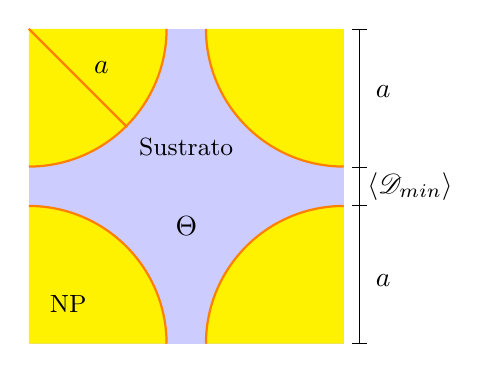
\begin{tikzpicture}[scale=1]
\def	\ll{2}
\def\a{1.75}
%------------------------------------------------ NPs and Substrate
\fill[blue!20] (-\ll,-\ll) rectangle (\ll,\ll);		

\fill[-,yellow,shift ={(-\ll,-\ll)}, opacity = 1](90:\a)arc(90:0:\a)--(0,0)--(90:\a);
\draw[-, orange, thick, shift ={(-\ll,-\ll)}](90:\a)arc(90:0:\a);

\fill[-,yellow,shift ={(-\ll,\ll)}, opacity = 1](-90:\a)arc(-90:0:\a)--(0,0)--(-90:\a);
\draw[-, orange, thick, shift ={(-\ll,\ll)}](-90:\a)arc(-90:0:\a);

\fill[-,yellow,shift ={(\ll,\ll)}, opacity = 1](-90:\a)arc(-90:-180:\a)--(0,0)--(-90:\a);
\draw[-, orange, thick, shift ={(\ll,\ll)}](-90:\a)arc(-90:-180:\a);

\fill[-,yellow,shift ={(\ll,-\ll)}, opacity = 1](90:\a)arc(90:180:\a)--(0,0)--(90:\a);
\draw[-, orange, thick, shift ={(\ll,-\ll)}](90:\a)arc(90:180:\a);

\draw[-, thick, orange] (-\ll,\ll)--(-\ll*.65,\ll*.65) node [anchor = south west]{\color{black}$a$}--(-.75,.75);
%-------------------------------------------------- media names
\node at (0,.5) {\small Sustrato}; 
\node at (-1.5,-1.5) {\small NP};
\node at (0,-.5) {$\Theta$};

%--------------------------------------------------- dimensions
\draw[-|] (\ll+.2,\ll-\a)--(\ll+.2,\ll);
\node at (\ll+.5, \ll*.6){$a$};

\draw[-|] (\ll+.2,-\ll+\a)--(\ll+.2,-\ll);
\node at (\ll+.5,-\ll*.6){$a$};

\draw[|-|] (\ll+.2,\ll-\a)--(\ll+.2,-\ll+\a);
\node at (\ll+.5, 0){$\;\;\;\;\;\;\;\langle\mathscr{D}_{min}\rangle $};

\end{tikzpicture}
		\caption{ Vista superior de una monocapa de NPs de radio $a$ con fracción de cubierta $\Theta$ sobre un sustrato. La separación promedio entre las NPs es $\langle\mathscr{D}_{min}\rangle $, por lo que el área total del cuadrado es $(2a+\langle d \rangle)^2$, el de una NP es $\pi a^2$ y por tanto $\Theta= \pi a^2 / (2a+\langle\mathscr{D}_{min}\rangle )^2$.}\label{fig:MeanD}
	\end{figure}	
	
Al analizar  las Ecs. \eqref{eqs:rtcohSSA} y \eqref{eq:alpha} para ángulos rasantes $\theta\to \pi/2$, se observa que $\alpha\to \infty$, además de que para partículas pequeñas $x\ll 1$ el producto $r_{coh}^{SSA}r_{coh}^{SSA*}$ puede tomar valores mayores a la unidad. Por tanto, los coeficientes de amplitud calculados a partir de la SSA son válidos únicamente para ángulos de incidencia no rasantes  \cite{reyes2018analytical}.

Para calcular los coeficientes de amplitud de reflexión y transmisión para una monocapa de NPs que no estén limitados a ángulos de incidencia bajos, se deben considerar contribuciones de esparcimiento múltiple (Multiple Scattering, MS)\index{Esparcimiento!Múltiple (MS)!campo eléctrico esparcido promedio} en el cálculo del campo eléctrico $\vb{E}^{exc}$  que excita a las partículas dentro de la placa, el cual se puede descomponer como 
	\begin{align}
	\vb{E}^{exc} = \vb{E}^{exc}_{t} e^{i\vb{k}^t_{coh}\cdot\vb{r}}+
					\vb{E}^{exc}_{r} e^{i\vb{k}^r_{coh}\cdot\vb{r}},
	\end{align}
donde  $\vb{E}^{exc}_t$ es la componente del campo eléctrico que excita a las NPs que se transmite según la SSA y $\vb{E}^{exc}_{r}$ la que se refleja; dado que la reflexión y transmisión de $\vb{E}^{exc}$ están dadas por las Ecs. \eqref{eq:EsSSA}, su polarización es la de la onda plana $\vu{e}_i$ y su dirección de propagación está dada por $\vb{k}^t_{coh}$ y $\vb{k}^r_{coh}$, respectivamente. Entonces, el campo eléctrico esparcido promedio considerando el MS $\vb{E}^s_{MS}$, toma en cuenta  las reflexiones y transmisiones de $\vb{E}^{exc}$ según las Ecs. \eqref{eq:EsSSA} en el límite $d\to 0$ \cite{gutierrez2012overview}, como se observa en la Fig. \ref{fig:MScatt-slab-MS}, y la contribución del campo eléctrico incidente $\vb{E}^i$, por lo que  \cite{reyes2018analytical}
%
	\begin{subequations}\begin{align}
		\langle \vb{E}^s_{r,coh}\rangle & =	\langle \vb{E}^s_{r,\textit{MS}}\rangle
					= \qty[-\alpha S_j(\vartheta)E^{exc}_t -\alpha S(0)E^{exc}_r
					]\vu{e}_i e^{i\vb{k}^r_{coh}\cdot\vb{r}},\\
		\langle \vb{E}^s_{t,coh}\rangle & =\vb{E}^i+\langle\vb{E}^s_{t,\textit{MS}}\rangle
					= \qty[E_0 -\alpha S(0)E^{exc}_t 
					-\alpha	 S_j(\vartheta)E^{exc}_r
					]\vu{e}_i e^{i\vb{k}^t_{coh}\cdot\vb{r}}.
	\end{align} \label{eqs:EsMS}\end{subequations} \vspace*{-2em}

	\begin{figure}[h!]\centering
		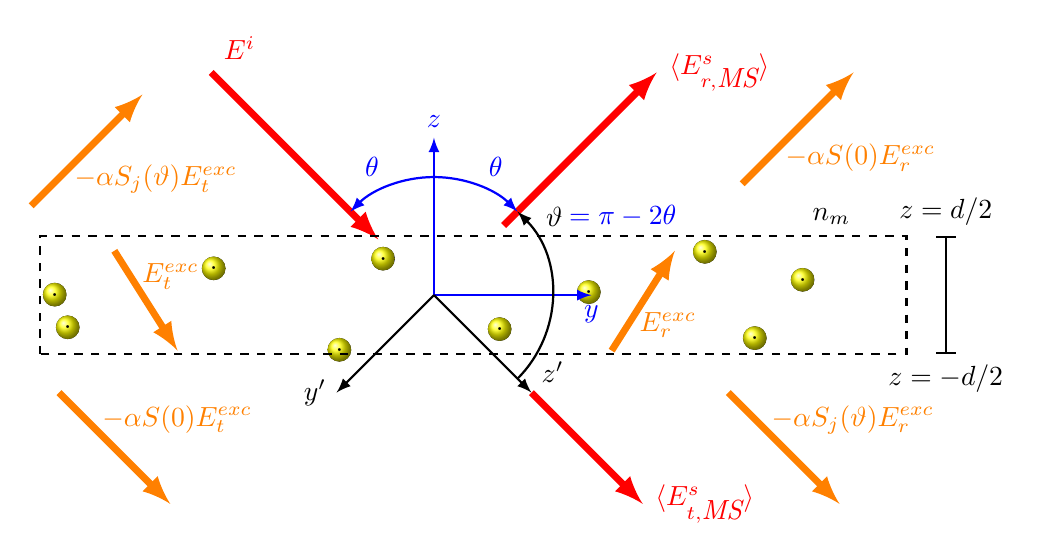
\begin{tikzpicture}[scale=1]
\def\a{.15}
\def\d{.75}

%----------------------NPs--------------
\foreach \y in {-4.5,-4.5,-2.5,-1.5,-.5,.5,1.5,3.5,4,4.5}{
\fill[ball color=yellow, opacity=1] (\y+rand*.5,rand*\d) circle(\a) node[ ]{.};
}

%----------------------averaged fields ---------------------
\draw[latex -, thick, red, line width=2.5](135:1)--(135:4) node[anchor=south west]{$\vb{E}^i$};
\draw[- latex, thick, red, line width=2.5](45:\d+.5)--(45:4)node[anchor=west]{$\langle\vb{E}_{r,\textit{MS}}^s\rangle$};
\draw[ - latex, thick, red, line width=2.5](-45:1.75)--(-45:3.75) node[anchor=west]{$\langle\vb{E}_{t,\textit{MS}}^s\rangle$};

%---------------------- Exciting fields ---------------------
\draw[- latex , thick,  orange, line width=2.5,shift ={(-3,0)}](152:1.2)node[anchor= north west]{$\;\;\vb{E}^{exc}_t$}--(250:\d);
\draw[latex - , thick, orange, line width=2.5,shift ={(2,0)}](28:1.2)--(-70:\d) node[anchor= south west]{$\;\;\vb{E}^{exc}_r$};

%-------------- reflected and transmitted exciting fields DOWN ---------------------
\draw[latex - , thick, orange, line width=2.5,shift={(2.5, 0)}](-45:3.75)--(-45:1.75) node[anchor=north west]{$\;\;\;\;-\alpha S_j(\vartheta)\vb{E}^{exc}_r$};
\draw[latex - , thick, orange, line width=2.5,shift={(-6, 0)}](-45:3.75)--(-45:1.75) node[anchor=north west]{$\;\;\;\;-\alpha S(0)\vb{E}^{exc}_t$};

%-------------reflected and transmitted exciting fields UP ---------------------
\draw[latex -, thick, orange, line width=2.5,shift={(2.5, 0)}](45:4)--(45:2)node[anchor=south west]{$\;\;\;\;-\alpha S(0) \vb{E}^{exc}_r$};
\draw[latex -, thick, orange, line width=2.5,shift={(-6, .25)}](45:3.25)--(45:\d+.5)node[anchor=south west]{$\;\;\;\;-\alpha S_j(\vartheta) \vb{E}^{exc}_t$};

%----------------------main system---------------------
\draw[- latex, thick, blue] (0,0)--(90:2) node[anchor = south]{$z$};
\draw[- latex, thick, blue] (0,0)--(0:2) node[anchor = north]{$y$};
\path (0,0)++(135/2:1.5)node[anchor=south west, blue]{$\theta$}; 
\draw[- latex, thick, blue](90:1.5)arc(90:45:1.5);
\path (0,0)++(90+45/2:1.5)node[anchor=south east, blue]{$\theta$}; 
\draw[- latex, thick, blue](90:1.5)arc(90:135:1.5);

%----------------------Mie system---------------------
\draw[- latex, thick, black] (0,0)--(-45:1.75) node[anchor = south west]{$z'$};
\draw[- latex, thick, black] (0,0)--(-135:1.75) node[anchor = east]{$y'$};
\path (0,0)++(30:1.5)node[anchor=south west, black]{$\vartheta$}; 
\path (0,0)++(30:1.5)node[anchor=south west, blue]{$\;\;\; =  \pi - 2\theta$}; 
\draw[- latex, thick, black](-45:1.5)arc(-45:45:1.5);

%----------------------thickness and slab ---------------------
\draw[thick, dashed] (-5,-\d) rectangle (6,\d);
%\draw[thick, dashed] (-5, 0) --  (6,0);
\draw[ |-|, thick,] (6.5,-\d) node[anchor = north]{$z=-d/2$} -- (6.5,\d) node[anchor = south]{$z=d/2$};
\node at (5,1) {$\; n_m$};
\end{tikzpicture}
		\caption{ Película de grosor $d$ y volumen $V$ con $N$ partículas esféricas idénticas excitada por una onda plana monocromática incidente en la dirección $\vb{k}^i$. El campo eléctrico que excita a las NPs dentro de la película $\vb{E}^{exc}$ se divide en una componente reflejada $ \vb{E}^{exc}_r$ y una transmitida $ \vb{E}^{exc}_t$, considerando así el esparcimiento múltiple por las NPs. Los campos eléctricos esparcidos promedio reflejado $\langle \vb{E}^s_{r,coh}\rangle$ y transmitido $\langle \vb{E}^s_{r,coh}\rangle$ corresponden a la suma  de las Ecs. \eqref{eqs:rtcohSSA} aplicadas a $\vb{E}^{exc}_t$ y a $\vb{E}^{exc}_r$ como se representa en la figura y en las Ecs. \eqref{eqs:EsMS}. Las flechas rojas corresponden a la onda plana incidente y los campos esparcidos promedios mientras que las flechas naranjas corresponden al campo que excita a las NPs. }\label{fig:MScatt-slab-MS}
	\end{figure}	
	
Para determinar la expresión del campo eléctrico que excita a las NPs en la placa $\vb{E}^{exc}$ considerando el MS\footnote{El procedimiento descrito emplea un enfoque heurístico que se publicó en \cite{reyes2018analytical} sin emabargo, un enfoque más riguroso se encuentra en \cite{barrera2003coherent}.}, se divide la placa donde se encuentran las NPs en dos (de grosor $d/2$ cada una) y se calcula el promedio de  $\vb{E}^{exc}$ en la interfaz entre las dos placas ($z=0$) de forma autoconsistente, por lo que las NPs en la placa no sólo son iluminadas por el campo eléctrico incidente $\vb{E}^i$, sino también por $\vb{E}^{exc}$ \cite{reyes2018analytical}. El campo $\vb{E}^{exc}$ se puede descomponer en una componente transmitida $\vb{E}^{exc}_{t}$ y una reflejada, $\vb{E}^{exc}_{t}$. Para calcular $\vb{E}^{exc}_{t}$ de forma autoconsistente se considera que $\vb{E}^{exc}_{t}$ es igual a la suma del campo eléctrico incidente más el promedio de la transmisión del campo $E^{exc}_t$ y a la reflexión del campo $E^{exc}_r$ ---que corresponden a la suma de los campos esparcidos por las NPs en la placa superior ($0<z<d/2$)--- , es decir,
%
	\begin{subequations}\begin{align}
		\vb{E}^{exc}_t  e^{i\vb{k}^i\cdot\vb{r}}  =
				\qty[E_0  - \frac12 \qty(
					\alpha S(0)E^{exc}_t + \alpha S_j(\vartheta)E^{exc}_r
				)] e^{i\vb{k}^t_{coh}\cdot\vb{r}}  \vu{e}_i,
	\end{align}
%
donde el factor $1/2$ indica que es la respuesta EM promedio dentro de la placa. Asimismo, el campo $\vb{E}^{exc}_{r}$ se calcula de forma autoconsistente como la reflexión  del campo $E^{exc}_t$ y la transmisión del campo $E^{exc}_r$ ---campos esparcidos por las NPs en la placa inferior ($-d/2<z<0$)---, por lo que su expresión es	
%
	\begin{align}
	\vb{E}^{exc}_r  e^{i\vb{k}^r\cdot\vb{r}}  =
				\qty[- \frac12 \qty(
					\alpha S_j(\vartheta)E^{exc}_t + \alpha S(0)E^{exc}_r
				)] e^{i\vb{k}^r_{coh}\cdot\vb{r}}  \vu{e}_i.
	\end{align} \label{eq:Eexc}\end{subequations}
%
En la Fig. \ref{fig:Eexc} se muestra una representación gráfica de las Ecs. \eqref{eq:Eexc}, que son válidas únicamente en $-d/2<z<d/2$.

\begin{figure}[h!]\centering
	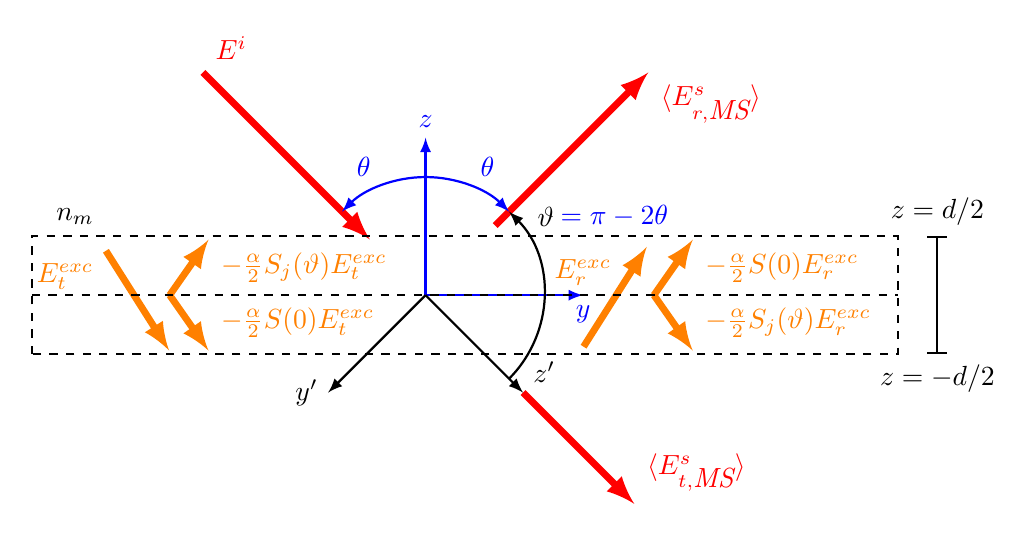
\begin{tikzpicture}[scale=1]
\def\a{.15}
\def\d{.75}

%\foreach \y in {-4.5,-3.5,-2.5,-.5,.5,2.5,3.5,4.5}{
%\fill[ball color=yellow, opacity=1] (\y+rand*.5,rand*\d) circle(\a) node[ ]{.};
%}


\draw[latex -, thick, red, line width=2.5](135:1)--(135:4) node[anchor=south west]{$\vb{E}^i$};
\draw[- latex, thick, red, line width=2.5](45:\d+.5)--(45:4)node[anchor=north west]{$\langle\vb{E}_{r,\textit{MS}}^s\rangle$};
\draw[ - latex, thick, red, line width=2.5](-45:1.75)--(-45:3.75) node[anchor=south west]{$\langle\vb{E}_{t,\textit{MS}}^s\rangle$};

%---------------------- Exciting transmitted field ---------------------
\draw[latex - , thick,  orange, line width=2.5,shift={(-3., 0)}](250:\d)--(152:1.2) node[anchor= north east]{$\vb{E}^{exc}_t$};

\draw[- latex , thick,  orange, line width=2.5, shift={(-2.5, 0)}](180:\d)--(250:\d) node[anchor= south west]{$-\frac{\alpha}{2} S(0)\vb{E}^{exc}_t$};
\draw[- latex , thick,  orange, line width=2.5, shift={(-2.5, 0)}](180:\d)--(110:\d) node[anchor= north west]{$-\frac{\alpha}{2} S_j(\vartheta)\vb{E}^{exc}_t$};

%---------------------- Exciting reflected field ---------------------
\draw[- latex , thick, orange, line width=2.5,shift={(1.75, .05)}](-70:\d)--(28:1.2) node[anchor=north east]{$\vb{E}^{exc}_r\;\;\;$};

\draw[- latex , thick,  orange, line width=2.5, shift={(3.65, 0)}](180:\d)--(250:\d) node[anchor= south west]{$-\frac{\alpha}{2} S_j(\vartheta)\vb{E}^{exc}_r$};
\draw[- latex , thick,  orange, line width=2.5, shift={(3.65, 0)}](180:\d)--(110:\d) node[anchor= north west]{$-\frac{\alpha}{2}S(0)\vb{E}^{exc}_r$};

%----------------------Main system---------------------
\draw[- latex, thick, blue] (0,0)--(90:2) node[anchor = south]{$z$};
\draw[- latex, thick, blue] (0,0)--(0:2) node[anchor = north]{$y$};
\path (0,0)++(135/2:1.5)node[anchor=south west, blue]{$\theta$}; 
\draw[- latex, thick, blue](90:1.5)arc(90:45:1.5);
\path (0,0)++(90+45/2:1.5)node[anchor=south east, blue]{$\theta$}; 
\draw[- latex, thick, blue](90:1.5)arc(90:135:1.5);

%----------------------Mie system---------------------
\draw[- latex, thick, black] (0,0)--(-45:1.75) node[anchor = south west]{$z'$};
\draw[- latex, thick, black] (0,0)--(-135:1.75) node[anchor = east]{$y'$};
\path (0,0)++(30:1.5)node[anchor=south west, black]{$\vartheta$}; 
\path (0,0)++(30:1.5)node[anchor=south west, blue]{$\;\;\; =  \pi - 2\theta$}; 
\draw[- latex, thick, black](-45:1.5)arc(-45:45:1.5);

%----------------------thickness and slab ---------------------
\draw[thick, dashed] (-5,-\d) rectangle (6,\d);
\draw[thick, dashed] (-5, 0) --  (6,0);
\draw[ |-|, thick,] (6.5,-\d) node[anchor = north]{$z=-d/2$} -- (6.5,\d) node[anchor = south]{$z=d/2$};
\node at (-4.5,1) {$\; n_m$};

\end{tikzpicture}
	\caption{ Película de grosor $d$ y volumen $V$ con $N$ partículas esféricas idénticas (no mostradas en la figura) dividida en dos regiones: $z<0$ y $z>0$. Una onda plana monocromática propagándose en la dirección $\vb{k}^i$ incide en las placas, generando un campo eléctrico que excita a las NPs dentro de la película y que considera el esparcimiento múltiple de las NPs al dividirlo en una componente reflejada $\vb{E}^{exc}_r$ y una transmitida $\vb{E}^{exc}_t$, dando como resultado los campos esparcidos promedio reflejado $\langle\vb{E}_{r,\textit{MS}}^s\rangle$ y transmitido $\langle\vb{E}_{t,\textit{MS}}^s\rangle$. Sobre la interfaz entre las dos placas ($z=0$) tanto $\vb{E}^{exc}_r$ como $\vb{E}^{exc}_t$ se reflejan y transmiten según las Ecs. \eqref{eqs:rtcohSSA}, proceso descrito por las Ecs. \eqref{eq:Eexc}. Las flechas rojas corresponden a la onda plana incidente y los campos esparcidos promedios, mientras que las flechas naranjas corresponden al campo que excita a las NPs. }\label{fig:Eexc}
	\end{figure}	
	
Al resolver las Ecs. \eqref{eq:Eexc} para $E^{exc}_t$ y $E^{exc}_r$ en términos del campo eléctrico incidente $\vb{E}_0$ se obtienen las siguientes expresiones
%
	\begin{align*}
	\vb{E}^{exc}_t  &= \frac{1+\frac12\alpha S(0)}
				{1+\alpha S(0) +\frac14\alpha^2\qty[S^2(0)-S_j^2(\vartheta)]}\vb{E}_0,\\
	\vb{E}^{exc}_r  &= \frac{-\frac12\alpha S_j(\vartheta)}
				{1+\alpha S(0) +\frac14\alpha^2\qty[S^2(0)-S_j^2(\vartheta)]}\vb{E}_0,
	\end{align*}
%
por lo que, al sustituirlas en las expresiones de los campos esparcidos promedio reflejados y transmitidos [Ecs. \eqref{eqs:EsMS}], se obtienen
%
	\begin{align*}
	\langle \vb{E}^s_{r,coh}\rangle &=
			\frac{-\alpha S_j(\vartheta)}{1+\alpha S(0)+\frac14 \alpha^2 \left[S^2(0)-S_j^2 (\vartheta) \right]} \vb{E}_0 e^{i\vb{k}^r_{coh}\cdot\vb{r}},\\
	\langle \vb{E}^s_{r,coh}\rangle &=
			\frac{1-\frac14\alpha^2\qty[S^2(0)-S_j^2(\vartheta)]}{1+\alpha S(0)+\frac14 \alpha^2 \left[S^2(0)-S_j^2 (\vartheta) \right]} \vb{E}_0 e^{i\vb{k}^t_{coh}\cdot\vb{r}},
	\end{align*}
%
de donde es posible calcular los coeficientes de amplitud de reflexión y transmisión para una monocapa de NPs esféricas bajo el formalismo del CSM. Entonces, considerando que el campo eléctrico que excita a las NPs toma en cuenta el esparcimiento múltiple y que la componente coherente del campo esparcido es mucho mayor que la contribución de la componente difusa, así como $\vartheta = \pi-2\theta$, se obtiene que\index{Esparcimiento!Coherente, Modelo de (CSM)!coeficientes de amplitud! para una monocapa en espacio libre} \vspace*{-.75em}
%
	\begin{subequations}\begin{tcolorbox}[title = Coeficientes de amplitud del CSM, breakable ]
	\begin{align}
	r_{coh}&=\frac{-\alpha S_j(\pi-2\theta)}
				{1+\alpha S(0)+\frac14 \alpha^2 \left[S^2(0)-S_j^2 (\pi-2\theta) \right]},
			\label{seq:rcoh}\\
	t_{coh}&=\frac{1-\frac14\alpha^2\qty[S^2(0)-S_j^2(\pi-2\theta)]}
				{1+\alpha S(0)+\frac14 \alpha^2 \left[S^2(0)-S_j^2 (\pi-2\theta) \right]},
		\label{seq:tcoh}
	\end{align}
	con $j=1$ para polarización $s$, $j=2$ para $p$ y $S(0)=S_1(0)=S_2(0)$.
	\end{tcolorbox}\label{eqs:rtcoh}\end{subequations}\vspace*{-.75em}\noindent

	 \subsection{Monocapa soportada sobre un sustrato}

Las Ecs. \eqref{eqs:rtcoh} corresponden a los coeficientes de amplitud de reflexión y transmisión de una onda plana $\vb{E}^i$ que incide a un ángulo $\theta$ sobre una monocapa de NPs esféricas, idénticas, de radio $a$ e índice de refracción $n_p$, localizadas de forma aleatoria e inmersa en una matriz con índice de refracción $n_m$, sin ser soportada de alguna forma. Sin embargo, en la realidad las NPs no pueden estar embebida en un espacio libre, sino que están soportadas sobre un sustrato, de índice de refracción $n_s$; adicionalmente la incidencia del haz de luz puede ser tanto en configuración externa, como se muestra en la Fig. \ref{figs:CSM-Ext}, como en interna, es decir ATR, como se muestra en la Fig. \ref{figs:CSM-ATR}.

	\begin{figure}[h!]\centering
	\begin{subfigure}{.05\textwidth}\vspace{-4.5cm}\caption{}\label{figs:CSM-Ext}\end{subfigure}\hspace*{-2em}
	\begin{subfigure}{.48\textwidth}
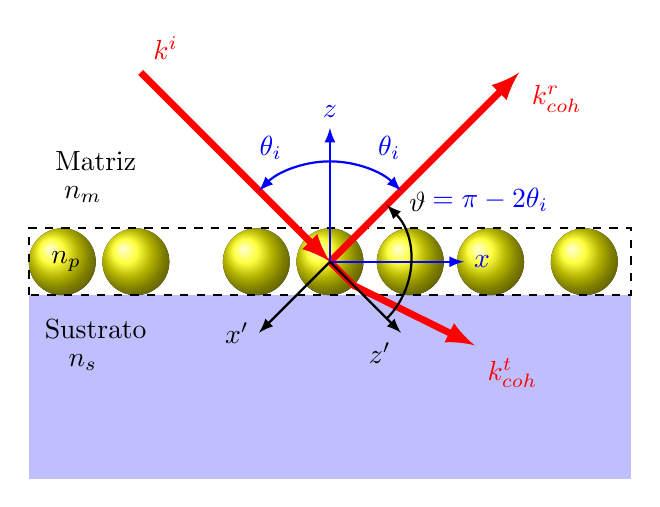
\begin{tikzpicture}[scale=.85]
\def\a{. 5}
\def\d{. 5}

\fill[blue, opacity=. 25] (-4. 5,-6.5*\d) rectangle (4. 5,-\d);

\foreach \x in {-4,-2. 9,-1. 1,0,1. 2,2. 4,3. 8}{
\fill[ball color=yellow, opacity=1] (\x,0) circle(\a);}


\draw[thick, dashed] (-4. 5,-\d) rectangle (4. 5,\d);

\draw[latex -, thick, red, line width=2. 5](135:0)--(135:4) node[anchor=south west]{$\vb{k}^i$};
\draw[- latex, thick, red, line width=2. 5](135:0)--(135:-.5)--(150:-2.5) node[anchor=north west]{$\vb{k}^t_{coh}$};
\draw[- latex, thick, red, line width=2. 5](45:0)--(45:4)node[anchor=north west]{$\vb{k}^r_{coh}$};

\draw[- latex, thick, blue] (0,0)--(90:2) node[anchor = south]{$z$};
\draw[- latex, thick, blue] (0,0)--(0:2) node[anchor = west]{$x$};
\path (0,0)++(135/2:1. 5)node[anchor=south west, blue]{$\theta_i$}; 
\draw[- latex, thick, blue](90:1. 5)arc(90:45:1. 5);
\path (0,0)++(90+45/2:1. 5)node[anchor=south east, blue]{$\theta_i$}; 
\draw[- latex, thick, blue](90:1. 5)arc(90:135:1. 5);

\draw[- latex, thick, black] (0,0)--(-45:1. 5) node[anchor = north east]{$z'$};
\draw[- latex, thick, black] (0,0)--(-135:1. 5) node[anchor = east]{$x'$};
\path (0,0)++(30:1. 2)node[anchor=south west, black]{$\vartheta$}; 
\path (0,0)++(30:1. 2)node[anchor=south west, blue]{$\;\;\; =  \pi - 2\theta_i$}; 
\draw[- latex, thick, black](-45:1. 2)arc(-45:45:1. 2);



\node at (-3.5,1.5) {Matriz};
\node at (-3.75,1) {$\; n_m$};
\node at (-4,0) {$\; n_p$};
\node at (-3.75,-1.5) {$\; n_s$};
\node at (-3.5,-1) {Sustrato};	
\end{tikzpicture}
	\end{subfigure}
	\begin{subfigure}{.05\textwidth}\vspace{-4.5cm}\caption{}\label{figs:CSM-ATR}	\end{subfigure}\hspace*{-2em}
	\begin{subfigure}{.48\textwidth} 
		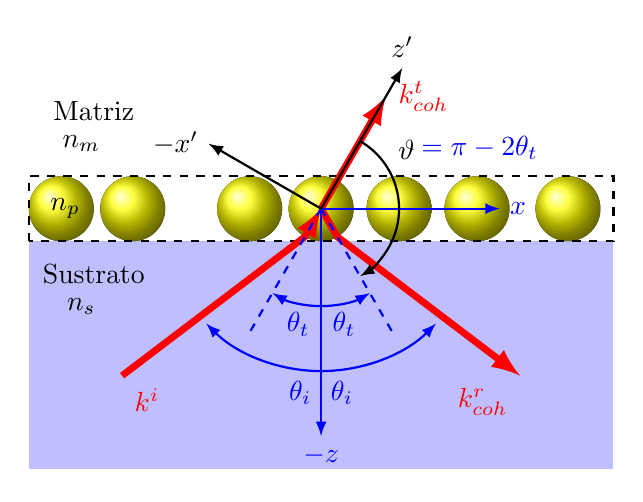
\begin{tikzpicture}[scale=.825]
\def\a{. 5}
\def\d{. 5}

\fill[blue, opacity=. 25] (-4. 5,-8*\d) rectangle (4. 5,-\d);

\foreach \x in {-4,-2. 9,-1. 1,0,1. 2,2. 4,3. 8}{
\fill[ball color=yellow, opacity=1] (\x,0) circle(\a);}


\draw[thick, dashed] (-4. 5,-\d) rectangle (4. 5,\d);

\draw[latex -, thick, red, line width=2. 5](0,0)--(-120:. 5)--(-140:4) node[anchor=north west]{$\vb{k}^i$};
\draw[- latex, thick, red, line width=2. 5](0,0)--(-120:-2)node[anchor=west]{$\vb{k}^t_{coh}$};
\draw[- latex, thick, red, line width=2. 5](0,0)--(-60:. 5)--(-40:4)node[anchor=north east]{$\vb{k}^r_{coh}$};

\draw[- latex, thick, blue] (0,0)--(-90:3. 5) node[anchor = north]{$-z$};
\draw[- latex, thick, blue] (0,0)--(0:2. 75) node[anchor = west]{$x$};

\path (0,0)++(-90:2. 5)node[anchor=north east, blue]{$\theta_i$}; 
\draw[- latex, thick, blue](-90:2. 5)arc(-90:-45:2. 5);
\path (0,0)++(-90:2. 5)node[anchor=north west, blue]{$\theta_i$}; 
\draw[- latex, thick, blue](-90:2. 5)arc(-90:-135:2. 5);

\draw[thick, blue, dashed](0,0) -- (-120:2. 25);
\draw[thick, blue, dashed](0,0) -- (-60:2. 25);
\path (0,0)++(-90-50/2:1. 6)node[anchor=north west, blue]{$\theta_t$}; 
\draw[- latex, thick, blue](-90:1. 5)arc(-90:-60:1. 5);
\path (0,0)++(-90+50/2:1. 6)node[anchor=north east, blue]{$\theta_t$}; 
\draw[- latex, thick, blue](-90:1. 5)arc(-90:-120:1. 5);

\draw[- latex, thick, black] (0,0)--(60:2.5) node[anchor = south]{$z'$};
\draw[- latex, thick, black] (0,0)--(150:2) node[anchor =  east]{$-x'$};
\path (0,0)++(30:1. 2)node[anchor=south west, black]{$\vartheta$}; 
\path (0,0)++(30:1. 2)node[anchor=south west, blue]{$\;\;\; =  \pi - 2\theta_t$}; 
\draw[- latex, thick, black](60:1. 2)arc(60:-60:1. 2);


\node at (-3.5,1.5) {Matriz};
\node at (-3.75,1) {$\; n_m$};
\node at (-4,0) {$\; n_p$};
\node at (-3.75,-1.5) {$\; n_s$};
\node at (-3.5,-1) {Sustrato};	
\end{tikzpicture}
	\vspace*{-.35em}\end{subfigure}
	\caption{Esquema de la reflexión coherente de una monocapa de NPs esféricas, con índice de refracción $n_p$,  suspendida en una matriz con índice de refracción $n_m$ y soportada por un sustrato con índice de refracción $n_s$, iluminada en un esquema de \textbf{a)} incidencia externa  y \textbf{b)} en configuración ATR. El sistema coordenado azul, con el eje $z$ paralelo a la dirección normal a la monocapa, define los ángulos de incidencia $\theta_i$, de reflexión y de transmisión $\theta_t$ mediante la ley de la reflexión y la ley de Snell. El sistema coordenado negro, con el eje $z$ paralelo a $\vb{k}^i$ en \textbf{a)} y paralelo a $\vb{k}^t_{coh}$ en \textbf{b)}, se emplea para determinar el ángulo $\vartheta$ (donde se evalúan los elmentos de la matriz de esparcimiento de Mie) en términos de $\theta_i$ o $\theta_t$.}	\label{fig:CSM-Diagrams}	
	\end{figure}	

En la Fig. \ref{fig:CSM-Diagrams}	 se observa que el ángulo $\theta$ a evaluar $r_{coh}$ y $t_{coh}$ en las Ecs. \eqref{eqs:rtcoh} depende del medio por el que incide el campo eléctrico de la onda plana, con dirección $\vb{k}^i$. En incidencia externa, Fig. \ref{figs:CSM-Ext}, la onda plana incide sobre las NPs a un ángulo $\theta_i$ dado que no interactúa con la interfaz matriz-sustrato y no modifica su trayectoria. Por otro lado, en una configuración ATR, Fig. \ref{figs:CSM-ATR}, la onda plana cruza la interfaz sustrato-matriz, por lo que se refracta a un ángulo $\theta_t$ dado por la ley de Snell, e incide a la monocapa en $\theta=\theta_t$. Además de considerar el ángulo con el que la onda plana ilumina a las NPs, se debe calcular la contribución del sustrato en la reflectancia $R$ y transmitancia $T$, que también depende del medio por donde incide la onda plana.

\begin{figure}[b!]\centering
	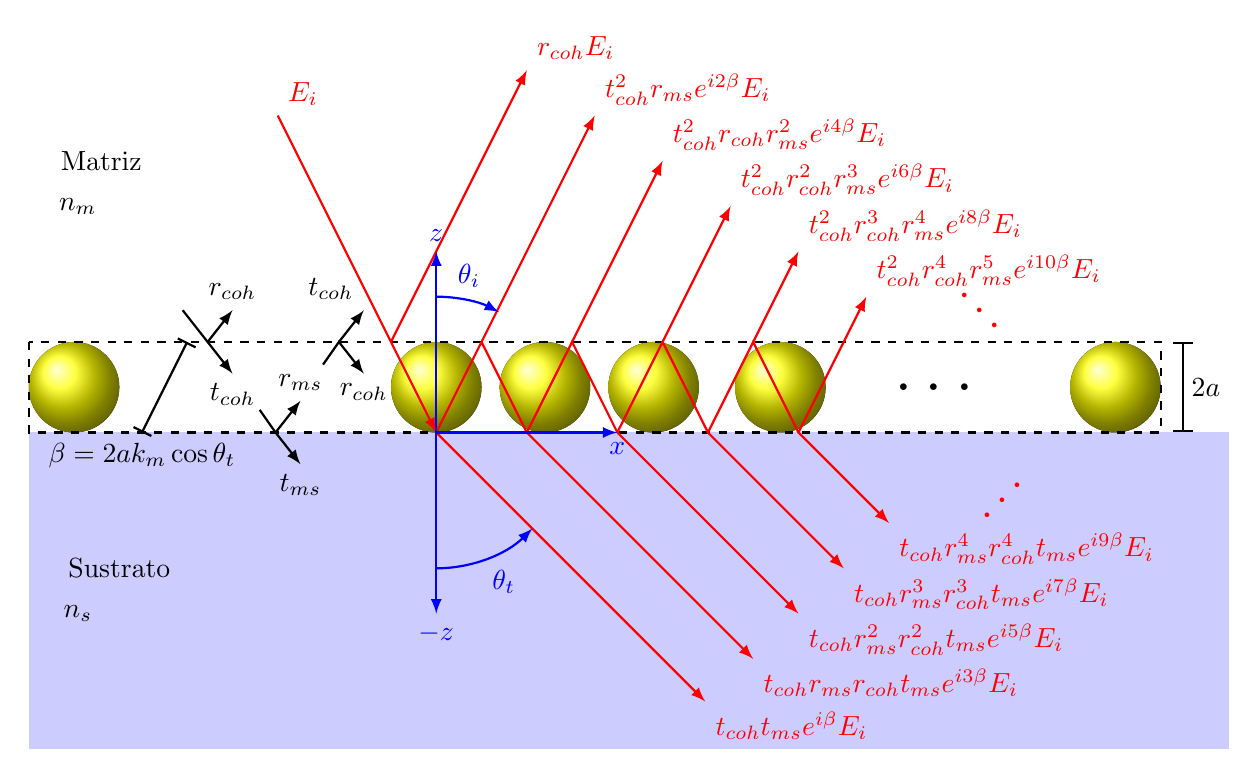
\begin{tikzpicture}[scale=1.15]
\def\a{.5}
\def\d{.5}
\def\t{.3}

\fill[blue, opacity = .2] (-4.5,-3.5) rectangle(8.75,0);

\foreach \x in {-4,0,1.2,2.4,3.8,7.5}{ %-2.9,-1.1
\fill[ball color=yellow, opacity=1] (\x,\d) circle(\a);}

\draw[thick, dashed] (-4.5,2*\d) rectangle (8,0);
\node at (5.5,\d) {\Huge $\ldots$};

%%%%%%%%%%%%%-------------transmisiones

\draw[- latex, thick, red](-135:0)--(-45:4.2) node[anchor=north west]{$t_{coh}t_{ms}e^{i\beta}E_i$};
\draw[- latex, thick, red](0,0)--(1*\d,2*\d)--(2*\d,0)--(3+\d,-3+\d) node[anchor=north west]{$t_{coh}r_{ms}r_{coh}t_{ms}e^{i3\beta}E_i$};
\draw[- latex, thick, red](2*\d,0)--(3*\d,2*\d)--(4*\d,0)--(3+2*\d,-3+2*\d) node[anchor=north west]{$t_{coh}r_{ms}^2r_{coh}^2t_{ms}e^{i5\beta}E_i$};
\draw[- latex, thick, red](4*\d,0)--(5*\d,2*\d)--(6*\d,0)--(3+3*\d,-3+3*\d) node[anchor=north west]{$t_{coh}r_{ms}^3r_{coh}^3t_{ms}e^{i7\beta}E_i$};
\draw[- latex, thick, red](6*\d,0)--(7*\d,2*\d)--(8*\d,0)--(3+4*\d,-3+4*\d) node[anchor=north west]{$t_{coh}r_{ms}^4r_{coh}^4t_{ms}e^{i9\beta}E_i$};
\draw[-, thick, red](8*\d,0)--(9*\d,2*\d);
\node[rotate={45}] at (6.25,-.75) {\color{red}\LARGE $\ldots$};


%%%%%%%%%%%%%-------------reflexiones
\draw[latex -, thick, red](0,0)--(-1.75,3.5) node[anchor=south west]{$E_i$};
\draw[- latex, thick, red](-1*\d,2*\d)--(2-2*\d,4+0*\d) node[anchor=south west]{$r_{coh}E_i$};
\draw[- latex, thick, red](1*\d,2*\d)--(1.75,3.5) node[anchor=south west]{$t_{coh}^2r_{ms}e^{i2\beta}E_i$};
\draw[- latex, thick, red](3*\d,2*\d)--(2+1*\d,4-2*\d) node[anchor=south west]{$ t_{coh}^2r_{coh}r_{ms}^2e^{i4\beta}E_i$};
\draw[- latex, thick, red](5*\d,2*\d)--(2+2.5*\d,4-3*\d) node[anchor=south west]{$ t_{coh}^2r_{coh}^2r_{ms}^3e^{i6\beta}E_i$};
\draw[- latex, thick, red](7*\d,2*\d)--(2+4*\d,4-4*\d) node[anchor=south west]{$ t_{coh}^2r_{coh}^3r_{ms}^4e^{i8\beta}E_i$};
\draw[- latex, thick, red](9*\d,2*\d)--(2+5.5*\d,4-5*\d) node[anchor=south west]{$t_{coh}^2r_{coh}^4r_{ms}^5e^{i10\beta}E_i$};
\node[rotate={-45}] at (6,1.35) {\color{red}\LARGE $\ldots$};



\node at (-4,2.5) {$\; n_m$};
\node at (-3.7,3) {Matriz};
\node at (-4,-2) {$\; n_s$};
\node at (-3.5,-1.5) {Sustrato};

%.55,0
%2,0
%1.2,2*\ḑ
%%\draw[latex - , thick](-2.8,-.5)--(-3.5,.5) node[anchor=north]{$r_{sm},\,t_{sm}$};
\draw[latex - , thick, shift ={(2,2*\d)}](-2.8,-.35)node[anchor=north]{$r_{coh}$}--(-3.075,0)--(-3.25,-.25);
\draw[latex -,thick, shift ={(2,2*\d)}](-2.8,.35)node[anchor=south east]{$t_{coh}$}--(-3.075,0);
\draw[latex - , thick, shift ={(.55,2*\d)}](-2.8,-.35)node[anchor=north]{$t_{coh}$}--(-3.075,0)--(-3.35,.35);
\draw[latex -,thick, shift ={(.55,2*\d)}](-2.8,.35)node[anchor=south]{$r_{coh}$}--(-3.075,0);
\draw[latex - , thick, shift ={(1.3,0)}](-2.8,-.35)node[anchor=north]{$t_{ms}$}--(-3.075,0)--(-3.25,+.25);
\draw[latex -,thick, shift ={(1.3,0)}](-2.8,.35)node[anchor=south]{$r_{ms}$}--(-3.075,0);

\draw[|-|,thick, shift ={(-3.25,0)}](0,0)node[anchor=north]{$\beta = 2ak_m\cos\theta_t$}--(1*\d,2*\d) ;

\draw[|-|,thick, shift ={(8.25,0)}](0,0)--(0,2*\d) ;
\node at (8.5,\d){$2a$};

\draw[- latex, thick, blue] (0,0)--(90:2) node[anchor = south]{$z$};
\draw[- latex, thick, blue] (0,0)--(90:-2) node[anchor = north]{$-z$};
\draw[- latex, thick, blue] (0,0)--(0:2) node[anchor = north]{$x$};
\path (0,0)++(85:1.5)node[anchor=south west, blue]{$\theta_i$}; 
\draw[- latex, thick, blue](90:1.5)arc(90:62.5:1.5);
\path (0,0)++(-70:1.5)node[anchor=north west, blue]{$\theta_t$}; 
\draw[- latex, thick, blue](-90:1.5)arc(-90:-45:1.5);


\end{tikzpicture}
	\caption{ Esquema de las múltiples reflexiones en incidencia externa del sistema matriz-monocapa-sustrato producidos por una onda plana $\vb{E}^i$ que incide sobre una monocapa de NPs esféricas de radio $a$, embebida en una matriz con índice de refracción  $n_m$ y soportada por un sustrato con índice de refracción $n_s$, a un ángulo $\theta_i$ respecto a la dirección normal de la monocapa. Las reflexiones y transmisiones en la interfaz sustrato-matriz ($z=0$) se describen mediante los coeficientes de amplitud de Fresnel [Ecs. \eqref{eq:rs}--\eqref{eq:tp}], mientras que en la interfaz monocapa-matriz ($z=2a$) las reflexiones y transmisiones son descritas por el CSM [Ecs. \eqref{eqs:rtcoh}]. Los coeficientes de amplitud de reflexión y transmisión se evalúan en $\theta_i$. En los coeficientes de amplitud  $r_{\alpha\beta}$ y $t_{\alpha\beta}$ el medio de incidencia de la onda plana monocromática corresponde a $\alpha$ y el de transmisión a $\beta$.}\label{fig:CSM-externa}
	\end{figure}

Para calcular los coeficientes de amplitud de reflexión y transmisión del sistema matriz-monocapa-sustrato, es decir, en incidencia externa, se consideran las múltiples reflexiones del sistema, mostradas en la Fig. \ref{fig:CSM-externa}. Cuando la onda plana con amplitud $E_i$ incide en la monocapa, en $z=2a$, se presenta una primera reflexión dada por el CSM, es decir que la amplitud del campo eléctrico en la primera reflexión es $r_{coh}E_i$. La segunda reflexión se presenta tras dos transmisiones en la monocapa y una reflexión en la interfaz matriz-sustrato, con una diferencia de fase $2\beta=2(2ak_m\cos\theta)$ respecto a la primera reflexión, es decir, que la amplitud de la segunda reflexión es $t_{coh}^2r_{ms}e^{i2\beta}E_i$. En la tercera reflexión hay dos transmisiones en la monocapa, dos reflexiones en la interfaz matriz-sustrato, y una reflexión en la monocapa; al considerar la diferencia de camino óptico con la primera relfexión, la amplitud de la tercera reflexión es $t_{coh}^2r_{coh}r_{ms}^2e^{i4\beta}E_i$. Al considerar el resto de las reflexiones, se obtiene que el coeficiente de amplitud de reflexión $r$ del sistema es \index{Fresnel!coeficientes de amplitud de ($r,t$)}
%
	\begin{align}
	r = r_{coh} +
		 t_{coh}^2r_{ms}e^{i2\beta}+
		 t_{coh}^2r_{coh}r_{ms}^2e^{i4\beta}+
		 t_{coh}^2r_{coh}^2r_{ms}^3e^{i6\beta}+
		 t_{coh}^2r_{coh}^3r_{ms}^4e^{i8\beta}+\ldots
%		 t_{coh}^2r_{coh}^4r_{ms}^5e^{i10\beta}+\ldots\,.
	\label{eq:r_ext_span}
	\end{align}
%
Para el cálculo del coeficiente de amplitud de transmisión $t $ del sistema se sigue un procedimiento análogo al de $r$: la primera transmisión ocurre después de una transmisión en la monocapa, una transmisión en la interfaz matriz-sustrato y una diferencia de fase de $\beta$, por lo que la amplitud de la primera transmisión es $t_{coh}t_{ms}e^{i\beta}$. Para la $m$-ésima transmisión se presentan $m-1$ reflexiones con la monocapa y $m-1$ con el sustrato, además de una fase de $(2m-1)\beta$, es decir,
%
	\begin{align}
	t = t_{coh}t_{ms}e^{i\beta} +
		t_{coh}r_{ms}r_{coh}t_{ms}e^{i3\beta}+
		t_{coh}r_{ms}^2r_{coh}^2t_{ms}e^{i5\beta}+	
		t_{coh}r_{ms}^3r_{coh}^3t_{ms}e^{i7\beta}+ \ldots					
%		t_{coh}r_{ms}^4r_{coh}^4t_{ms}e^{i9\beta}+ \ldots				
%		t_{coh}r_{ms}^5r_{coh}^5t_{ms}e^{i11\beta}+\ldots\,.
	\label{eq:t_ext_span}
	\end{align}\noindent
%	
Al factorizar $r_{ms}t_{coh}^2e^{2i\beta}$ en la Ec. \eqref{eq:r_ext_span}, a excepción del primer término $r_{coh}$, y factorizar $t_{coh}t_{ms}e^{i\beta}$ en la Ec. \eqref{eq:t_ext_span}, se obtienen las siguientes expresiones
%
	\begin{align*}
	r &= r_{coh} + r_{ms}t_{coh}^2e^{2i\beta}\left[1+r_{coh}r_{ms}e^{2i\beta}+\qty(r_{coh}r_{ms}e^{2i\beta})^2+\qty(r_{coh}r_{ms}e^{2i\beta})^3+\ldots,\right]\\
	t &= t_{coh}t_{ms}e^{i\beta} \left[1+r_{coh}r_{ms}e^{2i\beta}+\qty(r_{coh}r_{ms}e^{2i\beta})^2+\qty(r_{coh}r_{ms}e^{2i\beta})^3+\ldots\right] ,
	\end{align*}
%
y dado que $\norm{r_{coh}r_{ms}e^{2i\beta}}<1$, es posible reescribir los coeficientes de amplitud del sistema como\index{Esparcimiento!Coherente, Modelo de (CSM)!coeficientes de amplitud!incidencia externa)} \vspace*{-.75em}\begin{subequations}
%
	\begin{tcolorbox}[title = Coeficientes de amplitud dados por el CSM en incidencia externa, breakable ]
	\eqhalf{r = r_{coh}(\theta_i)+ \frac{r_{ms}(\theta_i)t_{coh}(\theta_i)e^{i2\beta}}
										{1-r_{coh}(\theta_i)r_{ms}(\theta_i)e^{2i\beta}},
	\label{seq:rCSMext}}
	\eqhalf{t = \frac{t_{ms}(\theta_i)t_{coh}(\theta_i)e^{i\beta}}
									{1-r_{coh}(\theta_i)r_{ms}(\theta_i)e^{2i\beta}},
	\label{seq:tCSMext}}
	
	con $\beta = 2a k_0n_m\cos\theta_i$.
	\end{tcolorbox}\label{eqs:rtCSMext}\end{subequations}\vspace*{-.75em}
%

Cuando se considera que la onda plana monocromática incide sobre el sistema con un ángulo $\theta_i$ en una confiuración  ATR, ésta se refleja por la interfaz sustrato-matriz ($z=0$) a un ángulo  $\theta_i$ pero se transmite a un ángulo  $\theta_t$. La onda plana ilumina a las NPs a un ángulo $\theta_t$, y a este mismo ángulo se refleja y transmite a través de la monocapa (en $z=2a$), como se observa en la Fig. \ref{fig:CSM-ATR}, donde, por claridad, los subíndices $sm$ corresponden a los coeficientes de Fresnel evaluados en $\theta_i$, mientras que $ms$ y $coh$, en $\theta_t$. De forma análoga al caso de incidencia externa, los coeficientes de amplitud de reflexión y transmisión del sistema son
%
	\begin{align}
	r &= r_{sm}+ 
		t_{sm}r_{coh}r_{ms}e^{i2\beta}+
		t_{sm}r_{coh}^2r_{ms}e^{i4\beta}+
		t_{sm}r_{coh}^3r_{ms}^2e^{i6\beta}+
		t_{sm}r_{coh}^4r_{ms}^3e^{i8\beta}\ldots,
	\label{eq:r_ATR_span}\\		
	t &= t_{sm}t_{coh}e^{i\beta}+ 
		t_{sm}r_{coh}r_{ms}t_{coh}e^{i3\beta}+
		t_{sm}r_{coh}^2r_{ms}^2t_{coh}e^{i5\beta}+
		t_{sm}r_{coh}^3r_{ms}^3t_{coh}e^{i7\beta}+\ldots,	
%		t_{sm}r_{coh}^4r_{ms}^4t_{coh}e^{i9\beta}+\ldots,	
	\label{eq:t_ATR_span}
	\end{align}
donde $\beta = 2ak_m\cos\theta_t$. Al factorizar $t_{sm}r_{coh}t_{ms}e^{2i\beta}$ en la Ec. \eqref{eq:r_ATR_span} y $t_{sm}t_{coh}e^{i\beta}$ en la Ec. \eqref{eq:t_ATR_span}, y considerar que $\norm{r_{coh}r_{ms}e^{i2\beta}}<1$, los coeficientes de amplitud están dados por \vspace*{-2em}

\begin{figure}[h!]\centering
	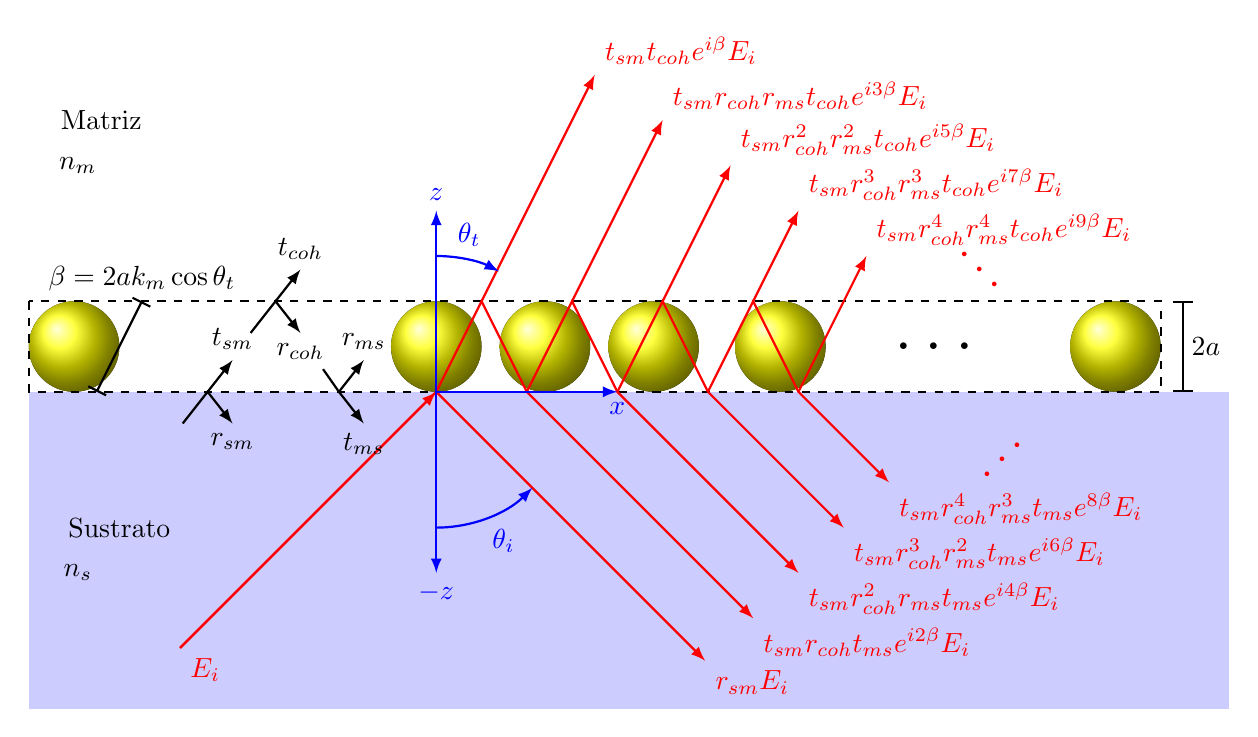
\begin{tikzpicture}[scale=1.15]
\def\a{.5}
\def\d{.5}
\def\t{.3}

\fill[blue, opacity = .2] (-4.5,-3.5) rectangle(8.75,0);

\foreach \x in {-4,0,1.2,2.4,3.8,7.5}{ %-2.9,-1.1
\fill[ball color=yellow, opacity=1] (\x,\d) circle(\a);}

\draw[thick, dashed] (-4.5,2*\d) rectangle (8,0);
\node at (5.5,\d) {\Huge $\ldots$};


%%%%%%%%%%%%%-------------Reflexiones
%
%\draw[latex -, thick, red](-135:0)--(-135:4) node[anchor=north]{$E_i$};
%\draw[- latex, thick, red](-135:4)--(-135:0)--(-45:4) node[anchor=north]{$r_{coh}E_i$};
%\draw[- latex, thick, red](0,0)--(2*\d,2*\d)--(3+2*\d,-3+2*\d) node[anchor=south west]{$t_{coh}r_{ms}t_{coh}E_i$};
%\draw[- latex, thick, red](4*\d,0)--(6*\d,2*\d)--(3+6*\d,-3+2*\d) node[anchor=south west]{$r_{coh}E_i$};


\draw[latex -, thick, red](-135:0)--(-135:4) node[anchor=north west]{$E_i$};
\draw[- latex, thick, red](-135:4)--(-135:0)--(-45:4.2) node[anchor=north west]{$r_{sm}E_i$};
\draw[- latex, thick, red](0,0)--(1*\d,2*\d)--(2*\d,0)--(3+\d,-3+\d) node[anchor=north west]{$t_{sm}r_{coh}t_{ms}e^{i2\beta}E_i$};
\draw[- latex, thick, red](2*\d,0)--(3*\d,2*\d)--(4*\d,0)--(3+2*\d,-3+2*\d) node[anchor=north west]{$t_{sm}r_{coh}^2r_{ms}t_{ms}e^{i4\beta}E_i$};
\draw[- latex, thick, red](4*\d,0)--(5*\d,2*\d)--(6*\d,0)--(3+3*\d,-3+3*\d) node[anchor=north west]{$t_{sm}r_{coh}^3r_{ms}^2t_{ms}e^{i6\beta}E_i$};
\draw[- latex, thick, red](6*\d,0)--(7*\d,2*\d)--(8*\d,0)--(3+4*\d,-3+4*\d) node[anchor=north west]{$t_{sm}r_{coh}^4r_{ms}^3t_{ms}e^{8\beta}E_i$};
\draw[-, thick, red](8*\d,0)--(9*\d,2*\d);
\node[rotate={45}] at (6.25,-.75) {\color{red}\LARGE $\ldots$};

%%%%%%%%%%%%%-------------transmisiones
\draw[- latex, thick, red](1*\d,2*\d)--(1.75,3.5) node[anchor=south west]{$t_{sm}t_{coh}e^{i\beta}E_i$};
\draw[- latex, thick, red](3*\d,2*\d)--(2+1*\d,4-2*\d) node[anchor=south west]{$t_{sm}r_{coh}r_{ms}t_{coh}e^{i3\beta}E_i$};
\draw[- latex, thick, red](5*\d,2*\d)--(2+2.5*\d,4-3*\d) node[anchor=south west]{$t_{sm}r_{coh}^2r_{ms}^2t_{coh}e^{i5\beta}E_i$};
\draw[- latex, thick, red](7*\d,2*\d)--(2+4*\d,4-4*\d) node[anchor=south west]{$t_{sm}r_{coh}^3r_{ms}^3t_{coh}e^{i7\beta}E_i$};
\draw[- latex, thick, red](9*\d,2*\d)--(2+5.5*\d,4-5*\d) node[anchor=south west]{$t_{sm}r_{coh}^4r_{ms}^4t_{coh}e^{i9\beta}E_i$};
\node[rotate={-45}] at (6,1.35) {\color{red}\LARGE $\ldots$};



\node at (-4,2.5) {$\; n_m$};
\node at (-3.7,3) {Matriz};
\node at (-4,-2) {$\; n_s$};
\node at (-3.5,-1.5) {Sustrato};

%\draw[latex - , thick](-2.8,-.5)--(-3.5,.5) node[anchor=north]{$r_{sm},\,t_{sm}$};
\draw[latex - , thick, shift ={(.55,0)}](-2.8,-.35)node[anchor=north]{$r_{sm}$}--(-3.075,0)--(-3.35,-.35);
\draw[latex -,thick, shift ={(.55,0)}](-2.8,.35)node[anchor=south]{$t_{sm}$}--(-3.075,0);
\draw[latex - , thick, shift ={(2.0,0)}](-2.8,-.35)node[anchor=north]{$t_{ms}$}--(-3.075,0)--(-3.25,.25);
\draw[latex -,thick, shift ={(2.0,0)}](-2.8,.35)node[anchor=south]{$r_{ms}$}--(-3.075,0);
\draw[latex - , thick, shift ={(1.3,2*\d)}](-2.8,-.35)node[anchor=north]{$r_{coh}$}--(-3.075,0)--(-3.35,-.35);
\draw[latex -,thick, shift ={(1.3,2*\d)}](-2.8,.35)node[anchor=south]{$t_{coh}$}--(-3.075,0);

\draw[|-|,thick, shift ={(-3.75,0)}](0,0)--(1*\d,2*\d) node[anchor=south]{$\beta = 2ak_m\cos\theta_t$};

\draw[|-|,thick, shift ={(8.25,0)}](0,0)--(0,2*\d) ;
\node at (8.5,\d){$2a$};

\draw[- latex, thick, blue] (0,0)--(90:2) node[anchor = south]{$z$};
\draw[- latex, thick, blue] (0,0)--(90:-2) node[anchor = north]{$-z$};
\draw[- latex, thick, blue] (0,0)--(0:2) node[anchor = north]{$x$};
\path (0,0)++(85:1.5)node[anchor=south west, blue]{$\theta_t$}; 
\draw[- latex, thick, blue](90:1.5)arc(90:62.5:1.5);
\path (0,0)++(-70:1.5)node[anchor=north west, blue]{$\theta_i$}; 
\draw[- latex, thick, blue](-90:1.5)arc(-90:-45:1.5);


\end{tikzpicture}
	\caption{ Esquema de las múltiples reflexiones en ATR del sistema matriz-monocapa-sustrato producidos por una onda plana $\vb{E}^i$ que incide en la interfaz de un sustrato, con índice de refracción $n_s$, que sostiene a una monocapa de NPs esféricas de radio $a$ embebida en una matriz con $n_m$, a un ángulo $\theta_i$ respecto a la dirección normal a la interfaz. Las reflexiones y transmisiones en la interfaz sustrato-matriz ($z=0$) se describen por los coeficientes de amplitud de Fresnel [Ecs. \eqref{eq:rs}--\eqref{eq:tp}] en $\theta_i$, mientras que en la interfaz monocapa-matriz ($z=2a$) las reflexiones y transmisiones son descritas por el CSM [Ecs. \eqref{eqs:rtcoh}] en $\theta_t$. En los coeficientes de amplitud  $r_{\alpha\beta}$ y $t_{\alpha\beta}$ el medio de incidencia del haz de luz es $\alpha$ y el de transmisión en $\beta$.}\label{fig:CSM-ATR}
	\end{figure}



	\begin{align}
	r =& r_{sm} + t_{sm}r_{coh}t_{ms}e^{2i\beta}\left[1+r_{coh}r_{ms}e^{2i\beta}+\qty(r_{coh}r_{ms}e^{2i\beta})^2+\qty(r_{coh}r_{ms}e^{2i\beta})^3+\ldots,\right] \notag \\
		=& r_{sm} + \frac{ t_{sm}r_{coh}t_{ms}e^{2i\beta}}
				{1-r_{ms}r_{coh}e^{i2\beta}}, \label{eq:r_ATR_preStokes} \\
	t =& t_{coh}t_{ms}e^{i\beta} \left[1+r_{coh}r_{ms}e^{2i\beta}+\qty(r_{coh}r_{ms}e^{2i\beta})^2+\qty(r_{coh}r_{ms}e^{2i\beta})^3+\ldots\right]
	=\frac{  t_{coh}t_{ms}e^{i\beta} }
				{1-r_{ms}r_{coh}e^{i2\beta}}.\notag
	\end{align}
%
Es posible reescribir la Ec. \eqref{eq:r_ATR_preStokes} empleando las relaciones de Stokes\footnote{Las relaciones de Stokes\index{Fresnel!coeficientes de amplitud de ($r,t$)!relaciones de Stokes} se deducen a partir de la invariancia de las ecuaciones de Maxwell ante inversiones temporales ($t\to -t$), y relacionan a los coeficientes de amplitud $r$ y $t$ evaluados en $\theta_i$ y $\theta_t$ para una interfaz entre medios no absorbentes. Las relaciones de Stokes son \cite{hecht1998optics,garcia2012multiple} $r_{it}(\theta_i) = -r_{ti}(\theta_t)$, $t_{it}(\theta_i) = 1+r_{it}(\theta_i)$, y $t_{ti}(\theta_t) = 1+r_{it}(\theta_t)$.}, por lo que se obtiene\index{Esparcimiento!Coherente, Modelo de (CSM)!coeficientes de amplitud!incidencia interna} \begin{subequations}\vspace*{-.75em}
%
\begin{tcolorbox}[title = Coeficientes de amplitud de CSM en configuración ATR, breakable ]
	\eqhalf{r = \frac{r_{sm}(\theta_i)+r_{coh}(\theta_t)e^{i2\beta}}
					{1-r_{coh}(\theta_t)r_{sm}(\theta_i)e^{2i\beta}},
	\label{seq:rCSMATR}}
	\eqhalf{t = \frac{t_{sm}(\theta_i)t_{coh}(\theta_t)e^{i\beta}}
									{1-r_{coh}(\theta_t)r_{ms}(\theta_t)e^{2i\beta}},
	\label{seq:tCSMATR}}
	
	con $\beta = 2a k_0n_m\cos\theta_t$.
	\end{tcolorbox}\label{eqs:rtCSMATR}\end{subequations}\vspace*{-.75em}






\chapter{Resultados numéricos}

Para estudiar la respuesta electromagnética (EM) de una monocapa de nanopartículas (NPs) inmersa en un medio dieléctrico, denominado matriz, y soportada sobre un sustrato dieléctrico, se emplea el formalismo del modelo de esparcimiento coherente (Coherent Scattering Model, CSM) para calcular la reflectanci $R$ y transmistancia $T$ del sistema. El CSM que proporciona expresiones analíticas de los coeficientes de amplitud de reflexión $r$ y transmisión $t$ de la monocapa cuando está suspendida en el espacio libre (Free Stanting Monolayer, FSM) [Ecs. \eqref{eqs:rtcoh}], y para el sistema matriz-monocapa-sustrato tanto en incidencia externa [Ecs. \eqref{eqs:rtCSMext}] como en una configuración de reflexión total atenuada \index{Reflexión total!atenuada} (Attenuated Total Reflection, ATR) [Ecs. \eqref{eqs:rtCSMATR}].

En la primera sección de este capítulo se calcula la respuesta EM de una moncapa de NPs esféricas, cuya  función dieléctrica $\varepsilon(\omega)$ se describe mediante el modelo de Drude-Sommerfeld [Ec. \eqref{eq:Drude}], dado que depende sólo de dos parámetros: la frecuencia de plasma $\omega_p$ y la constante fenomenológica de amortiguamiento $\gamma$. La elección de los parámetros $\omega_p$ y $\gamma$ sintoniza las resonancias plasmónicas de superficie (Surface Plasmon Resonances, SPRs) Y ajusta el ancho de cada una de ellas, evitando el traslape y facilitando la identificación de cada modo de manera individual. De esta forma, en el cálculo de la reflectancia y transmitancia de un sistema conformado por un sustrato, una matriz y una monocapa de NPs, es posible identificar la presencia de algún otro modo  distinto distinto a las SPRs de partículas individuales (Single Particles SPR, SP-SPRs), como el \emph{modo guiado} reportado en \cite{kabashin2009plasmonic} y \cite{danilov2018ultra}. En la segunda sección se emplean las correcciones por tamaño para partículas esféricas de las funciones dieléctricas del oro y de la plata para identificar si un modo semejante al modo guiado se encuentra en materiales reales.

\section{Resultados con el modelo de Drude-Sommerfeld}

 En la primera subsección se analiza la reflectancia de una FSM empleando el modelo de Drude-Sommerfled con parámetros $\omega_p = 4.3$ eV y  $\gamma = 0.15$ eV [ver Fig. \ref{sfig:Drude4eV}], y comparando la respuesta EM de la monocapa con la de una partícula individual. En la segunda subsección se estudia la reflectancia de una monocapa soportada en configuración de reflexión interna atenuada, ver Fig. \ref{fig:ATR}, empleando el modelo de Drude-Sommerfeld en un primer caso con los parámetros  $\omega_p = 4.3$ eV y  $\gamma = 0.15$, y en uno segundo con $\omega_p = 10$ eV y $\gamma = 0.15$  [ver Fig. \ref{sfig:Drude10eV}]; posteriormente se calculó la reflectancia de la monocapa considerando  variaciones en la fracción de cubierta $\Theta$ y el radio de las NPs $a$, parámetros que modifican las proporciones del sistema, tales como la distancia promedio entre las NPs, y la cantidad de electrones libres sobre la monocapa. Adicional al cálculo de la reflectancia, se calculó la transmitancia de la monocapa para las dos funciones dieléctricas, $\omega_p =4.3$ eV y $\omega_p =10$ eV, para corroborar que los modos distintos a las SP-SPRs tienen un comportamiento semejante a un modo guiado. 
	
	\subsection{Reflectancia de una monocapa suspendida en aire}
	
Para el cálculo de la reflectancia mediante el CSM de una FSM suspendida en aire ($n_m=1$), se empleó la Ec.  \eqref{eq:R} con el coeficiente de amplitud de reflexión coherente $r_{coh}$ [Ec.  \eqref{seq:rcoh}].  En la Fig.  \ref{fig:R-FSM} se muestran los resultados de la reflectancia $R$ como función del ángulo de incidencia $\theta_i$ y tanto de la longitud de onda $\lambda$ del haz incidente (escala inferior), así como de la energía del haz incidente en unidades de $\hbar\omega = h c /\lambda$ (escala superior).  La frecuencia de plasma empleada para la función dieléctrica tipo Drude fue $\omega_p = 4. 3$ eV y la constante fenomenológica de amortiguamiento $\gamma = 0. 15$ eV (que corresponden a $288. 5$ nm  y $8,270$ nm respectivamente). Se consideraron NPs de radio $a=30$ nm y fracciones de cubierta $\Theta$: $0. 05$, $0. 1$, $0. 2$, $0. 3$ y $0. 4$. En el renglón superior de la Fig. \ref{fig:R-FSM}, gráficas de $\mathbf{i)}$ a $\mathbf{v)}$, se muestra la reflectancia para polarización \emph{p}, mientras que en el renglón inferior se presentan las gráficas, de $\mathbf{vi)}$ a $\mathbf{x)}$, de la reflectancia para polarización \emph{s}. La línea punteada vertical verde  en $\lambda \approx 526$ nm corresponde a la SP-SPR de partícula individual dipolar ($\ell = 1$), mientras que la línea vertical rosa punteada en $\lambda \approx 462$ nm corresponde a la excitación del modo cuadrupolar ($\ell=2$).
					
	\begin{figure}[h!]\centering
\includegraphics[width = .9\linewidth	]{2-Resultados/figs/4-Wp4FSMThetaVar/0-2D_Grid.png}%
\includegraphics[scale=.85, trim={00 -5 00 00}, clip]{2-Resultados/figs/0-RBar_v}\vspace*{-1em}
	\caption{Gráficas de reflectancia para una FSM como función del ángulo de incidencia $\theta_i$ y tanto de la longitud de onda $\lambda$ (escala inferior), como de la energía del haz incidente en unidades de $\hbar\omega$ (escala superior), para una función dieléctrica tipo Drude con $\omega_p=4. 3$ eV  y  $\gamma=0. 15$ eV.  Las gráficas   en el renglón superior [$\mathbf{i)-v)}$]  muestran los resultados de reflectancia para  polarización \emph{p} y las del renglón inferior  [$\mathbf{i)-v)}$] para polarización  \emph{s}, donde se consideraron NPs de radio $a=30$ nm y distintas fracciones de cubierta $\Theta$: $0. 05$, $0. 1$, $0. 2$, $0. 3$ y $0. 4$. Las líneas verticales punteadas verdes y rosas corresponden a las SP-SPRs dipolar ($526$ nm) y cuadrupolar ($462$ nm), respectivamente.}	\label{fig:R-FSM}	
	\end{figure}		
					
La reflectancia para polarización \emph{p} [Fig. \ref{fig:R-FSM} $\mathbf{i)-v)}$] es cero para el ángulo de Brewster $\theta_B \approx 45^\circ$ y para regiones alejadas de las SP-SPRs (líneas punteadas verticales verde y rosa  localizadas en $526$ nm y $462$ nm, respectivamente). En la gráfica \textbf{v)}, $\Theta=0.4$,  se observa a $526$ nm (escala inferior) extinción de luz alrededor y, en la región al rededor de esta longitud de onda, la reflectancia comienza a aumentar. Conforme la fracción de cubierta disminuye, gráficas \textbf{iii)} y \textbf{iv)}, la extinción de luz es  menos evidente en $526$ nm y para las fracciones de cubierta $\Theta=0.05$ y $0.1$, gráficas \textbf{i)} y \textbf{ii)}, ya no es apreciable la extinción de luz a la frecuencia de la SP-SPR dipolar. En contraparte, para polarización \emph{s} [Fig. \ref{fig:R-FSM} $\mathbf{vi)-x)}$] la reflectancia es apreciable para todo ángulo de incidencia a las frecuencias de las SP-SPRs . Para ambas polarizaciones se observa que mientras la fracción de cubierta aumenta,  crece la región donde la reflectancia es apreciable, así como los valores calculados de $R$, evidenciando la presencia de las NPs en la monocapa.

En la Fig. \ref{fig:FSM-Cuts} se muestran cortes de la reflectancia graficada en la Fig. \ref{fig:R-FSM} para un ángulo de incidencia $\theta_i = 65^\circ$, tanto para un haz incidente con polarización \emph{p} [Fig. \ref{sfig:FSM-cutp}], como uno con polarización \emph{s} [Fig. \ref{sfig:FSM-cuts}]. Para la polarización \emph{p} se presenta un mínimo en la reflectancia alrededor de $526$ nm para fracciones de cubierta mayores a $\Theta = 0.05$. Los mínimos de $R_p$ a la frecuencia de la SP-SPR dipolar son más pronunciados conforme aumenta la fracción de cubierta sin embargo, para $\Theta=0.05$ se observa un máximo en lugar de un mínimo. Para polarización \emph{s}, se presenta un máximo en la reflectancia a $526$ nm para todos los valores de $\Theta$. Para las fracciones de cubierta mayores, $\Theta = 0.3$ y $\Theta = 0.4$,  se observa un  mínimo en la reflectancia alrededor de $462$ nm para ambas polarizaciones, lo que corresponde a la SP-SPR cuadrupolar.

		\begin{figure}[h!]\centering\hspace*{-1.5em}
	\begin{subfigure}{.01\linewidth}\caption{}\label{sfig:FSM-cutp}\vspace{4.5cm}\end{subfigure}
	\begin{subfigure}{.45\linewidth}\hspace*{-1.5em}
	\includegraphics[scale=1]{2-Resultados/figs/4-Wp4FSMThetaVar/cut_angle_65_p.pdf}\end{subfigure}
	\begin{subfigure}{.01\linewidth}\caption{}\label{sfig:FSM-cuts}\vspace{4.5cm}\end{subfigure}\hspace*{-1.em}
	\begin{subfigure}{.45\linewidth}\centering
	\includegraphics[scale=1 ]{2-Resultados/figs/4-Wp4FSMThetaVar/cut_angle_65_s.pdf}\end{subfigure}\vspace*{-.7em}
	\caption{Cortes de la Fig. \ref{fig:R-FSM} a $\theta_i = 65^\circ$ de reflectancia de una FSM de NPs esféricas de radio $a=30$ nm en polarización \textbf{a)} \emph{p} y \textbf{b)} \emph{s} como función tanto de la longitud de onda $\lambda$ (escala inferior), como de la energía del haz incidente en unidades de $\hbar\omega$ (escala superior). Los parámetros de la función dieléctrica tipo Drude para las NPs son $\omega_p = 4.3$ eV y $\gamma = 0.15$ eV y las fracciones de cubierta consideradas fueron $\Theta$: $0. 05$, $0. 1$, $0. 2$, $0. 3$ y $0. 4$. Las líneas verticales punteadas verdes y rosas corresponden a las SP-SPRs dipolar ($526$ nm) y cuadrupolar ($462$ nm), respectivamente.}\label{fig:FSM-Cuts}
	\end{figure}	

Al calcular la distancia promedio $\langle d \rangle$ entre las NPs  de $a = 30$ nm mediante la Tab. \eqref{tab:MeanD}, se obtiene que $\langle d \rangle = 177.8$ nm para $\Theta = 0.05$, $\langle d \rangle = 105.1$ nm para $\Theta = 0.1$ y $\langle d \rangle = 24.1$ nm para $\Theta = 0.4$. El análisis de una partícula individual es válido para el caso de $\Theta=0.05$ (en negro en la Fig. \ref{fig:FSM-Cuts}), debido a la distancia promedio entre las NPs, por tanto, la presencia del máximo en la reflectancia en la SP-SPRs dipolar (línea punteada vertical verde) corresponde a una cota mínima en $R_p$ debido al esparcimiento de cada una de las NPs; en la Fig. \ref{sig:ScatDiag-Drude4} se grafica el diagrama de esparcimiento de una partícula esférica en la monocapa . Conforme el número de NPS aumenta, la luz esparcida también lo hace sin embargo, la extinción de luz es causada en su mayoría por la absorción, como se observa en la Fig. \ref{sfig:Q-ext-Drude4}, por lo que también se llega a una

	

En las Figs. \ref{fig:R-FSM} y \ref{fig:FSM-Cuts} se observa la respuesta EM de una monocapa de NPs suspendida en vacío al interactuar con una onda plana. Si se considera la presencia de un sustrato que soporte la monocapa, se puede estar en configuraci\'on de incidencia externa o interna seg\'un sea el medio de incidencia de la onda plana. Para incidencia externa, a todo ángulo de incidencia,  una onda plana ilumina a las NPs de la monocapa por lo que, respecto al caso de la FSM, la posición de lo máximos y mínimos de la reflectancia no cambiarán y los valores de $R$ presentarán un decrecimiento. Por otro lado, para el caso de incidencia interna y ángulos mayores al ángulo crítico $\theta_c = \arcsin(n_m/n_s)$, las NPs en la monocapa son iluminadas por ondas evanescentes, por tratarse de un configuración en ATR, por lo que es posible excitar los plasmones de superficie en las NPs a frecuencias específicas y por tanto observar cambios en la respuesta EM de la monocapa.

	\subsection{Reflectancia y transmitancia de una monocapa en configuración de reflexión total atenuada}

La respuesta EM de una monocapa de NPs suspendida en una matriz con índice de refracción $n_m$ y soportada por un sustrato con índice de refracción $n_s$, se calcula al emplear la Ec.  \eqref{eq:R} con el coeficiente de amplitud de reflexión $r$ de la Ec.  \eqref{seq:rCSMATR}. Para comparar los resultados de la reflectancia $R$ para una FSM y una monocapa en configuración ATR, se emplean los parámetros utilizado en los cálculos de las Figs. \ref{fig:R-FSM} y \ref{fig:FSM-Cuts} ($n_m=1$ , $a=30$ nm, $\omega_p=4.3$ eV y  $\gamma = 0.15$ eV) considerando un sustrato con índice de refracción $n_s=1.5$. En la Fig.  \ref{fig:R-ATR4} se presentan los resultados de la reflectancia $R$ como función del ángulo de incidencia $\theta_i$ y tanto de la longitud de onda $\lambda$ del haz incidente (escala inferior), así como de la energía del haz $\hbar\omega$ (escala superior). Los resultados para polarización \emph{p} se muestran en las gráficas $\mathbf{i)-v)}$ en la Fig.  \ref{fig:R-ATR4} y para polarización \emph{s} en las gráficas $\mathbf{vi)-x)}$. Al igual que para la FSM, se consideraron los casos para la fracción de cubierta $\Theta = 0.05,\,0.1,\,0.2,\,0.3$ y $0.4$. Las SP-SPRs corresponden a la línea vertical verde punteada en $\lambda \approx 526$ nm para el modo dipolar y la línea vertical rosa punteada en  $\lambda \approx 462$ nm para el modo cuadrupolar. Adicionalmente, los puntos amarillos en la Fig. \ref{fig:R-ATR4} corresponden a los mínimos en $R$ para ángulos mayores a $\theta_c\approx 41^\circ$ y longitudes de onda mayores a la SP-SPRs dipolar.

	\begin{figure}[h!]\centering
\includegraphics[width = .9\linewidth, trim={00 00 00 00}, clip	]{2-Resultados/figs/1-Wp4ThetaVar/0-2D_Grid}%
\includegraphics[scale=.85, trim={00 -5 00 00}, clip]{2-Resultados/figs/0-RBar_v}
	\caption{Gráficas de reflectancia de una monocapa en configuración ATR como función del ángulo de incidencia $\theta_i$ y de la longitud de onda $\lambda$ (escala inferior), así como de la energía del haz incidente en unidades de $\hbar\omega$ (escala superior), para una función dieléctrica tipo Drude con $\omega_p=4. 3$ eV  y  $\gamma=0. 15$ eV.  Las gráficas   en el renglón superior [$\mathbf{i)-v)}$]  muestran los resultados de reflectancia para  polarización \emph{p} y las del renglón inferior  [$\mathbf{vi)-x)}$] para polarización  \emph{s}, donde se consideraron NPs de radio $a=30$ nm y distintas fracciones de cubierta $\Theta$: $0. 05$, $0. 1$, $0. 2$, $0. 3$ y $0. 4$. Las líneas verticales punteadas verdes y rosas corresponden a las SP-SPRs dipolar ($526$ nm) y cuadrupolar ($462$ nm), respectivamente.	os puntos amarillos corresponden a los mínimos en $R$ para ángulos mayores a $\theta_c\approx 41^\circ$ y longitudes de onda mayores a la SP-SPRs dipolar.}	\label{fig:R-ATR4}	
	\end{figure}	


En la Fig.  \ref{fig:R-ATR4} la reflectancia para ángulos mayores al ángulo crítico, $\theta_c \approx 41^\circ $ para una interfaz vidrio-aire, es igual a la unidad excepto en dos regiones: alrededor de las longitudes de onda correspondientes a las SP-SPRs (líneas punteadas verticales) y en una región a longitudes de onda mayores a la SP-SPR dipolar (puntos amarillos). La disminución en la reflectancia después del ángulo crítico alrededor de las SP-SPRs es resultado de la extinción debido a las NPs y, al considerar la interacción entre ellas, así como con el sustrato, puede presentarse un corrimiento al rojo, o al azul, de la SPR que, además, depende del ángulo de incidencia del haz, como se observa en las gráficas \textbf{iii)--v)}. La extinción a las longitudes de onda cercanas a las SP-SPRs es más evidente para las fracciones de cubierta más grandes consideradas, por ejemplo, en el panel superior de la Fig. \ref{fig:R-ATR4}, la reflectancia $R_p$ toma valores más cercanos al cero en la gráfica $\mathbf{v)}$, $\Theta = 0.4$,  en comparación a la gráfica $\mathbf{i)}$, $\Theta = 0.05$. A pesar de que este comportamiento es análogo para la polarización \emph{s}, panel inferior de la  Fig. \ref{fig:R-ATR4}, los valores de $R_s$ a las frecuencias de las SP-SPRs son mayores que los de $R_p$, como se observa al comparar las gráficas de los cálculos con $\Theta=0.3$ \textbf{iv)}, $R_p$, y \textbf{ix)}, $R_s$.


Adicional a la región cercana a las SP-SPRs, se observa una región en donde la luz es reflejada con una intensidad, relativa a la intensidad del haz incidente, menor a la unidad, que corresponde a los puntos amarillos en los mínimos de la reflectancia para ángulos de incidencia mayores al ángulo crítico y para longitudes de onda mayores a la SP-SPR dipolar. La separación entre las SP-SPRs y los mínimos a longitudes de ondas mayores (puntos amarillos) aumenta conforme lo hace la fracción de cubierta $\Theta$; este comportamiento es más evidente en polarización \emph{p} que en \emph{s} [ver \textbf{v)} y \textbf{x)} en la Fig.  \ref{fig:R-ATR4}].  Dado que los puntos amarillos corresponden a una excitación que ocurre energías  menores en comparación a las de partículas individuales, se especula que la excitación se debe a una respuesta colectiva como la PSLR reportada en \cite{danilov2018ultra}.
  
  En la Fig. \ref{fig:R-ATR4-Cuts} se presentan cortes para $\theta_i = 65^\circ$ de la reflectacia graficada en la Fig. \ref{fig:R-ATR4} para todas las fracciones de cubierta consideradas; las líneas punteadas verticales corresponden a las longitudes de onda de las SP-SPRs (verde para la excitación dipolar y rosa para la cuadrupolar). En polarización \emph{p}, Fig. \ref{sfig:R-ATR4-cutp}, la excitación de la monocapa para $\Theta=0.05$ alrededor de $\lambda \approx 462$ nm coincide con la SP-SPR cuadrupolar y conforme la fracción de cubierta aumenta, la excitación de la monocapa presenta un corrimiento al azul. En polarización \emph{s}, Fig. \ref{sfig:R-ATR4-cuts},  la SP-SPR cuadrupolar se observa en la respuesta de la monocapa para todas las fracciones de cubierta. La reflectancia, para ambas polarizaciones, en la longitud de onda de la SP-SPR cuadrupolar disminuye conforme la fracción de cubierta crece, por lo que se relaciona con la cantidad de NPs presentes en la monocapa.
  
		\begin{figure}[h!]\centering\hspace*{-1.5em}
	\begin{subfigure}{.01\linewidth}\caption{}\label{sfig:R-ATR4-cutp}\vspace{4.5cm}\end{subfigure}
	\begin{subfigure}{.45\linewidth}\hspace*{-1.5em}
	\includegraphics[scale=1]{2-Resultados/figs/1-Wp4ThetaVar/cut_angle_65_p.pdf}\end{subfigure}
	\begin{subfigure}{.01\linewidth}\caption{}\label{sfig:R-ATR4-cuts}\vspace{4.5cm}\end{subfigure}\hspace*{-1.em}
	\begin{subfigure}{.45\linewidth}\centering
	\includegraphics[scale=1 ]{2-Resultados/figs/1-Wp4ThetaVar/cut_angle_65_s.pdf}\end{subfigure}\vspace*{-.7em}
	\caption{Cortes de la Fig. \ref{fig:R-ATR4} a $\theta_i = 65^\circ$ de reflectancia de una monocapa en configuración ATR de NPs esféricas de radio $a=30$ nm en polarización \textbf{a)} \emph{p} y \textbf{b)} \emph{s} como función de la longitud de onda $\lambda$ (escala inferior) y de la energía $\hbar \omega$ (escala superior). Los parámetros de la función dieléctrica tipo Drude para las NPs son $\omega_p = 4.3$ eV y $\gamma = 0.15$ eV y las fracciones de cubierta consideradas fueron $\Theta$: $0. 05$, $0. 1$, $0. 2$, $0. 3$ y $0. 4$. Las líneas verticales punteadas verdes y rosas corresponden a las SP-SPRs dipolar ($526$ nm) y cuadrupolar ($462$ nm), respectivamente. }\label{fig:R-ATR4-Cuts}
	\end{figure}	
	
    
A diferencia de la SP-SPR cuadrupolar, la excitación dipolar de partícula individual ($526$ nm) no es observable para todos los casos presentados en la Fig. \ref{fig:R-ATR4-Cuts}. En la respuesta óptica de la monocapa sólo se presenta una excitación cercana a la SP-SPR dipolar para los resultados de $R_p$ y para las fracciones de cubierta $\Theta = 0.1,\,0.2,\,0.3$ y $0.4$. Esta excitación se corre al azul conforme $\Theta$ aumenta, al igual que la SP-SPRs cadrupolar. Sin emabargo, se observa una excitación a longitudes de onda mayores a la SP-SPR dipolar para ambas polarizaciones.
 
Los mínimos a longitudes de onda mayores a $530$ nm, para ambas polarizaciones, presentan un corrimiento al rojo conforme la fracción de cubierta de la monocapa aumenta, contrario al comportamiento observado en las excitaciones de la monocapa cercanas a las SP-SPRs. Otra diferencia entre las excitaciones en $\lambda$ mayores a las SP-SPRs y los corrimientos al azul de éstas es que la disminución en el valor de $R$ no es monotona, sino que el decrecimiento en $R$ es máximo a fracciones de cubierta media, como $\Theta=0.2$, que es el valor donde la reflectancia es menor. Por lo anterior, los mínimos en $R_p$ y $R_s$ localizados a longitudes de onda mayores a la de los modos plasmónicos de partícula individual no son corrimientos de las excitaciones multipolares de una partícula, sino que se asocian a una respuesta colectiva de las NPs en la monocapa, más apreciable para la polarización \emph{p} que para \emph{s}.

Es posible separar las resonancias del presunto modo colectivo de las SP-SPRs al incrementar la frecuencia de plasma en el modelo de Drude, que caracteriza la respuesta EM de las NPs. Al considerar $\omega_p = 10$ eV las SP-SPRs se corren al azul, por lo que pueden distinguirse del presunto modo colectivo. Los resultados de la reflectancia de un sistema monocapa con los parámetros empleados en la Fig. \ref{fig:R-ATR4}, pero con $\omega_p = 10$ eV, se muestran en la Fig. \ref{fig:R-ATR10}. Adicional a la SP-SPR dipolar y cuadrupolar (líneas verticales punteadas verde y rosa en $265$ nm y $211$ nm, respectivamente), la SP-SPR octopolar ($\ell = 3$) se muestra en las gráficas mediante la línea vertical punteada cian en $195$ nm, al igual que el presunto modo colectivo que corresponde a los puntos amarillos.
	
  	\begin{figure}[h!]\centering
\includegraphics[width = .9\linewidth]{2-Resultados/figs/2-Wp10ThetaVar/0-2D_Grid.png}%
\includegraphics[scale=.85, trim={00 -5 00 00}, clip]{2-Resultados/figs/0-RBar_v}
	\caption{Gráficas de reflectancia de una monocapa en configuración ATR como función del ángulo de incidencia $\theta_i$ y de la longitud de onda $\lambda$ (escala inferior), así como de la energía del haz incidente en unidades de $\hbar\omega$ (escala superior), para una función dieléctrica tipo Drude con $\omega_p=10$ eV  y  $\gamma=0. 15$ eV.  Las gráficas   en el renglón superior [$\mathbf{i)-v)}$] muestran los resultados  para  polarización \emph{p} y las del renglón inferior  [$\mathbf{vi)-x)}$] para polarización  \emph{s}, donde se consideraron NPs de radio $a=30$ nm y distintas fracciones de cubierta $\Theta$: $0. 05$, $0. 1$, $0. 2$, $0. 3$ y $0. 4$. Las líneas verticales punteadas verdes, rosas y cianes corresponden a las SP-SPRs dipolar ($265$ nm), cuadrupolar ($211$ nm) y octopolar ($195$ nm), respectivamente.  Los puntos amarillos corresponden a los mínimos en $R$ para ángulos mayores a $\theta_c\approx 41^\circ$ y longitudes de onda mayores a la SP-SPRs dipolar. }	\label{fig:R-ATR10}	
	\end{figure}		
	
	
En las gráficas mostradas en la Fig. \ref{fig:R-ATR10} son apreciables dos regiones de valores mínimos para $R$, también observadas en el caso de NPs con una función dieléctrica con el parámetro $\omega_p=4.3$ eV: valores de $\lambda$ cercanos a las SP-SPRs (líneas verticales punteadas) y la excitación a energías menores (puntos amarillos). Sin embargo, para los casos de polarización \emph{p} y $\Theta = 0.2,\,0.3$ y $0.4$, gráficas \textbf{iii)} a \textbf{v)}, se observa una tercera región con mínimos locales en la reflectancia, localizada en valores de $\lambda$ menores a la SP-SPR cuadrupolar y a distintos ángulos de incidencia, la cual adopta la forma de una ramificación que se corre al azul conforme el ángulo de incidencia aumenta. Para polarización \emph{s}, se observa una franja entre las SP-SPRs cuadrupolar y octopolar en donde $R$ toma valores menores que en las longitudes de onda de la excitación de partícula individual. Para todos los casos defracción de cubierta y polarización, la separación  entre el presunto modo colectivo (puntos amarillos) y las longitudes de onda correspondientes a las SP-SPRs aumenta conforma lo hace la fracción de cubierta, comportamiento observado para $\omega_p = 4.3$ eV, en la Fig.  \ref{fig:R-ATR4}.  Asimismo, esta separación es mayor para la polarización \emph{p} que para la polarización \emph{s}, por lo que el comportamiento es análogo al observado en la Fig. \ref{fig:R-ATR4}. Adicionalmente, al haber cambiado la frecuencia de plasma se logró aumentar la distancia entre las SP-SPRs y el presunto modo colectivos (ver. Figs. \ref{fig:R-ATR4} y \ref{fig:R-ATR10}), es decir, este modo es sintonizable.

En la Fig. \ref{fig:R-ATR10-Cuts} se muestra la reflectancia para la polarización \emph{p}, Fig. \ref{sfig:R-ATR10-cutp}, y polarización \emph{s}, Fig. \ref{sfig:R-ATR10-cuts}, como función de la longitud de onda, para el ángulo $\theta_i = 65^\circ$ para una monocapa de NPs y fracciones de cubierta consideradas en la Fig. \ref{fig:R-ATR10}; las líneas punteadas verde, rosa y cian corresponden a las SP-SPRs dipolar, cuadrupolar y octopolar respectivamente. Para ambas polarizaciones y para todas las fracciones de cubierta, se presenta una excitación a la longitud de onda correspondiente a la SP-SPR octopolar, al igual que un corrimiento al azul de la SP-SPR cuadrupolar. Adicional a estas excitaciones, en polarización \emph{p} se observa una excitación que se localiza en la longitud de onda de la SP-SPR cuadrupolar para $\Theta=0.05$ y se corre al azul conforme aumenta la fracción de cubierta, hasta localizarse en $\lambda= 135$ nm para $\Theta=0.4$. Esta excitación corresponde a la ramificación también presente en las gráficas \textbf{iii)} a \textbf{v)} de la Fig. \ref{fig:R-ATR10}. En polarización \emph{s} para $\Theta\geq 0.2$ se observa una segunda excitación cercana a la SP-SPR cuadrupolar, la cual corresponde a la franja observada en las gráficas \textbf{ix)} y \textbf{x)} de la Fig. \ref{fig:R-ATR10} entre las SP-SPR cuadrupolar y octopolar (líneas verticales punteadas rosa y cian), y que se corre al azul conforme aumenta la fracción de cubierta.

\begin{figure}[h!]\centering\hspace*{-1.5em}
	\begin{subfigure}{.01\linewidth}\caption{}\label{sfig:R-ATR10-cutp}\vspace{4.5cm}\end{subfigure}
	\begin{subfigure}{.45\linewidth}\hspace*{-1.5em}
	\includegraphics[scale=1]{2-Resultados/figs/2-Wp10ThetaVar/cut_angle_65_p_Stack.pdf}\end{subfigure}
	\begin{subfigure}{.01\linewidth}\caption{}\label{sfig:R-ATR10-cuts}\vspace{4.5cm}\end{subfigure}\hspace*{-1.em}
	\begin{subfigure}{.45\linewidth}\centering
	\includegraphics[scale=1 ]{2-Resultados/figs/2-Wp10ThetaVar/cut_angle_65_s.pdf}\end{subfigure}\vspace*{-.7em}
	\caption{Cortes de la Fig. \ref{fig:R-ATR10} a $\theta_i = 65^\circ$ de reflectancia de una monocapa en configuración ATR de NPs esféricas de radio $a$ en polarización \textbf{a)} \emph{p} y \textbf{b)} \emph{s} como función de la longitud de onda $\lambda$ (escala inferior) y de la energía en unidades de $\hbar \omega$ (escala superior). Los parámetros de la función dieléctrica tipo Drude para las NPs son $\omega_p = 10$ eV y $\gamma = 0.15$ eV y las fracciones de cubierta consideradas fueron $\Theta$: $0. 05$, $0. 1$, $0. 2$, $0. 3$ y $0. 4$. Las líneas verticales punteadas verdes, rosas y cianes corresponden a las SP-SPRs dipolar ($265$ nm), cuadrupolar ($211$ nm) y octopolar ($195$ nm), respectivamente.  }\label{fig:R-ATR10-Cuts}
	\end{figure}	

La resonancia dipolar de una partícula individual no se alcanza a distinguir en la Fig. \ref{fig:R-ATR10-Cuts} para ninguna polarización, en cambio, se presentan los mínimos atribuidos a una respuesta colectiva. Estas excitaciones se comportan de manera análoga al caso de $\omega_p = 4.3$ eV: se corren al rojo conforme aumenta la fracción de cubierta y su presencia es más evidente para fracciones de cubierta media, siendo  $\Theta=0.2$ para polarización \emph{p} y $\Theta=0.3$ para polarización \emph{s} cuando la reflectancia en la excitación del modo colectivo alcanza el valor mínimo de reflectancia. En la Fig. \ref{sfig:R-ATR10-cutp} y \ref{sfig:R-ATR10-cuts}  se observada qua excitación que se corre al azul a longitudes de onda menores a la SP-SPR octopolar es más evidente para $\Theta=0.2$, una fracción de cubierta media.

En las gráficas de la Fig. \ref{fig:R-ATR10-Cuts} no se distinguen las excitaciones correspondientes a la SP-SPR dipolar en la respuesta EM de la monocapa a pesar de que se aumentó el parámetro $\omega_p$ de $4.3$ eV a $10$ eV, sin embargo, la supuesta respuesta colectiva es apreciable para todas las fracciones de cubierta analizadas, por lo que se especula que el modo colectivo a caracterizar (puntos amarillos) se traslapa con la SP-SPR  dipolar. Adicionalmente, la distnacia entre el valor de la SP-SPR dipolar y la del presunto modo colectivo aumentó al cambiar $\omega_p$, por lo que éste puede ser sintonizado. Ya que se observó una segunda respuesta que no corresponde a las SP-SPRs, sino que sigue las tendencias del presunto modo colectivo, se especula que es un complemento  de ellas, dado que las  PSLRs reportadas en \cite{danilov2018ultra} son, para un sistema determinado, dos excitaciones que se corren al rojo y al azul. Es decir, que tanto el modo que se corre al azul a partir de la SP-SPR dipolar, como el presunto modo colectivo (puntos amarilos en la Fig. \ref{fig:R-ATR10}) se pueden relacionar con las PSLRs.  

 Ya que el presunto modo colectivo sufre un corrimiento al rojo al aumentar la fracción de cubierta, se analizó si el comportamiento es semejante a cambios en el radio $a$ de las NPs.  Este análisis se llevó a cabo dado que tanto el radio $a$ como la fracción de cubierta $\Theta$ modifican el volumen neto de material plasmónico, es decir, hay en la monocapa una mayor cantidad de electrones libres, corroborando que los mínimos en $R$  a energías menores que la de la SP-SPR dipolar, se deben a un efecto colectivo de las NPs, al igual que las PSLRs. Se consideró, al igual que en los casos pasados (ver. Figs. \ref{fig:R-ATR4} y  \ref{fig:R-ATR10}) que la matriz donde están suspendidas las NPs de radio $a$ es aire ($n_m = 1$), y el sustrato tiene un índice de refracción $n_m= 1.5$. La función dieléctrica de las NPs en la monocapa (con $\Theta=0.3$) está dada por una función tipo Drude [Ec. \eqref{eq:Drude}] con los parámetros $\omega_p =4.3$ eV y $\gamma=0.15$ eV. Los resultados de la reflectancia se muestran en la Fig.  \ref{fig:R-RVar}, como función del ángulo de incidencia, tanto de la longitud de onda $\lambda$ (escala inferior) como de la  energía $\hbar\omega$ (escala superior) del haz incidente. Se consideraron los valores para el radio $a$ los siguientes: $3$ nm, $5$ nm, $10$ nm y $20$ nm,  en polarización \emph{p} [en la Fig.  \ref{fig:R-RVar}, $\mathbf{i)-iv)}$] y en polarización \emph{s} [en la Fig.  \ref{fig:R-RVar}, $\mathbf{v)-viii)}$].  Las SP-SPRs dipolar y cuadrupolar corresponden a las líneas punteadas verde y rosa, respectivamente. Para $a = 3$ nm y $5$ nm la excitación dipolar se localiza en $\lambda\approx 500$ nm, para el radio  $a = 10$ nm en $\lambda\approx 503$ nm y $a=20$ nm en $\lambda\approx 512$ nm, mientras que la SP-SPR cuadrupolar se localiza en $456$ nm para $a\leq 10$ nm y para el caso  $a=20$ nm, $462$ nm.

	\begin{figure}[h!]\centering
\includegraphics[width = .75\linewidth]{2-Resultados/figs/3-Wp4rVar/0-2D_Grid}%
\includegraphics[scale=.85, trim={00 -5 00 00}, clip]{2-Resultados/figs/0-RBar_v}
	\caption{Gráficas de reflectancia de una monocapa en configuración ATR como función del ángulo de incidencia $\theta_i$ y de la longitud de onda $\lambda$ (escala inferior), así como de la energía del haz incidente en unidades de $\hbar\omega$ (escala superior), para una función dieléctrica tipo Drude con $\omega_p=4.3$ eV  y  $\gamma=0. 15$ eV.  Las gráficas   en el renglón superior [$\mathbf{i)-v)}$] muestran los resultados para  polarización \emph{p} y las del renglón inferior  [$\mathbf{vi)-x)}$]  para polarización  \emph{s}, donde se consideró una fracción de cubierta $\Theta = 0.3$ y  NPs de radio  $a$: $3$ nm, $5$ nm, $10$ nm y $20$ nm.  Las líneas verticales punteadas verdes y rosas corresponden a las SP-SPRs dipolar y  cuadrupolar, respectivamente.  Los puntos amarillos corresponden a los mínimos en $R$ para ángulos mayores a $\theta_c\approx 41^\circ$ y longitudes de onda mayores a la SP-SPRs dipolar.
}	\label{fig:R-RVar}	
	\end{figure}	

En la Fig.   \ref{fig:R-RVar} la respuesta EM de la monocapa es análoga al de la Fig. \ref{fig:R-ATR4}, en donde hay dos regiones donde la reflectancia no toma valores de la unidad: en $\lambda$ cercanas a las SP-SPRs y en longitudes de onda mayores a la excitación dipolar de una partícula. La distancia entre estas regiones aumenta al cercer el radio de las NPs, al igual que lo hacía al aumentar la fracción de cubierta.

En la Fig. \ref{fig:R-RVar-Cuts} se presentan cortes de la reflectancia graficada en la Fig. \ref{fig:R-RVar} a $\theta = 65^\circ$. Dado que la longitud de onda de las SP-SPRs depende del radio de las NPs, la excitación dipolar para los tamaños de partículas utilizadas corresponde a la región verde entre $500$ nm y $512$ nm, mientras que la cuadrupolar corresponde a la región rosa entre $456$ nm y $462$ nm.
 En los resultados de la reflectancia para polarización \emph{p}, graficados en la Fig. \ref{sfig:R-RVar-cutp}, la excitación cuadrupolar sólo es apreciable para $a=20$ nm, y la SP-SPR dipolar se corre al rojo para $a\geq 5$ nm; las excitaciones a $\lambda$ mayores de $512$ nm se atribuyen a la respuesta colectiva, apreciable para todos los radios considerados. Para polarización \emph{s}, Fig. \ref{sfig:R-RVar-cuts}, la respuesta cuadrupolar sólo se observa para $a = 20$ nm y en ningún caso se observa un corrimiento al azul de la SP-SPR dipolar. Los mínimos de la reflectancia dentro del rango de la SP-SPR dipolar se corren al azul conforme crece el radio y la disminución en el valor de $R$ es mucho menor que la disminución  observada en la Fig. \ref{sfig:R-ATR4-cutp} (respuesta EM de la monocapa de NPs tipo Drude con $\omega_p = 4.3$, $a = 30$ nm y variaciones en $\Theta$) para la SP-SPR dipolar. Entonces, dado que las excitaciones a $\lambda>500$ nm siguen las tendencias observadas en el modo colectivo, se atribuyen a éste y se corrobora que la excitación colectiva se traslapa con la SP-SPR dipolar.

\begin{figure}[h!]\centering\hspace*{-1.5em}
	\begin{subfigure}{.01\linewidth}\caption{}\label{sfig:R-RVar-cutp}\vspace{4.5cm}\end{subfigure}
	\begin{subfigure}{.45\linewidth}\hspace*{-1.5em}
	\includegraphics[scale=1]{2-Resultados/figs/3-Wp4rVar/cut_angle_65_p.pdf}\end{subfigure}
	\begin{subfigure}{.01\linewidth}\caption{}\label{sfig:R-RVar-cuts}\vspace{4.5cm}\end{subfigure}\hspace*{-1.em}
	\begin{subfigure}{.45\linewidth}\centering
	\includegraphics[scale=1 ]{2-Resultados/figs/3-Wp4rVar/cut_angle_65_s.pdf}\end{subfigure}\vspace*{-.7em}
	\caption{Cortes a $\theta_i = 65^\circ$ de las gráficas de reflectancia de una monocapa en configuración ATR (Fig. \ref{fig:R-RVar}) de NPs esféricas de fracción de cubierta $\Theta = 0.3$ en polarización \textbf{a)} \emph{p} y \textbf{b)} \emph{s} como función de la longitud de onda $\lambda$ (escala inferior) y de la energía $\hbar\omega$ (escala superior). Los parámetros de la función dieléctrica tipo Drude para las NPs son $\omega_p = 4.3$ eV y $\gamma = 0.15$ eV y las fracciones de cubierta consideradas fueron $a$: $3$ nm, $5$ nm, $10$ nm y $20$ nm. La SP-SPR dipolar para los tamaños de partículas utilizadas corresponde la región verde entre $500$ nm y $512$ nm, mientras que la cuadrupolar corresponde a la región rosa entre $456$ nm y $462$ nm.}\label{fig:R-RVar-Cuts}
	\end{figure}	

La respuesta óptica de la monocapa a energías menores a la de la SP-SPR dipolar para las variaciones de la fracción de cubierta, así como a variaciones del radio, tienen un comportamiento semejante: a mayor cantidad de electrones libres, mayor el corrimiento al rojo; respuesta más evidente para polarización \emph{p} que \emph{s}, así como el traslape  de la SP-SPR dipolar con el presunto modo colectivo; y el valor mínimo en $R$ a la longitud de onda de la excitación para valores medios de la cantidad de electrones libres en el material. Por todo esto, se especula la existencia de un modo plasmónico semejante al PSLR reportado en  \cite{kabashin2009plasmonic} y \cite{danilov2018ultra}. 

%\begin{figure}[h!]\centering\hspace*{-1.5em}
%	\begin{subfigure}{.01\linewidth}\caption{}\label{sfig:R-ATR10-cutp}\vspace{5cm}\end{subfigure}
%	\begin{subfigure}{.45\linewidth}\hspace*{-1.5em}
%	\includegraphics[scale=.45,trim={00 00 00 -5},clip]{2-Resultados/figs/5-RT-Wp4-10/0-2D_Grid_1.png}%	
%	\end{subfigure}
%	\hspace*{-.75em}
%	\begin{subfigure}{.01\linewidth}\caption{}\label{sfig:R-ATR10-cuts}\vspace{5cm}\end{subfigure}\hspace*{-1.5em}
%	\begin{subfigure}{.45\linewidth}\centering
%	\includegraphics[scale=.45]{2-Resultados/figs/5-RT-Wp4-10/0-2D_Grid_2.png}%
%		\includegraphics[scale=.68, trim={00 -5 00 00}, clip]{2-Resultados/figs/0-IBar_v}
%		\end{subfigure}\vspace*{-.7em}
%	\caption{Cortes de la Fig. \ref{fig:R-ATR10} a $\theta_i = 65^\circ$ de reflectancia de una monocapa en configuración ATR de NPs esféricas de radio $a$ en polarización \textbf{a)} \emph{p} y \textbf{b)} \emph{s} como función de la longitud de onda $\lambda$ (escala inferior) y de la energía en unidades de $\hbar \omega$ (escala superior). Los parámetros de la función dieléctrica tipo Drude para las NPs son $\omega_p = 10$ eV y $\gamma = 0.15$ eV y las fracciones de cubierta consideradas fueron $\Theta$: $0. 05$, $0. 1$, $0. 2$, $0. 3$ y $0. 4$. Las líneas verticales punteadas verdes, rosas y azules corresponden a las SP-SPRs dipolar ($265$ nm), cuadrupolar ($211$ nm) y octopolar ($195$ nm), respectivamente.  }\label{fig:R-ATR10-Cuts}
%	\end{figure}	


\begin{figure}[h!]\centering
	\begin{subfigure}{.01\linewidth}\caption{}\label{sfig:RT-4}\vspace{6.5cm}\end{subfigure}
	\begin{subfigure}{.7\linewidth}\hspace*{-.5em}
	\includegraphics[scale=.65]{2-Resultados/figs/5-RT-Wp4-10/0-2D_Grid_1.png}%	
	\includegraphics[scale=1, trim={00 -5 00 00}, clip]{2-Resultados/figs/0-IBar_v}
	\end{subfigure}\\
	\begin{subfigure}{.01\linewidth}\caption{}\label{sfig:RT-10}\vspace{6.5cm}\end{subfigure}\hspace*{-.5em}
	\begin{subfigure}{.7\linewidth}\centering
	\includegraphics[scale=.65 ]{2-Resultados/figs/5-RT-Wp4-10/0-2D_Grid_2.png}%
		\includegraphics[scale=1, trim={00 -5 00 00}, clip]{2-Resultados/figs/0-IBar_v}
		\end{subfigure}\vspace*{-.7em}
	\caption{Cortes de la Fig. \ref{fig:R-ATR10} a $\theta_i = 65^\circ$ de reflectancia de una monocapa en configuración ATR de NPs esféricas de radio $a$ en polarización \textbf{a)} \emph{p} y \textbf{b)} \emph{s} como función de la longitud de onda $\lambda$ (escala inferior) y de la energía en unidades de $\hbar \omega$ (escala superior). Los parámetros de la función dieléctrica tipo Drude para las NPs son $\omega_p = 10$ eV y $\gamma = 0.15$ eV y las fracciones de cubierta consideradas fueron $\Theta$: $0. 05$, $0. 1$, $0. 2$, $0. 3$ y $0. 4$. Las líneas verticales punteadas verdes, rosas y azules corresponden a las SP-SPRs dipolar ($265$ nm), cuadrupolar ($211$ nm) y octopolar ($195$ nm), respectivamente.  }\label{fig:RT-Omegas}
	\end{figure}	









\section{Resultados con materiales reales: Au y Ag}

En la tercera sección se emplea la corrección por tamaño de las funciones dieléctricas del oro [Fig. \ref{sfig:JCAu}] y la plata [Fig. \ref{sfig:JCAg}] para analizar la respuesta óptica de una monocapa de NPs conformadas por materiales realistas. Los cálculos realizados corresponden a la reflectancia y transmitancia en configuración ATR, puesto que en el análisis con las funciones dieléctrica tipo Drude fue en donde se observó la presencia de un modo distinto a las excitaciones de partículas individuales. Asimismo, se realizó el análisis de la transmitancia para corroborar que las excitaciones presentes para materiales realistas presentan un comportamiento semejante al modo guiado reportado en \cite{kabashin2009plasmonic} y \cite{danilov2018ultra}.

Finalmente, se emplean las funciones dieléctricas experimentales del oro y la plata \cite{johnson1972constants} para corroborar que el presunto modo colectivo también se presenta en modelos más realistas. Para determinar las SP-SPRs de NPs de oro y plata se presenta en la Fig. \ref{fig:Q-ext} la eficiencia de extinción $Q_{ext}$ (sección transversal de extinción normalizada por la sección transversal geométrica) como función de la longitud de onda $\lambda$ (escala inferior), así como de la energía $\hbar\omega$ (escala superior) del haz incidente. Las SP-SPRs se localizan en los máximos de la $Q_{ext}$ para cada contribución multipolar: la SP-SPR dipolar se localiza en  la longitud de onda $\lambda^{(1)} = 513$ nm para el oro y $368$ nm para la plata, mientas que la SP-SPR cuadrupolar se localiza en $\lambda^{(2)} = 501$ nm para el oro y $348$ nm para la plata. %Todas las excitaciones de origen plasmónico se encunetran entre el modo dipolar $\lambda^{(1)}$ y la SPR de superficie $\lambda^{(\infty)} = \lambda^{(1)}\sqrt{2/3}$, rango de  valores que corresponden a la región gris en la Fig. \ref{fig:Q-ext}. Ya que para el oro la SPR de superficie se localiza en $418$ nm  y para la plata en $300$ nm, cualquier excitación en  la Fig. \ref{sfig:Q-ext-Au} en $\lambda<418$ para el oro no es plasmónica, así como tampoco lo son las excitaciones en la Fig. \ref{sfig:Q-ext-Ag} en $\lambda<300$ nm para la plata.


	\begin{figure}[h!]\centering
	\begin{subfigure}{.01\linewidth}\caption{}\label{sfig:Q-ext-Au}\vspace{3.75cm}\end{subfigure}\hspace*{-.5em}
	\begin{subfigure}{.45\linewidth}\centering \includegraphics[scale=.75 ]{2-Resultados/figs/5-JCAu/Au_Qexr}\end{subfigure}
	\begin{subfigure}{.01\linewidth}\caption{}\label{sfig:Q-ext-Ag}\vspace{3.75cm}\end{subfigure}\hspace*{-.5em}
	\begin{subfigure}{.45\linewidth}\centering \includegraphics[scale=.75 ]{2-Resultados/figs/6-JCAg/Ag_Qexr.pdf}\end{subfigure}\vspace*{-.5em}
	\caption{Eficiencia de extinción $Q_{ext}$ de una NP individual de \textbf{a)} oro y de \textbf{b)} plata de radio $a = 30$ nm, inmersa en aire $n_m = 1$ como función de la longitud de onda $\lambda$ (escala inferior), así como de la energía $\hbar\omega$ (escala superior) del haz incidente. En azul se muestra el resultado de $Q_{ext}$ sumando seis contribuciones multipolares (convergida), en rojo se muestra la contribución del modo dipolar ($\ell = 1$) y en naranja la del modo cuadrupolar ($\ell = 2$) con un aumento de $\times 50$ para el oro y $\times 10$ para la plata. La longitud de onda de la SP-SPR dipolar $\lambda^{(1)}$ es $513$ nm para el oro y $368$ nm para la plata; la longitud de onda de la SP-SPR cuadrupolar $\lambda^{(2)}$  es $501$ nm para el oro y $348$ nm para la plata.
	% La SPR de superfice $\lambda^{(\infty)}$ para el oro se localiza en $418$ nm y para la plata en $300$ nm. La región gris delimita los valores de $\lambda$ entre $\lambda^{(\infty)}$ y $\lambda^{(1)}$, en donde se encuntran todas las excitaciones de origen plasmónico.
	 }\label{fig:Q-ext}
	\end{figure}	



En la Fig. \ref{sfig:JCAu} se calcula la reflectancia de una monocapa de NPs de oro, Fig. \ref{sfig:JCAu}, y plata, Fig. \ref{sfig:JCAg}, con un radio de $a=30$ nm y fracción de llenado $\Theta = 0.3$, inmersas en aire ($n_m = 1$) y soportadas por un sustrato con índice de refracción $n_s = 1.5$, tanto para polarización \emph{p}, gráfica \textbf{i)}, como \emph{s}, gráfica \textbf{ii)}. Las SP-SPRs para ambos materiales corresponden a las líneas punteadas verdes, para el dipolo, y las rosas para el cuadrupolo. Asimismo, todos los mínimos de $R$ corresponden a los puntos amarillos. 

	\begin{figure}[h!]\centering
	\begin{subfigure}{.01\linewidth}\caption{}\label{sfig:JCAu}\vspace{3cm}\end{subfigure}\hspace*{-1em}
	\begin{subfigure}{.45\linewidth}\includegraphics[width = .95\linewidth,]{2-Resultados/figs/5-JCAu/0-2D_Grid.png}\includegraphics[scale=.6, trim={00 00 00 00}, clip]{2-Resultados/figs/0-RBar_v}
	\end{subfigure}\hspace*{1em}
	\begin{subfigure}{.01\linewidth}\caption{}\label{sfig:JCAg}\vspace{3cm}\end{subfigure}\hspace*{-1em}
	\begin{subfigure}{.45\linewidth}\centering \includegraphics[width = .95\linewidth, trim={00 05 00 00}, clip]{2-Resultados/figs/6-JCAg/0-2D_Grid.png}\includegraphics[scale=.6, trim={00 00 00 00}, clip]{2-Resultados/figs/0-RBar_v}\end{subfigure}
	\caption{Gráficas de reflectancia de una monocapa en configuración ATR ($\Theta = 0. 3$) como función del ángulo de incidencia $\theta_i$ y de la longitud de onda $\lambda$ para NPs de \textbf{a)} Au y \textbf{b)} Ag, calculados con los datos experimentales del índice de refracción tomados de \cite{johnson1972constants}.  Los mínimos en la reflectancia se señalizan mediante los puntos amarillos. }\label{fig:R-JC}
	\end{figure}	

Para el caso del oro, Fig. \ref{sfig:JCAu},  a ambas polarizaciones son apreciables excitaciones en $\theta_i>\theta_c \approx 41^\circ$ y  $\lambda$ menores a la longitud de onda de la SP-SPR cuadrupolar, así como una excitación a longitudes de onda mayores a la SP-SPR dipolar ($510$ nm). Para ambas polarizaciones, la excitación a las longitudes de onda mayores que la SP-SPR dipolar se comporta como el presunto modo colectivo que se analizó para una monocapa de NPs con una función dieléctrica tipo Drude, es decir, la  excitación en $\lambda>510$ nm coincide con la SP-SPR dipolar en $\theta\approx \theta_c$ y se corre al rojo conforme aumenta el ángulo de incidencia, y la separación entre el valor de la SP-SPR dipolar y la excitación en en $\lambda>510$ nm  es mayor para polarización \emph{p}, gráfica \textbf{i)}, que para polarización \emph{s}, gráfica \textbf{ii)}. Por lo anterior, la presunta respuesta colectiva es apreciable para una monocapa de NPs de oro y se traslapa con la SP-SPR dipolar.

Los resultados de la reflectancia para la monocapa de NPs de plata en la Fig. \ref{sfig:JCAg} presentan, a amabas polarizaciones, una excitación en $\theta_i>\theta_c \approx 41^\circ$ y $\lambda\approx 270$ así como una excitación en la longitud de onda $\lambda \approx 328$ nm y otra que coincide con la SP-SPR cuadrupolar en $\lambda\approx 348$ nm. La respuesta EM de la monocapa presenta una excitación en la longitud de onda cercana a la de la SP-SPR dipolar para polarización \emph{p}, gráfica \textbf{i)}, mientras que en polarización \emph{s}, gráfica \textbf{ii)} no hay una excitación cercana a la longitu de onda de la SP-SPR dipolar. Sin embargo, al igual que para la monocapa de NPs de oro, a longitudes de onda mayores a la SP-SPR dipolar, se observa una excitación que  se corre al rojo conforme aumenta el ángulo de incidencia, así como también aumenta la separación entre ésta y la SP-SPR dipolar para los resultados en polarización \emph{p}, gráfica \textbf{i)}, que en polarización \emph{s}, gráfica \textbf{ii)}. Es decir, el presunto modo colectivo es apreciable también para una monocapa de NPs de plata.

Al analizar la respuesta óptica de una monocapa con NPs modeladas mediante funciones dieléctricas tipo Drude y funciones dieléctricas experimentales, se concluye que el supuesto modo colectivo también es apreciable para modelos de NPs realistas. La excitación del supuesto modo colectivo se observa a energías menores a la excitación dipolar para una partícula individual y se corre al rojo conforme aumenta la fracción de cubierta o el radio de las NPs, es decir, conforme la cantidad de electrones libres presentes en la monocapa crece. Este modo colectivo puede sintonizarse según sean los parámetro empleados para la monocapa, radio de las NPs y fracción de cubierta, además de que puede distinguirse de la SP-SPR dipolar, a pesar del traslape observado entre ellas, dado que la extinción de luz a las longitudes de onda del presunto modo colectivo es mayor que para la SP-SPR dipolar y dado que se corre al rojo conforme la cantidad de electrones libres en la monocapa aumenta.

Para futuros cálculos en la caracterización del supuesto modo colectivo, se buscará la combinación de radios de las NPs y de fracción de cubierta en donde la extinción de luz sea máxima, así como el ancho de banda sea mínimo, para poder emplear el modo colectivo en el biosensado, al igual que la PSLR reportada en \cite{kabashin2009plasmonic} y \cite{danilov2018ultra}. Por tal motivo, se implementará la corrección por tamaño en la función dieléctrica ya que el camino libre medio de los electrones (a $273$ K) es menor a $50$ nm. Asimismo, dado que la PSLR es un modo guiado, se corroborará si el supuesto modo colectivo también es un modo guiado mediante el cálculo de la transmitancia empleando el formalismo del CSM.

          
	\section{Resultados con materiales reales: Au y Ag}
\label{section:AuAg}

Con la finalidad de presentar la respuesta óptica de una monocapa de NPs conformadas por materiales realista, se emplea en esta sección la función dieléctrica con corrección por tamaño para NPs esféricas de oro [Fig. \ref{sfig:sizeAu}] y de plata [Fig. \ref{sfig:sizeAg}]. La elección de NPs de oro y plata surge a partir de su uso en el biosensado \cite{jain2008noble}, así como por su biocompatibilidad \cite{fan2009bio,bosetti2002silver}. Los cálculos realizados corresponden a la reflectancia y transmitancia en configuración ATR, puesto que en el análisis con las funciones dieléctrica tipo Drude fue en donde se observó la presencia de un modo distinto a las excitaciones de partículas individuales. Asimismo, se realizó el análisis de la transmitancia para corroborar que las excitaciones presentes para materiales realistas presentan un comportamiento semejante al modo guiado reportado en \cite{kabashin2009plasmonic} y \cite{danilov2018ultra}, también observado en sistemas de NPs desordenadas con una función dieléctrica tipo Drude.

En la Fig.  \ref{fig:Au-R-Theta} se muestran los cálculos de la reflectancia $R$, empleando el CSM, de una monocapa de NPs esféricas idénticas de oro con un radio de $a = 25$ nm, inmersa en una matriz de agua ($n_m = 1.5$) y soportada por un sustrato con un índice de refracción $n_s = 1.5$, que es iluminada por una onda plana en una configuración ATR. La reflectancia se grafica como función del ángulo de incidencia $\theta_i$ y tanto de la longitud de onda $\lambda$ (escala inferior), como de la energía en unidades de $\hbar\omega$ (escala superior). Se consideraron las fracciones de cubierta $\Theta = 0.1,\,0.125,\,0.15$ y $0.2$  (garantizando la condición de una muestra diluida para el CSM), así como la polarización de la onda plana incidente: las gráficas \textbf{i)}--\textbf{iv)} corresponden a la polarización \emph{p} y \textbf{v)}--\textbf{viii)} a \emph{s}. Las líneas punteadas verticales verdes y rosas corresponden a las SP-SPRs dipolares y cuadrupolares, respectivamente: para el una NP de oro de $a= 25$ nm inmersa en agua, la SP-SPR dipolar se localiza en $\lambda = 531$ nm y la cuadrupolar en $513$ nm, como se observa en la Fig. \ref{fig:Au-R-Theta}. Los puntos amarillos corresponden al modo colectivo.

	\begin{figure}[t!]\centering
\begin{tikzpicture}
\node[inner sep=0pt] (graf) at (-.1,0){\includegraphics[width = .9\linewidth]{2-Resultados/figs/6-AuThetaVar/0-2D_Grid}};
\node[right, inner sep=0pt] (legend) at (7,.05) {\includegraphics[scale=.77, trim={00 00 00 00}, clip]{2-Resultados/figs/0-IBar_v}};
\node[above, inner sep=0pt] (r) at (7.15,3.2) {$R$};
\end{tikzpicture}\vspace*{-.5em}
	\caption{Gráficas de reflectancia de una monocapa de NPs esféricas de oro de radio $a=25$ nm en configuración ATR como función del ángulo de incidencia $\theta_i$ y de la longitud de onda $\lambda$ (escala inferior), así como de la energía del haz incidente en unidades de $\hbar\omega$ (escala superior).  Las gráficas   en el renglón superior [$\mathbf{i)-v)}$] muestran los resultados para  polarización \emph{p} y las del renglón inferior  [$\mathbf{vi)-x)}$]  para polarización  \emph{s}, donde se consideraron los valores de fracción de cubierta $\Theta =  0.1,\,0.125,\,0.15$ y $0.2$.  Las líneas verticales punteadas verdes y rosas corresponden a las SP-SPRs dipolar en $\lambda=531$ nm y  cuadrupolar en $\lambda=513$, respectivamente.  Los puntos amarillos corresponden a los mínimos en $R$ para ángulos mayores a $\theta_c\approx 62.5^\circ$ y longitudes de onda mayores a la SP-SPRs dipolar.
}	\label{fig:Au-R-Theta}	
	\end{figure}	

A diferencia de los cálculos de la reflectacia de una monocapa de NPs  con una función dieléctrica tipo Drude analizada en la sección \ref{ssection:DrudeATR}, en donde sólo se presentaron excitaciones al rededor de las SP-SPRs y el modo colectivo a longitudes de onda mayores a las de las SP-SPRs, los cálculos de la monocapa de NPs de de oro muestran excitaciones a valores de $\lambda$ menores a las de las SP-SPRs (líneas verticales punteadas), las cuales corresponden a excitaciones no plasmónicas, es decir, a contribuciones de transiciones de electrones ligados. Sin embargo, dado que el modo colectivo se excita a energías menores a las de las transiciones interbanda, su contribución no afecta a la excitación colectiva y ésta aún es apreciable. Para ambas polarizaciones, en las gráficas \textbf{i)}, \textbf{ii)}, \textbf{vi)} y \textbf{vii)}, correspondientes a $\Theta=0.1$ y $0.15$, el modo colectivo tiende a la SP-SPR dipolar para ángulos de incidencia cercanos al ángulo crítico $\theta_c$, sin embargo para valores de $\Theta$ mayores, no es apreciable ningún mínimo cerca $\theta_c$; por ejemplo para $\Theta=0.2$ para polarización \emph{p} a $\lambda = 531$ nm (línea punteada vertical verde) hay un mínimo en la reflectancia a $\theta\approx 75^\circ$, mientras que para \emph{s} lo hay en $65^\circ$. La excitación colectiva para el oro para polarización \emph{p} no tiende a la longitud de onda del SP-SPR dipolar para $\theta_i\approx\theta_c$ debido al ensanchamiento de otras resonancias al crecer la cantidad de material que conforma la monocapa, es decir aumentar la fracción de cubierta, razón por la que se traslapan las resonancias.  Que la polarización \emph{s} el modo colectivo tenga un comportamiento más semejante al de las SP-SPR dipolares, comparado a \emph{p}, concuerda con el comportamiento observado para el análisis de NPs con una función dieléctrica tipo Drude.

La reflectancia de una monocapa de NPs con las mismas características que las de la Fig. \ref{fig:Au-R-Theta} pero con NP esféricas de plata de radio $a=35$ nm (para poder sintonizar las resonancias más cerca del espectro visible), se grafica en la Fig. \ref{fig:Ag-R-Theta}, en donde la SP-SPR dipolar corresponde a la línea vertical verde en $\lambda=430$ nm y la cuadrupolar, a la líneas vertical rosa en $\lambda=375$ nm. Al igual que para la monocapa de NPs de oro, se aprecian excitaciones no plasmónicas en valores de $\lambda$ menores a la de las SP-SPRs sin embargo, para la plata estas excitaciones están separadas de las plasmónicas, como se observa por la presencia de la región roja, al rededor de los $350$ nm,  en donde $R\approx 1$. 

\begin{figure}[t!]\centering
\begin{tikzpicture}
\node[inner sep=0pt] (graf) at (-.1,0){\includegraphics[width = .9\linewidth]{2-Resultados/figs/7-AgThetaVar/0-2D_Grid}};
\node[right, inner sep=0pt] (legend) at (7,.05) {\includegraphics[scale=.78, trim={00 00 00 00}, clip]{2-Resultados/figs/0-IBar_v}};
\node[above, inner sep=0pt] (r) at (7.15,3.2) {$R$};
\end{tikzpicture}\vspace*{-.5em}
	\caption{Gráficas de reflectancia de una monocapa de NPs esféricas de plata de radio $a=35$ nm en configuración ATR como función del ángulo de incidencia $\theta_i$ y de la longitud de onda $\lambda$ (escala inferior), así como de la energía del haz incidente en unidades de $\hbar\omega$ (escala superior).  Las gráficas   en el renglón superior [$\mathbf{i)-v)}$] muestran los resultados para  polarización \emph{p} y las del renglón inferior  [$\mathbf{vi)-x)}$]  para polarización  \emph{s}, donde se consideraron los valores de fracción de cubierta $\Theta = 0.1,\,0.125,\,0.15$ y $0.2$.  Las líneas verticales punteadas verdes y rosas corresponden a las SP-SPRs dipolar en $\lambda=430$ nm y  cuadrupolar en $\lambda=375$, respectivamente.  Los puntos amarillos corresponden a los mínimos en $R$ para ángulos mayores a $\theta_c\approx 62.5^\circ$ y longitudes de onda mayores a la SP-SPRs dipolar.
}	\label{fig:Ag-R-Theta}	
	\end{figure}	

Para una monocapa de NPs de plata, el modo colectivo también es apreciable, al igual que con el oro o con NPs con una función dieléctrico tipo Drude, siendo más parecida su respuesta al de las últimas. Como para la plata las excitaciones no plasmónicas están más alejadas de las SP-SPRs, en comparación con el oro, la resonancia dipolar de partícula individual (línea punteada vertical verde) se aprecia para polarización \emph{p} para fracciones de cubierta mayores a $0.125$ [gráficas \textbf{ii)--\textbf{v)}}], mientras que para polarización \emph{s}, la SP-SPR dipolar no es apreciable para ningún valor de $\Theta$; la SP-SPR cuadrupolar (línea punteada vertical rosa) es apreciable para todos los valores de $\Theta$ a ambas polarizaciones. Otra semejanza entre la monocapa de NPs de plata y la de NPs cuya función dieléctrica está dada por el modelo de Drude, es el límite del modo colectivo cuando $\theta_i$ tiende a $\theta_c$, en donde la longitud de onda de excitación corresponde del modo colectivo corresponde a la de la SP-SPR dipolar.

Tanto para la monocapa de NPs de oro, como de plata, la reflectancia a las longitudes de onda del modo colectivo (puntos amarillos en las Figs. \ref{fig:Au-R-Theta} y \ref{fig:Au-R-Theta}) para un valor de $\Theta$ y $a$ fijos, es menor para ángulos de incidencia rasantes ($\theta_i\lessapprox 90^\circ$).  Adicionalemnte, el ancho de la resonancia a ángulos rasantes es menor en comparación a ángulos menores a $80^\circ$ por lo que localizar al modo colectivo, y emplearlos en el biosensado, sería más en sencillo. Sin embargo, en la medición experimental de la reflectancia, el área del haz empleado se deforma al incidir a la interfaz entre sustrato y la matriz/monocapa de NPs como $A=A'/\cos\theta_i$, en donde $A$ es el área del haz al incidir en la interfaz entre el sustrato y la matriz/monocapa de NPs, y $A'$ es la sección transversal del haz antes de incidir en la interfaz  (ver Fig. \ref{fig:hazcircular}), por lo que el área de sensado se extiende. Para emplear al modo colectivo en el sensado, se restringe el valor de $\theta_i\leq 80^\circ$, en donde el área aumenta en un factor de $5.7$.

Dentro de los cálculos de la reflectancia de las monocapas de NPs de oro y de plata, una diferencia es el valor de $\theta_i$ al cual se comienza a excitar el modo colectivo, una vez escogido $\Theta$, que en el caso del oro para $\Theta=0.15$ es a $\theta_i\approx 65^\circ$. Para analizar este comportamiento, se grafican en la Fig. \ref{fig:AuAg-Cuts-65} cortes de la reflectancia graficada en las Figs. \ref{fig:Au-R-Theta} (para las NPs de oro) y \ref{fig:Ag-R-Theta} (para las de plata) a $\theta_i=65^\circ$. Asimismo, se grafican en la Fig. \ref{fig:AuAg-Cuts-75} cortes de la reflectancia para ambas monocapas a $\theta_i=75^\circ$, ángulo que deforma el área del haz en un factor de $3.8$ y en donde  la reflectancia, evaluada a las longitudes de onda del modo colectivo para todos los casos de $\Theta$ estudiados en las Figs.  \ref{fig:Au-R-Theta} y  \ref{fig:Ag-R-Theta}, es menor a $0.4$, permitiendo que el modo colectivo sea empleado en biosensores. En ambas figuras, los paneles izquierdos corresponden a los cálculos para la monocapa de NPs de oro y los derechos a los de NPs de plata, mientras que los paneles superiores corresponden a la reflectancia en polarización \emph{p} y los inferiores a polarización \emph{s}. Las líneas punteadas verticales verdes corresponden a la SP-SPR dipolar que para las NP de oro se localiza a $531$ nm y para las de plata a $430$ nm; la SP-SPR cuadrupolar (líneas punteadas verticales rosas) se localizan a $513$ nm y a $370$ nm para las NPs de oro y plata, respectivamente.

\begin{figure}[h!]\centering
	\includegraphics[scale=1]{2-Resultados/figs/6-AuThetaVar/0-cut65_Au_Aug.pdf}\vspace*{-.5em}
	\caption{Cortes a $\theta_i = 65^\circ$ de las gráficas de reflectancia  en configuración ATR  de una monocapa de NPs esféricas de oro de radio $a=25$ nm (Fig. \ref{fig:Au-R-Theta}) y de plta de $a=35$ nm (Fig. \ref{fig:Au-R-Theta}) como función de la longitud de onda $\lambda$ (escalainferior) y de la energía $\hbar\omega$ (escala superior). Los paneles izquierdos corresponden a los cálculos para la monocapa de NPs de oro y los derechos a los de NPs de plata; los panles superiores corresponden a la reflectancia en polarización \emph{p} y los inferiores a polarización \emph{s}. La SP-SPR dipolar (líneas punteadas verticales verdes) para la NP de oro se localiza a $531$ nm y la de la NP de plata a $430$ nm, mientras la SP-SPR cuadrupolar (líneas punteadas verticales rosas) se localizan a $513$ nm y a $370$ nm para las NPs de oro y plara, respectivamente. }\label{fig:AuAg-Cuts-65}
	\end{figure}	
	
%Tanto para la monocapa de NPs de oro como de plata, la reflectancia a valores de $\lambda$ menores a los de la SP-SPR cuadrupolar es menor conforme la fracción de cubierta crece y este comportamiento se invierte para $\lambda$ mayores a la SP-SPR cuadrupolar.
En la Fig. \ref{fig:AuAg-Cuts-65} la reflectancia  para el oro a $\Theta=0.2$  (línea  sólida turquesa) a ambas polarizaciones no presenta la excitación del modo plasmónico a $\lambda>531$ nm y tampoco lo hace a $\Theta=0.175$ para polarización \emph{p} pero sí para polarización \emph{s}, en donde la longitud de onda de excitación del modo colectivo corresponde con la de la SP-SPR dipolar. Al considerar $\Theta= 0.1$ (línea negra)  y $0.125$ (línea naranja)  se cumple que la longitud de onda de excitación del modo colectivo es $\lambda^{exc} = 540\text {nm}$ y que la reflectancia a evaluada en $\lambda^{exc}$ es $R_p\approx0$, mientras que  para polarización \emph{s} con $\Theta=0.1$ se cumple que $R_s(\lambda^{exc}) \approx0.02$ y, para $\Theta=0.125$, $R_s(\lambda^{exc})\approx 0$; para los valores intermedios de $\Theta$ la reflectancia a las longitudes de onda del modo colectivo comienza a aumentar.

Para la monocapa de NPs de plata, la reflectancia a $\theta_i=65^\circ$, a todos los valroes de $\Theta$, presenta un mínimo a $370$ nm (línea punteada vertical rosa) que corresponde a la SP-SPR cuadrupolar para las NPs de plata empleadas. La excitación dipolar de partícula individual a $430$ nm sólo es apreciable como mínimos en la reflectancia a polarización \emph{p} con $\Theta \geq 0.15$, para valores de fracción de cubierta menores, y para polarización \emph{s}, esta excitación puede observarse, no como un mínimo en $R$, sino como un punto estacionario, es decir, el modo colectivo y la SP-SPR dipolar se empalman, cambiando la forma del pico de ambas resonancias. Los valores de reflectancia para la monocapa de NPs de plata considerando $\theta_i=65^\circ$ son mayores al aumentar $\Theta$, y siempre mayores a $0.2$ a diferencia de los resultados con NPs de oro en donde se obtuvieron valores cercanos a cero. Adicionalmente el modo colectivo se corre al rojo al crecer $\Theta$, comportamiento observado en los resultados con NPs con una función dieléctrica tipo Drude pero que no es apreciable para la reflectancia  a  $65^\circ$ de una monocapa de NPs de oro.	
	
	\begin{figure}[h!]\centering
	\includegraphics[scale=1]{2-Resultados/figs/6-AuThetaVar/0-cut75_Au_Aug.pdf}\vspace*{-.5em}
	\caption{Cortes a $\theta_i = 75^\circ$ de las gráficas de reflectancia  en configuración ATR  de una monocapa de NPs esféricas de oro de radio $a=25$ nm (Fig. \ref{fig:Au-R-Theta}) y de plta de $a=35$ nm (Fig. \ref{fig:Au-R-Theta}) como función de la longitud de onda $\lambda$ (escalainferior) y de la energía $\hbar\omega$ (escala superior). Los paneles izquierdos corresponden a los cálculos para la monocapa de NPs de oro y los derechos a los de NPs de plata; los panles superiores corresponden a la reflectancia en polarización \emph{p} y los inferiores a polarización \emph{s}. La SP-SPR dipolar (líneas punteadas verticales verdes) para la NP de oro se localiza a $531$ nm y la de la NP de plata a $430$ nm, mientras la SP-SPR cuadrupolar (líneas punteadas verticales rosas) se localizan a $513$ nm y a $370$ nm para las NPs de oro y plara, respectivamente.}\label{fig:AuAg-Cuts-75}
	\end{figure}	

En contraste con los cortes a $\theta_i=65^\circ$ (Fig. \ref{fig:AuAg-Cuts-65}), la reflectancia para $\theta_i=75^\circ$ (Fig. \ref{fig:AuAg-Cuts-75}) tanto para la monocapa de NPs de oro, como de plata, el modo colectivo es apreciable a longitudes de onda mayores a la de la SP-SPR dipolar, además de haberse corrido al rojo respecto en todos los casos. Para la monocapa de NPs de oro (paneles izquierdo), la longitud de onda de excitación del modo colectivo $\lambda^{exc}$ para $\Theta=0.1$ se localiza a $570$ nm y a $550$ nm para polarización \emph{p} y \emph{s}, respectivamente, mientras que para $\theta_i=75^\circ$ se localizaba a $540$ pata ambas polarizaciones. Sin embargo, el valor de la reflectancia a $\lambda^{exc}$ aumento para para ambas polarizaciones hasta un orden de magnitud en comparación al resultado obtenido para $\theta_i=65^\circ$. En cambio, para la monocapa de NPs de plata, para $\Theta=0.1$ a polarización \emph{p}, el modo colectivo se corrió a $\lambda^{exc}=490$ nm al evaluarse en $\theta_i=75^\circ$, mientras que para $\theta_i=65^\circ$ se localizaba en $470$ nm; para polarización \emph{s}, el modo colectivo a $75^\circ$ se encuentra a $\lambda^{exc}=470$ y a $65^\circ$ a $455$; adicionalmente $R(\lambda^{exc})\approx 0$ para $\theta_i=75^\circ$, es decir, que es menor en comparación al caso de $\theta_i=65^\circ$. El corrimiento al rojo de $\lambda^{exc}$ es un comportamiento observado para todos los valores de $\Theta$ para ambas monocapas.

Otra característica compartida por todos los casos estudiados de $\Theta$, al comparar los cortes para $\theta_i=65^\circ$ (Fig. \ref{fig:AuAg-Cuts-65}) y para $\theta_i=75^\circ$ (Fig. \ref{fig:AuAg-Cuts-75}), es una mejor definición del pico de la resonancia, así como su forma, como se observa al comarar los resultados para la monocapa de NPs de plata para los dos ángulos de incidencia escogidos, sobre todo para el caso de $\Theta=0.2$. De forma contraria, los valores de la reflectancia a $\lambda^{exc}$ no sigue un comportamiento análogo la plata con el oro: para las NPs de oro, $R_p\approx 0$ cuando $\Theta=0.125$ (línea naranja) y $R_s\approx 0$ para $\Theta=0.15$ (línea amarilla) mas para las NPs de plata $R\approx 0$, para ambas polarizaciones, cuando $\Theta=0.1$ (línea negra). Es decir, para los valores de fracciones de cubierta $\Theta$ escogidos, considerando NPs de oro de de $25$ nm y de plata de $35$ nm, la optimización de la monocapa para el biosensado es distinta.

Para determinar si los radios escogidos para las NPs de oro y de plata son los óptimos para el empleo del modo colectivo en el sensado, se presentan en la Fig. \ref{fig:Au-R-Rad}	gráficas de la reflectancia para una monocapa de NPs de oro, inmersa en un medio con $n_m=1.5$ y soportada por un sustrato con $n_s=1.5$ en configuración ATR. La fracción de cubierta de la monocapa es de $\Theta=0.125$, escogida con base en los resultados calculados en las Figs. \ref{fig:AuAg-Cuts-65} y \ref{fig:AuAg-Cuts-75}, y donde se varían los radios de las NPs al rededor de $35$ nm, es decir, $a=15$ nm, $20$ nm, $25$ nm, $30$ nm y $35$ nm, siendo entonces las SP-SPR dipolares (líneas punteadas verticales verdes) $525$ nm, $527$ nm, $531$ nm, $535$ nm y $541$ nm para cada radio, respectivamente, y las cuadrupolares (líneas punteadas verticales rosas) $513$ nm para $a=15$ nm, $20$ nm y $25$ nm, y $514$ nm para $a=30$ nm y $35$ nm; el modo colectivo se representa mediante los punto amarillos.

\begin{figure}[t!]\centering
\begin{tikzpicture}
\node[inner sep=0pt] (graf) at (-.1,0){\includegraphics[width = .9\linewidth]{2-Resultados/figs/8-AurVar/0-2D_Grid}};
\node[right, inner sep=0pt] (legend) at (7,.05) {\includegraphics[scale=.78, trim={00 00 00 00}, clip]{2-Resultados/figs/0-IBar_v}};
\node[above, inner sep=0pt] (r) at (7.15,3.2) {$R$};
\end{tikzpicture}\vspace*{-.5em}
	\caption{Gráficas de reflectancia de una monocapa de NPs de oro en configuración ATR como función del ángulo de incidencia $\theta_i$ y de la longitud de onda $\lambda$ (escala inferior), así como de la energía  $\hbar\omega$ (escala superior).  Las gráficas   en el renglón superior [$\mathbf{i)-v)}$] muestran los resultados para  polarización \emph{p} y las del renglón inferior  [$\mathbf{vi)-x)}$]  para polarización  \emph{s}, donde se consideró una fracción de cubierta $\Theta = 0.123$ y  NPs de radio  $a$: $20$ nm, $25$ nm, $30$ nm y $35$ nm.  Las líneas verticales punteadas verdes y rosas corresponden a las SP-SPRs dipolar y  cuadrupolar, respectivamente.  Los puntos amarillos corresponden a los mínimos en $R$ para ángulos mayores a $\theta_c\approx 62.5^\circ$ y longitudes de onda mayores a la SP-SPRs dipolar.
}	\label{fig:Au-R-Rad}	
	\end{figure}	


En la Fig. \ref{fig:Au-R-Rad} se observa la tendencia identificada con la monocapa de NPs con una función dieléctrica tipo Drudo al variar el tamaño de las NPs: a radios $a$ mayores, el modo colectivo se corre al rojo y el ancho de la resonancia aumenta; conforme el radio disminuye, el modo colectivo tiende a reproducir a la SP-SPR dipolar. Al comparar la respuesta EM de la monocapa de NPs de oro ante variaciones de fracción de cubierta (Fig. \ref{fig:Au-R-Theta})  se observa que el modo colectivo (puntos amarillos) a la longitud de onda de la SP-SPR dipolar (línea punteada verde) se excita a un ángulo de incidencia $\theta_i$ para cada valor de $\Theta$ mas este valor no cambia para distintos valores de $a$, como se observa en la Fig. \ref{fig:Au-R-Rad}, en donde para ambas polarizaciones, el modo colectivo es apreciable para valores de $\lambda$ mayores o iguales a la del SP-SPR dipolar a partir de $\theta_i\approx 65^\circ$.

En la Fig. \ref{fig:Ag-R-Rad}	 se presentan los cálculos de la reflectancia de una monocapa de NPs  de plata, inmersa en un medio con $n_m=1.5$ y soportada por un sustrato con $n_s=1.5$ en configuración ATR. Se considera  $\Theta=0.1$,  según el análisis de las Figs. \ref{fig:AuAg-Cuts-65} y \ref{fig:AuAg-Cuts-75}, y los radios de las NPs al rededor de $35$ nm, es decir, $a=30$ nm, $35$ nm, $40$ nm, $45$ nm y $50$ nm, siendo entonces las SP-SPR dipolares (líneas punteadas verticales verdes) $417$ nm, $430$ nm, $444$ nm, $459$ nm y $479$ nm para cada radio, respectivamente, y las cuadrupolares (líneas punteadas verticales rosas) $373$ nm, $376$ nm, $379$ nm, $383$ nm y $388$ nm, respectivamente; el modo colectivo se representa mediante los punto amarillos.

La reflectancia de una monocapa de NPs de plata (Fig. \ref{fig:Ag-R-Rad}) para $\lambda\approx 300$ nm es cercana a la unidad para todos los radios $a$ considerados, comportamiento que también se observó en la Fig. \ref{fig:Ag-R-Theta} cuando se varió $\Theta$. Esta característica, presente sólo para la plata, puede emplearse para la caracterización del material empleado para las NPs de una monocapa. Para las longitudes de onda de las SP-SPRs, las excitaciones cuadrupolares (líneas verticales punteadas rosas) son más apreciables que las dipolares, para $\theta_i>\theta_c\approx 62.5^\circ$. Finalmente, respecto al  modo colectivo (puntos amarillos en la Fig. \ref{fig:Ag-R-Rad}) su comportamiento es semejante al observado para el oro en la Fig. \ref{fig:Au-R-Rad}: al aumentar el radio de las NPs, el modo colectivo es más apreciable y se corre hacia el rojo, efecto que se aprecia más para polarización \emph{p} que para \emph{s} sin embargo, el ensanchamiento del modo colectivo es más notorio que en el caso de las NPs de oro debido a que el radio de las NPs es mayor para las NPS de plata simuladas.

Para comparar los resultados de la reflectancia de una monocapa de NPs de oro y de  plata para las NPs, se grafican en la Fig. \ref{fig:AuAg-Cuts-Rad-65} cortes a $\theta_i = 65^\circ$  y en la  Fig.  \ref{fig:AuAg-Cuts-Rad-75} a $75^\circ$ de la reflectancia $R$ de las Figs. \ref{fig:Au-R-Rad} y \ref{fig:Ag-R-Rad} con la finalidad de observar en qué longitud de onda se sintoniza el modo colectivo a los valores de $\theta_i$ seleccionados, así como el ancho de su resonancia, y escoger los parámetros óptimos para le biosensado. Tanto en la Fig. \ref{fig:AuAg-Cuts-Rad-65}, como en la Fig. \ref{fig:AuAg-Cuts-Rad-75}, los paneles izquierdos corresponden a los cálculos para una monocapa de NPs de oro con $\Theta=0.125$ y los derechos para una de plata con $\Theta=0.1$, y los paneles superiores a polarización \emph{p} y los inferiores a \emph{s}.

\begin{figure}[h!]\centering
\begin{tikzpicture}
\node[inner sep=0pt] (graf) at (-.1,0){\includegraphics[width = .9\linewidth]{2-Resultados/figs/9-AgrVar/0-2D_Grid}};
\node[right, inner sep=0pt] (legend) at (7,.05) {\includegraphics[scale=.78, trim={00 00 00 00}, clip]{2-Resultados/figs/0-IBar_v}};
\node[above, inner sep=0pt] (r) at (7.15,3.2) {$R$};
\end{tikzpicture}\vspace*{-.5em}
	\caption{Gráficas de reflectancia de una monocapa de NPs de plata en configuración ATR como función del ángulo de incidencia $\theta_i$ y de la longitud de onda $\lambda$ (escala inferior), así como de la energía  $\hbar\omega$ (escala superior).  Las gráficas   en el renglón superior [$\mathbf{i)-v)}$] muestran los resultados para  polarización \emph{p} y las del renglón inferior  [$\mathbf{vi)-x)}$]  para polarización  \emph{s}, donde se consideró una fracción de cubierta $\Theta = 0.1$ y  NPs de radio  $a$: $30$ nm, $35$ nm, $40$ nm, $45$ nm y $50$ nm.  Las líneas verticales punteadas verdes y rosas corresponden a las SP-SPRs dipolar y  cuadrupolar, respectivamente.  Los puntos amarillos corresponden a los mínimos en $R$ para ángulos mayores a $\theta_c\approx 62.5^\circ$ y longitudes de onda mayores a la SP-SPRs dipolar.
}	\label{fig:Ag-R-Rad}	
	\end{figure}	

Los cálculos de la reflectancia de la monocapa de NPs de oro a $\theta_i=65^\circ$ y considerando ambas polarizaciones (paneles izquierdos de la Fig. \ref{fig:AuAg-Cuts-Rad-65}) muestran que el ancho de la excitación del modo colectivo disminuye  al disminuir el radio de las NPs. Por ejemplo al comparar el resultado para $a=15$ nm (línea negra) y $25$ nm (línea amarilla) a $530$ nm. Asimismo, la presencia del modo colectivo es menos evidente para los radios mayores, como se observa para $a=35$ nm (línea turquesa), en donde el modo colectivo  se centra en $\lambda^{exc}\approx 550$ nm para ambas polarizaciones sin embargo, para $\lambda<\lambda^{exc}$ $R<0.1$ por lo que el modo colectivo no es tan apreciable como para el caso de $a=20$ nm (línea naranja) en donde $R\approx 0$ en $\lambda^{exc}\approx 530$ nm y en donde para $\lambda<\lambda^{exc}$ $R\approx 0.2$. Es decir, para ángulos cercanso al ángulo crítico, las NPs de oro de menor tamaño son más aptas para el biosensado, así como valores de $\Theta$ cercanos a $0.125$.


	\begin{figure}[h!]\centering
	\includegraphics[scale=1]{2-Resultados/figs//8-AurVar/0-cut65_Au_Aug.pdf}\vspace*{-.5em}
	\caption{Cortes a $\theta_i = 65^\circ$ de las gráficas de reflectancia  en configuración ATR  de una monocapa de NPs esféricas de oro con $\Theta=0.125$ (Fig. \ref{fig:Au-R-Rad}) y de plta con $\Theta=0.1$ (Fig. \ref{fig:Ag-R-Rad}) como función de la longitud de onda $\lambda$ (escalainferior) y de la energía $\hbar\omega$ (escala superior). Los paneles izquierdos corresponden a los cálculos para la monocapa de NPs de oro y los derechos a los de NPs de plata; los panles superiores corresponden a la reflectancia en polarización \emph{p} y los inferiores a polarización \emph{s}. Los valores de radios $a$ considerados para la monocapa de NPs de oro fueron  $a=15$ nm, $20$ nm, $25$ nm, $30$ nm y $35$ nm, localizando las SP-SPR dipolares (región sombreada verde) entre $525\mbox{ nm}<\lambda<541\mbox{ nm}$ y las cuadrupolares  (región sombreada verde) entre $513$ nm y $514$ nm; para la monocapa de NPs de plata se escogieron los radios  $a=30$ nm, $35$ nm, $40$ nm, $45$ nm y $50$ nm, por lo que las SP-SPR dipolares se encuentran entre $417\mbox{ nm}<\lambda<479\mbox{ nm}$ y las cuadrupolares $373\mbox{ nm}<\lambda<388\mbox{ nm}$.}\label{fig:AuAg-Cuts-Rad-65}
	\end{figure}

Al observar la reflectancia de la monocapa de NPs de plata  (paneles derechos), el efecto del ensanchamiento del modo colectivo, así como el corrimiento al rojo es más evidente comparado al caso de NPs de oro (paneles izquierdos). Esto se debe a  que los valores considerados para los radios de las NPs fueron mayores que para el oro. Para polarización \emph{s} (panel inferior derecho) el ancho del modo colectivo para un radio de $a=30$ nm (línea negra) se localiza en $\lambda^{exc}\approx 450$ nm y tiene un ancho de $\Gamma\approx 80$ nm, mientras que para un radio de $50$ nm (línea turquesa), el modo colectivo se excita a $\lambda^{exc}\approx 500$ nm y $\Gamma\approx 120$ nm, es decir, $1.5$ veces mayor en comparación al caso con $a=30$ nm. Para polarización \emph{p}, considerando NPs de plata, la detección del modo colectivo se complica en comparación al caso de polarización \emph{s} dado que los valores del $\Gamma$ son, para cada caso de radio $a$, al menos $40$ nm menores para \emph{s} que para \emph{p}. No sólo hay un aumento en el ancho del modo colectivo que depende de la polarización, sino que también la forma de la resonancia se ve afectada por la polarización: para \emph{p}, los picos de resonancia, a pesar de estar centrados a los mismos valores de $\lambda^{exc}$ para el mismo valor de $a$ en polarización \emph{s},  muestran un comportamiento cualitativo distinto para $\lambda\lessapprox\lambda^{exc}$ que $\lambda\gtrapprox\lambda^{exc}$, a diferencia de los resultados para \emph{s}, donde el modo colectivo presenta un comportamiento más simétrico al rededor de $\lambda^{exc}$. Las NPs de plata de mayor tamaño y fracciones de cubierta bajas ($\Theta= 0.1$) permiten el empleo de la monocapa para el sensado al escoger ángulos cercanos a $\theta_c$ pues el modo colectivo se sintoniza en el espectro visible, además de alcanzar valores de $R$ cercanos a cero y tener formas más definidas, en comparación a valores mayores de $\Theta$, sobre todo en polarización \emph{s}.


Cuando se varió el parámetro $\Theta$ manteniendo el radio de las NPs fijo (Figs. \ref{fig:AuAg-Cuts-65} y \ref{fig:AuAg-Cuts-75}) se observó que para $\theta_i=75^\circ$  el modo colectivo tenía una mejor definición en comparación a $\theta_i =65^\circ$, además de sintonizarse más hacia al rojo y, para los valores de $\Theta$ seleccionados, la reflectancia disminuía. Estas características también se observa en la variación del radio de las NPs (Fig. \ref{fig:AuAg-Cuts-Rad-75}) en la monocapa con un valor de $\Theta=0.125$ para las NPs de oro (paneles izquierdos) y de $\Theta=0.1$ para las de plata (paneles derechos). Al considerar NPs de oro, la reflectancia a longitudes menores a la SP-SPR cuadruplar (región sombreada rosa) toma valores al rededor de $0.5$  lo que contrasta con los valores a las longitudes de onda del modo colectivo $\lambda^{exc}$ en donde, para polarización \emph{p}, $R_p(\lambda^{exc})<0.025$ para radios de $a\geq 20$ nm (líneas naranja, amarilla, verde y turquesa) y, para \emph{s} $R_s(\lambda^{exc})<0.025$ cuando $a\geq 25$ nm (líneas amarilla, verde y turquesa). Adicionalmente, para los radios  $a\geq 25$ nm, que cumplen para ambas polarizaciones que $R(\lambda^{exc})<0.025$, el modo colectivo se sintoniza en el intervalo entre $520$ nm y $620$ nm, y el ancho de la resonancia es de $100$ nm para $a=25$ nm y de $130$ nm para $a=35$ nm. Al tener una respuesta EM semejante para radios entre $25$ nm y $35$ nm, el modo colectivo presente en una monocapa de NPs de oro, a ambas polarizaciones y considerando $\theta_i=75^\circ$, puede emplearse en el biosensado ya que errores experimentales en la fabricación de las NPs no modificarían en una forma significativa la respuesta promedio.


	\begin{figure}[h!]\centering
	\includegraphics[scale=1]{2-Resultados/figs//8-AurVar/0-cut75_Au_Aug.pdf}\vspace*{-.5em}
	\caption{Cortes a $\theta_i = 75^\circ$ de las gráficas de reflectancia  en configuración ATR  de una monocapa de NPs esféricas de oro con $\Theta=0.125$ (Fig. \ref{fig:Au-R-Rad}) y de plta con $\Theta=0.1$ (Fig. \ref{fig:Ag-R-Rad}) como función de la longitud de onda $\lambda$ (escalainferior) y de la energía $\hbar\omega$ (escala superior). Los paneles izquierdos corresponden a los cálculos para la monocapa de NPs de oro y los derechos a los de NPs de plata; los panles superiores corresponden a la reflectancia en polarización \emph{p} y los inferiores a polarización \emph{s}. Los valores de radios $a$ considerados para la monocapa de NPs de oro fueron  $a=15$ nm, $20$ nm, $25$ nm, $30$ nm y $35$ nm, localizando las SP-SPR dipolares (región sombreada verde) entre $525\mbox{ nm}<\lambda<541\mbox{ nm}$ y las cuadrupolares  (región sombreada verde) entre $513$ nm y $514$ nm; para la monocapa de NPs de plata se escogieron los radios  $a=30$ nm, $35$ nm, $40$ nm, $45$ nm y $50$ nm, por lo que las SP-SPR dipolares se encuentran entre $417\mbox{ nm}<\lambda<479\mbox{ nm}$ y las cuadrupolares $373\mbox{ nm}<\lambda<388\mbox{ nm}$.}\label{fig:AuAg-Cuts-Rad-75}
	\end{figure}	

Para la monocapa de NPs de plata, el comportamiento es análogo al observado para el oro. La reflectancia a longitudes de onda menores a la SP-SPR cuadrupolar, la cual puede observase como mínimos en $R$ al rededor de la región sombreada rosa, es mayor a $0.6$ para ambas polarizaciones, sin embargo a las longitudes de onda del modo colectivo $\lambda^{exc}$ la reflectancia para las NPs de plata es cercana a cero. Por ejemplo, para polarización \emph{p} (panel superior derecho) para $a=40$ nm, $45$ nm y $50$ nm, el modo colectivo se localiza a $500$ nm, $530$ y $540$ nm, respectivamente, y para estos tres casos $R_p\approx 0$. Asimismo, para polarización \emph{s} (panel inferior derecho) para $a=30$ nm, $35$ nm y $40$ nm, el modo colectivo se excita a $\lambda^{exc}=460$ nm, $470$ nm y $480$ nm, respectivamente e, igualmente, $R_s\approx 0$. Para las combinaciones de radios y polarización no mencionadas, la reflectancia a las longitudes de ondas del modo colectivo es menor a $0.02$. Los anchos del modo colectivo presente en la monoca de NPs de plata y para los casos donde $R_s\approx R_p \approx 0$, son, para polarización \emph{p} de $80$ nm para $a=40$ nm (línea amarilla en el panel superior derecho) y $140$ nm para $a=50$ nm (línea turquesa en el panel superior derecho), mientras que para polarización \emph{s}, $\Gamma$ está en un rango entre $60$ nm, para $a=30$ nm (línea negra en el panel inferior derecho), y $80$ nm, para $a=40$ nm (línea amarilla en el panel inferior derecho). Al igual que con la monocapa de NPs de oro, empleando NPs de plata, la modo colectivo puede emplearse en el biosensado al considerar $\Theta=0.1$ y radios de NPs entre $35$ nm y $40$ nm, pues a $\theta_i=75^\circ$, la reflectancia a las longitudes de onda del modo colectivo son cercanas a cero para ambas polarizaciones y los valores de $\lambda^{exc}$ son contrastantes con el resto de la respuesta EM, es decir, al considerar valores distintos para $\lambda$.

Con base en las Figs. \ref{fig:AuAg-Cuts-75} y \ref{fig:AuAg-Cuts-Rad-75}, se seleccionan como los mejores parámetros para el biosensado una monocapa de NPs de oro con $\Theta=0.125$ y radio $a=30$ nm, y para una monocapa de NPs, $\Theta=0.1$ y $a=40$ nm. Con esta elección se garantiza el límite diluido, por lo que las condiciones del CSM se cumplen. Finalmente, para corrobar que le modo colectivo en materiales reales es un modo guiado, como las LSPR reportadas en \cite{kabashin2009plasmonic} o como se observó con el CSM al considerar una monocapa de NPs cuyo índice de refracción era descrito por el modelo de Drude. En la Fig. \ref{fig:RT-AuAg} se  muestran los cálculos de la reflectancia $R$, la transmitancia $T$ y la suma de éstas ($R+T$) de una monocapa de NPs inmersa en un medio con índice de refracción $n_m=1.5$ y soportada por un sustrato con índice de refracción $n_s=1.5$, en función del ángulo de incidencia $\theta_i$, así como de la longitud de onda $\lambda$ (escala inferior) y de la energía  $\hbar\omega$ (escala superior), tanto para polarización \emph{p}  [\textbf{i)}--\textbf{iii)}] como para \emph{s} [\textbf{iv)}--\textbf{vi)}]. La Fig. \ref{sfig:RT-Au} corresponde a los cálculos al considerar una monocapa de NPs de oro de radio de $30$ nm y con $\Theta=0.125$, y la  Fig. \ref{sfig:RT-Ag} a los de una monocapa de NPs de plata con radios de $40$ nm y $\Theta=0.1$, es decir, los óptimos para emplear el modo colectivo en el biosensado considerando $\theta_i<80^\circ$.


\begin{figure}[h!]\centering\noindent
	\begin{subfigure}{.01\linewidth}\caption{}\label{sfig:RT-Au}\vspace{6.5cm}\end{subfigure}
	\begin{subfigure}{.7\linewidth}\hspace*{-.5em}
	\begin{tikzpicture}
\node[inner sep=0pt] (graf) at (0.05,0){\includegraphics[width = \linewidth]{2-Resultados/figs/10-RT-AuAg/0-2D_Grid_1.png}};
\node[right, inner sep=0pt] (legend) at (5.6,0) {\includegraphics[scale=.975, trim={00 00 00 00}, clip]{2-Resultados/figs/0-IBar_v}};
\node[above, inner sep=0pt] (r) at (5.9,3.75) { $I/I_0$};
\end{tikzpicture}	
	\end{subfigure}\\
	\begin{subfigure}{.01\linewidth}\caption{}\label{sfig:RT-Ag}\vspace{6.5cm}\end{subfigure}\hspace*{-.5em}
	\begin{subfigure}{.7\linewidth}
	\begin{tikzpicture}
\node[inner sep=0pt] (graf) at (.05,0){\includegraphics[width =\linewidth]{2-Resultados/figs/10-RT-AuAg/0-2D_Grid_2.png}};
\node[right, inner sep=0pt] (legend) at (5.6,0) {\includegraphics[scale=.96, trim={00 00 00 00}, clip]{2-Resultados/figs/0-IBar_v}};
\node[above, inner sep=0pt] (r) at (5.9,3.75) { $I/I_0$};
\end{tikzpicture}
		\end{subfigure}\vspace*{-.5em}
	\caption{Gráficas de reflectancia $R$, transmitancia $T$ y la suma de éstas $R+T$ de una monocapa en configuración ATR como función del ángulo de incidencia $\theta_i$ y de la longitud de onda $\lambda$ (escala inferior) así como de la energía del haz incidente en unidades de $\hbar\omega$ (escala superior), para una monocapa con \textbf{a)} NPs de oro de radio $a=30$ nm y fracción de cubierta $\Theta$ de $0.125$, y \textbf{b)} con NPs de plata de radio $a=40$ nm y $\Theta=0.1$.  Las gráficas   en el renglón superior [$\mathbf{i)-ii)}$]  muestran los resultados de reflectancia para  polarización \emph{p} y las del renglón inferior  [$\mathbf{iv)-vi)}$] para polarización  \emph{s}. Las líneas verticales punteadas verdes corresponden a la SP-SPRs dipolar ($531$ nm y $444$ nm para las NPs empleadas de oro y plata, respectivamente), y las rosas a la SP-SPR cuadrupolar ($514$ nm y $383$ nm para las NPs de oro y de plata, respectivamente). Los puntos amarillos corresponden a los mínimos en $R$, y $R+T$ para ángulos mayores a $\theta_c\approx 62.5^\circ$ y longitudes de onda mayores a la SP-SPRs dipolar. }\label{fig:RT-AuAg}
	\end{figure}	

Los resultados de $R+T$, tanto para la monocapa de NPs de oro como para las de plata, muestran un comportamiento análogo al observado en el caso donde se emplearon las funciones dieléctricas tipo Drude para las NPs de la monocapa: la reflectancia a las longitudes de onda del modo colectivo (puntos amarillos) es cercana a cero sin embargo, no se presenta transmitancia. Dado que la extinción de luz de una partícula esférica de oro de $a=30$ nm inmersa en un medio con índice de refracción igual a $133$, ya se por medio de absorción o esparcimiento, ocurre a $\lambda= 514$ nm, y no a las longitudes de onda del modo colectivo, la disminución en la reflectancia no puede deberse a la absorción; para una NP de plata de $a=40$ nm el pico en la eficiencia de extinción se encuentra a $383$ nm, por lo que se sigue el mismo razonamiento para el modo colectivo que se empleó para la monocapa de NPs de oro. El modo colectivo, es  también un modo guiado, pues no hay transmisión de luz cuando la reflectancia disminuye y tampoco hay procesos de absorción.

El modo colectivo observado en una monocapa de NPs con una función dieléctrica tipo Drude también se manifiesta al emplear las funciones dieléctricas experimentales para el oro y la plata de \cite{johnson1972constants}. Estos dos materiales se han empleado en el biosensado por su biocompatibilidad \cite{fan2009bio,bosetti2002silver}. Al emplear una monocapa de NPs de oro de radio $a=30$ nm con una fracción de cubierta $\Theta=0.125$ y de NPs de plata de $a=40$ nm y $\Theta=0.1$ (ver Fig. \ref{fig:RT-AuAg}) es posible emplear el modo colectivo para el biosensado, considerando un intervalo para el ángulo de incidencia $70^\circ<\theta_i<80^\circ$ (ver Fig. \ref{fig:AuAg-Cuts-Rad-75}). Para evaluar el uso del modo colectivo en el biosensado, se compara en la siguiente sección su respuesta ante variaciones del índice de refracción de la matriz $n_m$ con la respuesta que tiene el plasmón polaritón de superficie observado para una película de $45$ nm de oro y en una de plata de $45$ nm, ya que este es el funcionamiento de los sensores plasmónicos comerciales \cite{kabashin2009plasmonic,estevez2014trends}. 

	% !TeX root = ../tesis.tex

\section{Análisis de sensibilidad  de una monocapa como biosensor}
\label{section:sensLambda}

En las secciones anteriores se estudió la respuesta EM de una monocapa desordenada de NPs esféricas e idénticas, soportada por un sustrato con índice de refracción $n_s=1.5$, simulando a un vidrio BK7, e inmersa en agua (matriz con índice de refracción $n_m=1.33$). Cuando las NPs se iluminan en una configuración ATR, se observa un supuesto modo  plasmónico colectivo, el cual puede sintonizarse al seleccionar los siguientes parámetros: la fracción de cubierta $\Theta$ de la monocapa, el material de las NPs y su radio $a$. En la Fig. \ref{fig:RT-AuAg} se muestran los resultados de la reflectancia de una monocapa de NPs de oro y una de NPs de plata, con los parámetros $a$ y $\Theta$ aptos para el sensado. La elección de $a=30$ nm y $\Theta=0.125$ para las NPs de oro, y $a=40$ nm y $\Theta=0.1$ para las de plata, sintoniza al supuesto modo  plasmónico colectivo dentro del espectro visible y, al calcular al reflectancia a las longitudes de onda $\lambda^{exc}$ que excitan al supuesto modo  plasmónico colectivo, la reflectancia es mínima ($R\approx 0$) para ángulos de incidencia menores a $80^\circ$ y para ambas polarizaciones. En esta sección se compara la respuesta EM de una monocapa desordenada de NPs de oro con arreglos nanoestructurados reportados en la literatura \cite{danilov2018ultra,svedendahl2009refractometric}; para una comparación detallada entre una película continua de oro y de plata de $50$ nm (sensores comerciales) con las monocapas desordenadas de NPs esféricas de oro y de plata propuestas para el biosensado, consultar el apéndice \ref{section:A1}.

Los biosensores plasmónicos comerciales miden cambios en el índice de refracción de la matriz y su rendimiento puede cuantificarse mediante la sensibilidad de bulto $S_B$ \cite{estevez2014trends,svedendahl2009refractometric}, que es la dependencia del corrimiento $\delta \lambda^{exc}$ de la excitación ante cambios en el índice de refracción de la matriz $\delta n_m$ medido en unidades de índice de refracción (Refractive Index Units, RIU),\index{Índice de refracción!Unidades de índice de refracción RIU} es decir
%
	\begin{equation}
	S_B = \frac{\delta \lambda^{exc}}{\delta n_m}.
	\label{eq:SBulk}
	\end{equation}
%
Otro parámetro que caracteriza el rendimiento del biosensor es $\Gamma$, la anchura a media altura (Full Width at Half Maximum, FWHM)\index{Anchura a media altura (FWHM) ($\Gamma$)} de la resonancia. Para considerar tanto la sensibilidad de bulto como la FWHM en el rendimiento del biosensor, se define la \emph{figura de mérito} (Figure of Merit, FoM) de bulto  $\textit{FoM}_B$ dada por la expresión\index{Biosensor!Figura de Mérito (FoM)}\index{Biosensor!Figura de Mérito (FoM)!de bulto ($\textit{FoM}_B$)}
%
	\begin{equation}
	\textit{FoM}_B = \frac{S_B}{\Gamma}
			=\frac{1}{\Gamma}\frac{\delta \lambda^{exc}}{\delta n_m},
	\label{eq:FoM}
	\end{equation}
%
la cual se reporta evaluada en $n_m=1.33$. El empleo de la $\textit{FoM}_B$ permite tanto comparar la sensibilidad como calificar la calidad de biosensores ópticos que emplean distintos tipos de resonancias \cite{danilov2018ultra,svedendahl2009refractometric}, como puede ser la comparación entre sensores comerciales, basados en el plasmón polaritón de superficie (Surface Plasmon Polariton, SPP), el supuesto modo colectivo, predicho por del CSM, y los sensores basados en las resonancias de superfice localizadas (Localized Surface Plasmon Resonance, LSPRs), como las resonancias de una monocapa de nanodiscos desordenados \cite{svedendahl2009refractometric}, o las resonancias de red de superficie plasmónicas\footnote{Las PSLRs se excitan en arreglos periódicos de NPs cuando un haz difractado por la estructura, a su vez, excita una LSPR en un elemento de la red. Dado que la difracción del haz puede ser por la matriz o por el sustrato, los LSPRs se pueden acomplar con cada uno de estos medio y por tanto se identifican dos tipos de PSLRs \cite{danilov2018ultra}.} (Plasmon Surface Lattice Resonances, PSLRs), reportadas en \cite{kabashin2009plasmonic} y \cite{danilov2018ultra}.

\begin{figure}[b!]\centering
	\includegraphics[width=\linewidth]{2-Resultados/figs/11-SPPCSM/1_comparacionAugtEye.pdf}\vspace*{-.7em}
	\caption{% Análisis de comportamiento del supuesto modo  plasmónico colectivo en una monocapa de NPs idénticas de oro ---radio $a=30$ nm y fracción de cubierta $\Theta=0.125$--- predicho por el CSM y  considerando $\theta_i=68^\circ,\, 70^\circ,\, 73^\circ$ y $75^\circ$.
Corrimiento al rojo de la longitud de onda de excitación $\delta\lambda^{exc}$ como función del índice de la matriz $n_m$, para el supuesto modo  plasmónico colectivo en una monocapa de NPs idénticas de oro ---radio $a=30$ nm y fracción de cubierta $\Theta=0.125$--- predicho por el CSM y  considerando $\theta_i=68^\circ,\, 70^\circ,\, 73^\circ$ y $75^\circ$ para polarización  \emph{p} (CSM \textit{p}-Pol., líneas turquesas continuas) y \emph{s} (CSM \textit{s}-Pol., líneas turquesas discontinuas), para el SPP en una película continua de oro de $50$ nm de grosor [SPP (Teo), líneas amarillas; SPP (Exp), rombos azules], la NDs-LSPR  en una monocapa desordenada de NDs para polarización \emph{p} (ND \textit{p}-Pol., cuadrados verdes) y \emph{s} (ND \textit{s}-Pol., círculos verdes) y el PSLR cuando se acopla con la matriz (PSLR$_{H_{2}O}$, puntos naranjas) y con el sustrato (PSLR$_{sus}$, cuadrados naranjas). Los datos experimentales del SPP y de las NDs-LSPR corresponden a los resultados de Svedenhal et al. reportados en \cite{svedendahl2009refractometric} y los de las PSLR a los resultados de Danilov et al. reportados en \cite{danilov2018ultra}. Cuando $S_B=\delta\lambda^{exc}/\delta n_m>0$ el modo se corre hacia el rojo y cuando $S_B<0$, se corre hacia el azul. Las líneas punteadas magenta, amarillas, verdes y naranjas corresponden a aproximaciones lineales para determinar $S_B$ del supuesto modo plasmónico colectivo, del SPP (Teo),de las NDs-LSPRs y de las PSLR, respectivamente, y sus valores es encuentran en la tabla  \ref{tab:SB}.}\label{fig:SensThetai}
	\end{figure}	

En la Fig. \ref{fig:SensThetai} se compara la sensibilidad del supuesto modo  plasmónico colectivo de una monocapa de NPs de oro ($a=30$ nm y $\Theta=0.125$) con la del SPP (para un película de oro de $50$ nm de grosor), así como con resultados experimentales de la sensibilidad del SPP ---reportada por  Svedenhal et al.\footnote{\label{fn:Motivacion}Ver la Introducción para una descripción más detallada de sus resultados.} \cite{svedendahl2009refractometric} para una película de oro de $50$ nm de grosor a $\theta_i = 70^\circ$---, con resultados experimentales de la sensibildad de un  arreglo bidimensional desordenado de nanodiscos (NDs)---reportado por Svedenhal et al.\textsuperscript{\ref{fn:Motivacion}}  \cite{svedendahl2009refractometric}, donde los NDs son nanocilindros de oro de $30$ nm de altura y $120$ nm de diámetro, para polarización \emph{p} y \emph{s}, iluminados a $\theta_i = 70^\circ$---, que coincide con la LSPR de los NDs individuales (NDs-LSPR), y con resultados experimentales de la sensibildad de la PSLR ---reportada por Danilov et al.\textsuperscript{\ref{fn:Motivacion}} \cite{danilov2018ultra} para un arreglo ordenado cuadrado (parámetro de red de $134$ nm) de nanocilindros de oro de $90$ nm de altura y $134$ nm de diámetro a $\theta_i= 73^\circ$---. En la Fig. \ref{fig:SensThetai} se grafica el corrimiento $\delta\lambda^{exc}$ como función del índice de refracción de la matriz $n_m$, en un rango de $1.33$ RIU a $1.42$ RIU para los ángulos de incidencia $\theta_i = 68^\circ$, $70^\circ$, $73^\circ$ y $75^\circ$ para: el supuesto modo  plasmónico colectivo considerando polarización \emph{p} (CSM \textit{p}-Pol., líneas turquesas continuas) y \emph{s} (CSM \textit{s}-Pol., líneas turquesas discontinuas), una película de oro de $50$ nm de grosor [SPP (Teo), líneas amarillas; SPP (Exp), rombos azules], un arreglo desordenado de NDs  considerando polarización \emph{p} (NDs-LSPR círculos verdes) y la PSLR cuando el haz de luz se refracta por la matriz (PSLR$_{H_{2}O}$, puntos naranjas) y por el sustrato (PSLR$_{sus}$, cuadrados naranjas). La sensibilidad de bulto $S_B$ corresponde a la pendiente de las gráficas mostradas en la Fig. \ref{fig:SensThetai}. Las sensibilidades del SPP, de la NDs-LSPR y de la PSLR presentan un comportamiento lineal, mientras que el supuesto modo  plasmónico colectivo muestra una sensibilidad con una tendencia distinta. Para comparar las sensiblidades de las cuatro resonancias estudiadas, se aproximó a los datos experimentales del SPP, de la NDs-LSPR y a la PSLR una recta (líneas punteadas que se ajustan a cada conjunto de datos en la Fig. \ref{fig:SensThetai}) cuya pendiente es el valor de $S_B$, y para el supuesto modo  plasmónico colectivo predicho por el CSM se ajustó una recta (línea punteada magenta en la Fig. \ref{fig:SensThetai}) para distintos intervalos de $n_m$. Los resultados de la sensibilidad para el CSM, especificando el  intervalo de $n_m$ seleccionado, se  encuentran en la tabla \ref{tab:SB}, así como la sensibilidad del SPP para cada uno de los ángulos de incidencia, la de la NDs-LSPR a $70^\circ$ y la de la PSLR a $73^\circ$. A partir de la Fig. \ref{fig:SensThetai} se observa que el  CSM predice un corrimiento tanto al  rojo ($S_B>0$) como al azul ($S_B<0$) para el supuesto modo plasmónico colectivo, que corresponde a los valores de mostrados en la tabla \ref{tab:SB}.

%
\begin{table}[h!]
\centering
\caption{Resultados de sensibilidad $S_B$ del SPP, del supuesto modo  plasmónico colectivo predicho por el CSM (considerando una monocapa de NPs de oro)  para  los ángulos de incidencia $\theta_i = 68^\circ,\,70^\circ,\, 73^\circ$ y $75^\circ$, de la NDs-LSPR ($\theta_i=70^\circ$) y de la PSLR ($\theta_i=73^\circ$). Los valores de $S_B$ para el SPP corresponden a la pendiente de las líneas amarillas en  la Fig. \ref{fig:SensThetai}, en donde se consideró una película delgada de oro de $50$ nm de grosor, para la NDs-LSPR la pendiente de las líneas punteadas verdes que ajusta a los datos experimentales, y para la PSLR a la pendiente de las líneas punteadas naranjas que ajusta a los datos experimentales. Para el supuesto modo  plasmónico colectivo, la sensibilidad $S_B$ corresponde al ajuste lineal (líneas punteadas magentas en la Fig. \ref{fig:SensThetai} a un intervalo de $n_m$ seleccionado dado que $S_B$ no presenta un valor constante como sucede para las otras excitaciones. Datos experimentales extraídos de  \cite{danilov2018ultra} y \cite{svedendahl2009refractometric}.}\vspace*{-.7em}
\label{tab:SB}
\resizebox{\textwidth}{!}{%
\begin{tabular}{c|c|cc|cc}\hline\hline
			& SPP  & \multicolumn{2}{c|}{CSM \emph{p}-Pol.} & \multicolumn{2}{c}{CSM \emph{s}-Pol.}  \\
			& $S_B$ [nm RIU$^{-1}$] & \multicolumn{2}{c|}{[nm RIU$^{-1}$]} & \multicolumn{2}{c}{[nm RIU$^{-1}$]}   \\ \hline
\multirow{2}{*}{$\theta_i=68^\circ$}&\multirow{2}{*}{$6,142.79\pm 87.28$} & $-435.95\pm 6.94$   & $n_m \in (1.33,1.36)$  & $-204.96\pm 8.94$    & $n_m\in(1.33,1.36)$  \\
                                     &                                   & $\mathbf{-1,479.02\pm 99.32}$ & $\mathbf{n_m \in(1.36,1.39)}$  & $\mathbf{-2,275.10\pm 131.22}$ & $\mathbf{n_m\in(1.36,1.39)}$  \\ \hline
\multirow{2}{*}{$\theta_i=70^\circ$}&\multirow{2}{*}{$3,968.39\pm 52.43$} & $-201.85\pm 5.76$   & $n_m \in(1.33,1.34)$  & $-10.71\pm 5.16$     & $n_m\in(1.33,1.35)$  \\
                                    &                 & $-542.24\pm 8.05$   & $n_m \in(1.34,1.39)$  & $-435.23\pm 15.72$   & $n_m\in(1.5,1.39)$  \\ \hline
\multirow{2}{*}{$\theta_i=73^\circ$}& \multirow{2}{*}{$2,329.9\pm 37 .70$} & $20.75\pm 6.11$     & $n_m \in(1.33,1.35)$ & $111.20\pm 5.32$     & $n_m\in(1.33,1.37)$  \\
                                    &                                     & $-881.84\pm 10.05$  & $n_m \in(1.36,1.42)$  & $-833.11\pm 22.53$   & $n_m\in(1.38,1.42)$  \\ \hline
\multirow{2}{*}{$\theta_i=75^\circ$}& \multirow{2}{*}{$1,689.59\pm 18.11$} & $150.20\pm 4.56$    & $n_m \in(1.33,1.37)$  & $200.36\pm 4.55$     & $n_m\in(1.33,1.375)$ \\
                                     &                                     & $\mathbf{-1,613.37\pm 94.61}$ & $\mathbf{n_m \in(1.38,1.405)}$ & $\mathbf{-1,040.64\pm 35.02}$  & $\mathbf{n_m\in(1.38,1.42)}$\\ \hline\hline
 			& \multicolumn{3}{c|}{Svedenhal et al. \cite{svedendahl2009refractometric}} & \multicolumn{2}{c}{Danilov et al. \cite{danilov2018ultra}}        \\  \hline
			& 		SPP		&  	NDs-LSPR \emph{p}-Pol.	& NDs-LSPR \emph{s}-Pol. & PSRL$_{H_2O}$	& PSLR$_{H_2O}$ \\	
 			& $S_B$ [nm RIU$^{-1}$]& $S_B$ [nm RIU$^{-1}$] & $S_B$ [nm RIU$^{-1}$] & $S_B$ [nm RIU$^{-1}$] & $S_B$ [nm RIU$^{-1}$]\\	\hline
$\theta_i = 70^\circ$ & $3,423.96\pm 77.07$   &  $177.36\pm 6.52$ & $180.61\pm 3.70$ \\
$\theta_i = 73^\circ$ & 	  				&				& 			&              $397.11\pm 11.19$ &              $52.70\pm 6.03$ \\ \hline\hline
     \end{tabular}%
}
\end{table}
%

El valor de $S_B$ del SPP, de la NDs-LSPR y de la PSLR es constante para valores de $n_m$ entre $1.33$ RIreflectanciaU y $1.42$ RIU, además de ser positivo, es decir, que el mínimo de la  sólo se corre hacia el rojo al aumentar el valor de $n_m$. Por otro lado, la sensibilidad del supuesto modo  plasmónico colectivo varía según el valor de $n_m$ y presenta un corrimiento de la excitación tanto al rojo como al azul, como se observa en la Fig. \ref{fig:SensThetai}, siendo el corrimiento al azul (para $\theta_i\to\theta_c$) más sensible que el corrimiento al rojo. A partir de los resultados de la sensibilidad $S_B$ mostrados en la Fig. \ref{fig:SensThetai} y resumidos en la tabla \ref{tab:SB}, se concluye que  la sensibilidad del supuesto modo  plasmónico colectivo es comparable con la de la NDs-LSPR y la PSLR para algunos intervalos de $n_m$. Por ejemplo, para $\theta_i = 70^\circ$ el supuesto modo  plasmónico colectivo es más sensible que el arreglo de NDs para las dos polarizaciones cuando $1.35 \leq n_m \leq 1.39$ y para polarización \emph{p} en el intervalo $1.33\leq n_m \leq 1.35$, mientras que la monocapa de NDs es más sensible que el supuesto modo  plasmónico colectivo cuando $1.33\leq n_m \leq 1.35$ considerando polarización \emph{s}; para $\theta_i=73^\circ$ el supuesto modo  plasmónico colectivo es más sensible que la PSLR para $1.36\leq n_m \leq 1.42$  a ambas polarizaciones sin embargo, la PSLR es más sensible que el supuesto modo  plasmónico colectivo cuando $1.33\leq n_m \leq 1.36$.  A pesar de que el SPP es el más sensible de los modos presentados en la tabla \ref{tab:SB}, el supuesto modo plasmónico colectivo presenta valores de $S_B$ del mismo orden de magnitud cuando la excitación se corre al azul (ver datos en negritas en la tabla \ref{tab:SB}). Es decir, el arreglo desordenado de NPs esféricas compite en términos de sensibilidad con el arreglo nanoestructurado ordenado de cilindros y, para ángulos de incidencia cercanos al ángulo crítico, tiene una sensibilidad mayor.

Con base en los resultados de $S_B$ para el supuesto modo  plasmónico colectivo, se determinó que la longitud de onda de excitación $\lambda^{exc}$ de este modo puede correrse al rojo o al azul según el valor de $n_m$. Para visualizar este comportamiento, no presente para el SPP, la NDs-LSPR ni para la PSLR, se grafica en la Fig. \ref{fig:SensRpRs} la reflectancia de la monocapa de NPs de oro considerada en la Fig. \ref{fig:SensThetai} como función de la longitud de onda $\lambda$ para polarización \emph{p} (panel superior y líneas sólidas) y \emph{s} (panel inferior y líneas punteadas) para distintos valores de $n_m$: la opacidad de las curvas en la Fig. \ref{fig:SensRpRs} es proporcional al valor de $n_m$, siendo la línea más tenue el caso de $n_m=1.33$ y el más opaco el de $n_m=1.42$; se muestra en la Fig. \ref{fig:SensRpRs} el valor de $n_m$ máximo considerado para cada gráfica, por ejemplo, para $\theta_i=68^\circ$ se consideró desde $n_m=1.33$ hasta $1.390$, ya que el $\theta_c=\arcsin(1.390/1.5)\approx 68^\circ$. En la Fig. \ref{fig:SensRpRs} los puntos rojos corresponden a los mínimos en la reflectancia, es decir, a las longitudes de onda de excitación $\lambda^{exc}$ del supuesto modo plasmónico colectivo, mientras que las flechas negras son una ayuda al ojo para identificar el cambio en el valor de $\lambda^{exc}$ y de $R(\lambda^{exc})$ al aumentar el índice de refracción de la matriz.

\begin{figure}[h!]\centering
	\includegraphics[width=1\linewidth]{2-Resultados/figs/11-SPPCSM/2-RpRs}\vspace*{-.7em}%
\caption{Reflectancia para polarización \emph{p}, $R_p$ (panel superior) y polarización \emph{s}, $R_s$ (panel inferior), de una monocapa desordenada de NPs de oro (radio $a=30$ nm y fracción de cubierta $\Theta=0.125$)  como función de la longitud de onda $\lambda$ para distinto valores del  índice de refracción de la matriz $n_m$. La opacidad de las gráficas es proporcional al valor de $n_m$  y los puntos rojos corresponden al mínimo de la reflectancia, es decir, al valor de $\lambda^{exc}$ considerado para los cálculos de la sensibilidad $S_B$ de la Fig. \ref{fig:SensThetai} y la tabla \ref{fig:SensRpRs}.	
	}\label{fig:SensRpRs}
	\end{figure}	

De la Fig. \ref{fig:SensRpRs} se observa que conforme el índice de refracción de la matriz aumenta, no sólo hay un corrimiento al rojo o al azul de la longitud de onda de excitación $\lambda^{exc}$  (puntos rojos en la Fig. \ref{fig:SensRpRs}) del modo colectivo,  sino también  el FWHM del supuesto modo  plasmónico colectivo aumenta. El supuesto modo  plasmónico colectivo es más sensible cuando, a un ángulo  $\theta_i$ fijo, éste se aproxima al ángulo crítico, es decir, cuando aumenta el valor de $n_m$ y se presenta un corrimiento al azul de $\lambda^{exc}$  sin embargo, es para estos casos que el FWHM aumenta, lo que puede dificultar la determinación experimental de $\lambda^{exc}$. Al considerar el valor de la FWHM, $\Gamma$, obtenido para la monocapa de oro, se calcula el valor de $\textit{FoM}_B$ para polarización \emph{p} y $\theta_i=68^\circ,\, 70^\circ,\, 73^\circ$ y $75^\circ$, dando como resultado  $\textit{FoM}_B= -2.64\pm0.07$ RIU$^{-1}$, $0.93 \pm0.07$ RIU$^{-1}$, $ \pm0.07$ RIU$^{-1}$ y $4.03\pm0.07$ RIU$^{-1}$, respectivamente, mientras que para \emph{s} $\textit{FoM}_B= 0.59\pm0.04$ RIU$^{-1}$, $1.88 \pm0.04$ RIU$^{-1}$, $ \pm0.04 $ RIU$^{-1}$ y $4.37\pm0.04$ RIU$^{-1}$, respectivamente. Los valores calculados de la FoM de bulto para el supuesto modo plasmónico colectivo son consistentes con los reportados en \cite{svedendahl2009refractometric} para arreglos nanoestructurados: del orden de la unidad.

Finalmente, para se calcula la longitud de penetración $\xi=1/k_x$, con $k_x$ la proyección paralela al la interfaz del matriz con el sustrato del vector de onda del supuesto modo plasmónico colectivo, mediante la siguiente expresión
%
\begin{equation}
\xi=\frac{1}{k_x}= \frac{\lambda^{exc}}{2\pi n_m}\frac{1}{\sin\theta_i}
\label{eq:penetracion}
\end{equation}
%
donde $\lambda^{exc}$ es la longitud de onda de excitación del supuesto modo colectivo al ángulo de incidencia $\theta_i$ excitado en la moncapa de NPs de oro con radio $a=30$ nm y $\Theta=0.125$  y en un intervalo de $n_m$ entre $1.33$ RIU y $1.42$ RIU. El valor de $\xi$ calculado fue de $\xi= (69.85\pm 2.97)$ nm para \emph{p} y $(70.39\pm 1.06)$ nm para \emph{s}, considerando $\theta_i=68^\circ$, y $(70.80\pm 1.27)$ nm para \emph{p} y $(70.59\pm0.82)$ nm con  $\theta_i=70^\circ$. Para $\theta=73^\circ$, se obtuvo que $\xi=(72.95\pm 0.79)$ nm para polarización \emph{p} y $\xi=(70.70\pm 0.48)$ nm y para $\theta_i=73^\circ$ mientras que $\xi=(72.48\pm0.43)$ nm para \emph{p} y $\xi=(70.72\pm 0.28)$ nm considerando $\theta_i=75^\circ$. El valor calculado de $\xi$ es aumenta para los ángulos de incidencia en los que la reflectancia toma valores más cercanos a cero,  es decir, que la longitud de penetración del supuesto modo colectivo modifica el valor de la reflectancia evaluada en $\lambda^{exc}$, lo que puede deberse a que el campo eléctrico que excita a las NPs de la monocapa interactúa en mayor medida con las NPs, lo que a su vez realza el fenómeno de esparcimiento múltiple y reduce la reflectancia. La longitud de penetración del supuesto modo plasmónico colectivo es aproximadamente $10$ nm  menor a la del SPP de una película continua de oro de $50$ nm (ver apéndice \ref{section:A1}), por lo que el supuesto modo plasmónico colectivo puede sensar cambios en el índice de refracción de la matriz a una distancia del sustrato comparable a la de lo sensores comerciales.



























% !TeX root = ../tesis.tex
\chapter*{Conclusiones}\addcontentsline{toc}{chapter}{\protect\numberline{}Conclusiones}
\label{chapter:Conclusiones}

El objetivo principal de esta tesis de licenciatura fue carcaterizar la respuesta electromagnética de una monocapa desordenada de nanopartículas esféricas para proponer su uso en biosensado. Se calculó la  reflectancia y transmitancia de la monocapa cuando una onda plana monocromática linealmente polarizada incide sobre ésta, empleando el modelo de esparcimiento coherente \cite{reyes2018analytical,pena-gomar2006coherent,barrera1991optical,garcia2012multiple} ---el cual proporciona expresiones analíticas de la reflectancia y transmitancia cuando la monocapa se encuentra embebida en un dieléctrico, denominado matriz, y soportada por un sustrato--- y considerando para  la función dieléctrica de las nanopartículas que forman la monocapa tanto el modelo de Drude-Sommerfeld como  la corrección por tamaño de la función dieléctrica del oro y de la plata para nanopartículas esféricas. Asimismo, se comparó la sensibilidad de la respuesta electromagnética de una monocapa de nanopartículas esféricas de oro ante cambios en el índice de refracción de la matriz con la de propuestas de biosensores nanoestructurados reportados en la literatura \cite{svedendahl2009refractometric,kabashin2009plasmonic,danilov2018ultra}, basados en la resonancia de plasmón de superficie localizada y en la resonancia de red de superfice plasmónica. %Finalmente, se calculó la figura de mérito de bulto $\textit{FoM}_B$ para el supuesto modo colectivo y su longitud de penetración.

Al emplear el modelo de esparcimiento coherente considerando nanopartículas con una función dieléctrica tipo Drude, se identificó un supuesto modo plasmónico colectivo que puede sintonizarse seleccionando el radio $a$ de las nanopartículas de la monocapa y su fracción de cubierta $\Theta$. El supuesto modo plasmónico colectivo se excita en un esquema de reflexión total atenuada y a energías menores a las del plasmón dipolar de superficie localizado de las nanopartículas individuales formando la monocapa, además de presentarse tanto para polarización \emph{p} como \emph{s}. Adicionalmente,  al analizar la reflectancia y transmitancia de la monocapa a las longitudes de onda del supuesto modo plasmónico colectivo, se observó que éste presenta características de un modo guiado. Al considerar materiales reales (oro y plata) para las nanopartículas en la monocapa también se observó la presencia del supuesto modo plasmónico colectivo. Al analizar las respuesta electromagnética de una  monocapa desordenada de nanopartículas esféricas ante cambios en el índice de refracción de la matriz $n_m$, se observó que la sensibilidad del supuesto  modo plasmónico colectivo (considerando una monocapa con nanopartículas de oro con  $a=30$ nm y $\Theta=0.125$) es semejante a la de los arreglos nanoestructurados desordenados de nanodiscos y ordenados de nanocilindros, reportados en \cite{svedendahl2009refractometric} y \cite{danilov2018ultra}, respectivamente. Por ejemplo, la sensibilidad del supuesto modo plasmónico colectivo es mayor para $\theta_i = 70^\circ$ y a ambas polarizaciones cuando $1.35 \leq n_m \leq 1.39$ (comparado a los nanodiscos), y para $\theta_i=73^\circ$ a ambas polarizaciones cuando $1.36\leq n_m \leq 1.42$ (comparado a los nanocilindros). La figura de mérito de bulto ---la sensibilidad dividida por el ancho de la resonancia--- para el supuesto modo plasmónico colectivo es consistente con el reportado en la literatura para arreglos nanoestructurados \cite{svedendahl2009refractometric}. Al comparar la respuesta electromagnética del supuesto modo plasmónico colectivo con la del plasmón-polaritón de superficie (excitado en una película continua de oro de $50$ nm de grosor), el primero tiene un sensiblidad menor mas, dependiendo del intervalo de $n_m$, la sensibilidad de estas excitaciones es del mismo orden de magnitud. Cabe resaltar que el supuesto modo plasmónico colectivo se excita a ambas polarizaciones ---en contraste con el plasmón-polaritón de superficie que sólo se excita en polarización \emph{p}--- y presenta un corrimiento de su longitud de onda de excitación tanto hacia al rojo como al azul al aumentar el índice de refracción de la matriz ---característica no observada para la excitación de la película continua de oro, ni para los arreglos nanoestructurados de nanocilindros ni nanodiscos---.

 Como resultado de este trabajo de tesis, se determinó que una monocapa desordenada de nanopartículas esféricas, e idénticas, de oro con $a=30$ nm y  $\Theta=0.125$ y una de nanopartículas de plata con $a=40$ nm y $\Theta=0.1$ pueden emplearse para biosensado, ya que estos parámetros sintonizan al supuesto modo plasmónico colectivo dentro del espectro visible y minimizan la reflectancia a las longitudes de onda del supuesto modo plasmónico colectivo a ángulos de incidencia menores a $80^\circ$, facilitando su medición. 
 
Como continuación al trabajo presentado en esta tesis, se propone la identificación experimental del supuesto modo plasmónico colectivo con monocapas desordenadas de nanopartículas esféricas de oro y de plata con los valores de $a$ y $\Theta$ propuestos para cada material. La propuesta para la fabricación de las nanopartículas esféricas de oro y de plata es sintetizar las nanopartículas, en una suspensión colidal, mediante el método de Turkevich \cite{wuithschick2015turkevich}, para luego depositar las nanopartículas sobre un sustrato en concentraciones bajas, formando la monocapa. Para la detección experimental del supuesto modo plasmónico colectivo, se propone realizar la medición de la reflectancia y la transmitancia, dentro del espectro visible,  para un ángulo de incidencia entre el ángulo crítico y $80^\circ$. Asimismo, se propone calcular la figura de mérito de superficie, que cuantifica la sensibilidad ante cambios de índice de refracción locales al rededor de los elementos de arreglos nanoestructurados \cite{estevez2014trends,svedendahl2009refractometric}, considerando un analito particular para funcionalizar a las nanopartículas de la monocapa y estudiar el corrimiento de la longitud de onda de excitación del supuesto modo plasmónico colectivo cuando se forma una capa uniforme al rededor de las nanopartículas.


















        

%-------------------------------------------------------------------------------
%                               References                                   |
%-------------------------------------------------------------------------------

\appendix
% !TeX root = ../tesis.tex
\chapter{Comparación de la sensibilidad de una película continua y de una monocapa de nanopartículas}
\label{section:A1}

En la sección \ref{section:sensLambda} se comparó la sensibilidad del supuesto modo plasmónico colectivo para una monocapa desordenada de nanopartículas (NPs) de oro, con radio un radio $a$ y una fracción de cubierta $\Theta$, predicha por el modelo de esparcimiento coherente (Coherent Scattering Model, CSM), con las de los arreglos nanoestructurados propuestos en la literatura \cite{danilov2018ultra,svedendahl2009refractometric}. En esta sección se calcula  la longitud de penetración $\xi$ y la figura de mérito de bulto $\textit{FoM}_B$ para una monocapa desordenada de NPs  de oro y de plata, y se compara con las de un sensor comercial basado en los plasmones-polaritones de superficie (Surface Plasmon Polaritons, SPPs), para una película continua de oro y una de plata. En la Fig. \ref{fig:SPPCSM} se muestran los cálculos de la reflectancia en un esquema de reflexión total atenuada para una película continua de oro y una de plata ---donde se observa el SPP resaltado por la línea discontinua blanca---, ambas de grosor $d=50$ nm, y para una monocapa de NPs esféricas de oro (con $a=30$ nm y $\Theta=0.125$) y una de NPs de plata (con $a=40$ nm y $\Theta=0.1$) ---resaltando al supuesto modo  plasmónico colectivo con los puntos amarillos---; se consideró para todos los cálculos un sustrato con índice de refracción $n_s=1.5$ y una matriz de agua con $n_m=1.33$.

\begin{figure}[h!]\centering
\begin{tikzpicture}[scale=1]
\node[inner sep=0pt] (graf) at (.05,0){\includegraphics[scale=1]{2-Resultados/figs/11-SPPCSM/3-2D_Grid.png}};
\node[right, inner sep=0pt] (legend) at (4.4,.15) {\includegraphics[scale=1, trim={00 -15 00 00}, clip]{2-Resultados/figs/0-RBar_v}};

\def\x{8}
\def\dy{.5}
	\node at(\x,3-\dy){\small i) SPP: Au, $d=50$ nm};
	\node at(\x,2.5-\dy){\small ii) CSM \emph{p}-Pol.:  NPs Au,};
	\node at(\x,2.-\dy){\small \;\;\; $a=30$ nm, $\Theta=0.125$};	
	\node at(\x,1.5-\dy){\small iii) CSM \emph{s}-Pol.:  NPs Au,};	
	\node at(\x,1.-\dy){\small \;\;\;   $a=30$ nm, $\Theta=0.125$};	
			

	\node at(\x,-1+\dy){\small iv) SPP: Ag, $d=50$ nm};
	\node at(\x,-1.5+\dy){\small v) CSM \emph{p}-Pol.: NPs Ag,};
	\node at(\x,-2+\dy){\small \;\;\;	 $a=40$ nm, $\Theta=0.1$};	
	\node at(\x,-2.5+\dy){\small vi) CSM \emph{s}-Pol.: NPs Ag,};
	\node at(\x,-3+\dy){\small \;\;\;  $a=40$ nm, $\Theta=0.1$};			

\def\xR{4.2}
\def\yR{2.5}	
	\node at(\xR,\yR){$R_s $};
	\node at(\xR,\yR-2.8){$R_s $};
	
	\node at(\xR-2.8,\yR){$R_p$};
	\node at(\xR-2.8,\yR-2.8){$R_p$};
	
	\node at(\xR-2*2.8,\yR){$R_p$};
	\node at(\xR-2*2.8,\yR-2.8){$R_p$};			
\end{tikzpicture}\vspace*{-.7em}
\caption{Gráficas de reflectancia $R$ en configuración ATR, considerando un sustrato con $n_s=1.5$ y una matriz con $n_m=1.33$, como función del ángulo de incidencia $\theta_i$ y de la longitud de onda $\lambda$ (escala inferior) así como de la energía en unidades de $\hbar\omega$ (escala superior), para una película continua de $50$ nm de grosor (columna izquierda), y una monocapa de NPs esféricas iluminada por una onda plana en polarización \emph{p} (columna central) y en polarización \emph{s} (columna derecha); los paneles superiores corresponden a una película continua y NPs de oro con $a=30$ nm y $\Theta=0.125$, mientras que para los paneles inferiores corresponden a una película continua y NPs de plata  con $a=40$ nm y $\Theta=0.1$.  Las líneas punteadas blancas (columna izquierda) corresponden a los mínimos en la reflectancia debido a la excitación del SPP y los puntos amarillos (columna central y columna derecha) corresponden a los mínimos en $R$ del supuesto modo plasmónico colectivo predicho por el CSM. Las líneas verticales punteadas verdes corresponden a la SP-SPR dipolar ($531$ nm y $444$ nm para las NPs de oro y plata, respectivamente), y las rosas a la SP-SPR cuadrupolar ($514$ nm y $383$ nm para las NPs de oro y de plata, respectivamente).}
\label{fig:SPPCSM}
\end{figure}

En la Fig. \ref{fig:SPPCSM} se comparan el comportamiento del SPP para una película continua de oro y una de plata, con el  del supuesto modo  plasmónico colectivo para una monocapa de NPs de oro y una de plata, cuando el índice de la matriz es $n_m=1.33$. El SPP para los dos materiales considerados no se observa en el espectro visible para ángulos de incidencia cercanos al crítico $\theta_c\approx 62.5^\circ$ ya que el valor de la proyección paralela a la interfaz del vector de onda no es suficientemente grande para excitarlo. Por otro lado, el supuesto modo  plasmónico colectivo se excita para todos los ángulos de incidencia tanto para la moncapa de NPs de oro como para la de NPs de plata. Asimismo, el supuesto modo  plasmónico colectivo puede sintonizarse  cambiando los parámetros $\Theta$ y $a$, mas el SPP no puede sintonizarse pues está limitado por el grosor $d$ de la película: si $d$ es mayor que la longitud de penetración de la onda evanescente que ilumina a la película continua, el SPP no puede ser excitado. Otra diferencia es la anchura a media altura (Full Width at Half Maximum, FWHM) del SPP, que es menor a la del supuesto modo  plasmónico colectivo, para los dos materiales considerados. Al comparar el supuesto modo  plasmónico colectivo considerando ambas polarizaciones,  se observa  que el FWHM es menor para \emph{s} que para \emph{p}, tanto en las monocapas de NPs de oro como en las de plata; al comparar la FWHM para una polarización fija, éste es menor para las NPs de oro que para las de plata por el tamaño elegido para las NPs en cada monocapa.

A partir de la  Fig. \ref{fig:SPPCSM} es posible calcular la longitud de penetración $\xi$ del SPP y del supuesto modo plasmónico colectivo mediante la Ec. \eqref{eq:penetracion}:
%
\begin{equation*}
\xi=\frac{1}{k_x}= \frac{\lambda^{exc}}{2\pi n_m}\frac{1}{\sin\theta_i} ,
\end{equation*}
%
con $\lambda^{exc}$ la longitud de excitación del modo plasmónico (SPP o el predicho por el CSM). Considerando oro como el material de la película continua y el de las NPs, se obtuvo que la longitud de penetración del supuesto modo colectivo para polarización \emph{p}, $\xi^{\textit{CSM}}_p$, y \emph{s}, $\xi^{\textit{CSM}}_s$, se encontraban en el rango $70.60\mbox{ nm}\leq \xi^{\textit{CSM}}_p\approx\xi^{\textit{CSM}}_s\leq 73.15$, para $n_m=1.33$ y $\theta_i=65^\circ,\, 70^\circ,\, 75^\circ$ y $80^\circ$, mientras que para el SPP $88.40\mbox{ nm}\leq \xi^{\textit{SPP}}\leq 71.86$ para $\theta_i= 70^\circ, 75^\circ$ y $80^\circ$. Para la película continua de  plata y la monocapa de NPs de plata, se obtuvo que $\xi^{\textit{CSM}}_p>\xi^{\textit{CSM}}_s$, en donde $63.40\mbox{ nm}\leq \xi^{\textit{CSM}}_s \leq 66.60$ y $60.76\mbox{ nm}\leq \xi^{\textit{CSM}}_p\leq 65.80$, para $n_m=1.33$ y $\theta_i=65^\circ,\, 70^\circ,\, 75^\circ$ y $80^\circ$, y que $76.40\mbox{ nm}\leq \xi^{\textit{SPP}}\leq 79.05$, para $\theta_i= 70^\circ,\, 75^\circ$ y $80^\circ$. El valor de $\xi^{\textit{SPP}}$, tanto para el oro como para la plata, disminuye conforme el ángulo de incidencia crece. Sin embargo, para el supuesto modo colectivo $\xi^{\textit{\textit{CSM}}}$ es mayor a los valores de $\theta_i$ en los que la reflectancia es mínima, es decir, que la longitud de penetración del supuesto modo colectivo modifica el valor de la reflectancia evaluada en $\lambda^{exc}$. Esto puede deberse a que el campo eléctrico que excita a las NPs de la monocapa es más intenso, lo que a su vez realza el fenómeno de esparcimiento múltiple y reduce la reflectancia.

Para calcular la $\textit{FoM}_B$ es necesario evaluar la sensibilidad del SPP y del supuesto modo plasmónico  colectivo en $n_m=1.33$. Para esto, se grafica en la Fig. \ref{fig:FoMSPPCSM} el corrimiento de la longitud de onda de excitación $\delta\lambda^{exc}$ como función del índice de refracción $n_m$, en unidades de índice de refracción (Refractive Index Units, RIU),  del SPP [Fig. \ref{sfig:FoMSPP}], y del supuesto modo  plasmónico colectivo en polarización \emph{p} [Fig. \ref{sfig:FoMCSMp}] y \emph{s} [Fig. \ref{sfig:FoMCSMs}]  en el intervalo $1.33$ RIU $\leq n_m\leq 1.332$ RIU. Se consideraron los ángulos de incidencia $\theta_i=65^\circ,\, 70^\circ,\, 75^\circ$ y $80^\circ$. Las líneas continuas corresponden a la película y la monocapa de NPs de oro, mientras que las líneas discontinuas a la película y monocapa de NPs de plata. 

\begin{figure}[h!]\centering
\begin{subfigure}{.01\linewidth}\caption{}\label{sfig:FoMSPP}\vspace{4.5cm}\end{subfigure}
	\begin{subfigure}{.45\linewidth}\hspace*{-.5em}
	\includegraphics[scale=1]{2-Resultados/figs/11-SPPCSM/4_Sens_h20-SPP.pdf}\end{subfigure}\\
\hspace*{-1.5em}
	\begin{subfigure}{.01\linewidth}\caption{}\label{sfig:FoMCSMp}\vspace{4.5cm}\end{subfigure}
	\begin{subfigure}{.45\linewidth}\hspace*{-.75em}
	\includegraphics[scale=1]{2-Resultados/figs/11-SPPCSM/5_Sens_h20_CSMP.pdf}\end{subfigure}
	\begin{subfigure}{.01\linewidth}\caption{}\label{sfig:FoMCSMs}\vspace{4.5cm}\end{subfigure}\hspace*{-.75em}
	\begin{subfigure}{.45\linewidth}\centering
	\includegraphics[scale=1]{2-Resultados/figs/11-SPPCSM/6_Sens_h20_CSMS.pdf}\end{subfigure}\vspace*{-.5em}
	\caption{Gráficas del corrimiento $\delta\lambda^{exc}$ de la longitud de onda de la excitación  en función del índice de refracción de la matriz, en un intervalo entre $1.33$ RIU y $1.332$ RIU, del \textbf{a)} SPP excitado en una película de oro (líneas continuas) y de plata (líneas discontinuas) de $50$ nm de grosor cada una, y  \textbf{b)} del supuesto modo  plasmónico colectivo predicho por el CSM considerando polarización \emph{p} y \textbf{c)}  polarización \emph{s}, excitados en una monocapa de NPs de oro de radio $a=30$ nm y fracción de llenado $\Theta=0.125$ (líneas continuas) y una de NPs de plata con $a=40$ nm y $\Theta=0.1$ (líneas discontinuas).}\label{fig:FoMSPPCSM}
	\end{figure}	

La sensibilidad del SPP [Fig. \ref{sfig:FoMSPP}] sólo se reporta para $\theta_i=70^\circ,\, 75^\circ$ y $80^\circ$ dado que para $65^\circ$ el SPP no se excita en el espectro visible. Sin embargo, la sensibilidad del SPP, tanto para oro como para plata, es mayor al considerar ángulos de incidencia  menores, como se observa al comparar el corrimiento al rojo para $\theta_i=70^\circ$ (líneas amarillas) y para $\theta_i=80^\circ$ (líneas turquesas). Considerando un ángulo de incidencia de $70^\circ$ la sensibilidad del SPP para ambos materiales es aproximadamente igual, mas para $\theta_i=75^\circ$ y $80^\circ$ el SPP de la película de plata es más sensible que la del oro. El mayor corrimiento al rojo del SPP, al aumentar  el índice de refracción de la matriz  de $1.33$ RIU a $1.332$, es de $7$ nm y se presenta para ambos materiales cuando $\theta_i=70^\circ$  .

A diferencia del SPP, el supuesto modo  plasmónico colectivo predicho por el CSM sí puede excitarse en el espectro visible para ángulos cercanos al ángulo crítico y, es en estos valores, cuando el supuesto modo  plasmónico colectivo es más sensible, presentando un corrimiento al azul en lugar de un corrimiento al rojo, como se observa en las Figs. \ref{sfig:FoMCSMp} y \ref{sfig:FoMCSMs}, para polarización \emph{p} y \emph{s}, respectivamente. El corrimiento al azul se observa para polarización \emph{p} en $\theta_i=65^\circ$ y, para este ángulo de incidencia, la monocapa de NPs de oro (líneas continuas) es más sensible que para la monocapa de NPs de plata (líneas discontinuas). Para ambos materiales en $\theta_i\geq 75^\circ$ (líneas verdes) el supuesto modo  plasmónico colectivo  para las dos polarizaciones se corre al rojo; la sensibilidad de la monocapa de NPs de plata es mayor en comparación a la de NPs de oro (comparar líneas continuas y discontinuas del mismo color). La sensibilidad del supuesto modo  plasmónico colectivo se maximiza en dos casos: para ángulos de incidencia lo más cercanos al crítico (como también ocurre para el SPP)  y para ángulos de incidencia alrededor de $80^\circ$.   En las Figs. \ref{sfig:FoMCSMp} y \ref{sfig:FoMCSMs} se observa que el mayor corrimiento al rojo para el supuesto modo  plasmónico colectivo predicho por el CSM en polarización \emph{p} y \emph{s} es $\delta\lambda^{exc} \approx -1.5$ nm considerando $\theta_i=65^\circ$.

En la tabla \ref{tab:FoM} se muestran los resultado de los cálculos de $\textit{FoM}_B$ para el SPP y el supuesto modo  plasmónico colectivo con base en las Figs. \ref{fig:SPPCSM} y \ref{fig:FoMSPPCSM}. La FoM de bulto del SPP para el oro es menor a la de la plata para todos los ángulos de incidencia,  pero son del mismo orden de magnitud. La $\textit{FoM}_B$ de la plata es mayor a la del oro debido a una mayor sensibilidad y a un ancho de resonancia menor. En contraste, la FoM de bulto de la monocapa de NPs, tanto para oro como para plata, es un orden de magnitud menor a la del SPP. La diferencia entre las FoM del SPP y del supuesto modo plasmónico colectivo no se debe  la sensibilidad sino al ancho de la resonancia, el cual aumenta para ángulos de incidencia cercanos al crítico para el  modo plasmónico colectivo.

\begin{table}[h!]
\centering
\caption{Resultados de la figura de mérito $\textit{FoM}_B$ del SPP y del supuesto modo  plasmónico colectivo predicho por el CSM y a ambas polarizaciones, para los ángulos de incidencia $\theta_i = 65^\circ,\,70^\circ,\, 75^\circ$ y $80^\circ$. Para el SPP de consideró una película delgada de oro, y una de plata, de $50$ nm de grosor y para el supuesto modo  plasmónico colectivo una monocapa de NPs de oro de radio $a=30$ nm y una fracción de cubierta $\Theta=0.125$, y una monocapa de NPs de plata con $a=40$ nm y $\Theta=0.1$. La incertidumbre reportada se calculó mediante el error obtenido del ajuste lineal para $S_B$.}\vspace*{-.7em}
\label{tab:FoM}\small
%\resizebox{\textwidth}{!}{%
\begin{tabular}{c||c||ccc}
Au & SPP  & CSM \emph{p}-Pol. 	& CSM \emph{s}-Pol. \\ 
$\theta_i$ &  $\textit{FoM}_B$ [$\pm 0.6$ RIU$^{-1}$]	  &  $\textit{FoM}_B$ [$\pm 0.07$ RIU$^{-1}$]		&  $\textit{FoM}_B$  [$\pm 0.04$ RIU$^{-1}$]\\ \hline
$65^\circ$ & --			  &	$-2.64$ & $-0.59$\\
$70^\circ$ & $67.5$ &	$0.93$ & $1.88$\\
$75^\circ$ & $48.5$ &	$2.47$ & $3.19$\\
$80^\circ$ & $69.7$ &	$4.03$ & $4.37$\\
\hline \hline
Ag & SPP  & CSM \emph{p}-Pol. 	& CSM \emph{s}-Pol. \\ 
$\theta_i$ &  $\textit{FoM}_B$ [$\pm 0.2$ RIU$^{-1}$]	  &  $\textit{FoM}_B$ [$\pm 1.1$ RIU$^{-1}$]		&  $\textit{FoM}_B$  [$\pm 0.05$ RIU$^{-1}$]\\ \hline
$65^\circ$ & -- 			  &	$-3.66$ & $-2.08$\\
$70^\circ$ & $90.2$ &	$-0.82$ & $0.42$\\
$75^\circ$ & $64.7$ &	$1.47$  & $2.28$\\
$80^\circ$ & $66.7$ &	$3.31$  & $3.09$
\end{tabular}
\end{table}


Los resultados obtenidos para la sensibilidad y la figura de mérito de bulto del SPP son consistentes con los reportados en la literatura  \cite{estevez2014trends,danilov2018ultra,svedendahl2009refractometric}. Asimismo, se estima que la figura de mérito de biosensores basados en LSPRs, por ejemplo para la NDs-LSPR, es del orden de la unidad \cite{svedendahl2009refractometric}, al igual que la FoM de bulto calculada para el supuesto modo  plasmónico colectivo. A partir de estos resultados se estima que los sensores basados en SPP sean una mejor opción para el biosensado en comparación con sensores nanoestructurados. Sin embargo, la aplicación de sensores basados en NPs  se ha enfocado en el bioreconocimiento en tiempo real \cite{estevez2014trends,svedendahl2009refractometric}, es decir, en la detección de pocas partículas alrededor de la nanoestructura empleada que cambien el índice de refracción de la matriz localmente alrededor de las NPs y no el índice de refacción de toda la matriz. La comparación del SPP  con el supuesto modo colectivo mediante la $\textit{FoM}_B$ no considera los fenómenos locales alrededor de las nanoestrucutras.  

%\bibliographystyle{unsrt} % otros estilos pueden ser abbrv, acm, alpha, 
%\bibliographystyle{abbrv}
%\bibliography{06-Bibliografia/references}             % Archivo .bib
\setlength\bibitemsep{.1\itemsep}
\printbibliography

\printindex
%-------------------------------------------------------------------------------
%                              Appendix                                   |
%-------------------------------------------------------------------------------


           
\end{document}
